\documentclass[twoside]{book}

% Packages required by doxygen
\usepackage{fixltx2e}
\usepackage{calc}
\usepackage{doxygen}
\usepackage[export]{adjustbox} % also loads graphicx
\usepackage{graphicx}
\usepackage[utf8]{inputenc}
\usepackage{makeidx}
\usepackage{multicol}
\usepackage{multirow}
\PassOptionsToPackage{warn}{textcomp}
\usepackage{textcomp}
\usepackage[nointegrals]{wasysym}
\usepackage[table]{xcolor}

% Font selection
\usepackage[T1]{fontenc}
\usepackage[scaled=.90]{helvet}
\usepackage{courier}
\usepackage{amssymb}
\usepackage{sectsty}
\renewcommand{\familydefault}{\sfdefault}
\allsectionsfont{%
  \fontseries{bc}\selectfont%
  \color{darkgray}%
}
\renewcommand{\DoxyLabelFont}{%
  \fontseries{bc}\selectfont%
  \color{darkgray}%
}
\newcommand{\+}{\discretionary{\mbox{\scriptsize$\hookleftarrow$}}{}{}}

% Page & text layout
\usepackage{geometry}
\geometry{%
  a4paper,%
  top=2.5cm,%
  bottom=2.5cm,%
  left=2.5cm,%
  right=2.5cm%
}
\tolerance=750
\hfuzz=15pt
\hbadness=750
\setlength{\emergencystretch}{15pt}
\setlength{\parindent}{0cm}
\setlength{\parskip}{3ex plus 2ex minus 2ex}
\makeatletter
\renewcommand{\paragraph}{%
  \@startsection{paragraph}{4}{0ex}{-1.0ex}{1.0ex}{%
    \normalfont\normalsize\bfseries\SS@parafont%
  }%
}
\renewcommand{\subparagraph}{%
  \@startsection{subparagraph}{5}{0ex}{-1.0ex}{1.0ex}{%
    \normalfont\normalsize\bfseries\SS@subparafont%
  }%
}
\makeatother

% Headers & footers
\usepackage{fancyhdr}
\pagestyle{fancyplain}
\fancyhead[LE]{\fancyplain{}{\bfseries\thepage}}
\fancyhead[CE]{\fancyplain{}{}}
\fancyhead[RE]{\fancyplain{}{\bfseries\leftmark}}
\fancyhead[LO]{\fancyplain{}{\bfseries\rightmark}}
\fancyhead[CO]{\fancyplain{}{}}
\fancyhead[RO]{\fancyplain{}{\bfseries\thepage}}
\fancyfoot[LE]{\fancyplain{}{}}
\fancyfoot[CE]{\fancyplain{}{}}
\fancyfoot[RE]{\fancyplain{}{\bfseries\scriptsize Generated by Doxygen }}
\fancyfoot[LO]{\fancyplain{}{\bfseries\scriptsize Generated by Doxygen }}
\fancyfoot[CO]{\fancyplain{}{}}
\fancyfoot[RO]{\fancyplain{}{}}
\renewcommand{\footrulewidth}{0.4pt}
\renewcommand{\chaptermark}[1]{%
  \markboth{#1}{}%
}
\renewcommand{\sectionmark}[1]{%
  \markright{\thesection\ #1}%
}

% Indices & bibliography
\usepackage{natbib}
\usepackage[titles]{tocloft}
\setcounter{tocdepth}{3}
\setcounter{secnumdepth}{5}
\makeindex

% Custom commands
\newcommand{\clearemptydoublepage}{%
  \newpage{\pagestyle{empty}\cleardoublepage}%
}

\usepackage{caption}
\captionsetup{labelsep=space,justification=centering,font={bf},singlelinecheck=off,skip=4pt,position=top}

%===== C O N T E N T S =====

\begin{document}

% Titlepage & ToC
\pagenumbering{alph}
\begin{titlepage}
\vspace*{7cm}
\begin{center}%
{\Large E\+T\+VO \\[1ex]\large 2.\+0 }\\
\vspace*{1cm}
{\large Generated by Doxygen 1.8.14}\\
\end{center}
\end{titlepage}
\clearemptydoublepage
\pagenumbering{roman}
\tableofcontents
\clearemptydoublepage
\pagenumbering{arabic}

%--- Begin generated contents ---
\chapter{[E\+T\+VO ((Event$\vert$\+Time)-\/\+Variant Operators)]}
\label{index}

\begin{DoxyAuthor}{Authors}
B.\+Cottenceau L.\+Hardouin J.\+Trunk (Laboratory L\+A\+R\+IS -\/ Angers -\/ F\+R\+A\+N\+CE)
\end{DoxyAuthor}
\section{Introduction}\label{index_Introduction}
This library is a set of classes to make computations on formal series used in Discrete Event Systems. More specifically, these series allow us to describe the behaviour of a subclass of Petri Nets The formal series handled with this library lie on a set of elementary operators used to describe Timed Event Graphs (T\+E\+Gs), Weighted Timed Event Graphs (W\+T\+E\+Gs) and some Timed Event Graphs with time-\/variant sojourn times. 
\chapter{Namespace Index}
\section{Namespace List}
Here is a list of all documented namespaces with brief descriptions\+:\begin{DoxyCompactList}
\item\contentsline{section}{\mbox{\hyperlink{namespaceetvo_i_i}{etvo\+II}} }{\pageref{namespaceetvo_i_i}}{}
\end{DoxyCompactList}

\chapter{Hierarchical Index}
\section{Class Hierarchy}
This inheritance list is sorted roughly, but not completely, alphabetically\+:\begin{DoxyCompactList}
\item \contentsline{section}{Pov\+Ray\+:\+:Pov\+Ray2\+:\+:Color}{\pageref{class_pov_ray_1_1_pov_ray2_1_1_color}}{}
\item \contentsline{section}{etvo\+II\+:\+:d\+Dd}{\pageref{classetvo_i_i_1_1d_dd}}{}
\item \contentsline{section}{etvo\+II\+:\+:E\+\_\+op}{\pageref{classetvo_i_i_1_1_e__op}}{}
\item \contentsline{section}{etvo\+II\+:\+:Ed}{\pageref{classetvo_i_i_1_1_ed}}{}
\item exception\begin{DoxyCompactList}
\item \contentsline{section}{etvo\+II\+:\+:etvo\+Exception}{\pageref{classetvo_i_i_1_1etvo_exception}}{}
\item \contentsline{section}{test\+:\+:test\+Exception}{\pageref{classtest_1_1test_exception}}{}
\end{DoxyCompactList}
\item \contentsline{section}{etvo\+II\+:\+:Factory$<$ T $>$}{\pageref{classetvo_i_i_1_1_factory}}{}
\item \contentsline{section}{etvo\+II\+:\+:Factory$<$ etvo\+II\+:\+:poly $>$}{\pageref{classetvo_i_i_1_1_factory}}{}
\begin{DoxyCompactList}
\item \contentsline{section}{etvo\+II\+:\+:Factory\+Poly}{\pageref{classetvo_i_i_1_1_factory_poly}}{}
\end{DoxyCompactList}
\item \contentsline{section}{etvo\+II\+:\+:Factory$<$ etvo\+II\+:\+:series $>$}{\pageref{classetvo_i_i_1_1_factory}}{}
\begin{DoxyCompactList}
\item \contentsline{section}{etvo\+II\+:\+:Factory\+Series}{\pageref{classetvo_i_i_1_1_factory_series}}{}
\end{DoxyCompactList}
\item \contentsline{section}{etvo\+II\+:\+:Factory$<$ Fper $>$}{\pageref{classetvo_i_i_1_1_factory}}{}
\begin{DoxyCompactList}
\item \contentsline{section}{etvo\+II\+:\+:Factory\+Fper}{\pageref{classetvo_i_i_1_1_factory_fper}}{}
\end{DoxyCompactList}
\item \contentsline{section}{etvo\+II\+:\+:Factory$<$ poly\+Ed $>$}{\pageref{classetvo_i_i_1_1_factory}}{}
\begin{DoxyCompactList}
\item \contentsline{section}{etvo\+II\+:\+:Factory\+Poly\+Ed}{\pageref{classetvo_i_i_1_1_factory_poly_ed}}{}
\end{DoxyCompactList}
\item \contentsline{section}{etvo\+II\+:\+:Factory$<$ poly\+Tg $>$}{\pageref{classetvo_i_i_1_1_factory}}{}
\begin{DoxyCompactList}
\item \contentsline{section}{etvo\+II\+:\+:Factory\+Poly\+Tg}{\pageref{classetvo_i_i_1_1_factory_poly_tg}}{}
\end{DoxyCompactList}
\item \contentsline{section}{etvo\+II\+:\+:Factory$<$ series\+Ed $>$}{\pageref{classetvo_i_i_1_1_factory}}{}
\begin{DoxyCompactList}
\item \contentsline{section}{etvo\+II\+:\+:Factory\+Series\+Ed}{\pageref{classetvo_i_i_1_1_factory_series_ed}}{}
\end{DoxyCompactList}
\item \contentsline{section}{etvo\+II\+:\+:Fper}{\pageref{classetvo_i_i_1_1_fper}}{}
\begin{DoxyCompactList}
\item \contentsline{section}{etvo\+II\+:\+:Fmaxp}{\pageref{classetvo_i_i_1_1_fmaxp}}{}
\item \contentsline{section}{etvo\+II\+:\+:Fminp}{\pageref{classetvo_i_i_1_1_fminp}}{}
\end{DoxyCompactList}
\item \contentsline{section}{mmgd\+:\+:gd}{\pageref{classmmgd_1_1gd}}{}
\begin{DoxyCompactList}
\item \contentsline{section}{etvo\+II\+:\+:gd}{\pageref{classetvo_i_i_1_1gd}}{}
\end{DoxyCompactList}
\item \contentsline{section}{global}{\pageref{classglobal}}{}
\item \contentsline{section}{etvo\+II\+:\+:g\+Ng}{\pageref{classetvo_i_i_1_1g_ng}}{}
\item grammar\begin{DoxyCompactList}
\item \contentsline{section}{calculator\+Etvo\+:\+:calculator$<$ Iterator $>$}{\pageref{structcalculator_etvo_1_1calculator}}{}
\item \contentsline{section}{parseped\+:\+:calculator$<$ Iterator $>$}{\pageref{structparseped_1_1calculator}}{}
\item \contentsline{section}{parsepoly\+I\+II\+:\+:calculator$<$ Iterator $>$}{\pageref{structparsepoly_i_i_i_1_1calculator}}{}
\item \contentsline{section}{parseptg\+:\+:calculator$<$ Iterator $>$}{\pageref{structparseptg_1_1calculator}}{}
\item \contentsline{section}{parseseriesed\+:\+:calculator$<$ Iterator $>$}{\pageref{structparseseriesed_1_1calculator}}{}
\end{DoxyCompactList}
\item \contentsline{section}{etvo\+II\+:\+:I\+Sterm}{\pageref{classetvo_i_i_1_1_i_sterm}}{}
\begin{DoxyCompactList}
\item \contentsline{section}{etvo\+II\+:\+:poly}{\pageref{classetvo_i_i_1_1poly}}{}
\item \contentsline{section}{etvo\+II\+:\+:poly\+Ed}{\pageref{classetvo_i_i_1_1poly_ed}}{}
\item \contentsline{section}{etvo\+II\+:\+:poly\+Tg}{\pageref{classetvo_i_i_1_1poly_tg}}{}
\item \contentsline{section}{etvo\+II\+:\+:series}{\pageref{classetvo_i_i_1_1series}}{}
\item \contentsline{section}{etvo\+II\+:\+:series\+Ed}{\pageref{classetvo_i_i_1_1series_ed}}{}
\end{DoxyCompactList}
\item \contentsline{section}{etvo\+II\+:\+:matrix$<$ T $>$}{\pageref{classetvo_i_i_1_1matrix}}{}
\item \contentsline{section}{mmgd\+:\+:mem\+\_\+limite}{\pageref{classmmgd_1_1mem__limite}}{}
\item \contentsline{section}{etvo\+II\+:\+:parser}{\pageref{classetvo_i_i_1_1parser}}{}
\item \contentsline{section}{Pov\+Ray\+:\+:Pov\+Ray2\+:\+:Point}{\pageref{class_pov_ray_1_1_pov_ray2_1_1_point}}{}
\item \contentsline{section}{mmgd\+:\+:poly}{\pageref{classmmgd_1_1poly}}{}
\begin{DoxyCompactList}
\item \contentsline{section}{etvo\+II\+:\+:poly}{\pageref{classetvo_i_i_1_1poly}}{}
\end{DoxyCompactList}
\item \contentsline{section}{Pov\+Ray\+:\+:Pov\+Ray2}{\pageref{class_pov_ray_1_1_pov_ray2}}{}
\item \contentsline{section}{etvo\+II\+:\+:rand\+Gen}{\pageref{classetvo_i_i_1_1rand_gen}}{}
\item \contentsline{section}{mmgd\+:\+:serie}{\pageref{classmmgd_1_1serie}}{}
\begin{DoxyCompactList}
\item \contentsline{section}{etvo\+II\+:\+:series}{\pageref{classetvo_i_i_1_1series}}{}
\end{DoxyCompactList}
\item \contentsline{section}{etvo\+II\+:\+:T\+\_\+op}{\pageref{classetvo_i_i_1_1_t__op}}{}
\item \contentsline{section}{mmgd\+:\+:taille\+\_\+incorrecte}{\pageref{classmmgd_1_1taille__incorrecte}}{}
\item \contentsline{section}{test\+:\+:Test}{\pageref{classtest_1_1_test}}{}
\item \contentsline{section}{test\+:\+:Test\+IS$<$ T $>$}{\pageref{classtest_1_1_test_i_s}}{}
\item \contentsline{section}{test\+:\+:Test\+Kleene$<$ T $>$}{\pageref{classtest_1_1_test_kleene}}{}
\item \contentsline{section}{test\+:\+:Test\+:\+:Test\+Poly\+Ed}{\pageref{classtest_1_1_test_1_1_test_poly_ed}}{}
\item \contentsline{section}{test\+:\+:Test\+Residuation$<$ T $>$}{\pageref{classtest_1_1_test_residuation}}{}
\item \contentsline{section}{test\+:\+:Test\+Residuation\+Ineq$<$ T $>$}{\pageref{classtest_1_1_test_residuation_ineq}}{}
\item \contentsline{section}{test\+:\+:Test\+:\+:Test\+Series\+Ed}{\pageref{classtest_1_1_test_1_1_test_series_ed}}{}
\item \contentsline{section}{test\+:\+:Test\+X\+IS$<$ T $>$}{\pageref{classtest_1_1_test_x_i_s}}{}
\item \contentsline{section}{etvo\+II\+:\+:Tg}{\pageref{classetvo_i_i_1_1_tg}}{}
\item \contentsline{section}{etvo\+II\+:\+:Tools}{\pageref{classetvo_i_i_1_1_tools}}{}
\end{DoxyCompactList}

\chapter{Class Index}
\section{Class List}
Here are the classes, structs, unions and interfaces with brief descriptions\+:\begin{DoxyCompactList}
\item\contentsline{section}{\textbf{ graphic\+P\+R\+::\+Pov\+Ray\+::\+Color} \\*Script description of a color in P\+O\+V-\/\+Ray }{\pageref{classgraphic_p_r_1_1_pov_ray_1_1_color}}{}
\item\contentsline{section}{\textbf{ etvo\+::d\+Dd} \\*Terms like d$^\wedge$tl T\+M\+\_\+m d$^\wedge$tc T\+B\+\_\+b d$^\wedge$tr }{\pageref{classetvo_1_1d_dd}}{}
\item\contentsline{section}{\textbf{ etvo\+::\+E\+\_\+op} \\*Class to describe E-\/operators which are coefficients of terms in E[[d]]. One \doxyref{E\+\_\+op}{p.}{classetvo_1_1_e__op} element is defined by a Counter-\/to-\/counter (\doxyref{Fminp}{p.}{classetvo_1_1_fminp}) function }{\pageref{classetvo_1_1_e__op}}{}
\item\contentsline{section}{\textbf{ etvo\+::\+Ed} \\*Class for monomials in the semiring E[[d]] }{\pageref{classetvo_1_1_ed}}{}
\item\contentsline{section}{\textbf{ etvo\+::etvo\+Exception} \\*Class to describe exceptions in etvo }{\pageref{classetvo_1_1etvo_exception}}{}
\item\contentsline{section}{\textbf{ etvo\+::\+Fmaxp} \\*Class for pseudo -\/ periodic functions with oplus=max and otimes=composition }{\pageref{classetvo_1_1_fmaxp}}{}
\item\contentsline{section}{\textbf{ etvo\+::\+Fminp} \\*Class for pseudo -\/ periodic functions with oplus=min and otimes=composition }{\pageref{classetvo_1_1_fminp}}{}
\item\contentsline{section}{\textbf{ etvo\+::\+Fper} \\*Base class for pseudo -\/ periodic functions Z-\/$>$Z where f(x + dP) = codP + f(x) }{\pageref{classetvo_1_1_fper}}{}
\item\contentsline{section}{\textbf{ mmgd\+::gd} }{\pageref{classmmgd_1_1gd}}{}
\item\contentsline{section}{\textbf{ mmgd\+::mmgd\+::gd} }{\pageref{classmmgd_1_1mmgd_1_1gd}}{}
\item\contentsline{section}{\textbf{ etvo\+::gd} \\*Wrapper class to \doxyref{mmgd\+::gd}{p.}{classmmgd_1_1gd} from Min\+Max\+GD library }{\pageref{classetvo_1_1gd}}{}
\item\contentsline{section}{\textbf{ global} }{\pageref{classglobal}}{}
\item\contentsline{section}{\textbf{ etvo\+::g\+Ng} \\*Class to describe terms in E[[d]] written g$^\wedge$n.Nabla\+\_\+(m$\vert$b).g$^\wedge$n\textquotesingle{} = g$^\wedge$nl.M\+\_\+m.\+B\+\_\+b.\+g$^\wedge$nr }{\pageref{classetvo_1_1g_ng}}{}
\item\contentsline{section}{\textbf{ etvo\+::\+I\+Sterm} \\*Abstract base class to handle Idempotent Semiring terms }{\pageref{classetvo_1_1_i_sterm}}{}
\item\contentsline{section}{\textbf{ etvo\+::matrix$<$ T $>$} }{\pageref{classetvo_1_1matrix}}{}
\item\contentsline{section}{\textbf{ etvo\+::matrix$<$ T $>$} \\*Template class to create matrix of semiring elements (series,\doxyref{series\+Ed}{p.}{classetvo_1_1series_ed} ...) }{\pageref{classetvo_1_1matrix_3_01_t_01_4}}{}
\item\contentsline{section}{\textbf{ mmgd\+::mmgd\+::mem\+\_\+limite} }{\pageref{classmmgd_1_1mmgd_1_1mem__limite}}{}
\item\contentsline{section}{\textbf{ mmgd\+::mem\+\_\+limite} }{\pageref{classmmgd_1_1mem__limite}}{}
\item\contentsline{section}{\textbf{ graphic\+P\+R\+::\+Pov\+Ray\+::\+Point} \\*Script description of a point in P\+O\+V-\/\+Ray }{\pageref{classgraphic_p_r_1_1_pov_ray_1_1_point}}{}
\item\contentsline{section}{\textbf{ etvo\+::poly} \\*Wrapper class to \doxyref{mmgd\+::poly}{p.}{classmmgd_1_1poly} from from Min\+Max\+GD library }{\pageref{classetvo_1_1poly}}{}
\item\contentsline{section}{\textbf{ mmgd\+::poly} }{\pageref{classmmgd_1_1poly}}{}
\item\contentsline{section}{\textbf{ mmgd\+::mmgd\+::poly} }{\pageref{classmmgd_1_1mmgd_1_1poly}}{}
\item\contentsline{section}{\textbf{ etvo\+::poly\+Ed} \\*Class for polynomials in the semiring E[[d]] }{\pageref{classetvo_1_1poly_ed}}{}
\item\contentsline{section}{\textbf{ etvo\+::poly\+Tg} \\*Class for polynomials in the semiring T[[g]] }{\pageref{classetvo_1_1poly_tg}}{}
\item\contentsline{section}{\textbf{ graphic\+P\+R\+::\+Pov\+Ray} \\*Used to generate P\+O\+V-\/\+Ray scripts to draw 3D descriptions of poly\+Ed and poly\+Tg objects }{\pageref{classgraphic_p_r_1_1_pov_ray}}{}
\item\contentsline{section}{\textbf{ mmgd\+::serie} }{\pageref{classmmgd_1_1serie}}{}
\item\contentsline{section}{\textbf{ etvo\+::series} \\*Wrapper class to \doxyref{mmgd\+::serie}{p.}{classmmgd_1_1serie} from Min\+Max\+GD library }{\pageref{classetvo_1_1series}}{}
\item\contentsline{section}{\textbf{ etvo\+::series\+Ed} \\*Class for ultimately-\/periodic series in the semiring E[[d]]. In a general way, the series are described by two standard (canonical) forms s=p+q.r$\ast$=p\textquotesingle{}+r\textquotesingle{}$\ast$.q\textquotesingle{} where p,p\textquotesingle{},q,q\textquotesingle{} are polynomials in E[[d]] and r/r\textquotesingle{} are \doxyref{etvo\+::gd}{p.}{classetvo_1_1gd} terms (in Min\+Max[[g,d]]) }{\pageref{classetvo_1_1series_ed}}{}
\item\contentsline{section}{\textbf{ etvo\+::series\+Tg} \\*Class for ultimately-\/periodic series in the semiring T[[g]] }{\pageref{classetvo_1_1series_tg}}{}
\item\contentsline{section}{\textbf{ etvo\+::\+T\+\_\+op} \\*Class to describe T-\/operators which are coefficients of terms in T[[g]] }{\pageref{classetvo_1_1_t__op}}{}
\item\contentsline{section}{\textbf{ mmgd\+::taille\+\_\+incorrecte} }{\pageref{classmmgd_1_1taille__incorrecte}}{}
\item\contentsline{section}{\textbf{ mmgd\+::mmgd\+::taille\+\_\+incorrecte} }{\pageref{classmmgd_1_1mmgd_1_1taille__incorrecte}}{}
\item\contentsline{section}{\textbf{ etvo\+::\+Tg} \\*Class for monomials in the semiring T[[g]] }{\pageref{classetvo_1_1_tg}}{}
\item\contentsline{section}{\textbf{ etvo\+::\+Tools} }{\pageref{classetvo_1_1_tools}}{}
\end{DoxyCompactList}

\chapter{File Index}
\section{File List}
Here is a list of all documented files with brief descriptions\+:\begin{DoxyCompactList}
\item\contentsline{section}{etvo/common/{\bfseries etvo\+Exception.\+h} }{\pageref{etvo_exception_8h}}{}
\item\contentsline{section}{etvo/common/{\bfseries global.\+h} }{\pageref{global_8h}}{}
\item\contentsline{section}{etvo/common/{\bfseries I\+Sterm.\+h} }{\pageref{_i_sterm_8h}}{}
\item\contentsline{section}{etvo/common/{\bfseries Tools.\+h} }{\pageref{_tools_8h}}{}
\item\contentsline{section}{etvo/etop/{\bfseries d\+Dd.\+h} }{\pageref{d_dd_8h}}{}
\item\contentsline{section}{etvo/etop/{\bfseries E\+\_\+op.\+h} }{\pageref{_e__op_8h}}{}
\item\contentsline{section}{etvo/etop/{\bfseries g\+Ng.\+h} }{\pageref{g_ng_8h}}{}
\item\contentsline{section}{etvo/etop/{\bfseries T\+\_\+op.\+h} }{\pageref{_t__op_8h}}{}
\item\contentsline{section}{etvo/factory/{\bfseries Factory\+Fper.\+h} }{\pageref{_factory_fper_8h}}{}
\item\contentsline{section}{etvo/factory/{\bfseries Factory\+Poly.\+h} }{\pageref{_factory_poly_8h}}{}
\item\contentsline{section}{etvo/factory/{\bfseries Factory\+Poly\+Ed.\+h} }{\pageref{_factory_poly_ed_8h}}{}
\item\contentsline{section}{etvo/factory/{\bfseries Factory\+Poly\+Tg.\+h} }{\pageref{_factory_poly_tg_8h}}{}
\item\contentsline{section}{etvo/factory/{\bfseries Factory\+Series.\+h} }{\pageref{_factory_series_8h}}{}
\item\contentsline{section}{etvo/factory/{\bfseries Factory\+Series\+Ed.\+h} }{\pageref{_factory_series_ed_8h}}{}
\item\contentsline{section}{etvo/factory/{\bfseries factory\+T.\+h} }{\pageref{factory_t_8h}}{}
\item\contentsline{section}{etvo/factory/{\bfseries rand\+Gen.\+h} }{\pageref{rand_gen_8h}}{}
\item\contentsline{section}{etvo/\+Fper/{\bfseries Fmaxp.\+h} }{\pageref{_fmaxp_8h}}{}
\item\contentsline{section}{etvo/\+Fper/{\bfseries Fminp.\+h} }{\pageref{_fminp_8h}}{}
\item\contentsline{section}{etvo/\+Fper/\mbox{\hyperlink{_fper_8cpp}{Fper.\+cpp}} }{\pageref{_fper_8cpp}}{}
\item\contentsline{section}{etvo/\+Fper/\mbox{\hyperlink{_fper_8h}{Fper.\+h}} }{\pageref{_fper_8h}}{}
\item\contentsline{section}{etvo/grafic/{\bfseries Pov\+Ray2.\+h} }{\pageref{_pov_ray2_8h}}{}
\item\contentsline{section}{etvo/minmaxgd/{\bfseries gd.\+h} }{\pageref{gd_8h}}{}
\item\contentsline{section}{etvo/minmaxgd/{\bfseries poly.\+h} }{\pageref{poly_8h}}{}
\item\contentsline{section}{etvo/minmaxgd/{\bfseries serie.\+h} }{\pageref{serie_8h}}{}
\item\contentsline{section}{etvo/parsers/{\bfseries parser.\+h} }{\pageref{parser_8h}}{}
\item\contentsline{section}{etvo/series\+Ed/{\bfseries Ed.\+h} }{\pageref{_ed_8h}}{}
\item\contentsline{section}{etvo/series\+Ed/{\bfseries poly\+Ed.\+h} }{\pageref{poly_ed_8h}}{}
\item\contentsline{section}{etvo/series\+Ed/{\bfseries series\+Ed.\+h} }{\pageref{series_ed_8h}}{}
\item\contentsline{section}{etvo/series\+Tg/{\bfseries poly\+Tg.\+h} }{\pageref{poly_tg_8h}}{}
\item\contentsline{section}{etvo/series\+Tg/{\bfseries Tg.\+h} }{\pageref{_tg_8h}}{}
\item\contentsline{section}{etvo/test/{\bfseries macros.\+h} }{\pageref{macros_8h}}{}
\item\contentsline{section}{etvo/test/{\bfseries Test.\+h} }{\pageref{_test_8h}}{}
\item\contentsline{section}{etvo/test/{\bfseries test\+Exception.\+h} }{\pageref{test_exception_8h}}{}
\item\contentsline{section}{etvo/test/\+Test\+Template/{\bfseries Test\+I\+S.\+h} }{\pageref{_test_i_s_8h}}{}
\item\contentsline{section}{etvo/test/\+Test\+Template/{\bfseries Test\+Kleene.\+h} }{\pageref{_test_kleene_8h}}{}
\item\contentsline{section}{etvo/test/\+Test\+Template/{\bfseries Test\+Residuation.\+h} }{\pageref{_test_residuation_8h}}{}
\item\contentsline{section}{etvo/test/\+Test\+Template/{\bfseries testresiduationineq.\+h} }{\pageref{testresiduationineq_8h}}{}
\item\contentsline{section}{etvo/test/\+Test\+Template/{\bfseries Test\+X\+I\+S.\+h} }{\pageref{_test_x_i_s_8h}}{}
\item\contentsline{section}{etvo/wrapper\+M\+M\+G\+D/{\bfseries gd\+Wrapper.\+h} }{\pageref{gd_wrapper_8h}}{}
\item\contentsline{section}{etvo/wrapper\+M\+M\+G\+D/{\bfseries matrix\+Wrapper.\+h} }{\pageref{matrix_wrapper_8h}}{}
\item\contentsline{section}{etvo/wrapper\+M\+M\+G\+D/{\bfseries poly\+Wrapper.\+h} }{\pageref{poly_wrapper_8h}}{}
\item\contentsline{section}{etvo/wrapper\+M\+M\+G\+D/{\bfseries series\+Wrapper.\+h} }{\pageref{series_wrapper_8h}}{}
\end{DoxyCompactList}

\chapter{Namespace Documentation}
\section{etvo Namespace Reference}
\label{namespaceetvo}\index{etvo@{etvo}}
\subsection*{Classes}
\begin{DoxyCompactItemize}
\item 
class \textbf{ d\+Dd}
\begin{DoxyCompactList}\small\item\em terms like d$^\wedge$tl T\+M\+\_\+m d$^\wedge$tc T\+B\+\_\+b d$^\wedge$tr \end{DoxyCompactList}\item 
class \textbf{ E\+\_\+op}
\begin{DoxyCompactList}\small\item\em Class to describe E-\/operators which are coefficients of terms in E[[d]]. One \doxyref{E\+\_\+op}{p.}{classetvo_1_1_e__op} element is defined by a Counter-\/to-\/counter (\doxyref{Fminp}{p.}{classetvo_1_1_fminp}) function. \end{DoxyCompactList}\item 
class \textbf{ Ed}
\begin{DoxyCompactList}\small\item\em Class for monomials in the semiring E[[d]]. \end{DoxyCompactList}\item 
class \textbf{ etvo\+Exception}
\begin{DoxyCompactList}\small\item\em Class to describe exceptions in etvo. \end{DoxyCompactList}\item 
class \textbf{ Fmaxp}
\begin{DoxyCompactList}\small\item\em Class for pseudo -\/ periodic functions with oplus=max and otimes=composition. \end{DoxyCompactList}\item 
class \textbf{ Fminp}
\begin{DoxyCompactList}\small\item\em Class for pseudo -\/ periodic functions with oplus=min and otimes=composition. \end{DoxyCompactList}\item 
class \textbf{ Fper}
\begin{DoxyCompactList}\small\item\em Base class for pseudo -\/ periodic functions Z-\/$>$Z where f(x + dP) = codP + f(x) \end{DoxyCompactList}\item 
class \textbf{ gd}
\begin{DoxyCompactList}\small\item\em Wrapper class to \doxyref{mmgd\+::gd}{p.}{classmmgd_1_1gd} from Min\+Max\+GD library. \end{DoxyCompactList}\item 
class \textbf{ g\+Ng}
\begin{DoxyCompactList}\small\item\em Class to describe terms in E[[d]] written g$^\wedge$n.Nabla\+\_\+(m$\vert$b).g$^\wedge$n\textquotesingle{} = g$^\wedge$nl.M\+\_\+m.\+B\+\_\+b.\+g$^\wedge$nr. \end{DoxyCompactList}\item 
class \textbf{ I\+Sterm}
\begin{DoxyCompactList}\small\item\em Abstract base class to handle Idempotent Semiring terms. \end{DoxyCompactList}\item 
class \textbf{ matrix}
\item 
class \textbf{ matrix$<$ T $>$}
\begin{DoxyCompactList}\small\item\em Template class to create matrix of semiring elements (series,\doxyref{series\+Ed}{p.}{classetvo_1_1series_ed} ...) \end{DoxyCompactList}\item 
class \textbf{ poly}
\begin{DoxyCompactList}\small\item\em Wrapper class to \doxyref{mmgd\+::poly}{p.}{classmmgd_1_1poly} from from Min\+Max\+GD library. \end{DoxyCompactList}\item 
class \textbf{ poly\+Ed}
\begin{DoxyCompactList}\small\item\em Class for polynomials in the semiring E[[d]]. \end{DoxyCompactList}\item 
class \textbf{ poly\+Tg}
\begin{DoxyCompactList}\small\item\em Class for polynomials in the semiring T[[g]]. \end{DoxyCompactList}\item 
class \textbf{ series}
\begin{DoxyCompactList}\small\item\em Wrapper class to \doxyref{mmgd\+::serie}{p.}{classmmgd_1_1serie} from Min\+Max\+GD library. \end{DoxyCompactList}\item 
class \textbf{ series\+Ed}
\begin{DoxyCompactList}\small\item\em Class for ultimately-\/periodic series in the semiring E[[d]]. In a general way, the series are described by two standard (canonical) forms s=p+q.r$\ast$=p\textquotesingle{}+r\textquotesingle{}$\ast$.q\textquotesingle{} where p,p\textquotesingle{},q,q\textquotesingle{} are polynomials in E[[d]] and r/r\textquotesingle{} are \doxyref{etvo\+::gd}{p.}{classetvo_1_1gd} terms (in Min\+Max[[g,d]]). \end{DoxyCompactList}\item 
class \textbf{ series\+Tg}
\begin{DoxyCompactList}\small\item\em Class for ultimately-\/periodic series in the semiring T[[g]]. \end{DoxyCompactList}\item 
class \textbf{ T\+\_\+op}
\begin{DoxyCompactList}\small\item\em Class to describe T-\/operators which are coefficients of terms in T[[g]]. \end{DoxyCompactList}\item 
class \textbf{ Tg}
\begin{DoxyCompactList}\small\item\em Class for monomials in the semiring T[[g]]. \end{DoxyCompactList}\item 
class \textbf{ Tools}
\end{DoxyCompactItemize}
\subsection*{Functions}
\begin{DoxyCompactItemize}
\item 
std\+::ostream \& \textbf{ operator$<$$<$} (std\+::ostream \&f, const \textbf{ d\+Dd} \&m)
\item 
\mbox{\label{namespaceetvo_ad89daccb80e7cdee7ef7897044363e3d}} 
std\+::ostream \& {\bfseries operator$<$$<$} (std\+::ostream \&f, const \textbf{ E\+\_\+op} \&op)
\item 
std\+::ostream \& \textbf{ operator$<$$<$} (std\+::ostream \&f, const \textbf{ g\+Ng} \&m)
\item 
\mbox{\label{namespaceetvo_a6ff57c1b1a578e5d78df1e92f29c08f0}} 
std\+::ostream \& {\bfseries operator$<$$<$} (std\+::ostream \&f, const \textbf{ T\+\_\+op} \&op)
\item 
std\+::ostream \& \textbf{ operator$<$$<$} (std\+::ostream \&f, const \textbf{ Fper} \&)
\begin{DoxyCompactList}\small\item\em operator to print \doxyref{Fper}{p.}{classetvo_1_1_fper} elements into the standard ostream \end{DoxyCompactList}\item 
\mbox{\label{namespaceetvo_a225ac895acce3a226d2af46a38d11a7f}} 
std\+::ostream \& \textbf{ operator$<$$<$} (std\+::ostream \&st, const \textbf{ Ed} \&m)
\begin{DoxyCompactList}\small\item\em insert an \doxyref{Ed}{p.}{classetvo_1_1_ed} term into the standard ostream \end{DoxyCompactList}\item 
\mbox{\label{namespaceetvo_a415e12b531f5e08e1ec14e5f37eb3065}} 
std\+::ostream \& {\bfseries operator$<$$<$} (std\+::ostream \&st, const \textbf{ poly\+Ed} \&p)
\item 
\mbox{\label{namespaceetvo_ab47ed0fc9e99b15d71569152dc19eecf}} 
bool {\bfseries compD} (\textbf{ Ed} m1, \textbf{ Ed} m2)
\item 
\mbox{\label{namespaceetvo_add28ebe9bfb2cd6d24c887d5c52c9c72}} 
\textbf{ series\+Ed} \textbf{ eg} (int n)
\begin{DoxyCompactList}\small\item\em element g$^\wedge$n in E[[d]] \end{DoxyCompactList}\item 
\mbox{\label{namespaceetvo_aae877a0fcfdb04630cd3281d71123ed7}} 
\textbf{ series\+Ed} \textbf{ ed} (int t)
\begin{DoxyCompactList}\small\item\em element d$^\wedge$t in E[[d]] \end{DoxyCompactList}\item 
\mbox{\label{namespaceetvo_a97d6b1103d4a7d594b4f463527dc18be}} 
\textbf{ series\+Ed} \textbf{ em} (unsigned m)
\begin{DoxyCompactList}\small\item\em element mu\+\_\+m in E[[d]] \end{DoxyCompactList}\item 
\mbox{\label{namespaceetvo_a520663673fc842319ee4ba99e54f93f8}} 
\textbf{ series\+Ed} \textbf{ eb} (unsigned b)
\begin{DoxyCompactList}\small\item\em element beta\+\_\+b in E[[d]] \end{DoxyCompactList}\item 
\mbox{\label{namespaceetvo_af6b38ec220549b6ba8de69f1bccdb1d8}} 
\textbf{ series\+Ed} \textbf{ en} (unsigned n)
\begin{DoxyCompactList}\small\item\em element Nabla\+\_\+n=mu\+\_\+n.\+beta\+\_\+n in E[[d]] \end{DoxyCompactList}\item 
\mbox{\label{namespaceetvo_a2cb35d4044b3f958a088f7f41856fedb}} 
\textbf{ series\+Ed} \textbf{ em} (const std\+::vector$<$ unsigned $>$ \&seq)
\begin{DoxyCompactList}\small\item\em element mu var mu\+\_\+$<$seq$>$ in E[[d]] where the sequence is given by a vector \end{DoxyCompactList}\item 
\mbox{\label{namespaceetvo_a67130d07c6d624a01910bcd3509d5457}} 
\textbf{ series\+Ed} \textbf{ eb} (const std\+::vector$<$ unsigned $>$ \&seq)
\begin{DoxyCompactList}\small\item\em element beta var beta\+\_\+$<$seq$>$ in E[[d]] where the sequence is given by a vector \end{DoxyCompactList}\item 
\mbox{\label{namespaceetvo_adf0a9cba846ea35850586848075edf2e}} 
\textbf{ series\+Ed} {\bfseries star} (const \textbf{ series\+Ed} \&s)
\item 
\mbox{\label{namespaceetvo_aabb335b616044075040379ebfd7a57c3}} 
\textbf{ series\+Ed} {\bfseries oplus} (const \textbf{ series\+Ed} \&s1, const \textbf{ series\+Ed} \&s2)
\item 
\mbox{\label{namespaceetvo_ad0d3d851b631a39250b8c728cd1280d9}} 
\textbf{ series\+Ed} {\bfseries inf} (const \textbf{ series\+Ed} \&s1, const \textbf{ series\+Ed} \&s2)
\item 
\mbox{\label{namespaceetvo_a14295bcce6404d2599fbc7ef38941df3}} 
\textbf{ series\+Ed} {\bfseries otimes} (const \textbf{ series\+Ed} \&s1, const \textbf{ series\+Ed} \&s2)
\item 
\mbox{\label{namespaceetvo_a8c37ed6dc8bde2dd5990591606bd5bdd}} 
\textbf{ series\+Ed} {\bfseries lfrac} (const \textbf{ series\+Ed} \&s1, const \textbf{ series\+Ed} \&s2)
\item 
\mbox{\label{namespaceetvo_aaeff32b3ae96ced075558902039d2fe5}} 
\textbf{ series\+Ed} {\bfseries rfrac} (const \textbf{ series\+Ed} \&s1, const \textbf{ series\+Ed} \&s2)
\item 
\mbox{\label{namespaceetvo_ac1bf05b7dfac541360ebe15311f1ed7c}} 
std\+::ostream \& {\bfseries operator$<$$<$} (std\+::ostream \&f, const \textbf{ series\+Ed} \&s)
\item 
\mbox{\label{namespaceetvo_a5a548be93772e74ab01335912acb8b30}} 
std\+::ostream \& {\bfseries operator$<$$<$} (std\+::ostream \&st, const \textbf{ poly\+Tg} \&p)
\item 
\mbox{\label{namespaceetvo_aa4000e3efcd7110cb1e00457c0831b6a}} 
bool {\bfseries compG} (\textbf{ Tg} m1, \textbf{ Tg} m2)
\item 
\mbox{\label{namespaceetvo_a28e25bca456e11be6bea2ed0163b7a9d}} 
\textbf{ series\+Tg} \textbf{ tg} (int n)
\begin{DoxyCompactList}\small\item\em element g$^\wedge$n in T[[g]] \end{DoxyCompactList}\item 
\mbox{\label{namespaceetvo_ac4d9951235082dccc4bc10712f4b6e2b}} 
\textbf{ series\+Tg} \textbf{ td} (int t)
\begin{DoxyCompactList}\small\item\em element d$^\wedge$t in T[[g]] \end{DoxyCompactList}\item 
\mbox{\label{namespaceetvo_af9fa6796ab4749bdd227cb1a49e2afe2}} 
\textbf{ series\+Tg} \textbf{ tD} (unsigned n)
\begin{DoxyCompactList}\small\item\em element Delta\+\_\+n T[[g]] \end{DoxyCompactList}\item 
\mbox{\label{namespaceetvo_a7e47e20bfb3e0107b74555996ba00d60}} 
\textbf{ series\+Tg} \textbf{ td} (const std\+::vector$<$ int $>$ \&seq\+Delays)
\begin{DoxyCompactList}\small\item\em element delta var delta$^\wedge$$<$seq$>$ in T[[g]] where the sequence is given by a vector \end{DoxyCompactList}\item 
\mbox{\label{namespaceetvo_a37875ed97740dbb0c70a77561824347c}} 
\textbf{ series\+Tg} {\bfseries star} (const \textbf{ series\+Tg} \&s)
\item 
\mbox{\label{namespaceetvo_ab0aab302cec316ccbae3350237e5374c}} 
\textbf{ series\+Tg} {\bfseries oplus} (const \textbf{ series\+Tg} \&s1, const \textbf{ series\+Tg} \&s2)
\item 
\mbox{\label{namespaceetvo_a08b614e3084f18050bd88a895842aba6}} 
\textbf{ series\+Tg} {\bfseries inf} (const \textbf{ series\+Tg} \&s1, const \textbf{ series\+Tg} \&s2)
\item 
\mbox{\label{namespaceetvo_a9c2a8d480a1d28ed6800047f5facd7e4}} 
\textbf{ series\+Tg} {\bfseries otimes} (const \textbf{ series\+Tg} \&s1, const \textbf{ series\+Tg} \&s2)
\item 
\mbox{\label{namespaceetvo_acb703d34938e32eed1681934feef9993}} 
\textbf{ series\+Tg} {\bfseries lfrac} (const \textbf{ series\+Tg} \&s1, const \textbf{ series\+Tg} \&s2)
\item 
\mbox{\label{namespaceetvo_ad8c2fef7c7fe2be6d8e5d1384b7429a5}} 
\textbf{ series\+Tg} {\bfseries rfrac} (const \textbf{ series\+Tg} \&s1, const \textbf{ series\+Tg} \&s2)
\item 
\mbox{\label{namespaceetvo_a934075f8d5a9d4e8920b8f42478a1216}} 
std\+::ostream \& {\bfseries operator$<$$<$} (std\+::ostream \&f, const \textbf{ series\+Tg} \&s)
\item 
\mbox{\label{namespaceetvo_a6bddd1b4119586b0a29a3e45f7637581}} 
std\+::ostream \& \textbf{ operator$<$$<$} (std\+::ostream \&st, const \textbf{ Tg} \&m)
\begin{DoxyCompactList}\small\item\em standard output of a \doxyref{Tg}{p.}{classetvo_1_1_tg} term \end{DoxyCompactList}\item 
\mbox{\label{namespaceetvo_afd139072388ecabcbd2ceab31fdded62}} 
std\+::ostream \& {\bfseries operator$<$$<$} (std\+::ostream \&f, const \textbf{ gd} \&m)
\item 
\mbox{\label{namespaceetvo_a652b5b2a2bff7bfced47a6d5d95f9324}} 
{\footnotesize template$<$class T $>$ }\\std\+::ostream \& {\bfseries operator$<$$<$} (std\+::ostream \&flot, const \textbf{ matrix}$<$ T $>$ \&m)
\item 
\mbox{\label{namespaceetvo_a6b3f17c3a6d936020efc550bbdd8f35c}} 
{\footnotesize template$<$class T $>$ }\\\textbf{ matrix}$<$ T $>$ {\bfseries oplus\+Global} (const \textbf{ matrix}$<$ T $>$ \&m1, const \textbf{ matrix}$<$ T $>$ \&m2)
\item 
\mbox{\label{namespaceetvo_a540b8250edb57ded2174ed86b4cfdb2e}} 
{\footnotesize template$<$class T $>$ }\\\textbf{ matrix}$<$ T $>$ {\bfseries inf\+Global} (const \textbf{ matrix}$<$ T $>$ \&m1, const \textbf{ matrix}$<$ T $>$ \&m2)
\item 
\mbox{\label{namespaceetvo_ad65c997f8f8bf5106ea3cf036839cbaf}} 
{\footnotesize template$<$class T $>$ }\\\textbf{ matrix}$<$ T $>$ {\bfseries otimes\+Global} (const \textbf{ matrix}$<$ T $>$ \&m1, const \textbf{ matrix}$<$ T $>$ \&m2)
\item 
\mbox{\label{namespaceetvo_a72ebd2f077452e3b78985a1ec069d8ce}} 
{\footnotesize template$<$class T $>$ }\\\textbf{ matrix}$<$ T $>$ {\bfseries star\+Global} (const \textbf{ matrix}$<$ T $>$ \&ak\+\_\+1)
\item 
\mbox{\label{namespaceetvo_a4de06e817da273fead42394d2ed574f4}} 
{\footnotesize template$<$class T $>$ }\\\textbf{ matrix}$<$ T $>$ {\bfseries lfrac\+Global} (const \textbf{ matrix}$<$ T $>$ \&m1, const \textbf{ matrix}$<$ T $>$ \&m2)
\item 
\mbox{\label{namespaceetvo_a67515592050e570dcb8464891675a24d}} 
{\footnotesize template$<$class T $>$ }\\\textbf{ matrix}$<$ T $>$ {\bfseries rfrac\+Global} (const \textbf{ matrix}$<$ T $>$ \&m1, const \textbf{ matrix}$<$ T $>$ \&m2)
\item 
\mbox{\label{namespaceetvo_acebbaed05d9de5223f14ecde29830b16}} 
\textbf{ poly} \textbf{ oplus} (const \textbf{ poly} \&, const \textbf{ poly} \&)
\begin{DoxyCompactList}\small\item\em global function \end{DoxyCompactList}\item 
\mbox{\label{namespaceetvo_a9fae753bfb5b80693bde6d5e7f5e9a5b}} 
\textbf{ poly} \textbf{ otimes} (const \textbf{ poly} \&, const \textbf{ poly} \&)
\begin{DoxyCompactList}\small\item\em global function \end{DoxyCompactList}\item 
\mbox{\label{namespaceetvo_aeb0a8b1c1b4cc341d7e9ad5c7c5d22f3}} 
\textbf{ poly} \textbf{ inf} (const \textbf{ poly} \&, const \textbf{ poly} \&)
\begin{DoxyCompactList}\small\item\em global function \end{DoxyCompactList}\item 
\mbox{\label{namespaceetvo_aec5d5b3f4cceed8a4e76da31f0db5511}} 
\textbf{ poly} \textbf{ lfrac} (const \textbf{ poly} \&, const \textbf{ poly} \&)
\begin{DoxyCompactList}\small\item\em global function \end{DoxyCompactList}\item 
\mbox{\label{namespaceetvo_a929677a7253441ca34e5a06d06d01380}} 
\textbf{ poly} \textbf{ rfrac} (const \textbf{ poly} \&, const \textbf{ poly} \&)
\begin{DoxyCompactList}\small\item\em global function \end{DoxyCompactList}\item 
\mbox{\label{namespaceetvo_a5ae0367b0065c9d102005c43aa5abfe1}} 
std\+::ostream \& \textbf{ operator$<$$<$} (std\+::ostream \&, const \textbf{ poly} \&)
\begin{DoxyCompactList}\small\item\em to insert a polynomial into the standard ostream \end{DoxyCompactList}\item 
\mbox{\label{namespaceetvo_aa279caf766c2820a6778c3f169ee9146}} 
\textbf{ series} \textbf{ star} (const \textbf{ series} \&s)
\begin{DoxyCompactList}\small\item\em global functions \end{DoxyCompactList}\item 
\mbox{\label{namespaceetvo_a3baa2c0ec7aca91b776482f4764503cf}} 
\textbf{ series} {\bfseries oplus} (const \textbf{ series} \&s1, const \textbf{ series} \&s2)
\item 
\mbox{\label{namespaceetvo_a373cee82fc1c7a63ccd7559591c9d985}} 
\textbf{ series} {\bfseries inf} (const \textbf{ series} \&s1, const \textbf{ series} \&s2)
\item 
\mbox{\label{namespaceetvo_afa380355ba133c5ef58acfc7cd0c6c86}} 
\textbf{ series} {\bfseries otimes} (const \textbf{ series} \&s1, const \textbf{ series} \&s2)
\item 
\mbox{\label{namespaceetvo_a60824323ab93fd8f6f6040d717bc9b24}} 
\textbf{ series} {\bfseries lfrac} (const \textbf{ series} \&s1, const \textbf{ series} \&s2)
\item 
\mbox{\label{namespaceetvo_aeaa76d68178b15d77e80304362daaa69}} 
\textbf{ series} {\bfseries rfrac} (const \textbf{ series} \&s1, const \textbf{ series} \&s2)
\item 
\mbox{\label{namespaceetvo_a36fd7075d3f861eee27ff0e71aace8bb}} 
std\+::ostream \& \textbf{ operator$<$$<$} (std\+::ostream \&flot, const \textbf{ series} \&serie1)
\begin{DoxyCompactList}\small\item\em global function to print a series in the standard ostream \end{DoxyCompactList}\end{DoxyCompactItemize}


\subsection{Detailed Description}
namespace for E\+T\+VO classes 

\subsection{Function Documentation}
\mbox{\label{namespaceetvo_af947ce29e41badd9b96c173143012e62}} 
\index{etvo@{etvo}!operator$<$$<$@{operator$<$$<$}}
\index{operator$<$$<$@{operator$<$$<$}!etvo@{etvo}}
\subsubsection{operator$<$$<$()\hspace{0.1cm}{\footnotesize\ttfamily [1/3]}}
{\footnotesize\ttfamily std\+::ostream \& etvo\+::operator$<$$<$ (\begin{DoxyParamCaption}\item[{std\+::ostream \&}]{f,  }\item[{const \textbf{ Fper} \&}]{ }\end{DoxyParamCaption})}



operator to print \doxyref{Fper}{p.}{classetvo_1_1_fper} elements into the standard ostream 

\mbox{\label{namespaceetvo_a6c1e03f19e34d55b0ce2d62c3c22ff7a}} 
\index{etvo@{etvo}!operator$<$$<$@{operator$<$$<$}}
\index{operator$<$$<$@{operator$<$$<$}!etvo@{etvo}}
\subsubsection{operator$<$$<$()\hspace{0.1cm}{\footnotesize\ttfamily [2/3]}}
{\footnotesize\ttfamily std\+::ostream \& etvo\+::operator$<$$<$ (\begin{DoxyParamCaption}\item[{std\+::ostream \&}]{f,  }\item[{const \textbf{ g\+Ng} \&}]{m }\end{DoxyParamCaption})}

operator to print an element into the standard ostream \mbox{\label{namespaceetvo_a0034e0abdd9be65b669b6b27f7992a64}} 
\index{etvo@{etvo}!operator$<$$<$@{operator$<$$<$}}
\index{operator$<$$<$@{operator$<$$<$}!etvo@{etvo}}
\subsubsection{operator$<$$<$()\hspace{0.1cm}{\footnotesize\ttfamily [3/3]}}
{\footnotesize\ttfamily std\+::ostream \& etvo\+::operator$<$$<$ (\begin{DoxyParamCaption}\item[{std\+::ostream \&}]{f,  }\item[{const \textbf{ d\+Dd} \&}]{m }\end{DoxyParamCaption})}

operator to print an element into the standard ostream 
\section{graphic\+PR Namespace Reference}
\label{namespacegraphic_p_r}\index{graphic\+PR@{graphic\+PR}}
\subsection*{Classes}
\begin{DoxyCompactItemize}
\item 
class \textbf{ Pov\+Ray}
\begin{DoxyCompactList}\small\item\em Used to generate P\+O\+V-\/\+Ray scripts to draw 3D descriptions of poly\+Ed and poly\+Tg objects. \end{DoxyCompactList}\end{DoxyCompactItemize}


\subsection{Detailed Description}
namespace for the P\+O\+V-\/\+Ray class 
\chapter{Class Documentation}
\section{graphic\+PR\+:\+:Pov\+Ray\+:\+:Color Class Reference}
\label{classgraphic_p_r_1_1_pov_ray_1_1_color}\index{graphic\+P\+R\+::\+Pov\+Ray\+::\+Color@{graphic\+P\+R\+::\+Pov\+Ray\+::\+Color}}


the script description of a color in P\+O\+V-\/\+Ray  




{\ttfamily \#include $<$Pov\+Ray.\+h$>$}

\subsection*{Public Member Functions}
\begin{DoxyCompactItemize}
\item 
\mbox{\label{classgraphic_p_r_1_1_pov_ray_1_1_color_a512ecacfb3419bbc9e62734ffb240db5}} 
{\bfseries Color} (float R=1, float G=0, float B=0)
\item 
\mbox{\label{classgraphic_p_r_1_1_pov_ray_1_1_color_a9a03c2efc4c4c744dca662c71efdd1dd}} 
std\+::string {\bfseries To\+String} () const
\end{DoxyCompactItemize}
\subsection*{Public Attributes}
\begin{DoxyCompactItemize}
\item 
\mbox{\label{classgraphic_p_r_1_1_pov_ray_1_1_color_a10588d9ffb0a0eab116f95775ab8493f}} 
float {\bfseries r}
\item 
\mbox{\label{classgraphic_p_r_1_1_pov_ray_1_1_color_ad745104824d5605c219774a8308b2e84}} 
float {\bfseries g}
\item 
\mbox{\label{classgraphic_p_r_1_1_pov_ray_1_1_color_a162d9450db02ab1126bd92ade6c3e36e}} 
float {\bfseries b}
\end{DoxyCompactItemize}


\subsection{Detailed Description}
the script description of a color in P\+O\+V-\/\+Ray 

The documentation for this class was generated from the following file\+:\begin{DoxyCompactItemize}
\item 
F\+:/\+U\+A Box/\+Dev\+Soft/etvo\+I\+I\+I/etvo21/etvo/grafic/Pov\+Ray.\+h\end{DoxyCompactItemize}

\section{etvo\+:\+:d\+Dd Class Reference}
\label{classetvo_1_1d_dd}\index{etvo\+::d\+Dd@{etvo\+::d\+Dd}}


terms like d$^\wedge$tl T\+M\+\_\+m d$^\wedge$tc T\+B\+\_\+b d$^\wedge$tr  




{\ttfamily \#include $<$d\+Dd.\+h$>$}

\subsection*{Public Member Functions}
\begin{DoxyCompactItemize}
\item 
\mbox{\label{classetvo_1_1d_dd_a1d1a924c037e82169fae97f7cc435593}} 
\textbf{ d\+Dd} (int tl, unsigned int tmb, int tc, int tr)
\begin{DoxyCompactList}\small\item\em Create term d$^\wedge$tl T\+M\+\_\+tmb d$^\wedge$tc T\+B\+\_\+tmb d$^\wedge$tr. \end{DoxyCompactList}\item 
\mbox{\label{classetvo_1_1d_dd_a9dc8dc475eb5c66dd5f6a1ce52d34356}} 
\textbf{ d\+Dd} (int tl, unsigned int tmb, int tr)
\begin{DoxyCompactList}\small\item\em Create term d$^\wedge$tl T\+M\+\_\+tmb d$^\wedge$0 T\+B\+\_\+tmb d$^\wedge$tr. \end{DoxyCompactList}\item 
\mbox{\label{classetvo_1_1d_dd_a9776955dc4cac58cce380899c31fc584}} 
\textbf{ d\+Dd} (int tc)
\begin{DoxyCompactList}\small\item\em d$^\wedge$0 M\+\_\+1 d$^\wedge$tc B\+\_\+1 d$^\wedge$0 = d$^\wedge$tc \end{DoxyCompactList}\item 
\mbox{\label{classetvo_1_1d_dd_a9a39dd3b74c2f40feef7be013da08e6c}} 
int \textbf{ get\+Tl} () const
\begin{DoxyCompactList}\small\item\em getters tl, tm, tb, br of term d$^\wedge$tl M\+\_\+m B\+\_\+b d$^\wedge$tr \end{DoxyCompactList}\item 
\mbox{\label{classetvo_1_1d_dd_a64c4e74ac9024e12efc2ba28cc00ae49}} 
unsigned int {\bfseries get\+Tmb} () const
\item 
\mbox{\label{classetvo_1_1d_dd_ad999418b868c26d4904eb683ec3e4268}} 
int {\bfseries get\+Tc} () const
\item 
\mbox{\label{classetvo_1_1d_dd_ab571c654de6185c2144ec91c473d454c}} 
int {\bfseries get\+Tr} () const
\item 
\mbox{\label{classetvo_1_1d_dd_adfe7ed586d9255b34e09f585250339b5}} 
int {\bfseries invariant} () const
\item 
\mbox{\label{classetvo_1_1d_dd_a1acebdb4088d8841fc355097872e629f}} 
bool \textbf{ operator$<$=} (const \textbf{ d\+Dd} \&m) const
\begin{DoxyCompactList}\small\item\em comparison of terms (with the same Periodicity) \end{DoxyCompactList}\item 
\mbox{\label{classetvo_1_1d_dd_a01a842d72d1965eae4e7970fe42a90ce}} 
bool {\bfseries operator$>$=} (const \textbf{ d\+Dd} \&m) const
\item 
\mbox{\label{classetvo_1_1d_dd_a0de2be419a0e749c99e2921ee580bd8b}} 
bool {\bfseries operator==} (const \textbf{ d\+Dd} \&m) const
\item 
\mbox{\label{classetvo_1_1d_dd_a66d3daa13c1ba6e3a5ca17421d0986d9}} 
void \textbf{ canon} ()
\begin{DoxyCompactList}\small\item\em gives canonical form (depends on the choice made by set\+Canon\+Form) \end{DoxyCompactList}\item 
\mbox{\label{classetvo_1_1d_dd_a4ff6df566dcb791b13252ca074de54f2}} 
void \textbf{ canonL} ()
\begin{DoxyCompactList}\small\item\em set Left form [-\/tmb$<$tr$<$=0 and tc=0] \end{DoxyCompactList}\item 
\mbox{\label{classetvo_1_1d_dd_ad7c9c42d9d9142d835439b12506f9ed7}} 
void \textbf{ canonC} ()
\begin{DoxyCompactList}\small\item\em set Central \end{DoxyCompactList}\item 
\mbox{\label{classetvo_1_1d_dd_aa437ea6553ea7e8d2cb678b2ced7e471}} 
void \textbf{ canonR} ()
\begin{DoxyCompactList}\small\item\em set Right form [-\/tmb$<$tl$<$=0 and tc=0] \end{DoxyCompactList}\item 
\mbox{\label{classetvo_1_1d_dd_a25a7d66d5a58916ee0c4a3dcf34c4013}} 
int \textbf{ Rw} (int ki) const
\begin{DoxyCompactList}\small\item\em value of Release function Rw(ti) = ceil(((tr+ti)/mb)+tc)$\ast$mb+tl \end{DoxyCompactList}\item 
\mbox{\label{classetvo_1_1d_dd_a598d5937209a9a46de5df45d7e001e91}} 
\textbf{ Fmaxp} \textbf{ get\+Rw} () const
\begin{DoxyCompactList}\small\item\em returns function Rw \end{DoxyCompactList}\item 
std\+::pair$<$ unsigned, unsigned $>$ \textbf{ get\+Periodicity} () const
\begin{DoxyCompactList}\small\item\em Extension of g$^\wedge$nl M\+\_\+m B\+\_\+b g$^\wedge$nr -\/$>$ S\+U\+M\+\_\+i g$^\wedge$(nl+i$\ast$ M\+\_\+(mul$\ast$m) B\+\_\+(mul$\ast$\+\_\+b) g$^\wedge$(mul-\/1) .... \end{DoxyCompactList}\item 
\mbox{\label{classetvo_1_1d_dd_a4b3b46599722b132373b5057a5d587e9}} 
std\+::string \textbf{ to\+String} (unsigned n\+Ver=0) const
\begin{DoxyCompactList}\small\item\em gain rational(m/b) \end{DoxyCompactList}\end{DoxyCompactItemize}
\subsection*{Static Public Member Functions}
\begin{DoxyCompactItemize}
\item 
\mbox{\label{classetvo_1_1d_dd_aa5f51d457d382e7b30a6407ae56069dd}} 
static void \textbf{ set\+Canon\+Form} (unsigned val=0)
\begin{DoxyCompactList}\small\item\em set the type of canonical form 0=left 1=center 2=right \end{DoxyCompactList}\item 
\mbox{\label{classetvo_1_1d_dd_ab808d3265bf3b93f915fb3bc509bd985}} 
static unsigned {\bfseries get\+Canon\+Form} ()
\end{DoxyCompactItemize}
\subsection*{Protected Attributes}
\begin{DoxyCompactItemize}
\item 
\mbox{\label{classetvo_1_1d_dd_ad530cc1fc79e08cde525efffaecf7ae8}} 
int \textbf{ \+\_\+tl}
\begin{DoxyCompactList}\small\item\em tl, tmb, tc, tr \end{DoxyCompactList}\item 
\mbox{\label{classetvo_1_1d_dd_a57411e83f2caa0d528b0a9248bf9b733}} 
unsigned int {\bfseries \+\_\+tmb}
\item 
\mbox{\label{classetvo_1_1d_dd_afcd1b0a4148daf8c2f4a4f79f3648a5c}} 
int {\bfseries \+\_\+tc}
\item 
\mbox{\label{classetvo_1_1d_dd_a741c5d94316dd14e3753b16d2c735acb}} 
int {\bfseries \+\_\+tr}
\end{DoxyCompactItemize}
\subsection*{Static Protected Attributes}
\begin{DoxyCompactItemize}
\item 
static unsigned \textbf{ \+\_\+canon} =0
\begin{DoxyCompactList}\small\item\em set canonical form of \doxyref{d\+Dd}{p.}{classetvo_1_1d_dd} (default left form) \end{DoxyCompactList}\end{DoxyCompactItemize}


\subsection{Detailed Description}
terms like d$^\wedge$tl T\+M\+\_\+m d$^\wedge$tc T\+B\+\_\+b d$^\wedge$tr 

Class to describe terms in T[[g]] written d$^\wedge$t.Delta\+\_\+(\+T).d$^\wedge$t\textquotesingle{}.

Formal series in T[[g]] can be seen as infinite sums of terms ( d$^\wedge$ti.Delta\+\_\+(\+T).d$^\wedge$ti\textquotesingle{}).g$^\wedge$n\+\_\+i

\begin{DoxyAuthor}{Author}
BC LH JT L\+A\+R\+IS 
\end{DoxyAuthor}
\begin{DoxyVersion}{Version}
2.\+0 
\end{DoxyVersion}


\subsection{Member Function Documentation}
\mbox{\label{classetvo_1_1d_dd_a21fc31d069f82586016b8d57e87509d3}} 
\index{etvo\+::d\+Dd@{etvo\+::d\+Dd}!get\+Periodicity@{get\+Periodicity}}
\index{get\+Periodicity@{get\+Periodicity}!etvo\+::d\+Dd@{etvo\+::d\+Dd}}
\subsubsection{get\+Periodicity()}
{\footnotesize\ttfamily std\+::pair$<$ unsigned, unsigned $>$ etvo\+::d\+Dd\+::get\+Periodicity (\begin{DoxyParamCaption}{ }\end{DoxyParamCaption}) const}



Extension of g$^\wedge$nl M\+\_\+m B\+\_\+b g$^\wedge$nr -\/$>$ S\+U\+M\+\_\+i g$^\wedge$(nl+i$\ast$ M\+\_\+(mul$\ast$m) B\+\_\+(mul$\ast$\+\_\+b) g$^\wedge$(mul-\/1) .... 

periodicity as a pair $<$\+\_\+b,\+\_\+m$>$ 

\subsection{Member Data Documentation}
\mbox{\label{classetvo_1_1d_dd_aad28535e766a87e9b91862cbf8a964bb}} 
\index{etvo\+::d\+Dd@{etvo\+::d\+Dd}!\+\_\+canon@{\+\_\+canon}}
\index{\+\_\+canon@{\+\_\+canon}!etvo\+::d\+Dd@{etvo\+::d\+Dd}}
\subsubsection{\+\_\+canon}
{\footnotesize\ttfamily unsigned etvo\+::d\+Dd\+::\+\_\+canon =0\hspace{0.3cm}{\ttfamily [static]}, {\ttfamily [protected]}}



set canonical form of \doxyref{d\+Dd}{p.}{classetvo_1_1d_dd} (default left form) 

set the default form as the Left Form 

The documentation for this class was generated from the following files\+:\begin{DoxyCompactItemize}
\item 
F\+:/\+U\+A Box/\+Dev\+Soft/etvo\+I\+I\+I/etvo21/etvo/etop/\textbf{ d\+Dd.\+h}\item 
F\+:/\+U\+A Box/\+Dev\+Soft/etvo\+I\+I\+I/etvo21/etvo/etop/d\+Dd.\+cpp\end{DoxyCompactItemize}

\section{etvo\+:\+:E\+\_\+op Class Reference}
\label{classetvo_1_1_e__op}\index{etvo\+::\+E\+\_\+op@{etvo\+::\+E\+\_\+op}}


Class to describe E-\/operators which are coefficients of terms in E[[d]]. One \doxyref{E\+\_\+op}{p.}{classetvo_1_1_e__op} element is defined by a Counter-\/to-\/counter (\doxyref{Fminp}{p.}{classetvo_1_1_fminp}) function.  




{\ttfamily \#include $<$E\+\_\+op.\+h$>$}

\subsection*{Public Member Functions}
\begin{DoxyCompactItemize}
\item 
\textbf{ E\+\_\+op} ()
\begin{DoxyCompactList}\small\item\em default initialization is the neutral E-\/operator \end{DoxyCompactList}\item 
\mbox{\label{classetvo_1_1_e__op_a15e50a2ad99e80201984d0b3bcf7349a}} 
\textbf{ E\+\_\+op} (const \textbf{ g\+Ng} \&term)
\begin{DoxyCompactList}\small\item\em Initialization with a \doxyref{g\+Ng}{p.}{classetvo_1_1g_ng} term (...gamma\+\_\+nr) \end{DoxyCompactList}\item 
\mbox{\label{classetvo_1_1_e__op_a7679763aa19a4713f018bce75bf31ffb}} 
void \textbf{ add} (const \textbf{ g\+Ng} \&term)
\begin{DoxyCompactList}\small\item\em Add a \doxyref{g\+Ng}{p.}{classetvo_1_1g_ng} term to the current E-\/operator. \end{DoxyCompactList}\item 
\mbox{\label{classetvo_1_1_e__op_ac0c490f59a9db2bff7e660466b5e4d57}} 
void \textbf{ add} (const \textbf{ E\+\_\+op} \&op)
\begin{DoxyCompactList}\small\item\em Add an E-\/operator to the current E-\/operator. \end{DoxyCompactList}\item 
\mbox{\label{classetvo_1_1_e__op_a953ee9e2710c90effb65334c46221f98}} 
std\+::pair$<$ unsigned, unsigned $>$ \textbf{ get\+Periodicity} () const
\begin{DoxyCompactList}\small\item\em Returns the periodicity of the Fw Counter-\/to-\/\+Counter function (B,M) \end{DoxyCompactList}\item 
\mbox{\label{classetvo_1_1_e__op_a14d3b084a0532d4c515b5c0071a2db7f}} 
std\+::vector$<$ \textbf{ g\+Ng} $>$ \textbf{ get\+Terms} () const
\begin{DoxyCompactList}\small\item\em Returns the set of \doxyref{g\+Ng}{p.}{classetvo_1_1g_ng} terms for the current E-\/operator. \end{DoxyCompactList}\item 
\mbox{\label{classetvo_1_1_e__op_a78c59066989cbd9ccb1e3145ca4452fb}} 
unsigned \textbf{ getM} () const
\begin{DoxyCompactList}\small\item\em Returns the M value in the (B,M) periodicity. \end{DoxyCompactList}\item 
\mbox{\label{classetvo_1_1_e__op_aed97bb80bb6b40ff6ff8d98d5289f6ff}} 
unsigned \textbf{ getB} () const
\begin{DoxyCompactList}\small\item\em Returns the B value in the (B,M) periodicity. \end{DoxyCompactList}\item 
\mbox{\label{classetvo_1_1_e__op_a7831ec24c185839fdcdec4223851c536}} 
\textbf{ E\+\_\+op} \textbf{ extend\+By} (unsigned mul) const
\begin{DoxyCompactList}\small\item\em Extend the E-\/operator in a non canonical form. \end{DoxyCompactList}\item 
\mbox{\label{classetvo_1_1_e__op_a600faceb59e408b2ee599ff10dcc0ad1}} 
void \textbf{ reduce} ()
\begin{DoxyCompactList}\small\item\em Reduce to the canonical form. \end{DoxyCompactList}\item 
\mbox{\label{classetvo_1_1_e__op_aef081bff2feb680f075c07eaa53a9c0b}} 
std\+::string \textbf{ to\+String} () const
\begin{DoxyCompactList}\small\item\em Returns a string which describes the E-\/operator. \end{DoxyCompactList}\item 
\mbox{\label{classetvo_1_1_e__op_a466a0f1a34d5b98fe2fe03086228097b}} 
std\+::string \textbf{ to\+String\+As\+Mu\+Var} () const
\begin{DoxyCompactList}\small\item\em Returns a string which describes the E-\/operator with a $<$seq$>$ description. \end{DoxyCompactList}\item 
\mbox{\label{classetvo_1_1_e__op_a904e8de29db03f9b2cf189f6785057c7}} 
int \textbf{ Fw} (int ki) const
\begin{DoxyCompactList}\small\item\em Gives the evaluation of the underlying Fw (Counter-\/to-\/counter function) \end{DoxyCompactList}\item 
\mbox{\label{classetvo_1_1_e__op_af387da361f01e84dcf1c9b23a19ddff4}} 
\textbf{ Fminp} \textbf{ get\+Fw} () const
\begin{DoxyCompactList}\small\item\em Returns the \doxyref{Fminp}{p.}{classetvo_1_1_fminp} Counter-\/to-\/counter function. \end{DoxyCompactList}\item 
\mbox{\label{classetvo_1_1_e__op_a026cd377b4e5356692145d0ececa54a1}} 
void \textbf{ set\+From\+Fw} (const \textbf{ Fminp} \&)
\begin{DoxyCompactList}\small\item\em Defines the current E-\/operator from a counter-\/to-\/counter function. \end{DoxyCompactList}\item 
\mbox{\label{classetvo_1_1_e__op_a6d57057a573cba0f86f34f7d34f1281e}} 
\textbf{ E\+\_\+op} \textbf{ operator+} (const \textbf{ E\+\_\+op} \&f) const
\begin{DoxyCompactList}\small\item\em Sum of \doxyref{E\+\_\+op}{p.}{classetvo_1_1_e__op} elements. \end{DoxyCompactList}\item 
\mbox{\label{classetvo_1_1_e__op_a3aa6a1e74ca457da54256c7da4f9fae9}} 
\textbf{ E\+\_\+op} \textbf{ oplus} (const \textbf{ E\+\_\+op} \&f) const
\begin{DoxyCompactList}\small\item\em Sum of \doxyref{E\+\_\+op}{p.}{classetvo_1_1_e__op} elements. \end{DoxyCompactList}\item 
\mbox{\label{classetvo_1_1_e__op_a8389d6548ea02dc2ab4115ca747d8c54}} 
\textbf{ E\+\_\+op} {\bfseries inf} (const \textbf{ E\+\_\+op} \&f) const
\item 
\mbox{\label{classetvo_1_1_e__op_a1e6211e859b13462ec5f11377c287ca7}} 
\textbf{ E\+\_\+op} {\bfseries operator$\ast$} (const \textbf{ E\+\_\+op} \&f) const
\item 
\mbox{\label{classetvo_1_1_e__op_a9deaafd6a37699b06d38c14f62789ea0}} 
\textbf{ E\+\_\+op} {\bfseries otimes} (const \textbf{ E\+\_\+op} \&f) const
\item 
\mbox{\label{classetvo_1_1_e__op_af9ea8ee5b7de2600e64d0c8d84c8dfc9}} 
\textbf{ E\+\_\+op} {\bfseries lfrac} (const \textbf{ E\+\_\+op} \&f) const
\item 
\mbox{\label{classetvo_1_1_e__op_ad4c9100f33a1f671be04a32578f42c26}} 
\textbf{ E\+\_\+op} {\bfseries rfrac} (const \textbf{ E\+\_\+op} \&f) const
\item 
\mbox{\label{classetvo_1_1_e__op_ac66ce9de9bcaa312a403a0deb2cf3d97}} 
bool {\bfseries operator==} (const \textbf{ E\+\_\+op} \&w) const
\item 
\mbox{\label{classetvo_1_1_e__op_ad763928861245b5bc8e9c75906bf0d82}} 
bool {\bfseries operator!=} (const \textbf{ E\+\_\+op} \&w) const
\item 
\mbox{\label{classetvo_1_1_e__op_ae2f1f67d0d3701520f604aeda4fe6437}} 
bool {\bfseries operator$<$=} (const \textbf{ E\+\_\+op} \&w) const
\item 
\mbox{\label{classetvo_1_1_e__op_a6627ac3cb504b6ac538e00cff5a8771c}} 
bool {\bfseries operator$>$=} (const \textbf{ E\+\_\+op} \&w) const
\item 
\mbox{\label{classetvo_1_1_e__op_aa2a4a3f8874705bf48ee1b7f7bef59a5}} 
bool {\bfseries operator$>$} (const \textbf{ E\+\_\+op} \&w) const
\item 
\mbox{\label{classetvo_1_1_e__op_aa3e99731f41aa177e5e7734c50d0c159}} 
bool {\bfseries operator$<$} (const \textbf{ E\+\_\+op} \&w) const
\end{DoxyCompactItemize}
\subsection*{Static Public Member Functions}
\begin{DoxyCompactItemize}
\item 
\mbox{\label{classetvo_1_1_e__op_a22d48bf3d93e2df19b2f8a02ac7042c5}} 
static \textbf{ E\+\_\+op} \textbf{ E} ()
\begin{DoxyCompactList}\small\item\em neutral \doxyref{E\+\_\+op}{p.}{classetvo_1_1_e__op} \end{DoxyCompactList}\item 
\mbox{\label{classetvo_1_1_e__op_aba0456fd1e9a82ca328952efd7dff8f0}} 
static \textbf{ E\+\_\+op} \textbf{ Mu} (unsigned m)
\begin{DoxyCompactList}\small\item\em E\+\_\+op\+::\+Mu(c) is the  operator. \end{DoxyCompactList}\item 
\mbox{\label{classetvo_1_1_e__op_af6734ac89bbf9c19faba25e03c075c0e}} 
static \textbf{ E\+\_\+op} \textbf{ Beta} (unsigned b)
\begin{DoxyCompactList}\small\item\em E\+\_\+op\+::\+Beta(c) is the  operator. \end{DoxyCompactList}\item 
\mbox{\label{classetvo_1_1_e__op_a800c9838694c60509b3a851013045e2e}} 
static \textbf{ E\+\_\+op} \textbf{ Nabla} (unsigned m, unsigned b)
\begin{DoxyCompactList}\small\item\em E\+\_\+op\+::\+Nabla(m,b) is the . composed operator. \end{DoxyCompactList}\item 
\mbox{\label{classetvo_1_1_e__op_a202e20dafccdff23890c2b9827dd95a7}} 
static \textbf{ E\+\_\+op} \textbf{ Nabla} (unsigned mb)
\begin{DoxyCompactList}\small\item\em E\+\_\+op\+::\+Nabla(mb) is the . composed operator. \end{DoxyCompactList}\item 
\mbox{\label{classetvo_1_1_e__op_ab14c340bd31dbfbb146bd8bb84f28c63}} 
static \textbf{ E\+\_\+op} \textbf{ Mu\+Var} (const std\+::vector$<$ unsigned $>$ \&weights)
\begin{DoxyCompactList}\small\item\em \doxyref{E\+\_\+op\+::\+Mu\+Var}{p.}{classetvo_1_1_e__op_ab14c340bd31dbfbb146bd8bb84f28c63}(\{1,2\}) is an E-\/operator $<$seq$>$ defined by a sequence of weights. \end{DoxyCompactList}\item 
\mbox{\label{classetvo_1_1_e__op_adb65d14e7fdd1cd28f0d9aff75ebc794}} 
static \textbf{ E\+\_\+op} \textbf{ Beta\+Var} (const std\+::vector$<$ unsigned $>$ \&weights)
\begin{DoxyCompactList}\small\item\em \doxyref{E\+\_\+op\+::\+Beta\+Var}{p.}{classetvo_1_1_e__op_adb65d14e7fdd1cd28f0d9aff75ebc794}(\{1,2\}) is an E-\/operator $<$seq$>$ defined by a sequence of weights. \end{DoxyCompactList}\item 
\mbox{\label{classetvo_1_1_e__op_a2c0e01f7c07c0f7ace8566b7eb872b6d}} 
static \textbf{ E\+\_\+op} \textbf{ Gamma} (int n)
\begin{DoxyCompactList}\small\item\em E\+\_\+op\+::\+Gamma(n) is the  E-\/operator. \end{DoxyCompactList}\end{DoxyCompactItemize}
\subsection*{Protected Attributes}
\begin{DoxyCompactItemize}
\item 
\mbox{\label{classetvo_1_1_e__op_a7cf1a5622fbcb94e715d65af829307f7}} 
\textbf{ Fminp} {\bfseries \+\_\+fper}
\end{DoxyCompactItemize}


\subsection{Detailed Description}
Class to describe E-\/operators which are coefficients of terms in E[[d]]. One \doxyref{E\+\_\+op}{p.}{classetvo_1_1_e__op} element is defined by a Counter-\/to-\/counter (\doxyref{Fminp}{p.}{classetvo_1_1_fminp}) function. 

\begin{DoxyAuthor}{Author}
BC LH JT L\+A\+R\+IS 
\end{DoxyAuthor}
\begin{DoxyVersion}{Version}
2.\+0 
\end{DoxyVersion}


\subsection{Constructor \& Destructor Documentation}
\mbox{\label{classetvo_1_1_e__op_ab3d4b072eac87f34da840cb00b7ae61c}} 
\index{etvo\+::\+E\+\_\+op@{etvo\+::\+E\+\_\+op}!E\+\_\+op@{E\+\_\+op}}
\index{E\+\_\+op@{E\+\_\+op}!etvo\+::\+E\+\_\+op@{etvo\+::\+E\+\_\+op}}
\subsubsection{E\+\_\+op()}
{\footnotesize\ttfamily etvo\+::\+E\+\_\+op\+::\+E\+\_\+op (\begin{DoxyParamCaption}{ }\end{DoxyParamCaption})}



default initialization is the neutral E-\/operator 

E. 

The documentation for this class was generated from the following files\+:\begin{DoxyCompactItemize}
\item 
F\+:/\+U\+A Box/\+Dev\+Soft/etvo\+I\+I\+I/etvo21/etvo/etop/E\+\_\+op.\+h\item 
F\+:/\+U\+A Box/\+Dev\+Soft/etvo\+I\+I\+I/etvo21/etvo/etop/E\+\_\+op.\+cpp\end{DoxyCompactItemize}

\section{etvo\+:\+:Ed Class Reference}
\label{classetvo_1_1_ed}\index{etvo\+::\+Ed@{etvo\+::\+Ed}}


Class for monomials in the semiring E[[d]].  




{\ttfamily \#include $<$Ed.\+h$>$}

\subsection*{Public Member Functions}
\begin{DoxyCompactItemize}
\item 
\mbox{\label{classetvo_1_1_ed_ad20c9c6f826439921100aeb6f07d7cac}} 
\textbf{ Ed} ()
\begin{DoxyCompactList}\small\item\em init as neutral element \end{DoxyCompactList}\item 
\mbox{\label{classetvo_1_1_ed_a9bda2dd2373c47fb0ae9385547779f1d}} 
\textbf{ Ed} (int n, int \textbf{ d})
\begin{DoxyCompactList}\small\item\em init as g$^\wedge$n.d$^\wedge$t \end{DoxyCompactList}\item 
\mbox{\label{classetvo_1_1_ed_a55c7a6e5975f00d4283f301002acd527}} 
\textbf{ Ed} (int n, unsigned \textbf{ m}, unsigned \textbf{ b}, int np, int \textbf{ d})
\begin{DoxyCompactList}\small\item\em init as g$^\wedge$n.m\+\_\+m.\+b\+\_\+b.\+g$^\wedge$np.d$^\wedge$t \end{DoxyCompactList}\item 
\mbox{\label{classetvo_1_1_ed_a7eb5df5fdf6107a88b97cf8402431993}} 
\textbf{ Ed} (int n, unsigned nabla, int np, int \textbf{ d})
\begin{DoxyCompactList}\small\item\em init as g$^\wedge$n.nabla\+\_\+mb.\+g$^\wedge$np.d$^\wedge$t \end{DoxyCompactList}\item 
\mbox{\label{classetvo_1_1_ed_a1d64b86148735b62d6652fa3dd5f6c06}} 
\textbf{ Ed} (const \textbf{ E\+\_\+op} \&w, int t)
\begin{DoxyCompactList}\small\item\em init as w.\+d$^\wedge$t element \end{DoxyCompactList}\item 
\mbox{\label{classetvo_1_1_ed_a719f4b743cecf5469c9f731c2c8c981a}} 
\textbf{ E\+\_\+op} \textbf{ get\+E\+\_\+op} () const
\begin{DoxyCompactList}\small\item\em returns the E-\/operator w of w.\+d$^\wedge$t \end{DoxyCompactList}\item 
\mbox{\label{classetvo_1_1_ed_aa13b13433331ab5ce30fc8541a0a2fed}} 
void \textbf{ set\+E\+\_\+op} (const \textbf{ E\+\_\+op} \&)
\begin{DoxyCompactList}\small\item\em sets the E-\/operator w of w.\+d$^\wedge$t \end{DoxyCompactList}\item 
\mbox{\label{classetvo_1_1_ed_a3b77663edd33895e24728dc52cfac009}} 
int \textbf{ getD} () const
\begin{DoxyCompactList}\small\item\em returns the t (delay) exponent of w.\+d$^\wedge$t \end{DoxyCompactList}\item 
\mbox{\label{classetvo_1_1_ed_a0ecee88ab37e97d15d0291355999255b}} 
void \textbf{ setD} (int \textbf{ d})
\begin{DoxyCompactList}\small\item\em returns the t exponent (delay) of w.\+d$^\wedge$t \end{DoxyCompactList}\item 
\mbox{\label{classetvo_1_1_ed_ad51c45e4adb8422039f94e03c1a98185}} 
void \textbf{ get\+Gain} (unsigned int \&mu, unsigned int \&beta) const
\begin{DoxyCompactList}\small\item\em gives the gain mu/beta of the E-\/operator w of w.\+d$^\wedge$t \end{DoxyCompactList}\item 
\mbox{\label{classetvo_1_1_ed_a02d3d4906889c7cdedd9de590917e868}} 
\textbf{ Ed} \textbf{ operator$\ast$} (const \textbf{ Ed} \&\textbf{ m}) const
\begin{DoxyCompactList}\small\item\em returns w.\+d$^\wedge$t =w\+\_\+this.\+d$^\wedge$t\+\_\+this $\ast$ w\+\_\+m.\+d$^\wedge$t\+\_\+m \end{DoxyCompactList}\item 
\mbox{\label{classetvo_1_1_ed_a36b8e4df19d0cdb000c1586716c6114e}} 
\textbf{ Ed} \textbf{ otimes} (const \textbf{ Ed} \&\textbf{ m}) const
\begin{DoxyCompactList}\small\item\em returns w.\+d$^\wedge$t =w\+\_\+this.\+d$^\wedge$t\+\_\+this $\ast$ w\+\_\+m.\+d$^\wedge$t\+\_\+m \end{DoxyCompactList}\item 
\mbox{\label{classetvo_1_1_ed_af2e6d6e38a3cc0ccd80eb7eed039066d}} 
\textbf{ poly\+Ed} \textbf{ operator$\ast$} (const \textbf{ poly\+Ed} \&p) const
\begin{DoxyCompactList}\small\item\em returns the polynomial w\+\_\+this.\+d$^\wedge$t\+\_\+this $\ast$ p \end{DoxyCompactList}\item 
\mbox{\label{classetvo_1_1_ed_a85a230c782332c15b236f381c1263bf4}} 
\textbf{ poly\+Ed} \textbf{ otimes} (const \textbf{ poly\+Ed} \&p) const
\begin{DoxyCompactList}\small\item\em returns the polynomial w\+\_\+this.\+d$^\wedge$t\+\_\+this $\ast$ p \end{DoxyCompactList}\item 
\mbox{\label{classetvo_1_1_ed_adb202335e243ccc6f3c515c023124824}} 
\textbf{ series\+Ed} \textbf{ operator$\ast$} (const \textbf{ series\+Ed} \&s) const
\begin{DoxyCompactList}\small\item\em returns the series w\+\_\+this.\+d$^\wedge$t\+\_\+this$\ast$s with s=(p+q.r$\ast$) \end{DoxyCompactList}\item 
\mbox{\label{classetvo_1_1_ed_acb6842d516426083f38502b10ce9972e}} 
\textbf{ series\+Ed} \textbf{ otimes} (const \textbf{ series\+Ed} \&s) const
\begin{DoxyCompactList}\small\item\em returns the series w\+\_\+this.\+d$^\wedge$t\+\_\+this$\ast$s with s=(p+q.r$\ast$) \end{DoxyCompactList}\item 
\mbox{\label{classetvo_1_1_ed_a94abbb329c8f8b83204d74d315dbaf58}} 
\textbf{ poly\+Ed} \textbf{ oplus} (const \textbf{ Ed} \&\textbf{ m}) const
\begin{DoxyCompactList}\small\item\em returns w\+\_\+this.\+d$^\wedge$t\+\_\+this + w\+\_\+m.\+d$^\wedge$t\+\_\+m which is a polynomial \doxyref{poly\+Ed}{p.}{classetvo_1_1poly_ed} \end{DoxyCompactList}\item 
\mbox{\label{classetvo_1_1_ed_a28ac6da510eeea370cfe39981a2fcf31}} 
\textbf{ poly\+Ed} \textbf{ operator+} (const \textbf{ Ed} \&\textbf{ m}) const
\begin{DoxyCompactList}\small\item\em returns w\+\_\+this.\+d$^\wedge$t\+\_\+this + w\+\_\+m.\+d$^\wedge$t\+\_\+m which is a polynomial \doxyref{poly\+Ed}{p.}{classetvo_1_1poly_ed} \end{DoxyCompactList}\item 
\mbox{\label{classetvo_1_1_ed_ae82b5b756ab4eb30d9721ecb86f06456}} 
\textbf{ poly\+Ed} \textbf{ oplus} (const \textbf{ poly\+Ed} \&p) const
\begin{DoxyCompactList}\small\item\em returns w\+\_\+this.\+d$^\wedge$t\+\_\+this + p which is a polynomial \doxyref{poly\+Ed}{p.}{classetvo_1_1poly_ed} \end{DoxyCompactList}\item 
\mbox{\label{classetvo_1_1_ed_ac034474962cb58dcafa5383662abad57}} 
\textbf{ poly\+Ed} \textbf{ operator+} (const \textbf{ poly\+Ed} \&p) const
\begin{DoxyCompactList}\small\item\em returns w\+\_\+this.\+d$^\wedge$t\+\_\+this + p which is a polynomial \doxyref{poly\+Ed}{p.}{classetvo_1_1poly_ed} \end{DoxyCompactList}\item 
\mbox{\label{classetvo_1_1_ed_a1c351a203facd9d8da31fdec1832ce55}} 
\textbf{ Ed} \textbf{ inf} (const \textbf{ Ed} \&\textbf{ m}) const
\begin{DoxyCompactList}\small\item\em returns w.\+d$^\wedge$t =inf(w\+\_\+this.\+d$^\wedge$t\+\_\+this,w\+\_\+m.\+d$^\wedge$t\+\_\+m) \end{DoxyCompactList}\item 
\mbox{\label{classetvo_1_1_ed_a340385622c9980a5610bb90cab74000a}} 
\textbf{ Ed} \textbf{ lfrac} (const \textbf{ Ed} \&\textbf{ m}) const
\begin{DoxyCompactList}\small\item\em returns w.\+d$^\wedge$t =w\+\_\+m.\+d$^\wedge$t\+\_\+m.d$^\wedge$t\+\_\+this \end{DoxyCompactList}\item 
\mbox{\label{classetvo_1_1_ed_add06ac9a5de26edd0ece3aebced9e099}} 
\textbf{ Ed} \textbf{ rfrac} (const \textbf{ Ed} \&\textbf{ m}) const
\begin{DoxyCompactList}\small\item\em returns w.\+d$^\wedge$t =w\+\_\+this.\+d$^\wedge$t\+\_\+this/w\+\_\+m.d$^\wedge$t\+\_\+m \end{DoxyCompactList}\item 
std\+::string \textbf{ to\+String} () const
\item 
std\+::string \textbf{ to\+String\+As\+Mu\+Var} () const
\item 
\mbox{\label{classetvo_1_1_ed_a1e2e98d1403b7c82d6406a27e8349d56}} 
void \textbf{ canon} ()
\begin{DoxyCompactList}\small\item\em put in a canonical form \end{DoxyCompactList}\item 
\mbox{\label{classetvo_1_1_ed_a13c576dde3a0a0781dd6de9fb4895506}} 
bool \textbf{ operator==} (const \textbf{ Ed} \&) const
\begin{DoxyCompactList}\small\item\em check \doxyref{Ed}{p.}{classetvo_1_1_ed} equality \end{DoxyCompactList}\item 
\mbox{\label{classetvo_1_1_ed_a2baea8da61cd07bad19368bf35f6283a}} 
bool {\bfseries operator!=} (const \textbf{ Ed} \&) const
\item 
\mbox{\label{classetvo_1_1_ed_a21c040cf39c10e12783dcebe18e10e7c}} 
bool {\bfseries operator$<$=} (const \textbf{ Ed} \&) const
\item 
\mbox{\label{classetvo_1_1_ed_a1b10923215ed0c6eca93b9853ed7a79a}} 
bool {\bfseries operator$>$=} (const \textbf{ Ed} \&) const
\item 
\mbox{\label{classetvo_1_1_ed_a0a9f3f403ca1cc39d2efdf4b794409a9}} 
void \textbf{ to\+Pov} (\textbf{ graphic\+P\+R\+::\+Pov\+Ray} \&pov, \textbf{ graphic\+P\+R\+::\+Pov\+Ray\+::\+Color} c, \textbf{ Ed} $\ast$prec, \textbf{ Ed} $\ast$next)
\begin{DoxyCompactList}\small\item\em used to create Pov\+Ray graphical output \end{DoxyCompactList}\end{DoxyCompactItemize}
\subsection*{Static Public Member Functions}
\begin{DoxyCompactItemize}
\item 
\mbox{\label{classetvo_1_1_ed_abb39cc18d8ef6038c6f73f7193e04a0d}} 
static \textbf{ Ed} \textbf{ g} (int n)
\begin{DoxyCompactList}\small\item\em basic operator as \doxyref{Ed}{p.}{classetvo_1_1_ed} element \+: Ed\+::g(n)=g$^\wedge$n.d$^\wedge$0 \end{DoxyCompactList}\item 
\mbox{\label{classetvo_1_1_ed_a33b73fa410255d8906c47c5195ab713b}} 
static \textbf{ Ed} \textbf{ m} (unsigned mul)
\begin{DoxyCompactList}\small\item\em basic operator as \doxyref{Ed}{p.}{classetvo_1_1_ed} element \+: Ed\+::m(mul) = m\+\_\+mul \end{DoxyCompactList}\item 
\mbox{\label{classetvo_1_1_ed_a189ee84fd27ea6a39936e121499ab982}} 
static \textbf{ Ed} \textbf{ N} (unsigned mul, unsigned beta)
\begin{DoxyCompactList}\small\item\em basic operator as \doxyref{Ed}{p.}{classetvo_1_1_ed} element \+: Ed\+::\+N(mul,meta) = m\+\_\+mul.\+b\+\_\+beta \end{DoxyCompactList}\item 
\mbox{\label{classetvo_1_1_ed_a4d827f13d5b7a420499da3720d102eb1}} 
static \textbf{ Ed} \textbf{ N} (unsigned mb)
\begin{DoxyCompactList}\small\item\em basic operator as \doxyref{Ed}{p.}{classetvo_1_1_ed} element \+: Ed\+::\+N(mb) = m\+\_\+mb.\+b\+\_\+mb \end{DoxyCompactList}\item 
\mbox{\label{classetvo_1_1_ed_a477c364d3f393ea2afd2fe9767856ce2}} 
static \textbf{ Ed} \textbf{ b} (unsigned b)
\begin{DoxyCompactList}\small\item\em basic operator as \doxyref{Ed}{p.}{classetvo_1_1_ed} element \+: Ed\+::b(b) = b\+\_\+b \end{DoxyCompactList}\item 
\mbox{\label{classetvo_1_1_ed_a3aa643bf36955e4c79980e6f68c663d6}} 
static \textbf{ Ed} \textbf{ d} (int d)
\begin{DoxyCompactList}\small\item\em basic operator as \doxyref{Ed}{p.}{classetvo_1_1_ed} element \+: Ed\+::d(t) =d$^\wedge$t \end{DoxyCompactList}\item 
\mbox{\label{classetvo_1_1_ed_a70e1f67a5fdffdc2ec0ab3dbf63c84e2}} 
static \textbf{ Ed} \textbf{ E} ()
\begin{DoxyCompactList}\small\item\em neutral operator \end{DoxyCompactList}\end{DoxyCompactItemize}


\subsection{Detailed Description}
Class for monomials in the semiring E[[d]]. 

No epsilon, no top element

\begin{DoxyAuthor}{Author}
BC LH JT L\+A\+R\+IS 
\end{DoxyAuthor}
\begin{DoxyVersion}{Version}
2.\+0 
\end{DoxyVersion}


\subsection{Member Function Documentation}
\mbox{\label{classetvo_1_1_ed_a165cfae686f1694ab0f26b895ab103e1}} 
\index{etvo\+::\+Ed@{etvo\+::\+Ed}!to\+String@{to\+String}}
\index{to\+String@{to\+String}!etvo\+::\+Ed@{etvo\+::\+Ed}}
\subsubsection{to\+String()}
{\footnotesize\ttfamily std\+::string etvo\+::\+Ed\+::to\+String (\begin{DoxyParamCaption}{ }\end{DoxyParamCaption}) const}

returns a string with the description of the current term w.\+d$^\wedge$t The format depends on the current canonical form of \doxyref{g\+Ng}{p.}{classetvo_1_1g_ng} terms ~\newline


m1 = Ed(g\+Ng(3, 2, 3, 5),5); // g3.\+m2.\+b3.\+g5.\+d5

g\+Ng\+::set\+Canon\+Form(0); // left form

cout $<$$<$ m1.\+to\+String() $<$$<$ endl; // g5.\+m2.\+b3.\+g2.\+d5

g\+Ng\+::set\+Canon\+Form(1); // central form

cout $<$$<$ m1.\+to\+String() $<$$<$ endl; // g1.\+m2.\+g2.\+b3.\+g2.\+d5

g\+Ng\+::set\+Canon\+Form(2); // right form

cout $<$$<$ m1.\+to\+String() $<$$<$ endl; //g1.m2.\+b3.\+g8.\+d5 \mbox{\label{classetvo_1_1_ed_af3b82cb2e58eccd3e2daee10c8c0da40}} 
\index{etvo\+::\+Ed@{etvo\+::\+Ed}!to\+String\+As\+Mu\+Var@{to\+String\+As\+Mu\+Var}}
\index{to\+String\+As\+Mu\+Var@{to\+String\+As\+Mu\+Var}!etvo\+::\+Ed@{etvo\+::\+Ed}}
\subsubsection{to\+String\+As\+Mu\+Var()}
{\footnotesize\ttfamily std\+::string etvo\+::\+Ed\+::to\+String\+As\+Mu\+Var (\begin{DoxyParamCaption}{ }\end{DoxyParamCaption}) const}

returns a string with the description of the current term w.\+d$^\wedge$t as a variable weighted operator $<$seq$>$ For instance (m3.\+b2.\+g1 + g2.\+m3.\+b2).d3 =g0.\+m$<$2,1$>$.\+d3 This method returns a descriptions as a sum of monomials g$^\wedge$n.m$<$seq$>$.\+d$^\wedge$t 

The documentation for this class was generated from the following files\+:\begin{DoxyCompactItemize}
\item 
F\+:/\+U\+A Box/\+Dev\+Soft/etvo\+I\+I\+I/etvo21/etvo/series\+Ed/Ed.\+h\item 
F\+:/\+U\+A Box/\+Dev\+Soft/etvo\+I\+I\+I/etvo21/etvo/series\+Ed/Ed.\+cpp\end{DoxyCompactItemize}

\section{etvo\+:\+:etvo\+Exception Class Reference}
\label{classetvo_1_1etvo_exception}\index{etvo\+::etvo\+Exception@{etvo\+::etvo\+Exception}}


Class to describe exceptions in etvo.  




{\ttfamily \#include $<$etvo\+Exception.\+h$>$}

Inheritance diagram for etvo\+:\+:etvo\+Exception\+:\begin{figure}[H]
\begin{center}
\leavevmode
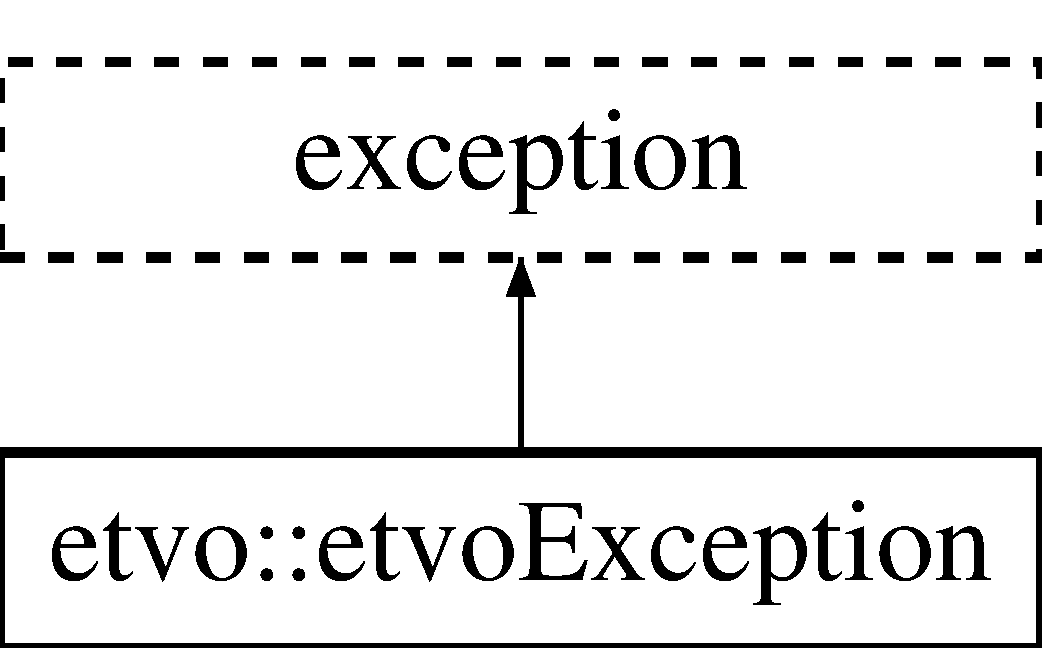
\includegraphics[height=2.000000cm]{classetvo_1_1etvo_exception}
\end{center}
\end{figure}
\subsection*{Public Member Functions}
\begin{DoxyCompactItemize}
\item 
\mbox{\label{classetvo_1_1etvo_exception_af7dacddeb97be42652d39041e8ae8bce}} 
{\bfseries etvo\+Exception} (unsigned num, const std\+::string \&msg)
\item 
\mbox{\label{classetvo_1_1etvo_exception_ae0497a9cc6a09ad55c0a6adc879b2af7}} 
unsigned {\bfseries Num} () const
\item 
\mbox{\label{classetvo_1_1etvo_exception_a124cbbeab0fb4c3701f1a564662b13c5}} 
std\+::string {\bfseries Message} () const
\item 
\mbox{\label{classetvo_1_1etvo_exception_a5727cd8a0d7165e46d5e3877b297773f}} 
virtual const char $\ast$ {\bfseries what} () const  throw ()
\end{DoxyCompactItemize}


\subsection{Detailed Description}
Class to describe exceptions in etvo. 

\begin{DoxyAuthor}{Author}
BC LH JT L\+A\+R\+IS 
\end{DoxyAuthor}
\begin{DoxyVersion}{Version}
2.\+0 
\end{DoxyVersion}


The documentation for this class was generated from the following files\+:\begin{DoxyCompactItemize}
\item 
F\+:/\+U\+A Box/\+Dev\+Soft/etvo\+I\+I\+I/etvo21/etvo/common/\textbf{ etvo\+Exception.\+h}\item 
F\+:/\+U\+A Box/\+Dev\+Soft/etvo\+I\+I\+I/etvo21/etvo/common/etvo\+Exception.\+cpp\end{DoxyCompactItemize}

\section{etvo\+:\+:Fmaxp Class Reference}
\label{classetvo_1_1_fmaxp}\index{etvo\+::\+Fmaxp@{etvo\+::\+Fmaxp}}


Class for pseudo -\/ periodic functions with oplus=max and otimes=composition.  




{\ttfamily \#include $<$Fmaxp.\+h$>$}

Inheritance diagram for etvo\+:\+:Fmaxp\+:\begin{figure}[H]
\begin{center}
\leavevmode
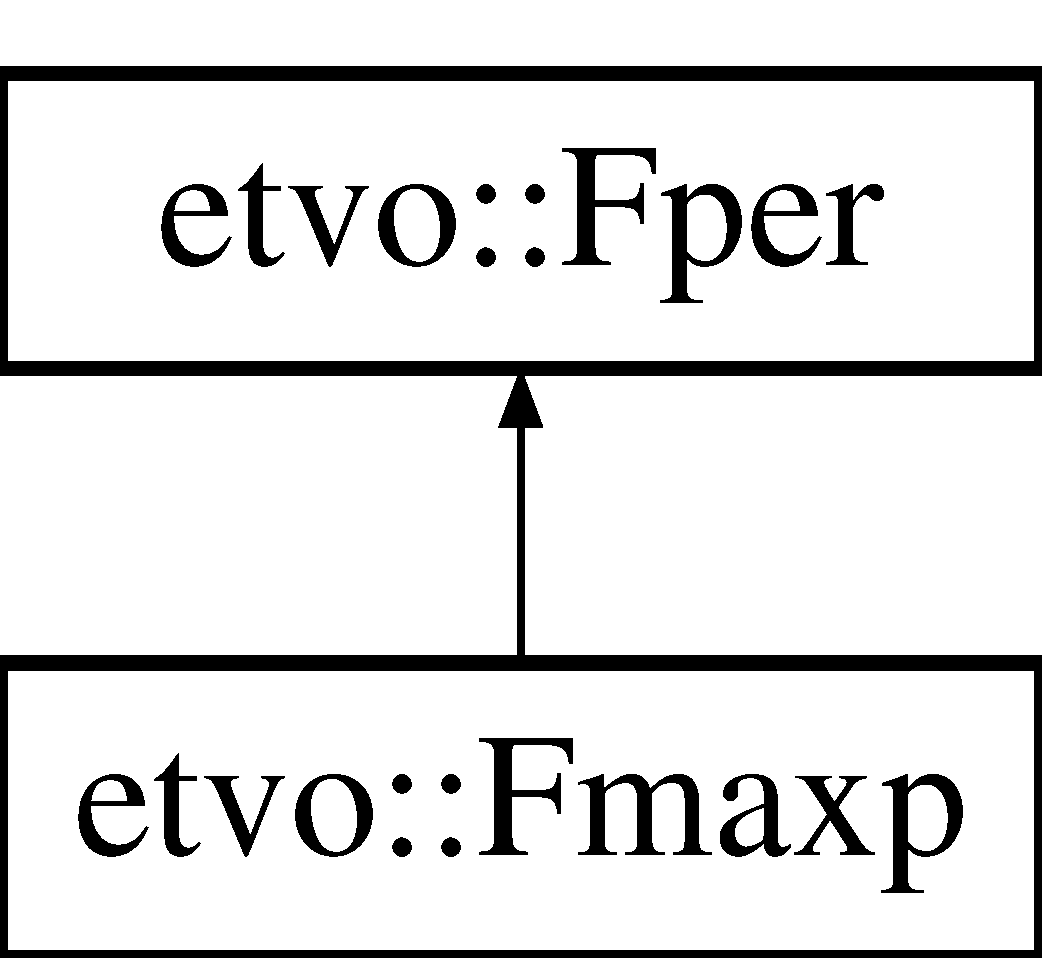
\includegraphics[height=2.000000cm]{classetvo_1_1_fmaxp}
\end{center}
\end{figure}
\subsection*{Public Member Functions}
\begin{DoxyCompactItemize}
\item 
\textbf{ Fmaxp} ()
\item 
\textbf{ Fmaxp} (int dP, int codP, const std\+::vector$<$ int $>$ \&seq)
\item 
\textbf{ Fmaxp} (const \textbf{ Fper} \&)
\item 
\textbf{ Fmaxp} \textbf{ min} (const \textbf{ Fmaxp} \&) const
\item 
\textbf{ Fmaxp} \textbf{ max} (const \textbf{ Fmaxp} \&) const
\item 
\textbf{ Fmaxp} \textbf{ operator+} (const \textbf{ Fmaxp} \&f) const
\item 
\textbf{ Fmaxp} \textbf{ operator$\ast$} (const \textbf{ Fmaxp} \&f) const
\item 
\textbf{ Fmaxp} \textbf{ inf} (const \textbf{ Fmaxp} \&f) const
\item 
\mbox{\label{classetvo_1_1_fmaxp_ad6d47362e103ffb4f34067e88323fb21}} 
bool {\bfseries operator==} (const \textbf{ Fmaxp} \&) const
\item 
\mbox{\label{classetvo_1_1_fmaxp_a814399943888848dc81c9dca6ce5152e}} 
bool {\bfseries operator!=} (const \textbf{ Fmaxp} \&) const
\item 
\mbox{\label{classetvo_1_1_fmaxp_a714673eaa746ba732c0466efff5593f1}} 
bool {\bfseries operator$<$=} (const \textbf{ Fmaxp} \&) const
\item 
\mbox{\label{classetvo_1_1_fmaxp_ac37fe12a520ada748b18eab7af2fa269}} 
bool {\bfseries operator$>$=} (const \textbf{ Fmaxp} \&) const
\item 
\mbox{\label{classetvo_1_1_fmaxp_aeadf3fceebff5caff885b625a6c95b58}} 
bool {\bfseries operator$<$} (const \textbf{ Fmaxp} \&) const
\item 
\mbox{\label{classetvo_1_1_fmaxp_a6d4516a867f8a455205722db5964f093}} 
bool {\bfseries operator$>$} (const \textbf{ Fmaxp} \&) const
\item 
\textbf{ Fmaxp} \textbf{ lfrac} (const \textbf{ Fmaxp} \&a) const
\begin{DoxyCompactList}\small\item\em residuation of the left product \doxyref{Fmaxp}{p.}{classetvo_1_1_fmaxp} g,f; \end{DoxyCompactList}\item 
\textbf{ Fmaxp} \textbf{ rfrac} (const \textbf{ Fmaxp} \&a) const
\begin{DoxyCompactList}\small\item\em residuation of the right product \doxyref{Fmaxp}{p.}{classetvo_1_1_fmaxp} g,f; ... g.\+rfrac(f) = greatest function h s.\+t. h.\+f $<$= g \end{DoxyCompactList}\item 
virtual std\+::string \textbf{ to\+String} () const
\end{DoxyCompactItemize}
\subsection*{Static Public Member Functions}
\begin{DoxyCompactItemize}
\item 
static \textbf{ Fmaxp} \textbf{ E} ()
\end{DoxyCompactItemize}
\subsection*{Additional Inherited Members}


\subsection{Detailed Description}
Class for pseudo -\/ periodic functions with oplus=max and otimes=composition. 

\begin{DoxyAuthor}{Author}
BC LH JT L\+A\+R\+IS 
\end{DoxyAuthor}
\begin{DoxyVersion}{Version}
2.\+0 
\end{DoxyVersion}


\subsection{Constructor \& Destructor Documentation}
\mbox{\label{classetvo_1_1_fmaxp_ae0d1d174539051f9c98a6063a2e502d3}} 
\index{etvo\+::\+Fmaxp@{etvo\+::\+Fmaxp}!Fmaxp@{Fmaxp}}
\index{Fmaxp@{Fmaxp}!etvo\+::\+Fmaxp@{etvo\+::\+Fmaxp}}
\subsubsection{Fmaxp()\hspace{0.1cm}{\footnotesize\ttfamily [1/3]}}
{\footnotesize\ttfamily etvo\+::\+Fmaxp\+::\+Fmaxp (\begin{DoxyParamCaption}{ }\end{DoxyParamCaption})}

Default constructor \+: Id function \mbox{\label{classetvo_1_1_fmaxp_ab2c585af810853b2e4267f2afb0bb20f}} 
\index{etvo\+::\+Fmaxp@{etvo\+::\+Fmaxp}!Fmaxp@{Fmaxp}}
\index{Fmaxp@{Fmaxp}!etvo\+::\+Fmaxp@{etvo\+::\+Fmaxp}}
\subsubsection{Fmaxp()\hspace{0.1cm}{\footnotesize\ttfamily [2/3]}}
{\footnotesize\ttfamily etvo\+::\+Fmaxp\+::\+Fmaxp (\begin{DoxyParamCaption}\item[{int}]{dP,  }\item[{int}]{codP,  }\item[{const std\+::vector$<$ int $>$ \&}]{seq }\end{DoxyParamCaption})}

Constructor\+: full definition (see the base class \doxyref{Fper}{p.}{classetvo_1_1_fper}) \mbox{\label{classetvo_1_1_fmaxp_a2c8a1b9a5953eb0ff7568148434c510d}} 
\index{etvo\+::\+Fmaxp@{etvo\+::\+Fmaxp}!Fmaxp@{Fmaxp}}
\index{Fmaxp@{Fmaxp}!etvo\+::\+Fmaxp@{etvo\+::\+Fmaxp}}
\subsubsection{Fmaxp()\hspace{0.1cm}{\footnotesize\ttfamily [3/3]}}
{\footnotesize\ttfamily etvo\+::\+Fmaxp\+::\+Fmaxp (\begin{DoxyParamCaption}\item[{const \textbf{ Fper} \&}]{f }\end{DoxyParamCaption})}

Constructor\+: initialise from \doxyref{Fper}{p.}{classetvo_1_1_fper} function 

\subsection{Member Function Documentation}
\mbox{\label{classetvo_1_1_fmaxp_a4095f230729e0e62bfb9b556ef815115}} 
\index{etvo\+::\+Fmaxp@{etvo\+::\+Fmaxp}!E@{E}}
\index{E@{E}!etvo\+::\+Fmaxp@{etvo\+::\+Fmaxp}}
\subsubsection{E()}
{\footnotesize\ttfamily \textbf{ Fmaxp} etvo\+::\+Fmaxp\+::E (\begin{DoxyParamCaption}{ }\end{DoxyParamCaption})\hspace{0.3cm}{\ttfamily [static]}}

Class method (called by \doxyref{Fminp\+::\+E()}{p.}{classetvo_1_1_fminp_a4088ca38d381a7e963685fdc788879ac}) returning the Id function \mbox{\label{classetvo_1_1_fmaxp_a0c94b9b2fabef5576f9633b196030f4b}} 
\index{etvo\+::\+Fmaxp@{etvo\+::\+Fmaxp}!inf@{inf}}
\index{inf@{inf}!etvo\+::\+Fmaxp@{etvo\+::\+Fmaxp}}
\subsubsection{inf()}
{\footnotesize\ttfamily \textbf{ Fmaxp} etvo\+::\+Fmaxp\+::inf (\begin{DoxyParamCaption}\item[{const \textbf{ Fmaxp} \&}]{f }\end{DoxyParamCaption}) const}

infimum (min) operation between two functions with the same slope \mbox{\label{classetvo_1_1_fmaxp_a6496a219f52c2f321e2ac02f24638e64}} 
\index{etvo\+::\+Fmaxp@{etvo\+::\+Fmaxp}!lfrac@{lfrac}}
\index{lfrac@{lfrac}!etvo\+::\+Fmaxp@{etvo\+::\+Fmaxp}}
\subsubsection{lfrac()}
{\footnotesize\ttfamily \textbf{ Fmaxp} etvo\+::\+Fmaxp\+::lfrac (\begin{DoxyParamCaption}\item[{const \textbf{ Fmaxp} \&}]{a }\end{DoxyParamCaption}) const}



residuation of the left product \doxyref{Fmaxp}{p.}{classetvo_1_1_fmaxp} g,f; 

...

g.\+lfrac(f) = \char`\"{}greatest\char`\"{} (according to the (max,+) order) function h s.\+t. f.\+h $<$= g a\textbackslash{}b = Max \{x $\vert$ a(x)$<$= b\} forall t, x(t)=max\{ tmax $\vert$ f(tmax)$<$=g(t)\} returns a\textbackslash{}b with b=$\ast$this \mbox{\label{classetvo_1_1_fmaxp_aa203db4eaa908c9320f2a2fea424048f}} 
\index{etvo\+::\+Fmaxp@{etvo\+::\+Fmaxp}!max@{max}}
\index{max@{max}!etvo\+::\+Fmaxp@{etvo\+::\+Fmaxp}}
\subsubsection{max()}
{\footnotesize\ttfamily \textbf{ Fmaxp} etvo\+::\+Fmaxp\+::max (\begin{DoxyParamCaption}\item[{const \textbf{ Fmaxp} \&}]{f }\end{DoxyParamCaption}) const}

max operation between two functions with the same slope cod\+P/dP \mbox{\label{classetvo_1_1_fmaxp_ab7939bb9102e2f5dbfada1385e62e76b}} 
\index{etvo\+::\+Fmaxp@{etvo\+::\+Fmaxp}!min@{min}}
\index{min@{min}!etvo\+::\+Fmaxp@{etvo\+::\+Fmaxp}}
\subsubsection{min()}
{\footnotesize\ttfamily \textbf{ Fmaxp} etvo\+::\+Fmaxp\+::min (\begin{DoxyParamCaption}\item[{const \textbf{ Fmaxp} \&}]{f }\end{DoxyParamCaption}) const}

min operation between two functions with the same slope cod\+P/dP \mbox{\label{classetvo_1_1_fmaxp_ae65bc00a3d0c1a893b43cd76526db4b2}} 
\index{etvo\+::\+Fmaxp@{etvo\+::\+Fmaxp}!operator$\ast$@{operator$\ast$}}
\index{operator$\ast$@{operator$\ast$}!etvo\+::\+Fmaxp@{etvo\+::\+Fmaxp}}
\subsubsection{operator$\ast$()}
{\footnotesize\ttfamily \textbf{ Fmaxp} etvo\+::\+Fmaxp\+::operator$\ast$ (\begin{DoxyParamCaption}\item[{const \textbf{ Fmaxp} \&}]{f }\end{DoxyParamCaption}) const}


\begin{DoxyItemize}
\item operator=composition 
\end{DoxyItemize}\mbox{\label{classetvo_1_1_fmaxp_a29e1c0fe50c158da88fd71816ae150c5}} 
\index{etvo\+::\+Fmaxp@{etvo\+::\+Fmaxp}!operator+@{operator+}}
\index{operator+@{operator+}!etvo\+::\+Fmaxp@{etvo\+::\+Fmaxp}}
\subsubsection{operator+()}
{\footnotesize\ttfamily \textbf{ Fmaxp} etvo\+::\+Fmaxp\+::operator+ (\begin{DoxyParamCaption}\item[{const \textbf{ Fmaxp} \&}]{f }\end{DoxyParamCaption}) const}


\begin{DoxyItemize}
\item operator=max 
\end{DoxyItemize}\mbox{\label{classetvo_1_1_fmaxp_ad7859f4900681c6fb09f9155331e1c1e}} 
\index{etvo\+::\+Fmaxp@{etvo\+::\+Fmaxp}!rfrac@{rfrac}}
\index{rfrac@{rfrac}!etvo\+::\+Fmaxp@{etvo\+::\+Fmaxp}}
\subsubsection{rfrac()}
{\footnotesize\ttfamily \textbf{ Fmaxp} etvo\+::\+Fmaxp\+::rfrac (\begin{DoxyParamCaption}\item[{const \textbf{ Fmaxp} \&}]{a }\end{DoxyParamCaption}) const}



residuation of the right product \doxyref{Fmaxp}{p.}{classetvo_1_1_fmaxp} g,f; ... g.\+rfrac(f) = greatest function h s.\+t. h.\+f $<$= g 

returns b/a (b=$\ast$this)

Fill the begining if not complete \mbox{\label{classetvo_1_1_fmaxp_af21e95c15a7507f3b10ff21b77671139}} 
\index{etvo\+::\+Fmaxp@{etvo\+::\+Fmaxp}!to\+String@{to\+String}}
\index{to\+String@{to\+String}!etvo\+::\+Fmaxp@{etvo\+::\+Fmaxp}}
\subsubsection{to\+String()}
{\footnotesize\ttfamily std\+::string etvo\+::\+Fmaxp\+::to\+String (\begin{DoxyParamCaption}{ }\end{DoxyParamCaption}) const\hspace{0.3cm}{\ttfamily [virtual]}}

returns a string description of the function 

Reimplemented from \textbf{ etvo\+::\+Fper} \doxyref{}{p.}{classetvo_1_1_fper_ad1f4a28d8c2519420ba9cecf1b248302}.



The documentation for this class was generated from the following files\+:\begin{DoxyCompactItemize}
\item 
F\+:/\+U\+A Box/\+Dev\+Soft/etvo\+I\+I\+I/etvo21/etvo/\+Fper/\textbf{ Fmaxp.\+h}\item 
F\+:/\+U\+A Box/\+Dev\+Soft/etvo\+I\+I\+I/etvo21/etvo/\+Fper/Fmaxp.\+cpp\end{DoxyCompactItemize}

\section{etvo\+:\+:Fminp Class Reference}
\label{classetvo_1_1_fminp}\index{etvo\+::\+Fminp@{etvo\+::\+Fminp}}


Class for pseudo -\/ periodic functions with oplus=min and otimes=composition.  




{\ttfamily \#include $<$Fminp.\+h$>$}

Inheritance diagram for etvo\+:\+:Fminp\+:\begin{figure}[H]
\begin{center}
\leavevmode
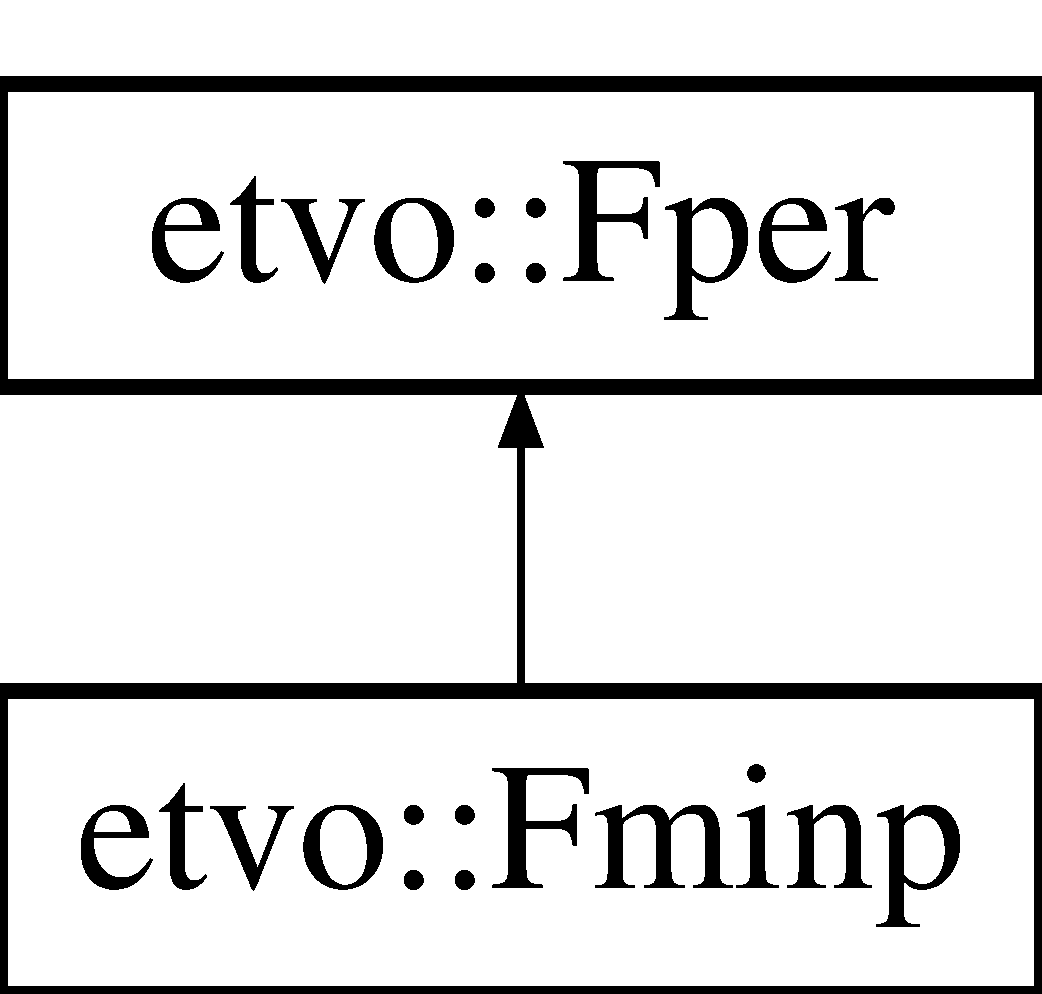
\includegraphics[height=2.000000cm]{classetvo_1_1_fminp}
\end{center}
\end{figure}
\subsection*{Public Member Functions}
\begin{DoxyCompactItemize}
\item 
\textbf{ Fminp} ()
\item 
\textbf{ Fminp} (int dP, int codP, const std\+::vector$<$ int $>$ \&seq)
\item 
\textbf{ Fminp} (const \textbf{ Fper} \&f)
\item 
\textbf{ Fminp} \textbf{ min} (const \textbf{ Fminp} \&f) const
\item 
\textbf{ Fminp} \textbf{ max} (const \textbf{ Fminp} \&f) const
\item 
\textbf{ Fminp} \textbf{ operator+} (const \textbf{ Fminp} \&f) const
\item 
\textbf{ Fminp} \textbf{ operator$\ast$} (const \textbf{ Fminp} \&f) const
\item 
\textbf{ Fminp} \textbf{ inf} (const \textbf{ Fminp} \&f) const
\item 
\textbf{ Fminp} \textbf{ lfrac} (const \textbf{ Fminp} \&a) const
\begin{DoxyCompactList}\small\item\em residuation of the left product \doxyref{Fminp}{p.}{classetvo_1_1_fminp} g,f; \end{DoxyCompactList}\item 
\textbf{ Fminp} \textbf{ rfrac} (const \textbf{ Fminp} \&a) const
\begin{DoxyCompactList}\small\item\em residuation of the right product \doxyref{Fminp}{p.}{classetvo_1_1_fminp} g,f; \end{DoxyCompactList}\item 
\mbox{\label{classetvo_1_1_fminp_a46eb5397b853e77eae0bcf3eff9c4a65}} 
bool {\bfseries operator==} (const \textbf{ Fminp} \&f) const
\item 
\mbox{\label{classetvo_1_1_fminp_a04bf4939906fee060df856c9585d087a}} 
bool {\bfseries operator!=} (const \textbf{ Fminp} \&f) const
\item 
\mbox{\label{classetvo_1_1_fminp_a6355357b68fa3d0531c5fe37bb4a6223}} 
bool {\bfseries operator$<$=} (const \textbf{ Fminp} \&f) const
\item 
\mbox{\label{classetvo_1_1_fminp_ac4de4ee7c0780a87cf047973529ca7bf}} 
bool {\bfseries operator$>$=} (const \textbf{ Fminp} \&f) const
\item 
\mbox{\label{classetvo_1_1_fminp_a935129b770a63d0c1c6622360155a13d}} 
bool {\bfseries operator$<$} (const \textbf{ Fminp} \&f) const
\item 
\mbox{\label{classetvo_1_1_fminp_a7320074ad50b12c621605e1cee53aff2}} 
bool {\bfseries operator$>$} (const \textbf{ Fminp} \&f) const
\item 
virtual std\+::string \textbf{ to\+String} () const
\end{DoxyCompactItemize}
\subsection*{Static Public Member Functions}
\begin{DoxyCompactItemize}
\item 
static \textbf{ Fminp} \textbf{ E} ()
\end{DoxyCompactItemize}
\subsection*{Additional Inherited Members}


\subsection{Detailed Description}
Class for pseudo -\/ periodic functions with oplus=min and otimes=composition. 

\begin{DoxyAuthor}{Author}
BC LH JT L\+A\+R\+IS 
\end{DoxyAuthor}
\begin{DoxyVersion}{Version}
2.\+0 
\end{DoxyVersion}


\subsection{Constructor \& Destructor Documentation}
\mbox{\label{classetvo_1_1_fminp_a3d36c4a488de3e6c89167fcfcc9c1fc9}} 
\index{etvo\+::\+Fminp@{etvo\+::\+Fminp}!Fminp@{Fminp}}
\index{Fminp@{Fminp}!etvo\+::\+Fminp@{etvo\+::\+Fminp}}
\subsubsection{Fminp()\hspace{0.1cm}{\footnotesize\ttfamily [1/3]}}
{\footnotesize\ttfamily etvo\+::\+Fminp\+::\+Fminp (\begin{DoxyParamCaption}{ }\end{DoxyParamCaption})}

Default constructor \+: Id function \mbox{\label{classetvo_1_1_fminp_a0e279734063bf7c894e826d775d732e3}} 
\index{etvo\+::\+Fminp@{etvo\+::\+Fminp}!Fminp@{Fminp}}
\index{Fminp@{Fminp}!etvo\+::\+Fminp@{etvo\+::\+Fminp}}
\subsubsection{Fminp()\hspace{0.1cm}{\footnotesize\ttfamily [2/3]}}
{\footnotesize\ttfamily etvo\+::\+Fminp\+::\+Fminp (\begin{DoxyParamCaption}\item[{int}]{dP,  }\item[{int}]{codP,  }\item[{const std\+::vector$<$ int $>$ \&}]{seq }\end{DoxyParamCaption})}

Constructor\+: full definition (see the base class \doxyref{Fper}{p.}{classetvo_1_1_fper}) \mbox{\label{classetvo_1_1_fminp_a07213f5a1cd1393fd37415aba5dfbbf4}} 
\index{etvo\+::\+Fminp@{etvo\+::\+Fminp}!Fminp@{Fminp}}
\index{Fminp@{Fminp}!etvo\+::\+Fminp@{etvo\+::\+Fminp}}
\subsubsection{Fminp()\hspace{0.1cm}{\footnotesize\ttfamily [3/3]}}
{\footnotesize\ttfamily etvo\+::\+Fminp\+::\+Fminp (\begin{DoxyParamCaption}\item[{const \textbf{ Fper} \&}]{f }\end{DoxyParamCaption})}

Constructor\+: initialise from \doxyref{Fper}{p.}{classetvo_1_1_fper} function 

\subsection{Member Function Documentation}
\mbox{\label{classetvo_1_1_fminp_a4088ca38d381a7e963685fdc788879ac}} 
\index{etvo\+::\+Fminp@{etvo\+::\+Fminp}!E@{E}}
\index{E@{E}!etvo\+::\+Fminp@{etvo\+::\+Fminp}}
\subsubsection{E()}
{\footnotesize\ttfamily \textbf{ Fminp} etvo\+::\+Fminp\+::E (\begin{DoxyParamCaption}{ }\end{DoxyParamCaption})\hspace{0.3cm}{\ttfamily [static]}}

Class method (called by \doxyref{Fminp\+::\+E()}{p.}{classetvo_1_1_fminp_a4088ca38d381a7e963685fdc788879ac}) returning the Id function \mbox{\label{classetvo_1_1_fminp_a9ccc28e1d3ea695d982bf2f83862b335}} 
\index{etvo\+::\+Fminp@{etvo\+::\+Fminp}!inf@{inf}}
\index{inf@{inf}!etvo\+::\+Fminp@{etvo\+::\+Fminp}}
\subsubsection{inf()}
{\footnotesize\ttfamily \textbf{ Fminp} etvo\+::\+Fminp\+::inf (\begin{DoxyParamCaption}\item[{const \textbf{ Fminp} \&}]{f }\end{DoxyParamCaption}) const}

infimum (max) operation between two functions with the same slope \mbox{\label{classetvo_1_1_fminp_a8792d12ff6a5319c46b3be736a41d8e9}} 
\index{etvo\+::\+Fminp@{etvo\+::\+Fminp}!lfrac@{lfrac}}
\index{lfrac@{lfrac}!etvo\+::\+Fminp@{etvo\+::\+Fminp}}
\subsubsection{lfrac()}
{\footnotesize\ttfamily \textbf{ Fminp} etvo\+::\+Fminp\+::lfrac (\begin{DoxyParamCaption}\item[{const \textbf{ Fminp} \&}]{a }\end{DoxyParamCaption}) const}



residuation of the left product \doxyref{Fminp}{p.}{classetvo_1_1_fminp} g,f; 

...

g.\+lfrac(f) = \char`\"{}greatest\char`\"{} (according to the (min,+) order) function h s.\+t. f.\+h $<$= g a\textbackslash{}b = Min \{x $\vert$ a(x)$>$= b\} forall k, x(k)=min\{ kmin $\vert$ f(kmin)$>$=g(k)\} ~\newline
~\newline
 returns a\textbackslash{}b with b=$\ast$this

result periodicity \mbox{\label{classetvo_1_1_fminp_a5dc06185c4307fc3001ed17730a18b6f}} 
\index{etvo\+::\+Fminp@{etvo\+::\+Fminp}!max@{max}}
\index{max@{max}!etvo\+::\+Fminp@{etvo\+::\+Fminp}}
\subsubsection{max()}
{\footnotesize\ttfamily \textbf{ Fminp} etvo\+::\+Fminp\+::max (\begin{DoxyParamCaption}\item[{const \textbf{ Fminp} \&}]{f }\end{DoxyParamCaption}) const}

max operation between two functions with the same slope cod\+P/dP \mbox{\label{classetvo_1_1_fminp_a07d73d800d86a665acff1b79f6898ba8}} 
\index{etvo\+::\+Fminp@{etvo\+::\+Fminp}!min@{min}}
\index{min@{min}!etvo\+::\+Fminp@{etvo\+::\+Fminp}}
\subsubsection{min()}
{\footnotesize\ttfamily \textbf{ Fminp} etvo\+::\+Fminp\+::min (\begin{DoxyParamCaption}\item[{const \textbf{ Fminp} \&}]{f }\end{DoxyParamCaption}) const}

min operation between two functions with the same slope cod\+P/dP \mbox{\label{classetvo_1_1_fminp_a57fb37d7fba34df7a1ea560b121b8a56}} 
\index{etvo\+::\+Fminp@{etvo\+::\+Fminp}!operator$\ast$@{operator$\ast$}}
\index{operator$\ast$@{operator$\ast$}!etvo\+::\+Fminp@{etvo\+::\+Fminp}}
\subsubsection{operator$\ast$()}
{\footnotesize\ttfamily \textbf{ Fminp} etvo\+::\+Fminp\+::operator$\ast$ (\begin{DoxyParamCaption}\item[{const \textbf{ Fminp} \&}]{f }\end{DoxyParamCaption}) const}


\begin{DoxyItemize}
\item operator = composition 
\end{DoxyItemize}\mbox{\label{classetvo_1_1_fminp_a32835366b9c1e4829e8b8583e1ec31c2}} 
\index{etvo\+::\+Fminp@{etvo\+::\+Fminp}!operator+@{operator+}}
\index{operator+@{operator+}!etvo\+::\+Fminp@{etvo\+::\+Fminp}}
\subsubsection{operator+()}
{\footnotesize\ttfamily \textbf{ Fminp} etvo\+::\+Fminp\+::operator+ (\begin{DoxyParamCaption}\item[{const \textbf{ Fminp} \&}]{f }\end{DoxyParamCaption}) const}


\begin{DoxyItemize}
\item operator=min 
\end{DoxyItemize}\mbox{\label{classetvo_1_1_fminp_a4faa552bcbf49ba6eebef024d69338c6}} 
\index{etvo\+::\+Fminp@{etvo\+::\+Fminp}!rfrac@{rfrac}}
\index{rfrac@{rfrac}!etvo\+::\+Fminp@{etvo\+::\+Fminp}}
\subsubsection{rfrac()}
{\footnotesize\ttfamily \textbf{ Fminp} etvo\+::\+Fminp\+::rfrac (\begin{DoxyParamCaption}\item[{const \textbf{ Fminp} \&}]{a }\end{DoxyParamCaption}) const}



residuation of the right product \doxyref{Fminp}{p.}{classetvo_1_1_fminp} g,f; 

...

g.\+rfrac(f) = greatest function h s.\+t. h.\+f $<$= g returns b/a (b=$\ast$this) \mbox{\label{classetvo_1_1_fminp_a498d19bc5563949ce9028a4c44e69463}} 
\index{etvo\+::\+Fminp@{etvo\+::\+Fminp}!to\+String@{to\+String}}
\index{to\+String@{to\+String}!etvo\+::\+Fminp@{etvo\+::\+Fminp}}
\subsubsection{to\+String()}
{\footnotesize\ttfamily std\+::string etvo\+::\+Fminp\+::to\+String (\begin{DoxyParamCaption}{ }\end{DoxyParamCaption}) const\hspace{0.3cm}{\ttfamily [virtual]}}

returns a string description of the function 

Reimplemented from \textbf{ etvo\+::\+Fper} \doxyref{}{p.}{classetvo_1_1_fper_ad1f4a28d8c2519420ba9cecf1b248302}.



The documentation for this class was generated from the following files\+:\begin{DoxyCompactItemize}
\item 
F\+:/\+U\+A Box/\+Dev\+Soft/etvo\+I\+I\+I/etvo21/etvo/\+Fper/\textbf{ Fminp.\+h}\item 
F\+:/\+U\+A Box/\+Dev\+Soft/etvo\+I\+I\+I/etvo21/etvo/\+Fper/Fminp.\+cpp\end{DoxyCompactItemize}

\section{etvo\+:\+:Fper Class Reference}
\label{classetvo_1_1_fper}\index{etvo\+::\+Fper@{etvo\+::\+Fper}}


Base class for pseudo -\/ periodic functions Z-\/$>$Z where f(x + dP) = codP + f(x)  




{\ttfamily \#include $<$Fper.\+h$>$}

Inheritance diagram for etvo\+:\+:Fper\+:\begin{figure}[H]
\begin{center}
\leavevmode
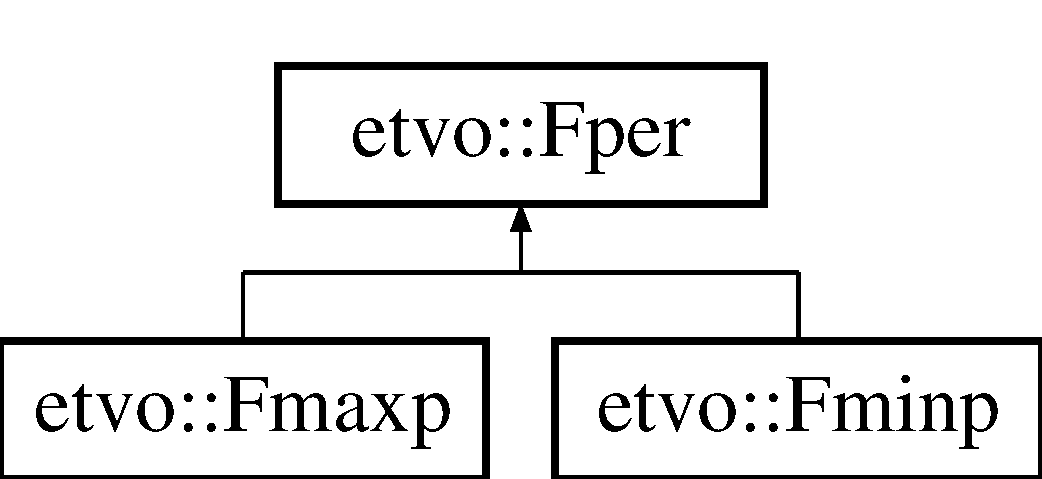
\includegraphics[height=2.000000cm]{classetvo_1_1_fper}
\end{center}
\end{figure}
\subsection*{Public Member Functions}
\begin{DoxyCompactItemize}
\item 
\mbox{\label{classetvo_1_1_fper_a6594dc69c1e42ab3cc761c90c74153a9}} 
\textbf{ Fper} ()
\begin{DoxyCompactList}\small\item\em Default constructor \+: set as Id function Z-\/$>$Z,x-\/$>$x. \end{DoxyCompactList}\item 
\textbf{ Fper} (int dP, int codP, const std\+::vector$<$ int $>$ \&seq)
\begin{DoxyCompactList}\small\item\em Constructor \+: full definition. \end{DoxyCompactList}\item 
void \textbf{ set\+Seq} (const std\+::vector$<$ int $>$ \&seq)
\begin{DoxyCompactList}\small\item\em Set values of f(0),f(1), ... over one period. \end{DoxyCompactList}\item 
void \textbf{ set\+Periodicity} (int dP, int codP)
\begin{DoxyCompactList}\small\item\em Set d\+P/codP. \end{DoxyCompactList}\item 
int \textbf{ get\+Value} (int arg) const
\begin{DoxyCompactList}\small\item\em Value of f(x) \end{DoxyCompactList}\item 
int \textbf{ operator()} (int arg) const
\begin{DoxyCompactList}\small\item\em Value of f(x) \end{DoxyCompactList}\item 
\mbox{\label{classetvo_1_1_fper_a7c95500da53639792f127fbaa6599000}} 
bool {\bfseries operator==} (const \textbf{ Fper} \&f) const
\item 
\mbox{\label{classetvo_1_1_fper_ae2bd6d08aa9c2d6ff30de7e300e4d829}} 
bool {\bfseries operator!=} (const \textbf{ Fper} \&f) const
\item 
\mbox{\label{classetvo_1_1_fper_a9c9b02ee4d0a82e15b4f34b43e9da43f}} 
bool {\bfseries operator$<$=} (const \textbf{ Fper} \&f) const
\item 
\mbox{\label{classetvo_1_1_fper_af484562d34b883cc8d39995ae2188f6c}} 
bool {\bfseries operator$>$=} (const \textbf{ Fper} \&f) const
\item 
\mbox{\label{classetvo_1_1_fper_a97b70ed2fab8b6237592a4dd5e4936be}} 
std\+::pair$<$ int, int $>$ \textbf{ get\+Periodicity} () const
\begin{DoxyCompactList}\small\item\em returns the pair (dP,codP) \end{DoxyCompactList}\item 
int \textbf{ get\+Dom\+Per} () const
\item 
int \textbf{ get\+Codom\+Per} () const
\item 
\mbox{\label{classetvo_1_1_fper_aab73972f15baf5ad0afecdae00b327e2}} 
\textbf{ Fper} \textbf{ extend\+By} (unsigned mul) const
\begin{DoxyCompactList}\small\item\em Produces a non-\/canonical extension of a (dP,codP) pseudo-\/periodic function The result is the equivalent (mulxdP,mulxcodP) pseudo-\/periodc function. \end{DoxyCompactList}\item 
\textbf{ Fper} \textbf{ compose\+With} (const \textbf{ Fper} \&f) const
\begin{DoxyCompactList}\small\item\em Computes the composition of $\ast$this with f. \end{DoxyCompactList}\item 
\mbox{\label{classetvo_1_1_fper_ae13f594da0ec1ed58b8c3e208008bd8c}} 
void \textbf{ reduce} ()
\begin{DoxyCompactList}\small\item\em Reduces a non-\/canonical pseudo-\/periodic function to the canonical form which has the least period (dP,codP) \end{DoxyCompactList}\item 
\mbox{\label{classetvo_1_1_fper_a60a5a12b6ff782823653cb77d13dc407}} 
void {\bfseries canon} ()
\item 
double \textbf{ gety\+Max0} () const
\item 
double \textbf{ gety\+Min0} () const
\item 
virtual std\+::string \textbf{ to\+String} () const
\end{DoxyCompactItemize}
\subsection*{Static Public Member Functions}
\begin{DoxyCompactItemize}
\item 
\mbox{\label{classetvo_1_1_fper_a4daeece372795ecbf12840318cf10729}} 
static void \textbf{ set\+Auto\+Reduction} (bool on)
\begin{DoxyCompactList}\small\item\em Class method (called by Fper\+::set\+Auto\+Reduction\+State(b)) to set the autoreduction state (O\+N/\+O\+FF) \end{DoxyCompactList}\item 
\mbox{\label{classetvo_1_1_fper_a4979d4b48c92bfca22d5369cb724d5be}} 
static bool \textbf{ get\+Auto\+Reduction\+State} ()
\begin{DoxyCompactList}\small\item\em Class method (called by \doxyref{Fper\+::get\+Auto\+Reduction\+State()}{p.}{classetvo_1_1_fper_a4979d4b48c92bfca22d5369cb724d5be}) to obtain the autoreduction state (O\+N/\+O\+FF) \end{DoxyCompactList}\end{DoxyCompactItemize}
\subsection*{Protected Member Functions}
\begin{DoxyCompactItemize}
\item 
\mbox{\label{classetvo_1_1_fper_af0594d84117f2030eed6a656c5c8d04e}} 
bool {\bfseries reduce\+By} (unsigned div)
\item 
\mbox{\label{classetvo_1_1_fper_a24f7dc3569ac14ae0dd6232aab5f35df}} 
void {\bfseries update\+Y\+Min\+Max} ()
\item 
\mbox{\label{classetvo_1_1_fper_ad0c0ddec58325201d08ba7d8fcfda97b}} 
bool {\bfseries is\+Nodecreasing} (const std\+::vector$<$ int $>$ \&v)
\end{DoxyCompactItemize}
\subsection*{Protected Attributes}
\begin{DoxyCompactItemize}
\item 
\mbox{\label{classetvo_1_1_fper_a224e0499d9eaab7b1304e4ff6970d4c2}} 
int \textbf{ \+\_\+domP}
\begin{DoxyCompactList}\small\item\em domain period \end{DoxyCompactList}\item 
\mbox{\label{classetvo_1_1_fper_a384e158d85b4f1a852c1bb22bd6ad5c7}} 
int \textbf{ \+\_\+codomP}
\begin{DoxyCompactList}\small\item\em codomain period \end{DoxyCompactList}\item 
\mbox{\label{classetvo_1_1_fper_a6a1a9c5a95a910415dae35d997cd12e4}} 
std\+::vector$<$ int $>$ \textbf{ \+\_\+seq}
\begin{DoxyCompactList}\small\item\em periodic sequence \end{DoxyCompactList}\item 
\mbox{\label{classetvo_1_1_fper_aa7795d78964c9333a343052071d1045b}} 
double {\bfseries \+\_\+y\+Max0}
\item 
\mbox{\label{classetvo_1_1_fper_a436d74a7514e66162c004e9efb31f55e}} 
double {\bfseries \+\_\+y\+Min0}
\end{DoxyCompactItemize}
\subsection*{Static Protected Attributes}
\begin{DoxyCompactItemize}
\item 
static bool \textbf{ \+\_\+autoreduction} =true
\begin{DoxyCompactList}\small\item\em class variable to set O\+N/\+O\+FF the autoreduction \end{DoxyCompactList}\end{DoxyCompactItemize}


\subsection{Detailed Description}
Base class for pseudo -\/ periodic functions Z-\/$>$Z where f(x + dP) = codP + f(x) 

\begin{DoxyAuthor}{Author}
BC LH JT L\+A\+R\+IS 
\end{DoxyAuthor}
\begin{DoxyVersion}{Version}
2.\+0 
\end{DoxyVersion}


\subsection{Constructor \& Destructor Documentation}
\mbox{\label{classetvo_1_1_fper_a7db375de96bd6a1279b083d11b079a0e}} 
\index{etvo\+::\+Fper@{etvo\+::\+Fper}!Fper@{Fper}}
\index{Fper@{Fper}!etvo\+::\+Fper@{etvo\+::\+Fper}}
\subsubsection{Fper()}
{\footnotesize\ttfamily etvo\+::\+Fper\+::\+Fper (\begin{DoxyParamCaption}\item[{int}]{dP,  }\item[{int}]{codP,  }\item[{const std\+::vector$<$ int $>$ \&}]{seq }\end{DoxyParamCaption})}



Constructor \+: full definition. 


\begin{DoxyParams}{Parameters}
{\em dP} & domain period \\
\hline
{\em codP} & codomain period \\
\hline
{\em seq} & \+: values of f(0),f(1), ... over one period \\
\hline
\end{DoxyParams}


\subsection{Member Function Documentation}
\mbox{\label{classetvo_1_1_fper_a8f7d8cf4034dfa6ba6b40e09f7faa39e}} 
\index{etvo\+::\+Fper@{etvo\+::\+Fper}!compose\+With@{compose\+With}}
\index{compose\+With@{compose\+With}!etvo\+::\+Fper@{etvo\+::\+Fper}}
\subsubsection{compose\+With()}
{\footnotesize\ttfamily \textbf{ Fper} etvo\+::\+Fper\+::compose\+With (\begin{DoxyParamCaption}\item[{const \textbf{ Fper} \&}]{f }\end{DoxyParamCaption}) const}



Computes the composition of $\ast$this with f. 


\begin{DoxyParams}{Parameters}
{\em f} & an \doxyref{Fper}{p.}{classetvo_1_1_fper} object \\
\hline
\end{DoxyParams}
\begin{DoxyReturn}{Returns}
an \doxyref{Fper}{p.}{classetvo_1_1_fper} object 
\end{DoxyReturn}
\mbox{\label{classetvo_1_1_fper_a245b174b519cccd07dfa8c6d03a0cbeb}} 
\index{etvo\+::\+Fper@{etvo\+::\+Fper}!get\+Codom\+Per@{get\+Codom\+Per}}
\index{get\+Codom\+Per@{get\+Codom\+Per}!etvo\+::\+Fper@{etvo\+::\+Fper}}
\subsubsection{get\+Codom\+Per()}
{\footnotesize\ttfamily int etvo\+::\+Fper\+::get\+Codom\+Per (\begin{DoxyParamCaption}{ }\end{DoxyParamCaption}) const}

returns the codomain period codP \mbox{\label{classetvo_1_1_fper_a1429629d4813a38e83a0699a12fa9c89}} 
\index{etvo\+::\+Fper@{etvo\+::\+Fper}!get\+Dom\+Per@{get\+Dom\+Per}}
\index{get\+Dom\+Per@{get\+Dom\+Per}!etvo\+::\+Fper@{etvo\+::\+Fper}}
\subsubsection{get\+Dom\+Per()}
{\footnotesize\ttfamily int etvo\+::\+Fper\+::get\+Dom\+Per (\begin{DoxyParamCaption}{ }\end{DoxyParamCaption}) const}

returns the domain period dP \mbox{\label{classetvo_1_1_fper_aec63a99ef1520af08e35b12e726fe085}} 
\index{etvo\+::\+Fper@{etvo\+::\+Fper}!get\+Value@{get\+Value}}
\index{get\+Value@{get\+Value}!etvo\+::\+Fper@{etvo\+::\+Fper}}
\subsubsection{get\+Value()}
{\footnotesize\ttfamily int etvo\+::\+Fper\+::get\+Value (\begin{DoxyParamCaption}\item[{int}]{arg }\end{DoxyParamCaption}) const}



Value of f(x) 


\begin{DoxyParams}{Parameters}
{\em arg} & x \\
\hline
\end{DoxyParams}
\begin{DoxyReturn}{Returns}
f(x) 
\end{DoxyReturn}
\mbox{\label{classetvo_1_1_fper_a3a44423e8af95b3fa705aba0bcb7c8b2}} 
\index{etvo\+::\+Fper@{etvo\+::\+Fper}!gety\+Max0@{gety\+Max0}}
\index{gety\+Max0@{gety\+Max0}!etvo\+::\+Fper@{etvo\+::\+Fper}}
\subsubsection{gety\+Max0()}
{\footnotesize\ttfamily double etvo\+::\+Fper\+::gety\+Max0 (\begin{DoxyParamCaption}{ }\end{DoxyParamCaption}) const}

gives the maximum of f(x) projected on y axis [x=0] parallel to (dP,codP) line This value is important for improving max,min computation between functions \mbox{\label{classetvo_1_1_fper_a9ac3a7e1ba800636b5b046996f10d9d8}} 
\index{etvo\+::\+Fper@{etvo\+::\+Fper}!gety\+Min0@{gety\+Min0}}
\index{gety\+Min0@{gety\+Min0}!etvo\+::\+Fper@{etvo\+::\+Fper}}
\subsubsection{gety\+Min0()}
{\footnotesize\ttfamily double etvo\+::\+Fper\+::gety\+Min0 (\begin{DoxyParamCaption}{ }\end{DoxyParamCaption}) const}

gives the minimum of f(x) projected on y axis [x=0] parallel to (dP,codP) line This value is important for improving max,min computation between functions \mbox{\label{classetvo_1_1_fper_affe7ba991ae109ddfdd7935ce3ea6d09}} 
\index{etvo\+::\+Fper@{etvo\+::\+Fper}!operator()@{operator()}}
\index{operator()@{operator()}!etvo\+::\+Fper@{etvo\+::\+Fper}}
\subsubsection{operator()()}
{\footnotesize\ttfamily int etvo\+::\+Fper\+::operator() (\begin{DoxyParamCaption}\item[{int}]{arg }\end{DoxyParamCaption}) const}



Value of f(x) 


\begin{DoxyParams}{Parameters}
{\em arg} & x \\
\hline
\end{DoxyParams}
\begin{DoxyReturn}{Returns}
f(x) 
\end{DoxyReturn}
\mbox{\label{classetvo_1_1_fper_abfe4dd602ac3a34c3bcd8c7ea39d8260}} 
\index{etvo\+::\+Fper@{etvo\+::\+Fper}!set\+Periodicity@{set\+Periodicity}}
\index{set\+Periodicity@{set\+Periodicity}!etvo\+::\+Fper@{etvo\+::\+Fper}}
\subsubsection{set\+Periodicity()}
{\footnotesize\ttfamily void etvo\+::\+Fper\+::set\+Periodicity (\begin{DoxyParamCaption}\item[{int}]{dP,  }\item[{int}]{codP }\end{DoxyParamCaption})}



Set d\+P/codP. 


\begin{DoxyParams}{Parameters}
{\em dP} & domain period \\
\hline
{\em codP} & codomain period \\
\hline
\end{DoxyParams}
\mbox{\label{classetvo_1_1_fper_ac791ffa39ecb3bccd89ec981526bd5a1}} 
\index{etvo\+::\+Fper@{etvo\+::\+Fper}!set\+Seq@{set\+Seq}}
\index{set\+Seq@{set\+Seq}!etvo\+::\+Fper@{etvo\+::\+Fper}}
\subsubsection{set\+Seq()}
{\footnotesize\ttfamily void etvo\+::\+Fper\+::set\+Seq (\begin{DoxyParamCaption}\item[{const std\+::vector$<$ int $>$ \&}]{seq }\end{DoxyParamCaption})}



Set values of f(0),f(1), ... over one period. 


\begin{DoxyParams}{Parameters}
{\em seq} & \+: values of f(0),f(1), \\
\hline
\end{DoxyParams}
\mbox{\label{classetvo_1_1_fper_ad1f4a28d8c2519420ba9cecf1b248302}} 
\index{etvo\+::\+Fper@{etvo\+::\+Fper}!to\+String@{to\+String}}
\index{to\+String@{to\+String}!etvo\+::\+Fper@{etvo\+::\+Fper}}
\subsubsection{to\+String()}
{\footnotesize\ttfamily std\+::string etvo\+::\+Fper\+::to\+String (\begin{DoxyParamCaption}{ }\end{DoxyParamCaption}) const\hspace{0.3cm}{\ttfamily [virtual]}}

Returns a string description of a pseudo-\/periodic function Ex\+: \char`\"{}[-\/7 -\/7 -\/3 -\/3 ](4,5)\char`\"{} for a (4,5) pseudo-\/periodic function f(0)=-\/7,f(1)=-\/7,f(2)=-\/3 ... 

Reimplemented in \textbf{ etvo\+::\+Fminp} \doxyref{}{p.}{classetvo_1_1_fminp_a498d19bc5563949ce9028a4c44e69463}, and \textbf{ etvo\+::\+Fmaxp} \doxyref{}{p.}{classetvo_1_1_fmaxp_af21e95c15a7507f3b10ff21b77671139}.



\subsection{Member Data Documentation}
\mbox{\label{classetvo_1_1_fper_a360fe3522dab4ddbe42f533e932e6ee2}} 
\index{etvo\+::\+Fper@{etvo\+::\+Fper}!\+\_\+autoreduction@{\+\_\+autoreduction}}
\index{\+\_\+autoreduction@{\+\_\+autoreduction}!etvo\+::\+Fper@{etvo\+::\+Fper}}
\subsubsection{\+\_\+autoreduction}
{\footnotesize\ttfamily bool etvo\+::\+Fper\+::\+\_\+autoreduction =true\hspace{0.3cm}{\ttfamily [static]}, {\ttfamily [protected]}}



class variable to set O\+N/\+O\+FF the autoreduction 

autoreduction mode default = ON 

The documentation for this class was generated from the following files\+:\begin{DoxyCompactItemize}
\item 
F\+:/\+U\+A Box/\+Dev\+Soft/etvo\+I\+I\+I/etvo21/etvo/\+Fper/\textbf{ Fper.\+h}\item 
F\+:/\+U\+A Box/\+Dev\+Soft/etvo\+I\+I\+I/etvo21/etvo/\+Fper/\textbf{ Fper.\+cpp}\end{DoxyCompactItemize}

\hypertarget{classmmgd_1_1gd}{}\section{mmgd\+:\+:gd Class Reference}
\label{classmmgd_1_1gd}\index{mmgd\+::gd@{mmgd\+::gd}}
Inheritance diagram for mmgd\+:\+:gd\+:\begin{figure}[H]
\begin{center}
\leavevmode
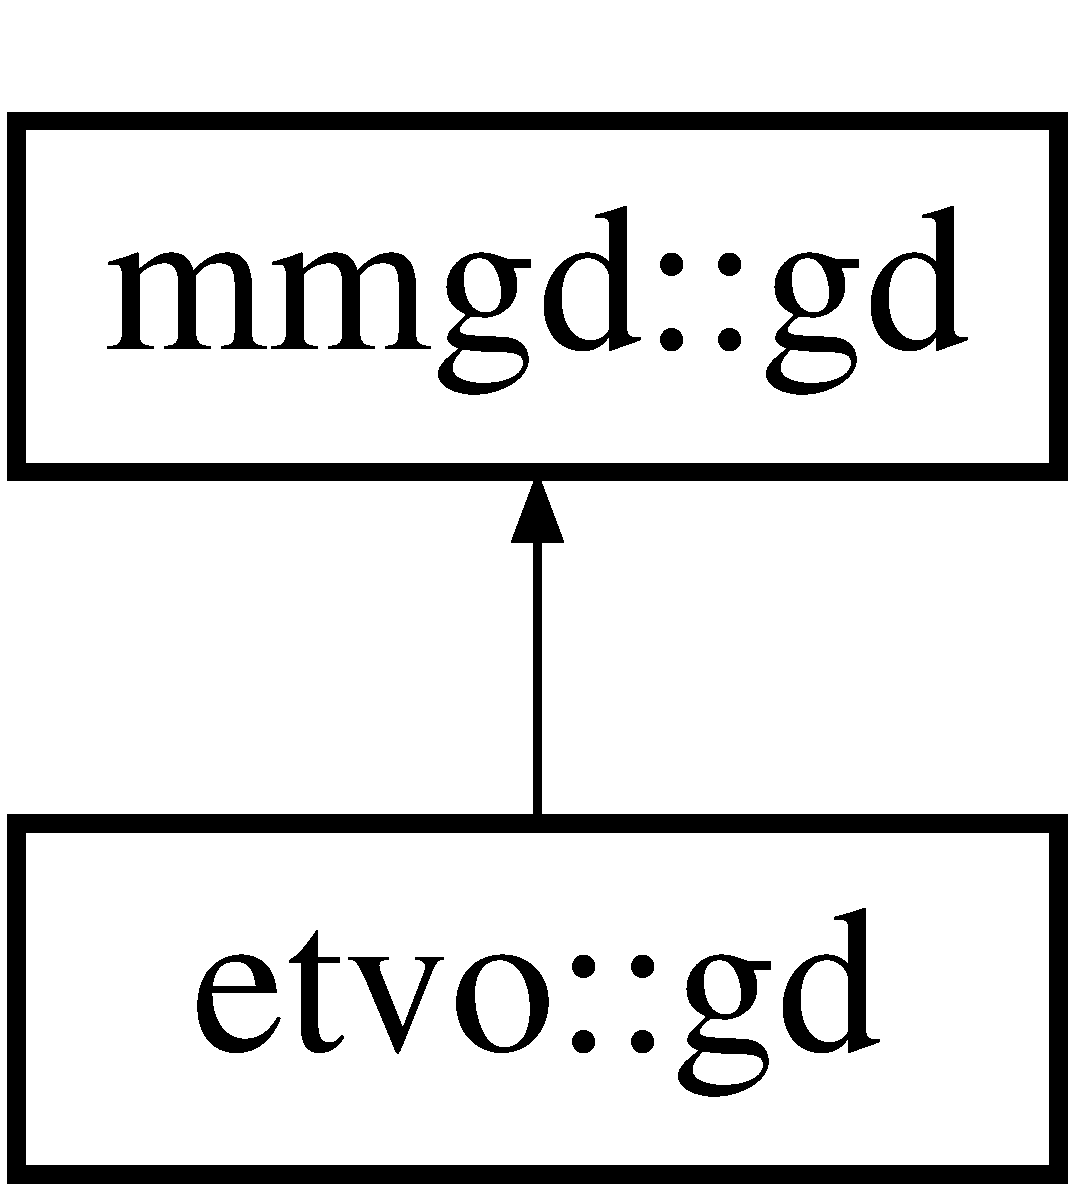
\includegraphics[height=2.000000cm]{classmmgd_1_1gd}
\end{center}
\end{figure}
\subsection*{Public Member Functions}
\begin{DoxyCompactItemize}
\item 
\mbox{\Hypertarget{classmmgd_1_1gd_ac8e74872b52997c0aa6090b82d721e08}\label{classmmgd_1_1gd_ac8e74872b52997c0aa6090b82d721e08}} 
{\bfseries gd} (const \mbox{\hyperlink{classmmgd_1_1gd}{gd}} \&)
\item 
\mbox{\Hypertarget{classmmgd_1_1gd_a512d9003aff50f7b7d2185d7e7272ac6}\label{classmmgd_1_1gd_a512d9003aff50f7b7d2185d7e7272ac6}} 
{\bfseries gd} (long, long)
\item 
\mbox{\Hypertarget{classmmgd_1_1gd_a050613b096bdf3cb95a46d8a207b92cd}\label{classmmgd_1_1gd_a050613b096bdf3cb95a46d8a207b92cd}} 
\mbox{\hyperlink{classmmgd_1_1gd}{gd}} \& {\bfseries operator=} (const \mbox{\hyperlink{classmmgd_1_1gd}{gd}} \&)
\item 
\mbox{\Hypertarget{classmmgd_1_1gd_aceb773d2d343c2c0b9a14f6030d0ac62}\label{classmmgd_1_1gd_aceb773d2d343c2c0b9a14f6030d0ac62}} 
int {\bfseries operator!=} (const \mbox{\hyperlink{classmmgd_1_1gd}{gd}} \&)
\item 
\mbox{\Hypertarget{classmmgd_1_1gd_a4ff3fb6e099001641de565a933d4d898}\label{classmmgd_1_1gd_a4ff3fb6e099001641de565a933d4d898}} 
int {\bfseries operator==} (const \mbox{\hyperlink{classmmgd_1_1gd}{gd}} \&)
\item 
\mbox{\Hypertarget{classmmgd_1_1gd_acfc56cfcff1288f8f4b6120394e7548f}\label{classmmgd_1_1gd_acfc56cfcff1288f8f4b6120394e7548f}} 
int {\bfseries operator$>$=} (const \mbox{\hyperlink{classmmgd_1_1gd}{gd}} \&)
\item 
\mbox{\Hypertarget{classmmgd_1_1gd_a3e38156b0cf3e7cd0a22ba765b874e26}\label{classmmgd_1_1gd_a3e38156b0cf3e7cd0a22ba765b874e26}} 
int {\bfseries operator$<$=} (const \mbox{\hyperlink{classmmgd_1_1gd}{gd}} \&)
\item 
\mbox{\Hypertarget{classmmgd_1_1gd_a89fc335c8bfe23cef630b06e8f1ae507}\label{classmmgd_1_1gd_a89fc335c8bfe23cef630b06e8f1ae507}} 
bool {\bfseries operator$<$} (const \mbox{\hyperlink{classmmgd_1_1gd}{gd}} \&) const
\item 
\mbox{\Hypertarget{classmmgd_1_1gd_a2d04acd086664d7880a2a39ffef3588d}\label{classmmgd_1_1gd_a2d04acd086664d7880a2a39ffef3588d}} 
\mbox{\hyperlink{classmmgd_1_1gd}{gd}} \& {\bfseries init} (long, long)
\item 
\mbox{\Hypertarget{classmmgd_1_1gd_a473a1d68f6362c8b8e7f48aeb38e6461}\label{classmmgd_1_1gd_a473a1d68f6362c8b8e7f48aeb38e6461}} 
\mbox{\hyperlink{classmmgd_1_1gd}{gd}} \& {\bfseries operator()} (long, long)
\item 
\mbox{\Hypertarget{classmmgd_1_1gd_ab452d60ee78b36d09dda2f587f908ce6}\label{classmmgd_1_1gd_ab452d60ee78b36d09dda2f587f908ce6}} 
long {\bfseries getg} (void)
\item 
\mbox{\Hypertarget{classmmgd_1_1gd_af0875481e5b2d5de2f9a2e8a8500aa05}\label{classmmgd_1_1gd_af0875481e5b2d5de2f9a2e8a8500aa05}} 
long {\bfseries getd} (void)
\end{DoxyCompactItemize}
\subsection*{Static Public Attributes}
\begin{DoxyCompactItemize}
\item 
\mbox{\Hypertarget{classmmgd_1_1gd_a406d8038e331c71ec13b5dd00f134207}\label{classmmgd_1_1gd_a406d8038e331c71ec13b5dd00f134207}} 
static \mbox{\hyperlink{classmmgd_1_1gd}{gd}} {\bfseries Top}
\item 
\mbox{\Hypertarget{classmmgd_1_1gd_a066162305c8f563ea3e3bab929c6e94a}\label{classmmgd_1_1gd_a066162305c8f563ea3e3bab929c6e94a}} 
static \mbox{\hyperlink{classmmgd_1_1gd}{gd}} {\bfseries epsilon}
\item 
\mbox{\Hypertarget{classmmgd_1_1gd_afd7496b861bcfa4313382867e16f5ff6}\label{classmmgd_1_1gd_afd7496b861bcfa4313382867e16f5ff6}} 
static \mbox{\hyperlink{classmmgd_1_1gd}{gd}} {\bfseries e}
\end{DoxyCompactItemize}
\subsection*{Protected Member Functions}
\begin{DoxyCompactItemize}
\item 
\mbox{\Hypertarget{classmmgd_1_1gd_a9f0cbddb58f4e9e1c89d03263589af88}\label{classmmgd_1_1gd_a9f0cbddb58f4e9e1c89d03263589af88}} 
void {\bfseries affecte} (long, long)
\end{DoxyCompactItemize}
\subsection*{Protected Attributes}
\begin{DoxyCompactItemize}
\item 
\mbox{\Hypertarget{classmmgd_1_1gd_a4d509ea069575b9c3c4719ebfbfdee59}\label{classmmgd_1_1gd_a4d509ea069575b9c3c4719ebfbfdee59}} 
long {\bfseries g}
\item 
\mbox{\Hypertarget{classmmgd_1_1gd_ab00168800630d031f671ad7057b05aba}\label{classmmgd_1_1gd_ab00168800630d031f671ad7057b05aba}} 
long {\bfseries d}
\end{DoxyCompactItemize}
\subsection*{Friends}
\begin{DoxyCompactItemize}
\item 
\mbox{\Hypertarget{classmmgd_1_1gd_ae6debbf0c1df1dfa98cc657c12c878c1}\label{classmmgd_1_1gd_ae6debbf0c1df1dfa98cc657c12c878c1}} 
std\+::ostream \& {\bfseries operator$<$$<$} (std\+::ostream \&, \mbox{\hyperlink{classmmgd_1_1gd}{gd}} \&)
\item 
\mbox{\Hypertarget{classmmgd_1_1gd_a2652ce1c0563883317a07fd500b1c6ff}\label{classmmgd_1_1gd_a2652ce1c0563883317a07fd500b1c6ff}} 
std\+::fstream \& {\bfseries operator$<$$<$} (std\+::fstream \&, \mbox{\hyperlink{classmmgd_1_1gd}{gd}} \&)
\item 
\mbox{\Hypertarget{classmmgd_1_1gd_a359420ee0032329d8d8273b9fc01d0b7}\label{classmmgd_1_1gd_a359420ee0032329d8d8273b9fc01d0b7}} 
\mbox{\hyperlink{classmmgd_1_1gd}{gd}} {\bfseries inf} (const \mbox{\hyperlink{classmmgd_1_1gd}{gd}} \&gd1, const \mbox{\hyperlink{classmmgd_1_1gd}{gd}} \&gd2)
\item 
\mbox{\Hypertarget{classmmgd_1_1gd_a673acceac37b151854972a1851d1e546}\label{classmmgd_1_1gd_a673acceac37b151854972a1851d1e546}} 
\mbox{\hyperlink{classmmgd_1_1gd}{gd}} {\bfseries otimes} (const \mbox{\hyperlink{classmmgd_1_1gd}{gd}} \&gd1, const \mbox{\hyperlink{classmmgd_1_1gd}{gd}} \&gd2)
\item 
\mbox{\Hypertarget{classmmgd_1_1gd_a3f4a2aa21f57e46b13660bd83cffa8c4}\label{classmmgd_1_1gd_a3f4a2aa21f57e46b13660bd83cffa8c4}} 
\mbox{\hyperlink{classmmgd_1_1gd}{gd}} {\bfseries frac} (const \mbox{\hyperlink{classmmgd_1_1gd}{gd}} \&gd1, const \mbox{\hyperlink{classmmgd_1_1gd}{gd}} \&gd2)
\item 
\mbox{\Hypertarget{classmmgd_1_1gd_a2dd6930af5ca5df0fcb2b684b415c72c}\label{classmmgd_1_1gd_a2dd6930af5ca5df0fcb2b684b415c72c}} 
\mbox{\hyperlink{classmmgd_1_1gd}{gd}} {\bfseries Dualfrac} (const \mbox{\hyperlink{classmmgd_1_1gd}{gd}} \&gd1, const \mbox{\hyperlink{classmmgd_1_1gd}{gd}} \&gd2)
\item 
\mbox{\Hypertarget{classmmgd_1_1gd_a7f189133bc654eb0b9d129cae50b343a}\label{classmmgd_1_1gd_a7f189133bc654eb0b9d129cae50b343a}} 
\mbox{\hyperlink{classmmgd_1_1gd}{gd}} {\bfseries odot} (const \mbox{\hyperlink{classmmgd_1_1gd}{gd}} \&gd1, const \mbox{\hyperlink{classmmgd_1_1gd}{gd}} \&gd2)
\item 
\mbox{\Hypertarget{classmmgd_1_1gd_a4e07c2d7bbd16afdfa616eb51f368b9f}\label{classmmgd_1_1gd_a4e07c2d7bbd16afdfa616eb51f368b9f}} 
\mbox{\hyperlink{classmmgd_1_1gd}{gd}} {\bfseries fracodotsharp} (const \mbox{\hyperlink{classmmgd_1_1gd}{gd}} \&gd1, const \mbox{\hyperlink{classmmgd_1_1gd}{gd}} \&gd2)
\item 
\mbox{\Hypertarget{classmmgd_1_1gd_a204321412b18107581b1d547a931d1ff}\label{classmmgd_1_1gd_a204321412b18107581b1d547a931d1ff}} 
\mbox{\hyperlink{classmmgd_1_1gd}{gd}} {\bfseries fracodotflat} (const \mbox{\hyperlink{classmmgd_1_1gd}{gd}} \&gd1, const \mbox{\hyperlink{classmmgd_1_1gd}{gd}} \&gd2)
\end{DoxyCompactItemize}


The documentation for this class was generated from the following files\+:\begin{DoxyCompactItemize}
\item 
etvo/minmaxgd/gd.\+h\item 
etvo/minmaxgd/gd.\+cpp\end{DoxyCompactItemize}

\section{mmgd\+:\+:mmgd\+:\+:gd Class Reference}
\label{classmmgd_1_1mmgd_1_1gd}\index{mmgd\+::mmgd\+::gd@{mmgd\+::mmgd\+::gd}}
\subsection*{Public Member Functions}
\begin{DoxyCompactItemize}
\item 
\mbox{\label{classmmgd_1_1mmgd_1_1gd_ac8e74872b52997c0aa6090b82d721e08}} 
{\bfseries gd} (const \textbf{ gd} \&)
\item 
\mbox{\label{classmmgd_1_1mmgd_1_1gd_a512d9003aff50f7b7d2185d7e7272ac6}} 
{\bfseries gd} (long, long)
\item 
\mbox{\label{classmmgd_1_1mmgd_1_1gd_a050613b096bdf3cb95a46d8a207b92cd}} 
\textbf{ gd} \& {\bfseries operator=} (const \textbf{ gd} \&)
\item 
\mbox{\label{classmmgd_1_1mmgd_1_1gd_aceb773d2d343c2c0b9a14f6030d0ac62}} 
int {\bfseries operator!=} (const \textbf{ gd} \&)
\item 
\mbox{\label{classmmgd_1_1mmgd_1_1gd_a4ff3fb6e099001641de565a933d4d898}} 
int {\bfseries operator==} (const \textbf{ gd} \&)
\item 
\mbox{\label{classmmgd_1_1mmgd_1_1gd_acfc56cfcff1288f8f4b6120394e7548f}} 
int {\bfseries operator$>$=} (const \textbf{ gd} \&)
\item 
\mbox{\label{classmmgd_1_1mmgd_1_1gd_a3e38156b0cf3e7cd0a22ba765b874e26}} 
int {\bfseries operator$<$=} (const \textbf{ gd} \&)
\item 
\mbox{\label{classmmgd_1_1mmgd_1_1gd_a89fc335c8bfe23cef630b06e8f1ae507}} 
bool {\bfseries operator$<$} (const \textbf{ gd} \&) const
\item 
\mbox{\label{classmmgd_1_1mmgd_1_1gd_a2d04acd086664d7880a2a39ffef3588d}} 
\textbf{ gd} \& {\bfseries init} (long, long)
\item 
\mbox{\label{classmmgd_1_1mmgd_1_1gd_a473a1d68f6362c8b8e7f48aeb38e6461}} 
\textbf{ gd} \& {\bfseries operator()} (long, long)
\item 
\mbox{\label{classmmgd_1_1mmgd_1_1gd_acffddb2c16cf7e89527c4b5491bec861}} 
long {\bfseries getg} (void)
\item 
\mbox{\label{classmmgd_1_1mmgd_1_1gd_af3ac512a3094ac6c6ca4f1ef10374b07}} 
long {\bfseries getd} (void)
\end{DoxyCompactItemize}
\subsection*{Protected Member Functions}
\begin{DoxyCompactItemize}
\item 
\mbox{\label{classmmgd_1_1mmgd_1_1gd_a9f0cbddb58f4e9e1c89d03263589af88}} 
void {\bfseries affecte} (long, long)
\end{DoxyCompactItemize}
\subsection*{Protected Attributes}
\begin{DoxyCompactItemize}
\item 
\mbox{\label{classmmgd_1_1mmgd_1_1gd_a4024f130e5a50e587b45abe3089a3f48}} 
long {\bfseries g}
\item 
\mbox{\label{classmmgd_1_1mmgd_1_1gd_a562fe0e70d06e4324fa81d0e3737a509}} 
long {\bfseries d}
\end{DoxyCompactItemize}
\subsection*{Friends}
\begin{DoxyCompactItemize}
\item 
\mbox{\label{classmmgd_1_1mmgd_1_1gd_ae6debbf0c1df1dfa98cc657c12c878c1}} 
std\+::ostream \& {\bfseries operator$<$$<$} (std\+::ostream \&, \textbf{ gd} \&)
\item 
\mbox{\label{classmmgd_1_1mmgd_1_1gd_a2652ce1c0563883317a07fd500b1c6ff}} 
std\+::fstream \& {\bfseries operator$<$$<$} (std\+::fstream \&, \textbf{ gd} \&)
\item 
\mbox{\label{classmmgd_1_1mmgd_1_1gd_a359420ee0032329d8d8273b9fc01d0b7}} 
\textbf{ gd} {\bfseries inf} (const \textbf{ gd} \&gd1, const \textbf{ gd} \&gd2)
\item 
\mbox{\label{classmmgd_1_1mmgd_1_1gd_a673acceac37b151854972a1851d1e546}} 
\textbf{ gd} {\bfseries otimes} (const \textbf{ gd} \&gd1, const \textbf{ gd} \&gd2)
\item 
\mbox{\label{classmmgd_1_1mmgd_1_1gd_a3f4a2aa21f57e46b13660bd83cffa8c4}} 
\textbf{ gd} {\bfseries frac} (const \textbf{ gd} \&gd1, const \textbf{ gd} \&gd2)
\item 
\mbox{\label{classmmgd_1_1mmgd_1_1gd_a2dd6930af5ca5df0fcb2b684b415c72c}} 
\textbf{ gd} {\bfseries Dualfrac} (const \textbf{ gd} \&gd1, const \textbf{ gd} \&gd2)
\item 
\mbox{\label{classmmgd_1_1mmgd_1_1gd_a7f189133bc654eb0b9d129cae50b343a}} 
\textbf{ gd} {\bfseries odot} (const \textbf{ gd} \&gd1, const \textbf{ gd} \&gd2)
\item 
\mbox{\label{classmmgd_1_1mmgd_1_1gd_a4e07c2d7bbd16afdfa616eb51f368b9f}} 
\textbf{ gd} {\bfseries fracodotsharp} (const \textbf{ gd} \&gd1, const \textbf{ gd} \&gd2)
\item 
\mbox{\label{classmmgd_1_1mmgd_1_1gd_a204321412b18107581b1d547a931d1ff}} 
\textbf{ gd} {\bfseries fracodotflat} (const \textbf{ gd} \&gd1, const \textbf{ gd} \&gd2)
\end{DoxyCompactItemize}


The documentation for this class was generated from the following files\+:\begin{DoxyCompactItemize}
\item 
F\+:/\+U\+A Box/\+Dev\+Soft/etvo\+I\+I\+I/etvo21/etvo/libminmaxgd/src/poly.\+cpp\item 
F\+:/\+U\+A Box/\+Dev\+Soft/etvo\+I\+I\+I/etvo21/etvo/libminmaxgd/src/gd.\+cpp\end{DoxyCompactItemize}

\section{etvo\+:\+:gd Class Reference}
\label{classetvo_1_1gd}\index{etvo\+::gd@{etvo\+::gd}}


Wrapper class to \doxyref{mmgd\+::gd}{p.}{classmmgd_1_1gd} from Min\+Max\+GD library.  




{\ttfamily \#include $<$gd\+Wrapper.\+h$>$}

Inheritance diagram for etvo\+:\+:gd\+:\begin{figure}[H]
\begin{center}
\leavevmode
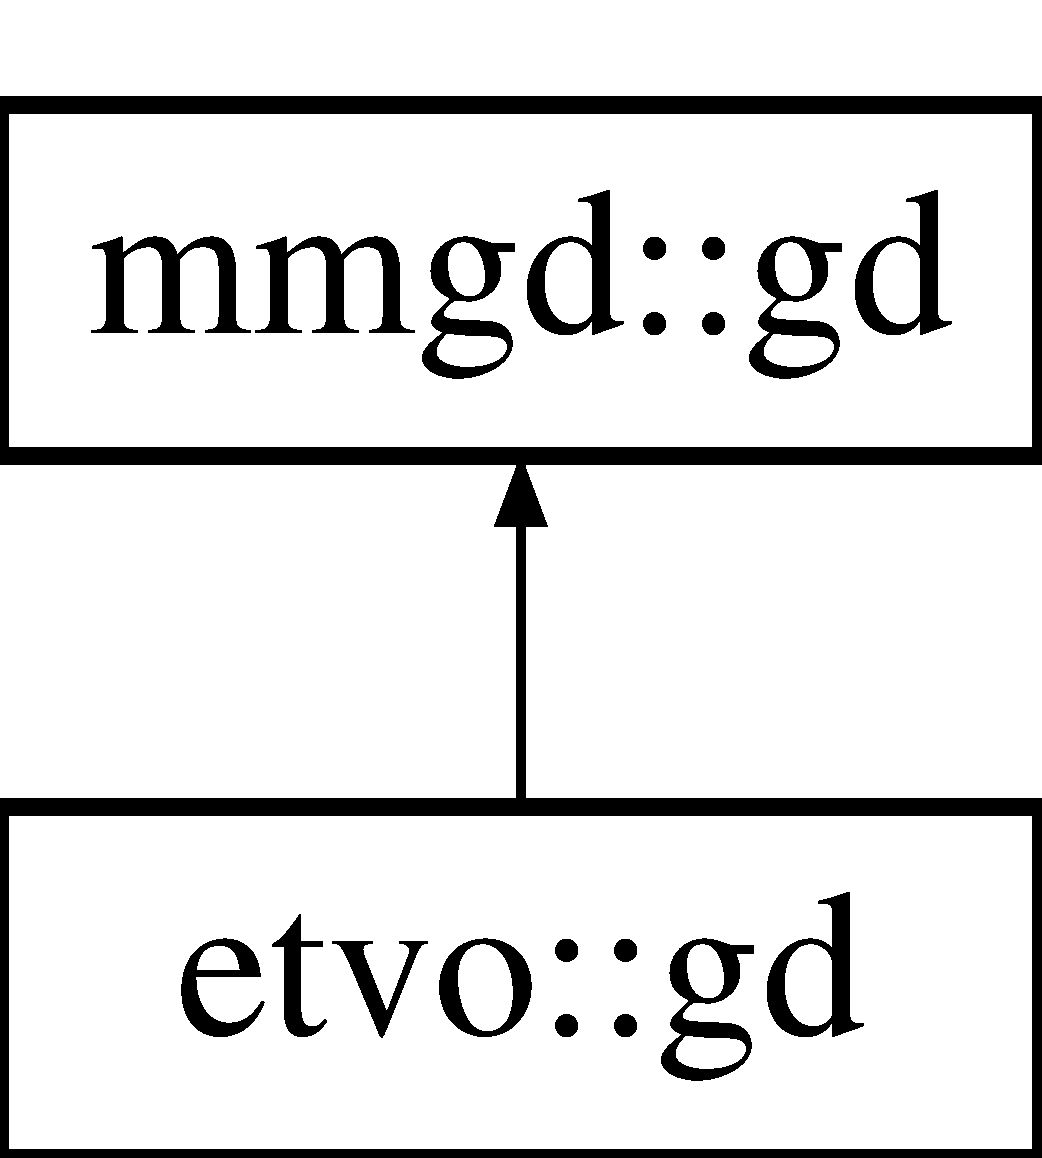
\includegraphics[height=2.000000cm]{classetvo_1_1gd}
\end{center}
\end{figure}
\subsection*{Public Member Functions}
\begin{DoxyCompactItemize}
\item 
\mbox{\label{classetvo_1_1gd_a491fc6a3d50a7a99ec8a1001c94d9f1f}} 
\textbf{ gd} ()
\begin{DoxyCompactList}\small\item\em default constructor \+: set to g$^\wedge$0d$^\wedge$0 \end{DoxyCompactList}\item 
\mbox{\label{classetvo_1_1gd_a3fc5baf5345961b0d6b3ca7c17dd610f}} 
\textbf{ gd} (long g, long d)
\begin{DoxyCompactList}\small\item\em constructor \+: set to g$^\wedge$g.d$^\wedge$d \end{DoxyCompactList}\item 
\mbox{\label{classetvo_1_1gd_aa212987e0ab3679917cafeeb439bcc45}} 
\textbf{ gd} (const \textbf{ gd} \&m)
\begin{DoxyCompactList}\small\item\em copy constructor \end{DoxyCompactList}\item 
\mbox{\label{classetvo_1_1gd_a8418dbde977dfc81a5c240d33e0180cc}} 
\textbf{ gd} (const \textbf{ mmgd\+::gd} \&m)
\begin{DoxyCompactList}\small\item\em construcor \+: set a etvo\+I\+I\+::gd from a \doxyref{mmgd\+::gd}{p.}{classmmgd_1_1gd} \end{DoxyCompactList}\item 
\mbox{\label{classetvo_1_1gd_a69eb1cbc296fb9ab4ab7cf250ea4042b}} 
\textbf{ gd} \& \textbf{ operator=} (const \textbf{ gd} \&m)
\begin{DoxyCompactList}\small\item\em operator=\+: assignation \end{DoxyCompactList}\item 
\mbox{\label{classetvo_1_1gd_ada097f223caef4d58428c8894761af96}} 
\textbf{ gd} \textbf{ operator$\ast$} (const \textbf{ gd} \&m) const
\begin{DoxyCompactList}\small\item\em operator$\ast$\+: product of monomials g$^\wedge$n1d$^\wedge$t1.g$^\wedge$n2d$^\wedge$t2=g$^\wedge$(n1+n2)d$^\wedge$(t1+t2) \end{DoxyCompactList}\item 
\mbox{\label{classetvo_1_1gd_a3d4a0b76fd53360d2dd70dc21605bfe7}} 
long \textbf{ getg} () const
\begin{DoxyCompactList}\small\item\em returns n in g$^\wedge$nd$^\wedge$t \end{DoxyCompactList}\item 
\mbox{\label{classetvo_1_1gd_ae83fea42011af0d4d04e835355f211bd}} 
long \textbf{ getd} () const
\begin{DoxyCompactList}\small\item\em returns t in g$^\wedge$nd$^\wedge$t \end{DoxyCompactList}\item 
\mbox{\label{classetvo_1_1gd_a621d688508a0e6db4e67afc6e45c86f5}} 
bool \textbf{ isE} () const
\begin{DoxyCompactList}\small\item\em check if is equal to g$^\wedge$0d$^\wedge$0 \end{DoxyCompactList}\item 
\mbox{\label{classetvo_1_1gd_affb519d6d467056f5afea9308aea9734}} 
bool \textbf{ is\+Degenerate} () const
\begin{DoxyCompactList}\small\item\em check if n or t are infinite \end{DoxyCompactList}\item 
\mbox{\label{classetvo_1_1gd_ac26ab40728fd575139f84c16410e5b90}} 
bool {\bfseries operator!=} (const \textbf{ gd} \&m) const
\item 
\mbox{\label{classetvo_1_1gd_a34b41726d301dd8250e2b2014c815d0c}} 
bool {\bfseries operator==} (const \textbf{ gd} \&) const
\item 
\mbox{\label{classetvo_1_1gd_a32d371653248425d9984142430004928}} 
bool {\bfseries operator$>$=} (const \textbf{ gd} \&) const
\item 
\mbox{\label{classetvo_1_1gd_a0341db47b2d5e82139b9bb6a3c7cb243}} 
bool {\bfseries operator$<$=} (const \textbf{ gd} \&) const
\item 
\mbox{\label{classetvo_1_1gd_af719cf6c5f35ff62750bd95e04080f82}} 
\textbf{ gd} \textbf{ inf} (const \textbf{ gd} \&m) const
\begin{DoxyCompactList}\small\item\em inf\+: infimum of monomials inf(g$^\wedge$n1d$^\wedge$t1,g$^\wedge$n2d$^\wedge$t2)=g$^\wedge$max(n1,n2)d$^\wedge$min(t1,t2) \end{DoxyCompactList}\item 
\mbox{\label{classetvo_1_1gd_aaa1506c91f51f10b26df53646e4911d0}} 
\textbf{ gd} \textbf{ frac} (const \textbf{ gd} \&m) const
\begin{DoxyCompactList}\small\item\em frac \+: g$^\wedge$n1d$^\wedge$t1/g$^\wedge$n2d$^\wedge$t2 = g$^\wedge$(n1-\/n2)d$^\wedge$(t1-\/t2) \end{DoxyCompactList}\item 
\mbox{\label{classetvo_1_1gd_a2aa893e385df8b963433316142a34e21}} 
\textbf{ poly} \textbf{ operator+} (const \textbf{ gd} \&m) const
\begin{DoxyCompactList}\small\item\em g$^\wedge$n1d$^\wedge$t1 + g$^\wedge$n2d$^\wedge$t2 is a polynomial etvo\+I\+I\+::poly \end{DoxyCompactList}\item 
\mbox{\label{classetvo_1_1gd_a199a8dc018c840489853cfb787f6290a}} 
\textbf{ poly} \textbf{ operator+} (const \textbf{ poly} \&p) const
\begin{DoxyCompactList}\small\item\em g$^\wedge$n1d$^\wedge$t1 + (g$^\wedge$n2d$^\wedge$t2 + ... + g$^\wedge$n\+Kd$^\wedge$tK) is a polynomial \end{DoxyCompactList}\item 
\mbox{\label{classetvo_1_1gd_a18724e0c412c5df4d8374d9d7b996d3e}} 
\textbf{ poly} \textbf{ operator$\ast$} (const \textbf{ poly} \&p) const
\begin{DoxyCompactList}\small\item\em g$^\wedge$n1d$^\wedge$t1 $\ast$ (g$^\wedge$n2d$^\wedge$t2 + ... + g$^\wedge$n\+Kd$^\wedge$tK) is a polynomial \end{DoxyCompactList}\item 
\mbox{\label{classetvo_1_1gd_a56c050b48c34181e209f0b75cea4a1a3}} 
std\+::string \textbf{ To\+String} () const
\begin{DoxyCompactList}\small\item\em returns a string giving the description of a monomial with the format \char`\"{}g2.\+d3\char`\"{} \end{DoxyCompactList}\end{DoxyCompactItemize}
\subsection*{Static Public Member Functions}
\begin{DoxyCompactItemize}
\item 
\mbox{\label{classetvo_1_1gd_a6de3a8b1c425a3ce0bb90b9e7bd46128}} 
static \textbf{ gd} \textbf{ E} ()
\begin{DoxyCompactList}\small\item\em gives the neutral element e=g$^\wedge$0.d$^\wedge$0 \end{DoxyCompactList}\end{DoxyCompactItemize}
\subsection*{Additional Inherited Members}


\subsection{Detailed Description}
Wrapper class to \doxyref{mmgd\+::gd}{p.}{classmmgd_1_1gd} from Min\+Max\+GD library. 

Class for monomials g$^\wedge$n.d$^\wedge$t with finite exponents [n,t finite] In normal cases, no epsilon and no Top elements. But to keep compatible with Min\+Max\+GD, degenerate monomials can be obtained.

\begin{DoxyAuthor}{Author}
BC LH JT L\+A\+R\+IS 
\end{DoxyAuthor}
\begin{DoxyVersion}{Version}
2.\+0 
\end{DoxyVersion}


The documentation for this class was generated from the following files\+:\begin{DoxyCompactItemize}
\item 
F\+:/\+U\+A Box/\+Dev\+Soft/etvo\+I\+I\+I/etvo21/etvo/wrapper\+M\+M\+G\+D/\textbf{ gd\+Wrapper.\+h}\item 
F\+:/\+U\+A Box/\+Dev\+Soft/etvo\+I\+I\+I/etvo21/etvo/wrapper\+M\+M\+G\+D/gd\+Wrapper.\+cpp\end{DoxyCompactItemize}

\section{global Class Reference}
\label{classglobal}\index{global@{global}}
\subsection*{Static Public Attributes}
\begin{DoxyCompactItemize}
\item 
\mbox{\label{classglobal_a9fe6aeb44df54c3e343f6239074246b3}} 
static int {\bfseries L\+I\+M\+I\+T\+\_\+\+T\+R\+A\+N\+S\+\_\+\+D\+E\+L\+TA} = 2000
\item 
\mbox{\label{classglobal_acc4aeb51e1ad5462dab6fce5ed4ce10f}} 
static unsigned {\bfseries N\+B\+\_\+\+I\+T\+ER} = 20
\item 
\mbox{\label{classglobal_a8153f51df56fd7b014bd0bb6474d2d92}} 
static unsigned {\bfseries N\+B\+\_\+\+L\+O\+O\+PS} = 20
\item 
\mbox{\label{classglobal_a745de8daa78fcc2e02d355bcacdb2047}} 
static unsigned char {\bfseries T\+S\+T\+\_\+\+IS} = 1
\item 
\mbox{\label{classglobal_afdd98731166b06015b81324312a983f6}} 
static unsigned char {\bfseries T\+S\+T\+\_\+\+X\+IS} =2
\item 
\mbox{\label{classglobal_a7aea29eb941a586207d32e4c74c5dbc9}} 
static unsigned char {\bfseries T\+S\+T\+\_\+\+R\+E\+S\+I\+D\+U\+EQ} =4
\item 
\mbox{\label{classglobal_aa6d8b94869d802c205cde70e93f34147}} 
static unsigned char {\bfseries T\+S\+T\+\_\+\+R\+E\+S\+I\+D\+U\+I\+N\+EQ} =8
\item 
\mbox{\label{classglobal_a08bdf876f09fa139ae1ce8e6b8225734}} 
static unsigned char {\bfseries T\+S\+T\+\_\+\+A\+LL} =31
\item 
\mbox{\label{classglobal_a5ece81970bfcede24f93054fe77419c4}} 
static unsigned char {\bfseries T\+S\+T\+\_\+\+K\+L\+E\+E\+NE} = 16
\item 
\mbox{\label{classglobal_a0a9a0abc84481a0cb0ddef8f9288ea69}} 
static long {\bfseries I\+NF} = 2147483647
\item 
\mbox{\label{classglobal_a860fb67122fac26af5eb53e82ea07983}} 
static long {\bfseries \+\_\+\+I\+NF} = -\/2147483647
\end{DoxyCompactItemize}


The documentation for this class was generated from the following files\+:\begin{DoxyCompactItemize}
\item 
F\+:/\+U\+A Box/\+Dev\+Soft/etvo\+I\+I\+I/etvo21/etvo/common/global.\+h\item 
F\+:/\+U\+A Box/\+Dev\+Soft/etvo\+I\+I\+I/etvo21/etvo/common/global.\+cpp\end{DoxyCompactItemize}

\section{etvo\+:\+:g\+Ng Class Reference}
\label{classetvo_1_1g_ng}\index{etvo\+::g\+Ng@{etvo\+::g\+Ng}}


Class to describe terms in E[[d]] written g$^\wedge$n.Nabla\+\_\+(m$\vert$b).g$^\wedge$n\textquotesingle{} = g$^\wedge$nl.M\+\_\+m.\+B\+\_\+b.\+g$^\wedge$nr.  




{\ttfamily \#include $<$g\+Ng.\+h$>$}

\subsection*{Public Member Functions}
\begin{DoxyCompactItemize}
\item 
\mbox{\label{classetvo_1_1g_ng_a4df8426135e2185c27f5825a21b6dd9f}} 
\textbf{ g\+Ng} (int nl, unsigned int m, int nc, unsigned int b, int nr)
\begin{DoxyCompactList}\small\item\em Create term g$^\wedge$nl.M\+\_\+m.\+g$^\wedge$nc.B\+\_\+b.\+g$^\wedge$nr. \end{DoxyCompactList}\item 
\mbox{\label{classetvo_1_1g_ng_a81cc8f75787d7c121326be99f46e15e6}} 
\textbf{ g\+Ng} (int nl, unsigned int m, unsigned int b, int nr)
\begin{DoxyCompactList}\small\item\em Create term g$^\wedge$nl.M\+\_\+m.\+g$^\wedge$0.B\+\_\+b.\+g$^\wedge$nr. \end{DoxyCompactList}\item 
\mbox{\label{classetvo_1_1g_ng_a9746007a6d9cda742d3c70ed9d0107bf}} 
\textbf{ g\+Ng} (int nl, unsigned int mb, int nr)
\begin{DoxyCompactList}\small\item\em Create term g$^\wedge$nl.M\+\_\+mb.\+g$^\wedge$0.B\+\_\+mb.\+g$^\wedge$nr. \end{DoxyCompactList}\item 
\mbox{\label{classetvo_1_1g_ng_ad8ff8afadf3f99a47f1344d7f917a313}} 
\textbf{ g\+Ng} (int nc)
\begin{DoxyCompactList}\small\item\em g$^\wedge$0.M\+\_\+1.\+g$^\wedge$nc.B\+\_\+1.\+g$^\wedge$0 = g$^\wedge$nc \end{DoxyCompactList}\item 
int \textbf{ get\+Nl} () const
\item 
\mbox{\label{classetvo_1_1g_ng_ae6a4c801d0ecac9569e6cffca37d7127}} 
unsigned int \textbf{ getM} () const
\begin{DoxyCompactList}\small\item\em getter \+: gives m in g$^\wedge$nl.M\+\_\+m.\+g$^\wedge$nc.B\+\_\+b.\+g$^\wedge$nr \end{DoxyCompactList}\item 
int \textbf{ get\+Nc} () const
\item 
\mbox{\label{classetvo_1_1g_ng_a87e5e422ba7f784920ee5b57833763e1}} 
unsigned int \textbf{ getB} () const
\begin{DoxyCompactList}\small\item\em getter \+: gives b in g$^\wedge$nl.M\+\_\+m.\+g$^\wedge$nc.B\+\_\+b.\+g$^\wedge$nr \end{DoxyCompactList}\item 
int \textbf{ get\+Nr} () const
\item 
\mbox{\label{classetvo_1_1g_ng_ae79b18849ae7585ab1b1e2f3a3611c84}} 
bool {\bfseries operator$<$=} (const \textbf{ g\+Ng} \&m) const
\item 
\mbox{\label{classetvo_1_1g_ng_afa5b3353026093a946e34a8c817f0670}} 
bool {\bfseries operator$>$=} (const \textbf{ g\+Ng} \&m) const
\item 
\mbox{\label{classetvo_1_1g_ng_a84e2c4ab7df598c80bddf5a724bf0813}} 
bool {\bfseries operator==} (const \textbf{ g\+Ng} \&m) const
\item 
\mbox{\label{classetvo_1_1g_ng_aa91e7589ed3dc7d2d614d270a8b0fb2f}} 
void \textbf{ canon} ()
\begin{DoxyCompactList}\small\item\em set to the canonical form (depends on set\+Canon\+Form choice) \end{DoxyCompactList}\item 
\mbox{\label{classetvo_1_1g_ng_abbc92a58a717475ea5428694e14b06bb}} 
void \textbf{ canonL} ()
\begin{DoxyCompactList}\small\item\em set to the Left form [0$<$=nr$<$=b-\/1 and nc=0] \end{DoxyCompactList}\item 
\mbox{\label{classetvo_1_1g_ng_a59b42fff71fe9e8441abe8b34817da6b}} 
void \textbf{ canonC} ()
\begin{DoxyCompactList}\small\item\em set to the Central [0$<$=nl$<$=m-\/1 and 0$<$=nr$<$=b-\/1] \end{DoxyCompactList}\item 
\mbox{\label{classetvo_1_1g_ng_aa884c2eee0684e2f9b799391cdf3cae0}} 
void \textbf{ canonR} ()
\begin{DoxyCompactList}\small\item\em set to the Right form [0$<$=nl$<$=m-\/1 and nc=0] \end{DoxyCompactList}\item 
\mbox{\label{classetvo_1_1g_ng_a2e553fda308f55dc03b72e01beff9ba7}} 
int \textbf{ Fw} (int ki) const
\begin{DoxyCompactList}\small\item\em value of C/C function Fw(ki) = floor(((nr+ki)/b)+nc)$\ast$m+nl \end{DoxyCompactList}\item 
\mbox{\label{classetvo_1_1g_ng_aaef675c29f18dbda395d564c066bde02}} 
\textbf{ Fminp} \textbf{ get\+Fw} () const
\begin{DoxyCompactList}\small\item\em returns function Fw as a \doxyref{Fminp}{p.}{classetvo_1_1_fminp} object \end{DoxyCompactList}\item 
\mbox{\label{classetvo_1_1g_ng_af9e4a33cf4778c7ac75a096141b7b3b9}} 
\textbf{ E\+\_\+op} \textbf{ extend\+By} (unsigned mul) const
\begin{DoxyCompactList}\small\item\em Extension of g$^\wedge$nl M\+\_\+m B\+\_\+b g$^\wedge$nr -\/$>$ S\+U\+M\+\_\+i g$^\wedge$(nl+i$\ast$ M\+\_\+(mul$\ast$m) B\+\_\+(mul$\ast$\+\_\+b) g$^\wedge$(mul-\/1) .... \end{DoxyCompactList}\item 
\mbox{\label{classetvo_1_1g_ng_a7fa5aad64177680647485bff30661d7b}} 
std\+::pair$<$ unsigned, unsigned $>$ \textbf{ get\+Periodicity} () const
\begin{DoxyCompactList}\small\item\em returns periodicity as a pair $<$\+\_\+b,\+\_\+m$>$ \end{DoxyCompactList}\item 
std\+::string \textbf{ to\+String} (unsigned n\+Ver=0) const
\end{DoxyCompactItemize}
\subsection*{Static Public Member Functions}
\begin{DoxyCompactItemize}
\item 
static void \textbf{ set\+Canon\+Form} (unsigned val=0)
\item 
\mbox{\label{classetvo_1_1g_ng_a5943a784420a1d37346c80e91d2762ee}} 
static unsigned {\bfseries get\+Canon\+Form} ()
\end{DoxyCompactItemize}
\subsection*{Protected Attributes}
\begin{DoxyCompactItemize}
\item 
\mbox{\label{classetvo_1_1g_ng_ad143fd48763e3d41765391b3fcde64e1}} 
int \textbf{ \+\_\+nl}
\begin{DoxyCompactList}\small\item\em nl,m,b,nr \end{DoxyCompactList}\item 
\mbox{\label{classetvo_1_1g_ng_a4934cf8a9b2fba6df1173e560ede3b40}} 
unsigned int {\bfseries \+\_\+m}
\item 
\mbox{\label{classetvo_1_1g_ng_a3a4bbf59c0f5042901c9cd2ce0c19b71}} 
int {\bfseries \+\_\+nc}
\item 
\mbox{\label{classetvo_1_1g_ng_ac4fba04953e3fe0e4e46f3822601e9a7}} 
unsigned int {\bfseries \+\_\+b}
\item 
\mbox{\label{classetvo_1_1g_ng_aa2e659eea1a7eef34bcbbf708e7888af}} 
int {\bfseries \+\_\+nr}
\end{DoxyCompactItemize}
\subsection*{Static Protected Attributes}
\begin{DoxyCompactItemize}
\item 
static unsigned \textbf{ \+\_\+canon} =0
\begin{DoxyCompactList}\small\item\em set the canonical form of \doxyref{g\+Ng}{p.}{classetvo_1_1g_ng} (default left form) \end{DoxyCompactList}\end{DoxyCompactItemize}


\subsection{Detailed Description}
Class to describe terms in E[[d]] written g$^\wedge$n.Nabla\+\_\+(m$\vert$b).g$^\wedge$n\textquotesingle{} = g$^\wedge$nl.M\+\_\+m.\+B\+\_\+b.\+g$^\wedge$nr. 

Formal series in E[[d]] can be seen as infinite sums of terms (g$^\wedge$nli.M\+\_\+m.\+B\+\_\+b.\+g$^\wedge$nri).d$^\wedge$t\+\_\+i

We can also decompose a \doxyref{g\+Ng}{p.}{classetvo_1_1g_ng} term into a central form (g$^\wedge$nli.M\+\_\+m.\+g$^\wedge$nci.B\+\_\+b.\+g$^\wedge$nri) where nli$<$m and nri$<$b

\begin{DoxyAuthor}{Author}
BC LH JT L\+A\+R\+IS 
\end{DoxyAuthor}
\begin{DoxyVersion}{Version}
2.\+0 
\end{DoxyVersion}


\subsection{Member Function Documentation}
\mbox{\label{classetvo_1_1g_ng_ae0a9274b983c28603f376285906216f0}} 
\index{etvo\+::g\+Ng@{etvo\+::g\+Ng}!get\+Nc@{get\+Nc}}
\index{get\+Nc@{get\+Nc}!etvo\+::g\+Ng@{etvo\+::g\+Ng}}
\subsubsection{get\+Nc()}
{\footnotesize\ttfamily int etvo\+::g\+Ng\+::get\+Nc (\begin{DoxyParamCaption}{ }\end{DoxyParamCaption}) const}

getter \+: gives nc in g$^\wedge$nl.M\+\_\+m.\+g$^\wedge$nc.B\+\_\+b.\+g$^\wedge$nr depends on the chosen form (it is 0 in left and right form) \mbox{\label{classetvo_1_1g_ng_aa973f873c83f4c23c7c781597f21300b}} 
\index{etvo\+::g\+Ng@{etvo\+::g\+Ng}!get\+Nl@{get\+Nl}}
\index{get\+Nl@{get\+Nl}!etvo\+::g\+Ng@{etvo\+::g\+Ng}}
\subsubsection{get\+Nl()}
{\footnotesize\ttfamily int etvo\+::g\+Ng\+::get\+Nl (\begin{DoxyParamCaption}{ }\end{DoxyParamCaption}) const}

getter \+: gives nl in g$^\wedge$nl.M\+\_\+m.\+g$^\wedge$nc.B\+\_\+b.\+g$^\wedge$nr depends on the chosen form \mbox{\label{classetvo_1_1g_ng_afc55d8833496cdc23c0365bfb97e638a}} 
\index{etvo\+::g\+Ng@{etvo\+::g\+Ng}!get\+Nr@{get\+Nr}}
\index{get\+Nr@{get\+Nr}!etvo\+::g\+Ng@{etvo\+::g\+Ng}}
\subsubsection{get\+Nr()}
{\footnotesize\ttfamily int etvo\+::g\+Ng\+::get\+Nr (\begin{DoxyParamCaption}{ }\end{DoxyParamCaption}) const}

getter \+: gives nc in g$^\wedge$nl.M\+\_\+m.\+g$^\wedge$nc.B\+\_\+b.\+g$^\wedge$nr depends on the chosen form \mbox{\label{classetvo_1_1g_ng_a7baa5b43ab27486ed13329b26626c7ef}} 
\index{etvo\+::g\+Ng@{etvo\+::g\+Ng}!set\+Canon\+Form@{set\+Canon\+Form}}
\index{set\+Canon\+Form@{set\+Canon\+Form}!etvo\+::g\+Ng@{etvo\+::g\+Ng}}
\subsubsection{set\+Canon\+Form()}
{\footnotesize\ttfamily void etvo\+::g\+Ng\+::set\+Canon\+Form (\begin{DoxyParamCaption}\item[{unsigned}]{val = {\ttfamily 0} }\end{DoxyParamCaption})\hspace{0.3cm}{\ttfamily [static]}}

Class method to choose the canonical form of \doxyref{g\+Ng}{p.}{classetvo_1_1g_ng} terms


\begin{DoxyParams}{Parameters}
{\em val=0-\/left} & form 1-\/central form 2-\/ right form \\
\hline
\end{DoxyParams}
\mbox{\label{classetvo_1_1g_ng_a87bd5315939b1792c48a459b464c96ff}} 
\index{etvo\+::g\+Ng@{etvo\+::g\+Ng}!to\+String@{to\+String}}
\index{to\+String@{to\+String}!etvo\+::g\+Ng@{etvo\+::g\+Ng}}
\subsubsection{to\+String()}
{\footnotesize\ttfamily std\+::string etvo\+::g\+Ng\+::to\+String (\begin{DoxyParamCaption}\item[{unsigned}]{n\+Ver = {\ttfamily 0} }\end{DoxyParamCaption}) const}

gives a string description of a \doxyref{g\+Ng}{p.}{classetvo_1_1g_ng} term 
\begin{DoxyParams}{Parameters}
{\em n\+Ver} & (default=0) ~\newline
 if n\+Ver=0 -\/$>$ produces string \char`\"{}g-\/3.\+m3.\+b4.\+g4\char`\"{} ~\newline
if n\+Ver!=0 -\/$>$ only for development \\
\hline
\end{DoxyParams}


\subsection{Member Data Documentation}
\mbox{\label{classetvo_1_1g_ng_a5cf9a7b5b14be4afe30b9aff675cf99e}} 
\index{etvo\+::g\+Ng@{etvo\+::g\+Ng}!\+\_\+canon@{\+\_\+canon}}
\index{\+\_\+canon@{\+\_\+canon}!etvo\+::g\+Ng@{etvo\+::g\+Ng}}
\subsubsection{\+\_\+canon}
{\footnotesize\ttfamily unsigned etvo\+::g\+Ng\+::\+\_\+canon =0\hspace{0.3cm}{\ttfamily [static]}, {\ttfamily [protected]}}



set the canonical form of \doxyref{g\+Ng}{p.}{classetvo_1_1g_ng} (default left form) 

set the default form (=0) as Left Form 

The documentation for this class was generated from the following files\+:\begin{DoxyCompactItemize}
\item 
F\+:/\+U\+A Box/\+Dev\+Soft/etvo\+I\+I\+I/etvo21/etvo/etop/\textbf{ g\+Ng.\+h}\item 
F\+:/\+U\+A Box/\+Dev\+Soft/etvo\+I\+I\+I/etvo21/etvo/etop/g\+Ng.\+cpp\end{DoxyCompactItemize}

\section{etvo\+:\+:I\+Sterm Class Reference}
\label{classetvo_1_1_i_sterm}\index{etvo\+::\+I\+Sterm@{etvo\+::\+I\+Sterm}}


Abstract base class to handle Idempotent Semiring terms.  




{\ttfamily \#include $<$I\+Sterm.\+h$>$}

Inheritance diagram for etvo\+:\+:I\+Sterm\+:\begin{figure}[H]
\begin{center}
\leavevmode
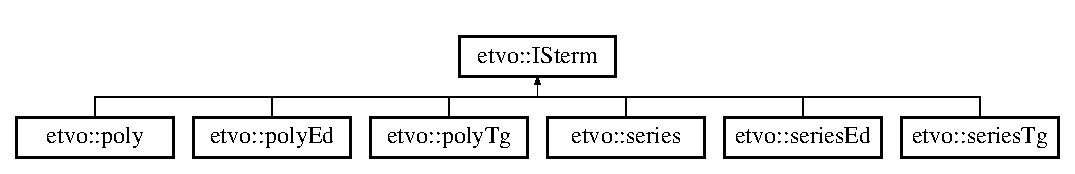
\includegraphics[height=1.885522cm]{classetvo_1_1_i_sterm}
\end{center}
\end{figure}
\subsection*{Public Member Functions}
\begin{DoxyCompactItemize}
\item 
\mbox{\label{classetvo_1_1_i_sterm_a2770f7090dc44b664773bae24cb3fa16}} 
\textbf{ I\+Sterm} (bool is\+Epsilon=false)
\begin{DoxyCompactList}\small\item\em default constructor \+: an epsilon term \end{DoxyCompactList}\item 
\mbox{\label{classetvo_1_1_i_sterm_acdcfe8c39b5783fc891373fe9ebfba03}} 
\textbf{ I\+Sterm} (int eps\+N\+Top)
\begin{DoxyCompactList}\small\item\em constructor to specify the type of \doxyref{I\+Sterm}{p.}{classetvo_1_1_i_sterm} \end{DoxyCompactList}\item 
\mbox{\label{classetvo_1_1_i_sterm_a6ed12700e35a84ef3a6bf852433882db}} 
bool {\bfseries is\+Epsilon} () const
\item 
\mbox{\label{classetvo_1_1_i_sterm_ae721e3fa0f1f6f2bd36b1793caabfd22}} 
bool {\bfseries is\+Top} () const
\item 
\mbox{\label{classetvo_1_1_i_sterm_ad457132ac788ddd78be3bd909345427c}} 
bool {\bfseries is\+Extreme} () const
\item 
\mbox{\label{classetvo_1_1_i_sterm_a3fa1ae37666661f7dec558fa198dd8da}} 
void {\bfseries set\+Epsilon} ()
\item 
\mbox{\label{classetvo_1_1_i_sterm_ae8b288b60a7f9c5c5c1597f337127c9d}} 
void {\bfseries set\+Top} ()
\item 
\mbox{\label{classetvo_1_1_i_sterm_a11e93913bcde5123734974cf3930cb00}} 
bool {\bfseries operator==} (const \textbf{ I\+Sterm} \&) const
\end{DoxyCompactItemize}
\subsection*{Protected Attributes}
\begin{DoxyCompactItemize}
\item 
\mbox{\label{classetvo_1_1_i_sterm_a04eb25dbdba96268cffe6a80bb6b029b}} 
char \textbf{ \+\_\+eps\+N\+Top}
\begin{DoxyCompactList}\small\item\em \+\_\+eps\+N\+Top = -\/1 epsilon 0 not extrem (normal) +1 Top \end{DoxyCompactList}\end{DoxyCompactItemize}


\subsection{Detailed Description}
Abstract base class to handle Idempotent Semiring terms. 

Attribute \+\_\+eps\+N\+Top describes epsilon (-\/1) Top(+1) and Not extrem (0)

\begin{DoxyAuthor}{Author}
BC LH JT L\+A\+R\+IS 
\end{DoxyAuthor}
\begin{DoxyVersion}{Version}
2.\+0 
\end{DoxyVersion}


The documentation for this class was generated from the following files\+:\begin{DoxyCompactItemize}
\item 
F\+:/\+U\+A Box/\+Dev\+Soft/etvo\+I\+I\+I/etvo21/etvo/common/\textbf{ I\+Sterm.\+h}\item 
F\+:/\+U\+A Box/\+Dev\+Soft/etvo\+I\+I\+I/etvo21/etvo/common/I\+Sterm.\+cpp\end{DoxyCompactItemize}

\section{etvo\+:\+:matrix$<$ T $>$ Class Template Reference}
\label{classetvo_1_1matrix}\index{etvo\+::matrix$<$ T $>$@{etvo\+::matrix$<$ T $>$}}
\subsection*{Public Member Functions}
\begin{DoxyCompactItemize}
\item 
\mbox{\label{classetvo_1_1matrix_a652c87888b7f22683326a920d20ce885}} 
{\bfseries operator T} ()
\item 
\mbox{\label{classetvo_1_1matrix_a2053769b66ded9534706ed384ad1aacf}} 
\textbf{ matrix} (unsigned li=1, unsigned co=1)
\begin{DoxyCompactList}\small\item\em Initialize a matrix of size li x co. \end{DoxyCompactList}\item 
\mbox{\label{classetvo_1_1matrix_a2906428c7c4695a34104d92ef6b873bf}} 
T \& \textbf{ operator()} (unsigned li, unsigned co)
\begin{DoxyCompactList}\small\item\em returns the entry (li,co) \end{DoxyCompactList}\item 
\mbox{\label{classetvo_1_1matrix_a50b4a1ad335afa30198321c7d870a8ce}} 
T \textbf{ operator()} (unsigned li, unsigned co) const
\begin{DoxyCompactList}\small\item\em returns the entry (li,co) \end{DoxyCompactList}\item 
\mbox{\label{classetvo_1_1matrix_a4d550808aec3aaf2faea4eb1e0d9975a}} 
\textbf{ matrix}$<$ T $>$ \textbf{ operator+} (const \textbf{ matrix}$<$ T $>$ \&mat) const
\begin{DoxyCompactList}\small\item\em returns the sum of two matrices (with the + rule from T) \end{DoxyCompactList}\item 
\mbox{\label{classetvo_1_1matrix_a7d267f72949f2cdd73b23520ced84782}} 
\textbf{ matrix}$<$ T $>$ \textbf{ operator$\ast$} (const \textbf{ matrix}$<$ T $>$ \&mat) const
\begin{DoxyCompactList}\small\item\em returns the product of two matrices (with the $\ast$ rule from T) \end{DoxyCompactList}\item 
\mbox{\label{classetvo_1_1matrix_a8820833053792ecd3d862d73576bb90d}} 
\textbf{ matrix}$<$ T $>$ \textbf{ lfrac} (const \textbf{ matrix}$<$ T $>$ \&mat) const
\begin{DoxyCompactList}\small\item\em returns the left product residuation of two matrices \end{DoxyCompactList}\item 
\mbox{\label{classetvo_1_1matrix_ae2b16ea0cc5279487975257aee47a545}} 
\textbf{ matrix}$<$ T $>$ \textbf{ rfrac} (const \textbf{ matrix}$<$ T $>$ \&mat) const
\begin{DoxyCompactList}\small\item\em returns the right product residuation of two matrices \end{DoxyCompactList}\item 
\mbox{\label{classetvo_1_1matrix_ac2189677830feabc6e308a5d9bf22817}} 
\textbf{ matrix}$<$ T $>$ \textbf{ inf} (const \textbf{ matrix}$<$ T $>$ \&mat) const
\begin{DoxyCompactList}\small\item\em returns the infimum of two matrices (with the rule from T) \end{DoxyCompactList}\item 
\mbox{\label{classetvo_1_1matrix_ae56483bd216936c4b617f37442d03957}} 
\textbf{ matrix}$<$ T $>$ \textbf{ star} () const
\begin{DoxyCompactList}\small\item\em returns the Kleene star of the current matrix \end{DoxyCompactList}\item 
\mbox{\label{classetvo_1_1matrix_a7b5aefcfde4dc4f2c8ac474979f818ec}} 
unsigned int \textbf{ Get\+Row} () const
\begin{DoxyCompactList}\small\item\em returns the number of rows \end{DoxyCompactList}\item 
\mbox{\label{classetvo_1_1matrix_ae584b7f3d692303116a953a0f006fd18}} 
unsigned int \textbf{ Get\+Column} () const
\begin{DoxyCompactList}\small\item\em returns the number of columns \end{DoxyCompactList}\item 
\mbox{\label{classetvo_1_1matrix_a45eb3ce5be46f7b41ae4572d7dd0462e}} 
bool \textbf{ operator==} (const \textbf{ matrix}$<$ T $>$ \&m) const
\begin{DoxyCompactList}\small\item\em checks equality \end{DoxyCompactList}\end{DoxyCompactItemize}


The documentation for this class was generated from the following file\+:\begin{DoxyCompactItemize}
\item 
F\+:/\+U\+A Box/\+Dev\+Soft/etvo\+I\+I\+I/etvo21/etvo/wrapper\+M\+M\+G\+D/\textbf{ matrix\+Wrapper.\+h}\end{DoxyCompactItemize}

\section{etvo\+:\+:matrix$<$ T $>$ Class Reference}
\label{classetvo_1_1matrix_3_01_t_01_4}\index{etvo\+::matrix$<$ T $>$@{etvo\+::matrix$<$ T $>$}}


Template class to create matrix of semiring elements (series,\doxyref{series\+Ed}{p.}{classetvo_1_1series_ed} ...)  




{\ttfamily \#include $<$matrix\+Wrapper.\+h$>$}



\subsection{Detailed Description}
Template class to create matrix of semiring elements (series,\doxyref{series\+Ed}{p.}{classetvo_1_1series_ed} ...) 

\begin{DoxyAuthor}{Author}
BC LH JT L\+A\+R\+IS 
\end{DoxyAuthor}
\begin{DoxyVersion}{Version}
2.\+0 
\end{DoxyVersion}


The documentation for this class was generated from the following file\+:\begin{DoxyCompactItemize}
\item 
F\+:/\+U\+A Box/\+Dev\+Soft/etvo\+I\+I\+I/etvo21/etvo/wrapper\+M\+M\+G\+D/\textbf{ matrix\+Wrapper.\+h}\end{DoxyCompactItemize}

\section{mmgd\+:\+:mmgd\+:\+:mem\+\_\+limite Class Reference}
\label{classmmgd_1_1mmgd_1_1mem__limite}\index{mmgd\+::mmgd\+::mem\+\_\+limite@{mmgd\+::mmgd\+::mem\+\_\+limite}}
\subsection*{Public Member Functions}
\begin{DoxyCompactItemize}
\item 
\mbox{\label{classmmgd_1_1mmgd_1_1mem__limite_aad2cbbb4c4badf1603cf5df569f6e9d3}} 
{\bfseries mem\+\_\+limite} (int i)
\end{DoxyCompactItemize}
\subsection*{Public Attributes}
\begin{DoxyCompactItemize}
\item 
\mbox{\label{classmmgd_1_1mmgd_1_1mem__limite_a3593e1dfa0fba70fd228277b9343c212}} 
int {\bfseries memoire}
\end{DoxyCompactItemize}


The documentation for this class was generated from the following file\+:\begin{DoxyCompactItemize}
\item 
F\+:/\+U\+A Box/\+Dev\+Soft/etvo\+I\+I\+I/etvo21/etvo/libminmaxgd/src/poly.\+cpp\end{DoxyCompactItemize}

\section{mmgd\+:\+:mem\+\_\+limite Class Reference}
\label{classmmgd_1_1mem__limite}\index{mmgd\+::mem\+\_\+limite@{mmgd\+::mem\+\_\+limite}}
\subsection*{Public Member Functions}
\begin{DoxyCompactItemize}
\item 
\mbox{\label{classmmgd_1_1mem__limite_ab00a238d0429a5bf079c4534db8b912c}} 
{\bfseries mem\+\_\+limite} (int i)
\end{DoxyCompactItemize}
\subsection*{Public Attributes}
\begin{DoxyCompactItemize}
\item 
\mbox{\label{classmmgd_1_1mem__limite_ade5cb5c82021ac0faaf831ab83ece8ae}} 
int {\bfseries memoire}
\end{DoxyCompactItemize}


The documentation for this class was generated from the following file\+:\begin{DoxyCompactItemize}
\item 
F\+:/\+U\+A Box/\+Dev\+Soft/etvo\+I\+I\+I/etvo21/etvo/libminmaxgd/include/gd.\+h\end{DoxyCompactItemize}

\section{graphic\+PR\+:\+:Pov\+Ray\+:\+:Point Class Reference}
\label{classgraphic_p_r_1_1_pov_ray_1_1_point}\index{graphic\+P\+R\+::\+Pov\+Ray\+::\+Point@{graphic\+P\+R\+::\+Pov\+Ray\+::\+Point}}


the script description of a point in P\+O\+V-\/\+Ray  




{\ttfamily \#include $<$Pov\+Ray.\+h$>$}

\subsection*{Public Member Functions}
\begin{DoxyCompactItemize}
\item 
\mbox{\label{classgraphic_p_r_1_1_pov_ray_1_1_point_af2b101fab017a294414e04b37479ff2e}} 
{\bfseries Point} (float X=0, float Y=0, float Z=0)
\item 
\mbox{\label{classgraphic_p_r_1_1_pov_ray_1_1_point_a2a1ba72e55e03b5077137f5a87e7263d}} 
std\+::string {\bfseries To\+String} () const
\end{DoxyCompactItemize}
\subsection*{Public Attributes}
\begin{DoxyCompactItemize}
\item 
\mbox{\label{classgraphic_p_r_1_1_pov_ray_1_1_point_a5cbe3f90db8c633df58d56d0d1bbeb4b}} 
float {\bfseries x}
\item 
\mbox{\label{classgraphic_p_r_1_1_pov_ray_1_1_point_ac4fff265720fdf38b167a9591421f8b6}} 
float {\bfseries y}
\item 
\mbox{\label{classgraphic_p_r_1_1_pov_ray_1_1_point_ae268260b962a44f8d9cf518bbb877247}} 
float {\bfseries z}
\end{DoxyCompactItemize}


\subsection{Detailed Description}
the script description of a point in P\+O\+V-\/\+Ray 

The documentation for this class was generated from the following file\+:\begin{DoxyCompactItemize}
\item 
F\+:/\+U\+A Box/\+Dev\+Soft/etvo\+I\+I\+I/etvo21/etvo/grafic/Pov\+Ray.\+h\end{DoxyCompactItemize}

\section{etvo\+:\+:poly Class Reference}
\label{classetvo_1_1poly}\index{etvo\+::poly@{etvo\+::poly}}


Wrapper class to \doxyref{mmgd\+::poly}{p.}{classmmgd_1_1poly} from from Min\+Max\+GD library.  




{\ttfamily \#include $<$poly\+Wrapper.\+h$>$}

Inheritance diagram for etvo\+:\+:poly\+:\begin{figure}[H]
\begin{center}
\leavevmode
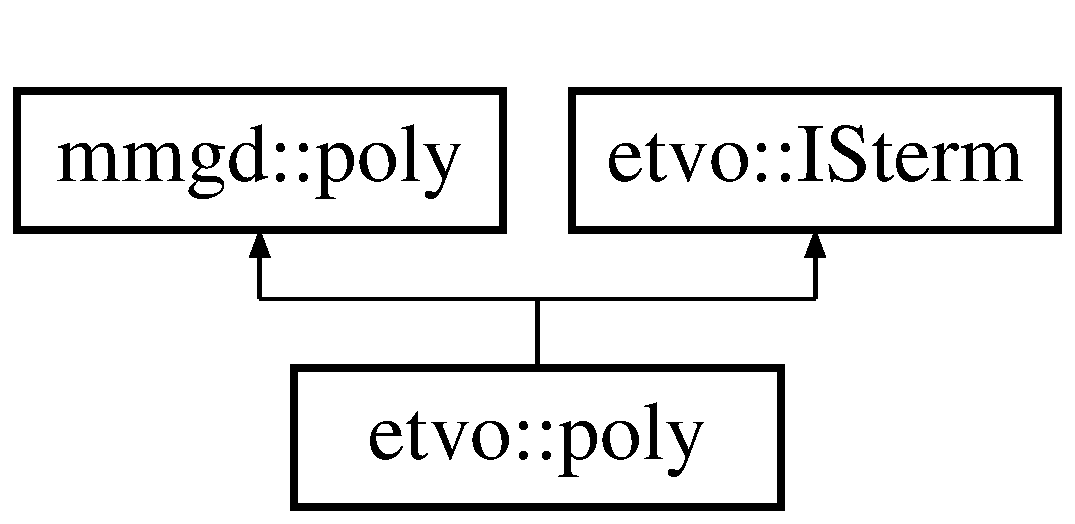
\includegraphics[height=2.000000cm]{classetvo_1_1poly}
\end{center}
\end{figure}
\subsection*{Public Member Functions}
\begin{DoxyCompactItemize}
\item 
\mbox{\label{classetvo_1_1poly_a6c6583c015d418232464d7e807de1093}} 
bool \textbf{ is\+Epsilon} () const
\begin{DoxyCompactList}\small\item\em check if it is equal to epsilon \end{DoxyCompactList}\item 
\mbox{\label{classetvo_1_1poly_afb10e05c72e24072195eea59b356c8e7}} 
bool \textbf{ isE} () const
\begin{DoxyCompactList}\small\item\em check if it is equal to e \end{DoxyCompactList}\item 
\mbox{\label{classetvo_1_1poly_a08433bd25884d1614e6995a8ca239d0c}} 
bool \textbf{ is\+Degenerate} () const
\begin{DoxyCompactList}\small\item\em check if it is degenrate (at least one degenrate monomial) \end{DoxyCompactList}\item 
\mbox{\label{classetvo_1_1poly_ae71bb69910720ebda2718ed203e0fdab}} 
\textbf{ poly} ()
\begin{DoxyCompactList}\small\item\em default constructor = epsilon polynomial \end{DoxyCompactList}\item 
\mbox{\label{classetvo_1_1poly_a9a1774bdb443aefc2708744a6617f447}} 
\textbf{ poly} (bool Top\+NotE)
\begin{DoxyCompactList}\small\item\em constructor Top or E polynomial \+: if Top\+NotE=true -\/$>$ Top else -\/$>$ g$^\wedge$0.d$^\wedge$0 \end{DoxyCompactList}\item 
\mbox{\label{classetvo_1_1poly_aef1b43f4218fad601d608d3c122f389a}} 
\textbf{ poly} (const \textbf{ gd} \&m)
\begin{DoxyCompactList}\small\item\em constructor \+: a polynomial with only one monomial p=g$^\wedge$n.d$^\wedge$t \end{DoxyCompactList}\item 
\mbox{\label{classetvo_1_1poly_a986cb9fecfee314838479524ce129aa0}} 
\textbf{ poly} (const \textbf{ mmgd\+::poly} \&p)
\begin{DoxyCompactList}\small\item\em constructor \+: a polynomial set from a \doxyref{mmgd\+::poly}{p.}{classmmgd_1_1poly} object \end{DoxyCompactList}\item 
\mbox{\label{classetvo_1_1poly_ad950b2b645d5f29659825b71539c110a}} 
\textbf{ poly} (long n, long t)
\begin{DoxyCompactList}\small\item\em constructor \+: a polynomial with only one monomial p=g$^\wedge$n.d$^\wedge$t \end{DoxyCompactList}\item 
\mbox{\label{classetvo_1_1poly_adcf452b6db20e58db518edaaa9bd5e4e}} 
\textbf{ poly} (const std\+::vector$<$ \textbf{ mmgd\+::gd} $>$ \&v)
\begin{DoxyCompactList}\small\item\em constructor\+: set a polynomial initialized from a collection of monomials. The polynomial p=Sum\+\_\+i g$^\wedge$nid$^\wedge$ti is set in a standard form where ni$<$ni+1 ti$<$ti+1 \end{DoxyCompactList}\item 
\mbox{\label{classetvo_1_1poly_add4e82b9ada5e47b517ce428db997e25}} 
\textbf{ poly} (const std\+::vector$<$ \textbf{ gd} $>$ \&v)
\begin{DoxyCompactList}\small\item\em constructor\+: a polynomial initialized from a collection of monomials. The polynomial p=Sum\+\_\+i g$^\wedge$nid$^\wedge$ti is set in a standard form where ni$<$ni+1 ti$<$ti+1 \end{DoxyCompactList}\item 
\mbox{\label{classetvo_1_1poly_a064c6143d96c29bdb3fadc0b895ab9c3}} 
void \textbf{ add} (const \textbf{ gd} \&m)
\begin{DoxyCompactList}\small\item\em adds a new monomial to the current polynomial, but simplification does not operate. Then, the current polynomial is no longer in standard form. \end{DoxyCompactList}\item 
\mbox{\label{classetvo_1_1poly_ae90e648838663b4c640e888991bd2f7c}} 
unsigned \textbf{ size} () const
\begin{DoxyCompactList}\small\item\em returns the number of monomials \end{DoxyCompactList}\item 
\mbox{\label{classetvo_1_1poly_a7d1351632a661242e08ca6329a53035e}} 
\textbf{ gd} \textbf{ operator[$\,$]} (unsigned i) const
\begin{DoxyCompactList}\small\item\em returns a copy of one of the monomials (modification is not allowed) \end{DoxyCompactList}\item 
\mbox{\label{classetvo_1_1poly_a064c2b912a9975fb744c886f078d8a79}} 
\textbf{ poly} \& \textbf{ operator=} (const \textbf{ poly} \&p)
\begin{DoxyCompactList}\small\item\em operator = assignment \end{DoxyCompactList}\item 
\mbox{\label{classetvo_1_1poly_a4b71b767fa8f4a2a7e9e654703e4ec18}} 
\textbf{ poly} \& \textbf{ operator=} (const \textbf{ gd} \&m)
\begin{DoxyCompactList}\small\item\em operator = assignment \end{DoxyCompactList}\item 
\mbox{\label{classetvo_1_1poly_a917cd79ff92d6a07bdfb36dd9fa01b40}} 
bool \textbf{ operator==} (const \textbf{ poly} \&p) const
\begin{DoxyCompactList}\small\item\em operator== checks equality \end{DoxyCompactList}\item 
\mbox{\label{classetvo_1_1poly_ab14522cf65b1c44292bf88ecf21f0e11}} 
bool {\bfseries operator!=} (const \textbf{ poly} \&p) const
\item 
\mbox{\label{classetvo_1_1poly_a3a76de2e1704d2970faa4294ec3dab61}} 
bool \textbf{ operator$<$=} (const \textbf{ poly} \&p) const
\begin{DoxyCompactList}\small\item\em operator$<$= order according to the Min\+Max[[g,d]] rule \end{DoxyCompactList}\item 
\mbox{\label{classetvo_1_1poly_af58ba8cdedb436a07b7b76df9f26f764}} 
bool \textbf{ operator$>$=} (const \textbf{ poly} \&p) const
\begin{DoxyCompactList}\small\item\em operator$<$= order according to the Min\+Max[[g,d]] rule \end{DoxyCompactList}\item 
\mbox{\label{classetvo_1_1poly_a36e74ff109f7d749e07a528b1ef4babe}} 
\textbf{ poly} \textbf{ operator+} (const \textbf{ poly} \&p) const
\begin{DoxyCompactList}\small\item\em operator+ sum of polynomials p1+p2 is a polynomial \end{DoxyCompactList}\item 
\mbox{\label{classetvo_1_1poly_aa40dc038b238731b2d0cf5c8af15ccb8}} 
\textbf{ poly} \textbf{ operator+} (const \textbf{ gd} \&m) const
\begin{DoxyCompactList}\small\item\em operator+ sum of a polynomial with a monomial p+m is a polynomial \end{DoxyCompactList}\item 
\mbox{\label{classetvo_1_1poly_a5988155bfd5c1fa490d7b13954d40640}} 
\textbf{ poly} \textbf{ operator$\ast$} (const \textbf{ poly} \&p) const
\begin{DoxyCompactList}\small\item\em operator$\ast$ product of polynomials p1$\ast$p2 is a polynomial \end{DoxyCompactList}\item 
\mbox{\label{classetvo_1_1poly_a995e766e7dca089dd51d2542a0f381fc}} 
\textbf{ poly} \textbf{ operator$\ast$} (const \textbf{ gd} \&m) const
\begin{DoxyCompactList}\small\item\em operator$\ast$ product of a polynomial and a monomial p$\ast$m is a polynomial \end{DoxyCompactList}\item 
\mbox{\label{classetvo_1_1poly_a8e5ad29d9c2b39a92918cb997ca765b6}} 
\textbf{ poly} \textbf{ inf} (const \textbf{ poly} \&p) const
\begin{DoxyCompactList}\small\item\em infimum of two polynomials p1.\+inf(p2)=greatest p s.\+t. p$<$=p1 and p$<$=p2 \end{DoxyCompactList}\item 
\mbox{\label{classetvo_1_1poly_aad781953b85beb88494f2cc56d921f16}} 
\textbf{ poly} \textbf{ inf} (const \textbf{ gd} \&m) const
\begin{DoxyCompactList}\small\item\em infimum p1.\+inf(m)=greatest p s.\+t. p$<$=p1 and p$<$=m \end{DoxyCompactList}\item 
\mbox{\label{classetvo_1_1poly_a4c5250c9926e38ef547c3298c385a994}} 
\textbf{ poly} \textbf{ lfrac} (const \textbf{ poly} \&p) const
\begin{DoxyCompactList}\small\item\em product residuation p1.\+lfrac(p2) = greatest x s.\+t. p2.\+x$<$=p1 since the product is commutative, lfrac equiv. rfrac equiv frac \end{DoxyCompactList}\item 
\mbox{\label{classetvo_1_1poly_a9b401e33a40bd7aef461e1aee3372044}} 
\textbf{ poly} \textbf{ rfrac} (const \textbf{ poly} \&p) const
\begin{DoxyCompactList}\small\item\em product residuation p1.\+rfrac(p2) = greatest x s.\+t. x.\+p2$<$=p1 since the product is commutative, lfrac equiv. rfrac equiv frac \end{DoxyCompactList}\item 
\mbox{\label{classetvo_1_1poly_ae7a73d1c1c4f4164380ee4f5abb8b30f}} 
\textbf{ poly} \textbf{ frac} (const \textbf{ poly} \&p) const
\begin{DoxyCompactList}\small\item\em product residuation p1.\+frac(p2) = greatest x s.\+t. p2.\+x$<$=p1 \end{DoxyCompactList}\item 
\mbox{\label{classetvo_1_1poly_a190c418d63bc80763c6120b20296fdeb}} 
\textbf{ poly} \textbf{ frac} (const \textbf{ gd} \&m) const
\begin{DoxyCompactList}\small\item\em product residuation p.\+frac(m) = greatest x s.\+t. m.\+x$<$=p \end{DoxyCompactList}\item 
\mbox{\label{classetvo_1_1poly_a995911efe7529d73954428e02d4b66e8}} 
\textbf{ series} \textbf{ star} () const
\begin{DoxyCompactList}\small\item\em Kleene star of a polynomial (p)$\ast$=e+p+p$^\wedge$2+p$^\wedge$3... is a series. \end{DoxyCompactList}\item 
\mbox{\label{classetvo_1_1poly_a16ed19261a4cf9abd0dcc7285c5c7e91}} 
\textbf{ poly} \textbf{ prcaus} () const
\begin{DoxyCompactList}\small\item\em Causal projection of a polynomial. Returns the greatest polynomial Sum g$^\wedge$nid$^\wedge$ti with ni,ti positives. \end{DoxyCompactList}\item 
\mbox{\label{classetvo_1_1poly_a0a176afcaed62672847c98a73336019f}} 
std\+::string \textbf{ To\+String} () const
\begin{DoxyCompactList}\small\item\em Returns a string giving the description of the polynomial. \end{DoxyCompactList}\item 
\mbox{\label{classetvo_1_1poly_a67c13e3c006e074e2ea0518a67317d8d}} 
void {\bfseries canon} ()
\end{DoxyCompactItemize}
\subsection*{Static Public Member Functions}
\begin{DoxyCompactItemize}
\item 
\mbox{\label{classetvo_1_1poly_ac2fc13bc5451bde9c3ff1c9d30138372}} 
static \textbf{ poly} \textbf{ Epsilon} ()
\begin{DoxyCompactList}\small\item\em gives the epsilon polynomial \end{DoxyCompactList}\item 
\mbox{\label{classetvo_1_1poly_ac29426dd4179d1bb42977be573ece167}} 
static \textbf{ poly} \textbf{ E} ()
\begin{DoxyCompactList}\small\item\em gives the neutral polynomial e=g$^\wedge$0.d$^\wedge$0 \end{DoxyCompactList}\item 
\mbox{\label{classetvo_1_1poly_a8416714e4dace49d7569f0a7ec37cd3d}} 
static \textbf{ poly} \textbf{ Top} ()
\begin{DoxyCompactList}\small\item\em gives the top polynomial T \end{DoxyCompactList}\end{DoxyCompactItemize}
\subsection*{Additional Inherited Members}


\subsection{Detailed Description}
Wrapper class to \doxyref{mmgd\+::poly}{p.}{classmmgd_1_1poly} from from Min\+Max\+GD library. 

Class for a finite sum of monomials g$^\wedge$n0.d$^\wedge$t0+...+g$^\wedge$nK.d$^\wedge$tK with finite exponents [ni,ti finite]

An epsilon and top polonomial exist

\begin{DoxyAuthor}{Author}
BC LH JT L\+A\+R\+IS 
\end{DoxyAuthor}
\begin{DoxyVersion}{Version}
2.\+0 
\end{DoxyVersion}


The documentation for this class was generated from the following files\+:\begin{DoxyCompactItemize}
\item 
F\+:/\+U\+A Box/\+Dev\+Soft/etvo\+I\+I\+I/etvo21/etvo/wrapper\+M\+M\+G\+D/\textbf{ poly\+Wrapper.\+h}\item 
F\+:/\+U\+A Box/\+Dev\+Soft/etvo\+I\+I\+I/etvo21/etvo/wrapper\+M\+M\+G\+D/poly\+Wrapper.\+cpp\end{DoxyCompactItemize}

\hypertarget{classmmgd_1_1poly}{}\section{mmgd\+:\+:poly Class Reference}
\label{classmmgd_1_1poly}\index{mmgd\+::poly@{mmgd\+::poly}}
Inheritance diagram for mmgd\+:\+:poly\+:\begin{figure}[H]
\begin{center}
\leavevmode
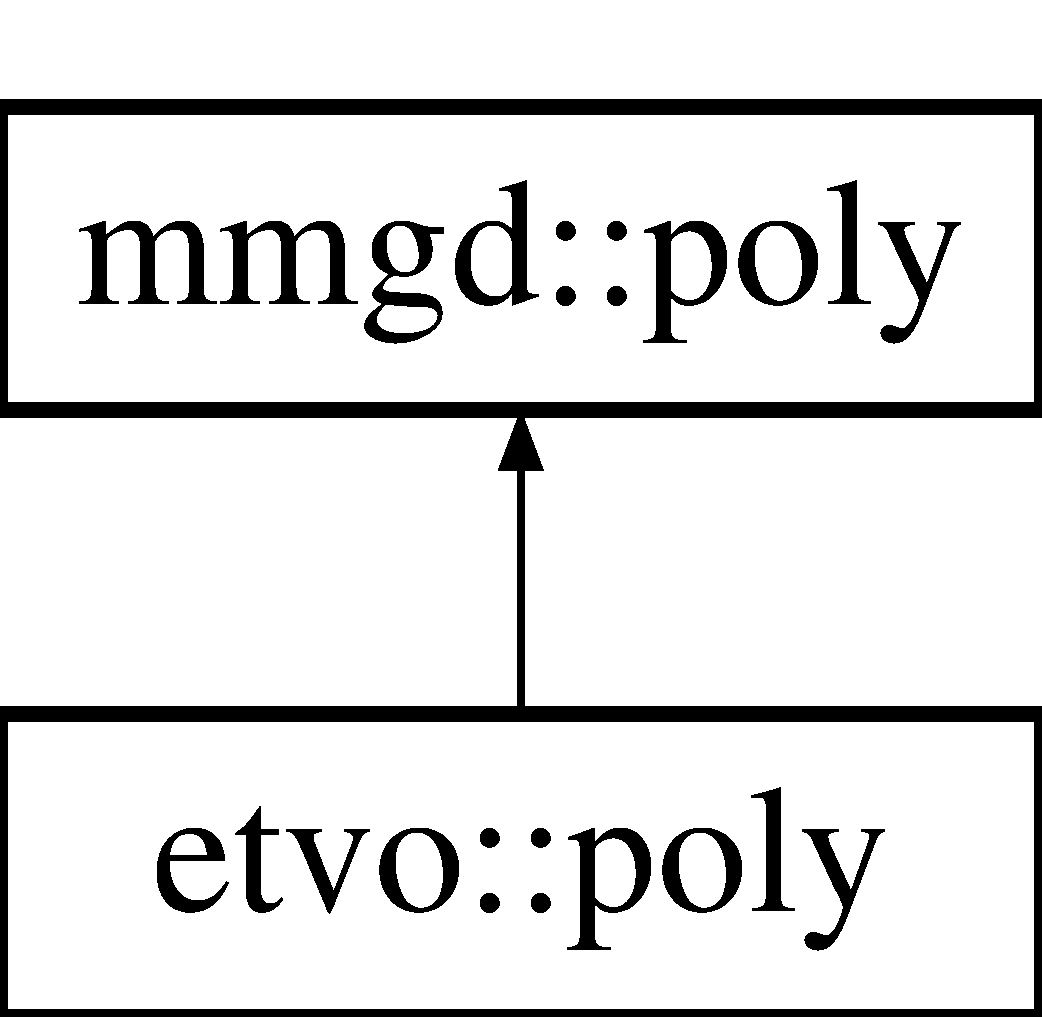
\includegraphics[height=2.000000cm]{classmmgd_1_1poly}
\end{center}
\end{figure}
\subsection*{Public Member Functions}
\begin{DoxyCompactItemize}
\item 
\mbox{\Hypertarget{classmmgd_1_1poly_aeda6ade4af424598ef30767c990a6dea}\label{classmmgd_1_1poly_aeda6ade4af424598ef30767c990a6dea}} 
{\bfseries poly} (const \mbox{\hyperlink{classmmgd_1_1poly}{poly}} \&)
\item 
\mbox{\Hypertarget{classmmgd_1_1poly_ad382086366b79f689dbd7928ecdfdbb5}\label{classmmgd_1_1poly_ad382086366b79f689dbd7928ecdfdbb5}} 
{\bfseries poly} (const \mbox{\hyperlink{classmmgd_1_1gd}{gd}} \&)
\item 
\mbox{\Hypertarget{classmmgd_1_1poly_a133a3b2591c6b3a15a4d4fe03ef3599c}\label{classmmgd_1_1poly_a133a3b2591c6b3a15a4d4fe03ef3599c}} 
{\bfseries poly} (long g, long d)
\item 
\mbox{\Hypertarget{classmmgd_1_1poly_a06487929da588e96a1f63503bad5cd9d}\label{classmmgd_1_1poly_a06487929da588e96a1f63503bad5cd9d}} 
{\bfseries poly} (unsigned int, \mbox{\hyperlink{classmmgd_1_1gd}{gd}} $\ast$)
\item 
\mbox{\Hypertarget{classmmgd_1_1poly_ac9ae9acd1a5d97c73856ff68aaa8f509}\label{classmmgd_1_1poly_ac9ae9acd1a5d97c73856ff68aaa8f509}} 
\mbox{\hyperlink{classmmgd_1_1poly}{poly}} \& {\bfseries operator=} (const \mbox{\hyperlink{classmmgd_1_1poly}{poly}} \&)
\item 
\mbox{\Hypertarget{classmmgd_1_1poly_a593698e5f78e7aa64a143c85c35333f9}\label{classmmgd_1_1poly_a593698e5f78e7aa64a143c85c35333f9}} 
\mbox{\hyperlink{classmmgd_1_1poly}{poly}} \& {\bfseries operator()} (long g, long d)
\item 
\mbox{\Hypertarget{classmmgd_1_1poly_a5d092e747d276a8f38461a0b7d459759}\label{classmmgd_1_1poly_a5d092e747d276a8f38461a0b7d459759}} 
void {\bfseries init} (unsigned int, \mbox{\hyperlink{classmmgd_1_1gd}{gd}} $\ast$, int)
\item 
\mbox{\Hypertarget{classmmgd_1_1poly_aec0dc14f9919d62e2223afb9844d1f08}\label{classmmgd_1_1poly_aec0dc14f9919d62e2223afb9844d1f08}} 
\mbox{\hyperlink{classmmgd_1_1poly}{poly}} \& {\bfseries operator=} (const \mbox{\hyperlink{classmmgd_1_1gd}{gd}} \&gd1)
\item 
\mbox{\Hypertarget{classmmgd_1_1poly_a5bd23732151750b7e29789f6e17b9f6b}\label{classmmgd_1_1poly_a5bd23732151750b7e29789f6e17b9f6b}} 
\mbox{\hyperlink{classmmgd_1_1poly}{poly}} \& {\bfseries init} (long g, long d)
\item 
\mbox{\Hypertarget{classmmgd_1_1poly_ad8b13c9086778f9461ae8460ecca0d28}\label{classmmgd_1_1poly_ad8b13c9086778f9461ae8460ecca0d28}} 
void {\bfseries affecte} (unsigned int, const \mbox{\hyperlink{classmmgd_1_1gd}{gd}} $\ast$, unsigned int propre)
\item 
\mbox{\Hypertarget{classmmgd_1_1poly_ae5b5e62d2e6a5a820b71f939f4d06872}\label{classmmgd_1_1poly_ae5b5e62d2e6a5a820b71f939f4d06872}} 
\mbox{\hyperlink{classmmgd_1_1gd}{gd}} \& {\bfseries getpol} (int i) const
\item 
\mbox{\Hypertarget{classmmgd_1_1poly_a2f4f968f61c7af5aff9e349f65d0da23}\label{classmmgd_1_1poly_a2f4f968f61c7af5aff9e349f65d0da23}} 
unsigned int {\bfseries getn} () const
\item 
\mbox{\Hypertarget{classmmgd_1_1poly_a5495fb6ca0d7c61bb5b206f559ffcf01}\label{classmmgd_1_1poly_a5495fb6ca0d7c61bb5b206f559ffcf01}} 
void {\bfseries setsimple} ()
\item 
\mbox{\Hypertarget{classmmgd_1_1poly_a18c1e001f43ce42745d7b2be6890cc3f}\label{classmmgd_1_1poly_a18c1e001f43ce42745d7b2be6890cc3f}} 
\mbox{\hyperlink{classmmgd_1_1gd}{gd}} $\ast$ {\bfseries getdata} ()
\item 
\mbox{\Hypertarget{classmmgd_1_1poly_a184a9b26eed443676f8d55919856a363}\label{classmmgd_1_1poly_a184a9b26eed443676f8d55919856a363}} 
void {\bfseries popj} (unsigned int j)
\item 
\mbox{\Hypertarget{classmmgd_1_1poly_a8b72b2a38fe605ee83d03c546315feaa}\label{classmmgd_1_1poly_a8b72b2a38fe605ee83d03c546315feaa}} 
void {\bfseries pop} ()
\item 
\mbox{\Hypertarget{classmmgd_1_1poly_a0b40ee1475cd9d321ddea43dde871321}\label{classmmgd_1_1poly_a0b40ee1475cd9d321ddea43dde871321}} 
void {\bfseries add} (const \mbox{\hyperlink{classmmgd_1_1gd}{gd}} \&m1)
\item 
\mbox{\Hypertarget{classmmgd_1_1poly_a49ff0c355621ee90b83986b5c21a681b}\label{classmmgd_1_1poly_a49ff0c355621ee90b83986b5c21a681b}} 
void {\bfseries simpli} ()
\item 
\mbox{\Hypertarget{classmmgd_1_1poly_a7c0e2e60fb473ecd70af742d6cfb8214}\label{classmmgd_1_1poly_a7c0e2e60fb473ecd70af742d6cfb8214}} 
void {\bfseries onlysimpli} ()
\item 
\mbox{\Hypertarget{classmmgd_1_1poly_a5033ce10a8708ca2a6d43d31ac0abb70}\label{classmmgd_1_1poly_a5033ce10a8708ca2a6d43d31ac0abb70}} 
void {\bfseries swapgd} (\mbox{\hyperlink{classmmgd_1_1gd}{gd}} \&a, \mbox{\hyperlink{classmmgd_1_1gd}{gd}} \&b)
\item 
\mbox{\Hypertarget{classmmgd_1_1poly_ab3bd363ed00bc3be3d31b0e9e79debde}\label{classmmgd_1_1poly_ab3bd363ed00bc3be3d31b0e9e79debde}} 
int {\bfseries partitionner} (\mbox{\hyperlink{classmmgd_1_1gd}{gd}} $\ast$tab, int debut, int dernier, int pivot, int comp(const void $\ast$, const void $\ast$))
\item 
\mbox{\Hypertarget{classmmgd_1_1poly_ae121ae3e10e8252bc9b9c1b745867a8b}\label{classmmgd_1_1poly_ae121ae3e10e8252bc9b9c1b745867a8b}} 
int {\bfseries operator==} (const \mbox{\hyperlink{classmmgd_1_1poly}{poly}} \&)
\end{DoxyCompactItemize}
\subsection*{Static Public Attributes}
\begin{DoxyCompactItemize}
\item 
\mbox{\Hypertarget{classmmgd_1_1poly_a4c658d3ff941048a220fe08f3bc2dfab}\label{classmmgd_1_1poly_a4c658d3ff941048a220fe08f3bc2dfab}} 
static int {\bfseries forcage} =0
\end{DoxyCompactItemize}
\subsection*{Friends}
\begin{DoxyCompactItemize}
\item 
\mbox{\Hypertarget{classmmgd_1_1poly_a902bbbf11a23a3fc4075dcd29e9ba0a3}\label{classmmgd_1_1poly_a902bbbf11a23a3fc4075dcd29e9ba0a3}} 
int {\bfseries compgd} (const void $\ast$p1, const void $\ast$p2)
\item 
\mbox{\Hypertarget{classmmgd_1_1poly_a6e11338fa76cb7916e75802534f77587}\label{classmmgd_1_1poly_a6e11338fa76cb7916e75802534f77587}} 
void {\bfseries qsort\+\_\+gd} (\mbox{\hyperlink{classmmgd_1_1gd}{gd}} $\ast$adtab, int premier, int dernier, int comp(const void $\ast$, const void $\ast$))
\item 
\mbox{\Hypertarget{classmmgd_1_1poly_abcce92100cdf3208f275859d3908fbe6}\label{classmmgd_1_1poly_abcce92100cdf3208f275859d3908fbe6}} 
\mbox{\hyperlink{classmmgd_1_1poly}{poly}} {\bfseries oplus} (\mbox{\hyperlink{classmmgd_1_1poly}{poly}} \&, \mbox{\hyperlink{classmmgd_1_1poly}{poly}} \&)
\item 
\mbox{\Hypertarget{classmmgd_1_1poly_a247e64e536c6f1a070bc8eb9d870058d}\label{classmmgd_1_1poly_a247e64e536c6f1a070bc8eb9d870058d}} 
\mbox{\hyperlink{classmmgd_1_1poly}{poly}} {\bfseries oplus} (\mbox{\hyperlink{classmmgd_1_1gd}{gd}} \&, \mbox{\hyperlink{classmmgd_1_1gd}{gd}} \&)
\item 
\mbox{\Hypertarget{classmmgd_1_1poly_a8408c8cbe50239231608be92b6c8b47f}\label{classmmgd_1_1poly_a8408c8cbe50239231608be92b6c8b47f}} 
\mbox{\hyperlink{classmmgd_1_1poly}{poly}} {\bfseries oplus} (\mbox{\hyperlink{classmmgd_1_1poly}{poly}} \&, \mbox{\hyperlink{classmmgd_1_1gd}{gd}} \&)
\item 
\mbox{\Hypertarget{classmmgd_1_1poly_a7d137100cfb94e8231c00c253b1c0d45}\label{classmmgd_1_1poly_a7d137100cfb94e8231c00c253b1c0d45}} 
\mbox{\hyperlink{classmmgd_1_1poly}{poly}} {\bfseries oplus} (\mbox{\hyperlink{classmmgd_1_1gd}{gd}} \&, \mbox{\hyperlink{classmmgd_1_1poly}{poly}} \&)
\item 
\mbox{\Hypertarget{classmmgd_1_1poly_aa457431adea4b51f375222c772dfa926}\label{classmmgd_1_1poly_aa457431adea4b51f375222c772dfa926}} 
\mbox{\hyperlink{classmmgd_1_1poly}{poly}} {\bfseries oplus} (\mbox{\hyperlink{classmmgd_1_1poly}{poly}} \&, \mbox{\hyperlink{classmmgd_1_1poly}{poly}} \&, \mbox{\hyperlink{classmmgd_1_1poly}{poly}} \&)
\item 
\mbox{\Hypertarget{classmmgd_1_1poly_a035bd6940202bdaefbd9f15b65aca4c7}\label{classmmgd_1_1poly_a035bd6940202bdaefbd9f15b65aca4c7}} 
\mbox{\hyperlink{classmmgd_1_1poly}{poly}} {\bfseries oplus} (\mbox{\hyperlink{classmmgd_1_1poly}{poly}} \&, \mbox{\hyperlink{classmmgd_1_1poly}{poly}} \&, \mbox{\hyperlink{classmmgd_1_1poly}{poly}} \&, \mbox{\hyperlink{classmmgd_1_1poly}{poly}} \&)
\item 
\mbox{\Hypertarget{classmmgd_1_1poly_adc4c4b3ff5bde03992056d6293de8adc}\label{classmmgd_1_1poly_adc4c4b3ff5bde03992056d6293de8adc}} 
\mbox{\hyperlink{classmmgd_1_1poly}{poly}} {\bfseries otimes} (\mbox{\hyperlink{classmmgd_1_1poly}{poly}} \&poly1, \mbox{\hyperlink{classmmgd_1_1poly}{poly}} \&poly2)
\item 
\mbox{\Hypertarget{classmmgd_1_1poly_ab6880d5f38b5617b51b536cc12dbe632}\label{classmmgd_1_1poly_ab6880d5f38b5617b51b536cc12dbe632}} 
\mbox{\hyperlink{classmmgd_1_1poly}{poly}} {\bfseries otimes} (\mbox{\hyperlink{classmmgd_1_1poly}{poly}} \&poly1, \mbox{\hyperlink{classmmgd_1_1gd}{gd}} \&gd2)
\item 
\mbox{\Hypertarget{classmmgd_1_1poly_a48427a3900629c5a386cbc2817f16e55}\label{classmmgd_1_1poly_a48427a3900629c5a386cbc2817f16e55}} 
\mbox{\hyperlink{classmmgd_1_1poly}{poly}} {\bfseries otimes} (\mbox{\hyperlink{classmmgd_1_1gd}{gd}} \&gd1, \mbox{\hyperlink{classmmgd_1_1poly}{poly}} \&poly2)
\item 
\mbox{\Hypertarget{classmmgd_1_1poly_a803937f55e9be138336bd21748fea019}\label{classmmgd_1_1poly_a803937f55e9be138336bd21748fea019}} 
\mbox{\hyperlink{classmmgd_1_1poly}{poly}} {\bfseries inf} (\mbox{\hyperlink{classmmgd_1_1poly}{poly}} \&poly1, \mbox{\hyperlink{classmmgd_1_1poly}{poly}} \&poly2)
\item 
\mbox{\Hypertarget{classmmgd_1_1poly_a03fcc1a1d0999a26f741958726ad8786}\label{classmmgd_1_1poly_a03fcc1a1d0999a26f741958726ad8786}} 
\mbox{\hyperlink{classmmgd_1_1poly}{poly}} {\bfseries inf} (\mbox{\hyperlink{classmmgd_1_1poly}{poly}} \&poly1, \mbox{\hyperlink{classmmgd_1_1gd}{gd}} \&gd2)
\item 
\mbox{\Hypertarget{classmmgd_1_1poly_a201336586d8f06607e606a71d56d0620}\label{classmmgd_1_1poly_a201336586d8f06607e606a71d56d0620}} 
\mbox{\hyperlink{classmmgd_1_1poly}{poly}} {\bfseries inf} (\mbox{\hyperlink{classmmgd_1_1gd}{gd}} \&gd1, \mbox{\hyperlink{classmmgd_1_1poly}{poly}} \&poly2)
\item 
\mbox{\Hypertarget{classmmgd_1_1poly_a1ca2365b15ec5d9647e2ee8cc82bc0c3}\label{classmmgd_1_1poly_a1ca2365b15ec5d9647e2ee8cc82bc0c3}} 
\mbox{\hyperlink{classmmgd_1_1poly}{poly}} {\bfseries frac} (\mbox{\hyperlink{classmmgd_1_1poly}{poly}} \&poly1, \mbox{\hyperlink{classmmgd_1_1gd}{gd}} \&gd2)
\item 
\mbox{\Hypertarget{classmmgd_1_1poly_a2bb496ce83846bee4b6273821e059827}\label{classmmgd_1_1poly_a2bb496ce83846bee4b6273821e059827}} 
\mbox{\hyperlink{classmmgd_1_1poly}{poly}} {\bfseries frac} (\mbox{\hyperlink{classmmgd_1_1poly}{poly}} \&poly1, \mbox{\hyperlink{classmmgd_1_1poly}{poly}} \&poly2)
\item 
\mbox{\Hypertarget{classmmgd_1_1poly_af8dd7f52f6fa54f4f40d657652b14a54}\label{classmmgd_1_1poly_af8dd7f52f6fa54f4f40d657652b14a54}} 
\mbox{\hyperlink{classmmgd_1_1poly}{poly}} {\bfseries frac} (\mbox{\hyperlink{classmmgd_1_1gd}{gd}} \&gd1, \mbox{\hyperlink{classmmgd_1_1poly}{poly}} \&poly2)
\item 
\mbox{\Hypertarget{classmmgd_1_1poly_ad9580516418e4c9c5ee22b7f67cfb6ee}\label{classmmgd_1_1poly_ad9580516418e4c9c5ee22b7f67cfb6ee}} 
\mbox{\hyperlink{classmmgd_1_1poly}{poly}} {\bfseries prcaus} (\mbox{\hyperlink{classmmgd_1_1poly}{poly}} \&)
\item 
\mbox{\Hypertarget{classmmgd_1_1poly_a0361c355a8ea5d7e13ec20144390082f}\label{classmmgd_1_1poly_a0361c355a8ea5d7e13ec20144390082f}} 
std\+::ostream \& {\bfseries operator$<$$<$} (std\+::ostream \&, \mbox{\hyperlink{classmmgd_1_1poly}{poly}} \&)
\item 
\mbox{\Hypertarget{classmmgd_1_1poly_af0ab9a74b034ed507c6070d9a47951b8}\label{classmmgd_1_1poly_af0ab9a74b034ed507c6070d9a47951b8}} 
std\+::fstream \& {\bfseries operator$<$$<$} (std\+::fstream \&, \mbox{\hyperlink{classmmgd_1_1poly}{poly}} \&)
\item 
\mbox{\Hypertarget{classmmgd_1_1poly_a9cecbf55fe370b38e24b8b639fd1ee03}\label{classmmgd_1_1poly_a9cecbf55fe370b38e24b8b639fd1ee03}} 
\mbox{\hyperlink{classmmgd_1_1poly}{poly}} {\bfseries odot} (const \mbox{\hyperlink{classmmgd_1_1poly}{poly}} \&poly1, const \mbox{\hyperlink{classmmgd_1_1poly}{poly}} \&poly2)
\item 
\mbox{\Hypertarget{classmmgd_1_1poly_aff323f3e36b51b89ff4b52ffdf7464dd}\label{classmmgd_1_1poly_aff323f3e36b51b89ff4b52ffdf7464dd}} 
\mbox{\hyperlink{classmmgd_1_1poly}{poly}} {\bfseries fracodotsharp} (\mbox{\hyperlink{classmmgd_1_1poly}{poly}} \&poly1, \mbox{\hyperlink{classmmgd_1_1poly}{poly}} \&poly2)
\item 
\mbox{\Hypertarget{classmmgd_1_1poly_ad284d1dbb550ed9c6a6ad3f9f3e2e3cc}\label{classmmgd_1_1poly_ad284d1dbb550ed9c6a6ad3f9f3e2e3cc}} 
\mbox{\hyperlink{classmmgd_1_1poly}{poly}} {\bfseries fracodotflat} (\mbox{\hyperlink{classmmgd_1_1poly}{poly}} \&poly1, \mbox{\hyperlink{classmmgd_1_1poly}{poly}} \&poly2)
\end{DoxyCompactItemize}


The documentation for this class was generated from the following files\+:\begin{DoxyCompactItemize}
\item 
etvo/minmaxgd/poly.\+h\item 
etvo/minmaxgd/poly.\+cpp\end{DoxyCompactItemize}

\section{mmgd\+:\+:mmgd\+:\+:poly Class Reference}
\label{classmmgd_1_1mmgd_1_1poly}\index{mmgd\+::mmgd\+::poly@{mmgd\+::mmgd\+::poly}}
\subsection*{Public Member Functions}
\begin{DoxyCompactItemize}
\item 
\mbox{\label{classmmgd_1_1mmgd_1_1poly_aeda6ade4af424598ef30767c990a6dea}} 
{\bfseries poly} (const \textbf{ poly} \&)
\item 
\mbox{\label{classmmgd_1_1mmgd_1_1poly_ad382086366b79f689dbd7928ecdfdbb5}} 
{\bfseries poly} (const \textbf{ gd} \&)
\item 
\mbox{\label{classmmgd_1_1mmgd_1_1poly_a133a3b2591c6b3a15a4d4fe03ef3599c}} 
{\bfseries poly} (long g, long d)
\item 
\mbox{\label{classmmgd_1_1mmgd_1_1poly_a06487929da588e96a1f63503bad5cd9d}} 
{\bfseries poly} (unsigned int, \textbf{ gd} $\ast$)
\item 
\mbox{\label{classmmgd_1_1mmgd_1_1poly_ac9ae9acd1a5d97c73856ff68aaa8f509}} 
\textbf{ poly} \& {\bfseries operator=} (const \textbf{ poly} \&)
\item 
\mbox{\label{classmmgd_1_1mmgd_1_1poly_a593698e5f78e7aa64a143c85c35333f9}} 
\textbf{ poly} \& {\bfseries operator()} (long g, long d)
\item 
\mbox{\label{classmmgd_1_1mmgd_1_1poly_a5d092e747d276a8f38461a0b7d459759}} 
void {\bfseries init} (unsigned int, \textbf{ gd} $\ast$, int)
\item 
\mbox{\label{classmmgd_1_1mmgd_1_1poly_aec0dc14f9919d62e2223afb9844d1f08}} 
\textbf{ poly} \& {\bfseries operator=} (const \textbf{ gd} \&gd1)
\item 
\mbox{\label{classmmgd_1_1mmgd_1_1poly_a5bd23732151750b7e29789f6e17b9f6b}} 
\textbf{ poly} \& {\bfseries init} (long g, long d)
\item 
\mbox{\label{classmmgd_1_1mmgd_1_1poly_ad8b13c9086778f9461ae8460ecca0d28}} 
void {\bfseries affecte} (unsigned int, const \textbf{ gd} $\ast$, unsigned int propre)
\item 
\mbox{\label{classmmgd_1_1mmgd_1_1poly_ae0b3634dd97dd3512b71b10efcbe28b5}} 
\textbf{ gd} \& {\bfseries getpol} (int i) const
\item 
\mbox{\label{classmmgd_1_1mmgd_1_1poly_a426ca1d32672f822a8ab4fad4fa686f1}} 
unsigned int {\bfseries getn} () const
\item 
\mbox{\label{classmmgd_1_1mmgd_1_1poly_aa746644a922405f6903d54657d4a23d8}} 
void {\bfseries setsimple} ()
\item 
\mbox{\label{classmmgd_1_1mmgd_1_1poly_a7d94298c4fb9eaca0c40f9aa87411084}} 
\textbf{ gd} $\ast$ {\bfseries getdata} ()
\item 
\mbox{\label{classmmgd_1_1mmgd_1_1poly_a184a9b26eed443676f8d55919856a363}} 
void {\bfseries popj} (unsigned int j)
\item 
\mbox{\label{classmmgd_1_1mmgd_1_1poly_a8b72b2a38fe605ee83d03c546315feaa}} 
void {\bfseries pop} ()
\item 
\mbox{\label{classmmgd_1_1mmgd_1_1poly_a0b40ee1475cd9d321ddea43dde871321}} 
void {\bfseries add} (const \textbf{ gd} \&m1)
\item 
\mbox{\label{classmmgd_1_1mmgd_1_1poly_a49ff0c355621ee90b83986b5c21a681b}} 
void {\bfseries simpli} ()
\item 
\mbox{\label{classmmgd_1_1mmgd_1_1poly_a7c0e2e60fb473ecd70af742d6cfb8214}} 
void {\bfseries onlysimpli} ()
\item 
\mbox{\label{classmmgd_1_1mmgd_1_1poly_ad68f2edd232976c15cd58ce821376c28}} 
void {\bfseries swapgd} (\textbf{ gd} \&a, \textbf{ gd} \&b)
\item 
\mbox{\label{classmmgd_1_1mmgd_1_1poly_a1ab826d07bbcdab487006a492c21a2fb}} 
int {\bfseries partitionner} (\textbf{ gd} $\ast$tab, int debut, int dernier, int pivot, int comp(const void $\ast$, const void $\ast$))
\item 
\mbox{\label{classmmgd_1_1mmgd_1_1poly_ae121ae3e10e8252bc9b9c1b745867a8b}} 
int {\bfseries operator==} (const \textbf{ poly} \&)
\end{DoxyCompactItemize}
\subsection*{Friends}
\begin{DoxyCompactItemize}
\item 
\mbox{\label{classmmgd_1_1mmgd_1_1poly_a902bbbf11a23a3fc4075dcd29e9ba0a3}} 
int {\bfseries compgd} (const void $\ast$p1, const void $\ast$p2)
\item 
\mbox{\label{classmmgd_1_1mmgd_1_1poly_a6e11338fa76cb7916e75802534f77587}} 
void {\bfseries qsort\+\_\+gd} (\textbf{ gd} $\ast$adtab, int premier, int dernier, int comp(const void $\ast$, const void $\ast$))
\item 
\mbox{\label{classmmgd_1_1mmgd_1_1poly_abcce92100cdf3208f275859d3908fbe6}} 
\textbf{ poly} {\bfseries oplus} (\textbf{ poly} \&, \textbf{ poly} \&)
\item 
\mbox{\label{classmmgd_1_1mmgd_1_1poly_a247e64e536c6f1a070bc8eb9d870058d}} 
\textbf{ poly} {\bfseries oplus} (\textbf{ gd} \&, \textbf{ gd} \&)
\item 
\mbox{\label{classmmgd_1_1mmgd_1_1poly_a8408c8cbe50239231608be92b6c8b47f}} 
\textbf{ poly} {\bfseries oplus} (\textbf{ poly} \&, \textbf{ gd} \&)
\item 
\mbox{\label{classmmgd_1_1mmgd_1_1poly_a7d137100cfb94e8231c00c253b1c0d45}} 
\textbf{ poly} {\bfseries oplus} (\textbf{ gd} \&, \textbf{ poly} \&)
\item 
\mbox{\label{classmmgd_1_1mmgd_1_1poly_aa457431adea4b51f375222c772dfa926}} 
\textbf{ poly} {\bfseries oplus} (\textbf{ poly} \&, \textbf{ poly} \&, \textbf{ poly} \&)
\item 
\mbox{\label{classmmgd_1_1mmgd_1_1poly_a035bd6940202bdaefbd9f15b65aca4c7}} 
\textbf{ poly} {\bfseries oplus} (\textbf{ poly} \&, \textbf{ poly} \&, \textbf{ poly} \&, \textbf{ poly} \&)
\item 
\mbox{\label{classmmgd_1_1mmgd_1_1poly_adc4c4b3ff5bde03992056d6293de8adc}} 
\textbf{ poly} {\bfseries otimes} (\textbf{ poly} \&poly1, \textbf{ poly} \&poly2)
\item 
\mbox{\label{classmmgd_1_1mmgd_1_1poly_ab6880d5f38b5617b51b536cc12dbe632}} 
\textbf{ poly} {\bfseries otimes} (\textbf{ poly} \&poly1, \textbf{ gd} \&gd2)
\item 
\mbox{\label{classmmgd_1_1mmgd_1_1poly_a48427a3900629c5a386cbc2817f16e55}} 
\textbf{ poly} {\bfseries otimes} (\textbf{ gd} \&gd1, \textbf{ poly} \&poly2)
\item 
\mbox{\label{classmmgd_1_1mmgd_1_1poly_a803937f55e9be138336bd21748fea019}} 
\textbf{ poly} {\bfseries inf} (\textbf{ poly} \&poly1, \textbf{ poly} \&poly2)
\item 
\mbox{\label{classmmgd_1_1mmgd_1_1poly_a03fcc1a1d0999a26f741958726ad8786}} 
\textbf{ poly} {\bfseries inf} (\textbf{ poly} \&poly1, \textbf{ gd} \&gd2)
\item 
\mbox{\label{classmmgd_1_1mmgd_1_1poly_a201336586d8f06607e606a71d56d0620}} 
\textbf{ poly} {\bfseries inf} (\textbf{ gd} \&gd1, \textbf{ poly} \&poly2)
\item 
\mbox{\label{classmmgd_1_1mmgd_1_1poly_a1ca2365b15ec5d9647e2ee8cc82bc0c3}} 
\textbf{ poly} {\bfseries frac} (\textbf{ poly} \&poly1, \textbf{ gd} \&gd2)
\item 
\mbox{\label{classmmgd_1_1mmgd_1_1poly_a2bb496ce83846bee4b6273821e059827}} 
\textbf{ poly} {\bfseries frac} (\textbf{ poly} \&poly1, \textbf{ poly} \&poly2)
\item 
\mbox{\label{classmmgd_1_1mmgd_1_1poly_af8dd7f52f6fa54f4f40d657652b14a54}} 
\textbf{ poly} {\bfseries frac} (\textbf{ gd} \&gd1, \textbf{ poly} \&poly2)
\item 
\mbox{\label{classmmgd_1_1mmgd_1_1poly_ad9580516418e4c9c5ee22b7f67cfb6ee}} 
\textbf{ poly} {\bfseries prcaus} (\textbf{ poly} \&)
\item 
\mbox{\label{classmmgd_1_1mmgd_1_1poly_a0361c355a8ea5d7e13ec20144390082f}} 
std\+::ostream \& {\bfseries operator$<$$<$} (std\+::ostream \&, \textbf{ poly} \&)
\item 
\mbox{\label{classmmgd_1_1mmgd_1_1poly_af0ab9a74b034ed507c6070d9a47951b8}} 
std\+::fstream \& {\bfseries operator$<$$<$} (std\+::fstream \&, \textbf{ poly} \&)
\item 
\mbox{\label{classmmgd_1_1mmgd_1_1poly_a9cecbf55fe370b38e24b8b639fd1ee03}} 
\textbf{ poly} {\bfseries odot} (const \textbf{ poly} \&poly1, const \textbf{ poly} \&poly2)
\item 
\mbox{\label{classmmgd_1_1mmgd_1_1poly_aff323f3e36b51b89ff4b52ffdf7464dd}} 
\textbf{ poly} {\bfseries fracodotsharp} (\textbf{ poly} \&poly1, \textbf{ poly} \&poly2)
\item 
\mbox{\label{classmmgd_1_1mmgd_1_1poly_ad284d1dbb550ed9c6a6ad3f9f3e2e3cc}} 
\textbf{ poly} {\bfseries fracodotflat} (\textbf{ poly} \&poly1, \textbf{ poly} \&poly2)
\end{DoxyCompactItemize}


The documentation for this class was generated from the following file\+:\begin{DoxyCompactItemize}
\item 
F\+:/\+U\+A Box/\+Dev\+Soft/etvo\+I\+I\+I/etvo21/etvo/libminmaxgd/src/poly.\+cpp\end{DoxyCompactItemize}

\section{etvo\+:\+:poly\+Ed Class Reference}
\label{classetvo_1_1poly_ed}\index{etvo\+::poly\+Ed@{etvo\+::poly\+Ed}}


Class for polynomials in the semiring E[[d]].  




{\ttfamily \#include $<$poly\+Ed.\+h$>$}

Inheritance diagram for etvo\+:\+:poly\+Ed\+:\begin{figure}[H]
\begin{center}
\leavevmode
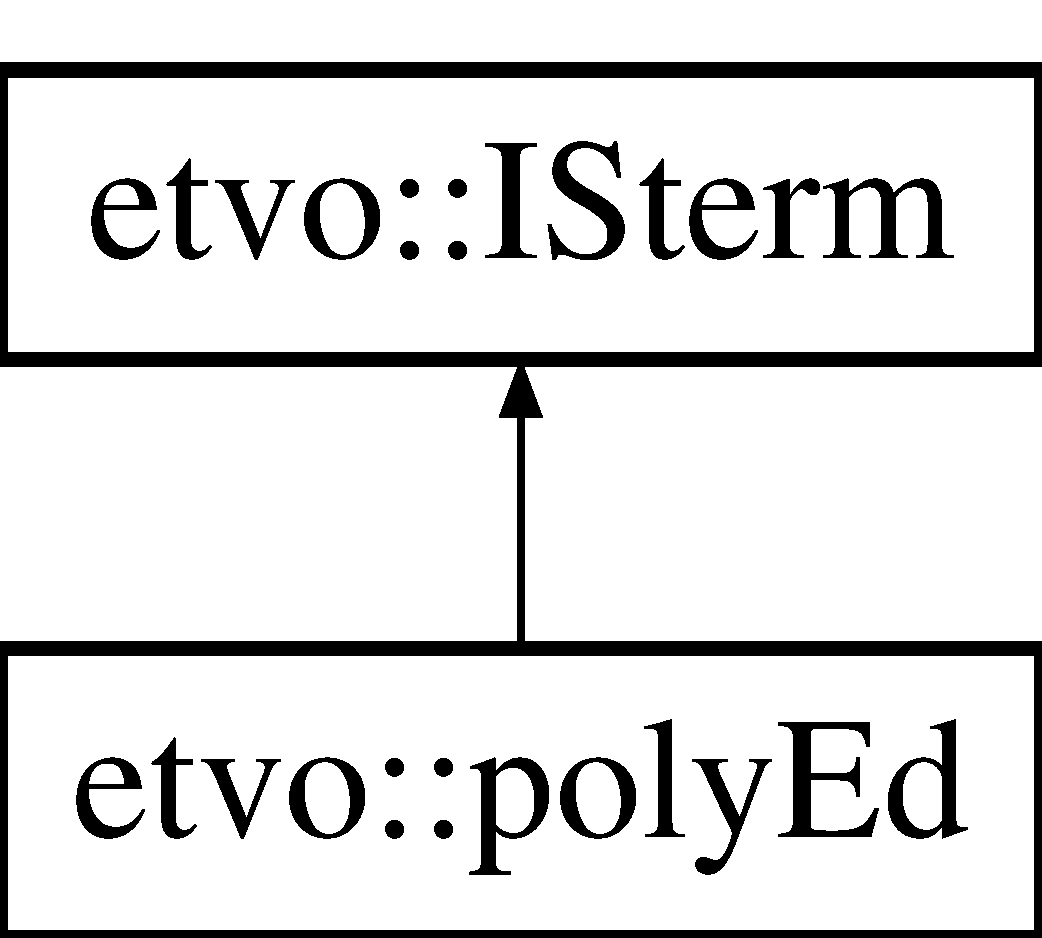
\includegraphics[height=2.000000cm]{classetvo_1_1poly_ed}
\end{center}
\end{figure}
\subsection*{Public Member Functions}
\begin{DoxyCompactItemize}
\item 
\mbox{\label{classetvo_1_1poly_ed_a82aa32fb16af0436d94beb915e50d158}} 
\textbf{ poly\+Ed} ()
\begin{DoxyCompactList}\small\item\em default initialization to Epsilon \end{DoxyCompactList}\item 
\mbox{\label{classetvo_1_1poly_ed_ab5c5bc5383986ba9d48373fe277c38c5}} 
\textbf{ poly\+Ed} (bool Top\+NotE)
\begin{DoxyCompactList}\small\item\em specific initialization \+: poly\+Ed(true) set to Top, poly\+Ed(false) set to E \end{DoxyCompactList}\item 
\mbox{\label{classetvo_1_1poly_ed_a3b2bdd141d15d15c90474dd3dd6766f0}} 
\textbf{ poly\+Ed} (const \textbf{ Ed} \&m)
\begin{DoxyCompactList}\small\item\em initialisation to a polynomial with one \doxyref{Ed}{p.}{classetvo_1_1_ed} term w.\+d$^\wedge$t \end{DoxyCompactList}\item 
\textbf{ poly\+Ed} (const std\+::vector$<$ \textbf{ Ed} $>$ \&v)
\item 
\mbox{\label{classetvo_1_1poly_ed_a9010ec718c914d0b004a9a6a77014094}} 
\textbf{ poly} \textbf{ to\+Poly} () const
\begin{DoxyCompactList}\small\item\em The zero-\/slice polynomial in Min\+Max[[g,d]]. \end{DoxyCompactList}\item 
\mbox{\label{classetvo_1_1poly_ed_ac83a3de206764082e6b2b640e416e771}} 
\textbf{ poly\+Ed} \textbf{ operator+} (const \textbf{ poly\+Ed} \&p) const
\begin{DoxyCompactList}\small\item\em Sum of polynomials in E[[d]]. \end{DoxyCompactList}\item 
\mbox{\label{classetvo_1_1poly_ed_ac87c88989209880ec06bd7b147e915ab}} 
\textbf{ poly\+Ed} \textbf{ oplus} (const \textbf{ poly\+Ed} \&p) const
\begin{DoxyCompactList}\small\item\em Sum of polynomials in E[[d]]. \end{DoxyCompactList}\item 
\mbox{\label{classetvo_1_1poly_ed_ac634c723e5f8d624776000163d4926d7}} 
\textbf{ poly\+Ed} \textbf{ oplus\+CD} (const \textbf{ poly\+Ed} \&p) const
\begin{DoxyCompactList}\small\item\em Sum of polynomials in E[[d]] via a Core Decomposition (see J.\+Trunk Thesis) \end{DoxyCompactList}\item 
\mbox{\label{classetvo_1_1poly_ed_ae869c9df48cd94a04c06b5b687322e74}} 
\textbf{ poly\+Ed} \textbf{ operator+} (const \textbf{ Ed} \&m) const
\begin{DoxyCompactList}\small\item\em Sum of a polynomial in E[[d]] with a monomial in E[[d]]. \end{DoxyCompactList}\item 
\mbox{\label{classetvo_1_1poly_ed_afb88ad949598bd94f720f6e7e453e91e}} 
void \textbf{ add} (const \textbf{ Ed} \&m)
\begin{DoxyCompactList}\small\item\em The current polynomial pcur is modified as pcur=pcur+m. \end{DoxyCompactList}\item 
\mbox{\label{classetvo_1_1poly_ed_a4d524f339d16a17c4a1abc5ff6837a47}} 
\textbf{ poly\+Ed} \textbf{ operator+=} (const \textbf{ Ed} \&m)
\begin{DoxyCompactList}\small\item\em Lies on \doxyref{poly\+Ed\+::add(const Ed \& m)}{p.}{classetvo_1_1poly_ed_afb88ad949598bd94f720f6e7e453e91e} method. \end{DoxyCompactList}\item 
\mbox{\label{classetvo_1_1poly_ed_a69a3d0b6df800f2d735ec550c6325ef5}} 
\textbf{ poly\+Ed} \textbf{ operator$\ast$} (const \textbf{ poly\+Ed} \&p) const
\begin{DoxyCompactList}\small\item\em Product of polynomials in E[[d]]. \end{DoxyCompactList}\item 
\mbox{\label{classetvo_1_1poly_ed_a3785ebbd0f0b9e1ac4007f1ea6ce9cb4}} 
\textbf{ poly\+Ed} \textbf{ operator$\ast$} (const \textbf{ Ed} \&m) const
\begin{DoxyCompactList}\small\item\em Product of one polynomial by one monomial in E[[d]]. \end{DoxyCompactList}\item 
\mbox{\label{classetvo_1_1poly_ed_abf6db66a71df90aec21b5c81e57321dc}} 
\textbf{ poly\+Ed} \textbf{ otimes} (const \textbf{ poly\+Ed} \&p) const
\begin{DoxyCompactList}\small\item\em Product of polynomials in E[[d]]. \end{DoxyCompactList}\item 
\mbox{\label{classetvo_1_1poly_ed_a8fa9e4ea0540cf0db6348661efb407ed}} 
\textbf{ poly\+Ed} \textbf{ otimes\+CD} (const \textbf{ poly\+Ed} \&p) const
\begin{DoxyCompactList}\small\item\em Product of polynomials in E[[d]] via a Core Decomposition (see j.\+Trunk thesis) \end{DoxyCompactList}\item 
\mbox{\label{classetvo_1_1poly_ed_a34ea58c110bbdce153195ca73afbfc8f}} 
\textbf{ poly\+Ed} \textbf{ inf} (const \textbf{ poly\+Ed} \&p) const
\begin{DoxyCompactList}\small\item\em Infimum of two polynomials in E[[d]] \+: p1.\+inf(p2) = greatest x s.\+t. x$<$=p1 and x$<$=p2. \end{DoxyCompactList}\item 
\textbf{ poly\+Ed} \textbf{ inf\+CD} (const \textbf{ poly\+Ed} \&p) const
\item 
\textbf{ series\+Ed} \textbf{ star} () const
\item 
\mbox{\label{classetvo_1_1poly_ed_a48b58fe08414b910b2ed6361e050aeee}} 
\textbf{ poly\+Ed} \textbf{ lfrac} (const \textbf{ poly\+Ed} \&) const
\begin{DoxyCompactList}\small\item\em Computation of the left-\/multiplication residuation\+: p1.\+lfrac(p2) =p2= greatest x s.\+t. p2.\+x $<$= p1. \end{DoxyCompactList}\item 
\textbf{ poly\+Ed} \textbf{ lfrac\+CD} (const \textbf{ poly\+Ed} \&) const
\item 
\mbox{\label{classetvo_1_1poly_ed_a4d5795908c3633c453bca87b71a6dfbb}} 
\textbf{ poly\+Ed} \textbf{ lfrac} (const \textbf{ Ed} \&m) const
\begin{DoxyCompactList}\small\item\em Computation of the left-\/multiplication residuation\+: p1.\+lfrac(m) =m= greatest x s.\+t. m.\+x $<$= p1. \end{DoxyCompactList}\item 
\mbox{\label{classetvo_1_1poly_ed_a922eac49bf439b0f09191ce39a78e492}} 
\textbf{ poly\+Ed} \textbf{ rfrac} (const \textbf{ poly\+Ed} \&) const
\begin{DoxyCompactList}\small\item\em Computation of the right-\/multiplication residuation\+: p1.\+rfrac(p2) =p1/p2= greatest x s.\+t. x.\+p2 $<$= p1. \end{DoxyCompactList}\item 
\textbf{ poly\+Ed} \textbf{ rfrac\+CD} (const \textbf{ poly\+Ed} \&) const
\item 
\mbox{\label{classetvo_1_1poly_ed_aa8512adb43e328f910904195295d94a4}} 
\textbf{ poly\+Ed} \textbf{ rfrac} (const \textbf{ Ed} \&m) const
\begin{DoxyCompactList}\small\item\em Computation of the right-\/multiplication residuation\+: p1.\+rfrac(m) =p1/m= greatest x s.\+t. x.\+m $<$= p1. \end{DoxyCompactList}\item 
\mbox{\label{classetvo_1_1poly_ed_ae4e2a5688b9c49b3ac2e98f8c55fa76c}} 
bool \textbf{ operator==} (const \textbf{ poly\+Ed} \&) const
\begin{DoxyCompactList}\small\item\em Check equality. \end{DoxyCompactList}\item 
\mbox{\label{classetvo_1_1poly_ed_af9466b6fddac07d961a5ddb348ff8ca6}} 
bool \textbf{ operator!=} (const \textbf{ poly\+Ed} \&) const
\begin{DoxyCompactList}\small\item\em Check difference. \end{DoxyCompactList}\item 
\mbox{\label{classetvo_1_1poly_ed_a6913357b93e582d5215e49a97659dc81}} 
bool \textbf{ operator$<$=} (const \textbf{ poly\+Ed} \&) const
\begin{DoxyCompactList}\small\item\em Check order on polynomials in E[[d]]. \end{DoxyCompactList}\item 
\mbox{\label{classetvo_1_1poly_ed_ad54a41a94587da3ccb475b3ccd484831}} 
bool \textbf{ operator$>$=} (const \textbf{ poly\+Ed} \&) const
\begin{DoxyCompactList}\small\item\em Check order on polynomials in E[[d]]. \end{DoxyCompactList}\item 
\textbf{ Ed} \textbf{ get\+First\+Dif} (const \textbf{ poly\+Ed} \&p) const
\item 
\mbox{\label{classetvo_1_1poly_ed_a6fd62867c15fa17a16ac1ed4963f69be}} 
\textbf{ poly\+Ed} \textbf{ transient\+Star} (int Tmax) const
\begin{DoxyCompactList}\small\item\em Do not use it. Use \doxyref{poly\+Ed\+::star()}{p.}{classetvo_1_1poly_ed_a9e019aac691c52c0c8aeee5ab7951711}. Only for D\+E\+B\+U\+G\+G\+I\+NG purpose. \end{DoxyCompactList}\item 
\mbox{\label{classetvo_1_1poly_ed_a2aada4c0c9026d276cd55a9e8cc8adc1}} 
bool \textbf{ is\+Canon} () const
\begin{DoxyCompactList}\small\item\em Check if a \doxyref{poly\+Ed}{p.}{classetvo_1_1poly_ed} is in canonical form, say for a sum w\+\_\+id$^\wedge$t\+\_\+i, w\+\_\+i and t\+\_\+i are strictly ordered. \end{DoxyCompactList}\item 
\mbox{\label{classetvo_1_1poly_ed_a329095ca170e75082d4c8ea474f8cbc5}} 
void \textbf{ canon} ()
\begin{DoxyCompactList}\small\item\em set to the canonical form \end{DoxyCompactList}\item 
\mbox{\label{classetvo_1_1poly_ed_a924059ce8832a001b90702185c81688f}} 
void \textbf{ get\+Max\+Gain} (unsigned int \&mu, unsigned int \&beta) const
\begin{DoxyCompactList}\small\item\em Gives the maximal gain. \end{DoxyCompactList}\item 
\mbox{\label{classetvo_1_1poly_ed_ae630b676a80c3b0ec6e59180fbec80c3}} 
void \textbf{ get\+Lcm\+Gain} (unsigned int \&mu, unsigned int \&beta) const
\begin{DoxyCompactList}\small\item\em Gives th Least Common multiple of gains. \end{DoxyCompactList}\item 
\mbox{\label{classetvo_1_1poly_ed_a280a34228045293221afcb915ab8ea18}} 
std\+::pair$<$ unsigned int, unsigned int $>$ \textbf{ get\+Periodicity} () const
\begin{DoxyCompactList}\small\item\em Returns the periodicity as a pair. \end{DoxyCompactList}\item 
\mbox{\label{classetvo_1_1poly_ed_ad3ce73f0d8e5d946b600f8092965f5b4}} 
std\+::vector$<$ \textbf{ Ed} $>$ \textbf{ get\+Terms} () const
\begin{DoxyCompactList}\small\item\em return the monomials as a collection of \doxyref{Ed}{p.}{classetvo_1_1_ed} terms \end{DoxyCompactList}\item 
\mbox{\label{classetvo_1_1poly_ed_acad5a19ff9967acdbfb9b29995e80edd}} 
void \textbf{ remove\+Term} (unsigned idx)
\begin{DoxyCompactList}\small\item\em remove term number i in the polynomial \end{DoxyCompactList}\item 
\mbox{\label{classetvo_1_1poly_ed_a127a273850a91fc1ca4dbb5fceba7736}} 
\textbf{ Ed} \textbf{ operator[$\,$]} (unsigned idx) const
\begin{DoxyCompactList}\small\item\em Returns a copy of monomial in position idx in the polynomial. \end{DoxyCompactList}\item 
\mbox{\label{classetvo_1_1poly_ed_a63c2f1bf8bc9dbfe91ffcf18a1650a95}} 
unsigned int \textbf{ size} () const
\begin{DoxyCompactList}\small\item\em Returns the size = the number of monomials. For Epsilon and Top, size=0. \end{DoxyCompactList}\item 
\mbox{\label{classetvo_1_1poly_ed_a3963354b06b32e0dbf39d4beb7d0a110}} 
std\+::string \textbf{ to\+String} () const
\begin{DoxyCompactList}\small\item\em returns a string that gives the description of the current polynomial. Is depending on the canonical form of \doxyref{g\+Ng}{p.}{classetvo_1_1g_ng} terms \end{DoxyCompactList}\item 
\mbox{\label{classetvo_1_1poly_ed_ac690c33834b4311f3fe1005f9145aecc}} 
std\+::string \textbf{ to\+String\+As\+Mu\+Var} () const
\begin{DoxyCompactList}\small\item\em returns a string that gives the description of the current polynomial as a sum of g$^\wedge$n.m$<$seq$>$.\+d$^\wedge$t terms \end{DoxyCompactList}\item 
\mbox{\label{classetvo_1_1poly_ed_a7d35b5c7ee11f7a1dadae85bacc3fe47}} 
bool \textbf{ isE} () const
\begin{DoxyCompactList}\small\item\em check if is equal to \doxyref{E()}{p.}{classetvo_1_1poly_ed_ad5ae9eeab30466ca3daf98e4f7d795bb}=g0.\+d0 \end{DoxyCompactList}\item 
\textbf{ matrix}$<$ \textbf{ poly} $>$ \textbf{ get\+Core} (unsigned ratio=1) const
\item 
\mbox{\label{classetvo_1_1poly_ed_a01f9a34e6a83e0dd9f27946665372a1c}} 
\textbf{ matrix}$<$ \textbf{ poly} $>$ \textbf{ get\+Core\+Max} (unsigned ratio=1) const
\begin{DoxyCompactList}\small\item\em returns the maximal Core matrix$<$poly$>$ (in Min\+Max[[g,d]]) of the current polynomial \end{DoxyCompactList}\item 
\mbox{\label{classetvo_1_1poly_ed_a97688831d44cb0df9526dce396f2ae34}} 
void \textbf{ to\+Pov} (\textbf{ graphic\+P\+R\+::\+Pov\+Ray} \&pov, \textbf{ graphic\+P\+R\+::\+Pov\+Ray\+::\+Color} c)
\begin{DoxyCompactList}\small\item\em used in the creation of P\+O\+V-\/\+Ray script for a \doxyref{poly\+Ed}{p.}{classetvo_1_1poly_ed} object \end{DoxyCompactList}\end{DoxyCompactItemize}
\subsection*{Static Public Member Functions}
\begin{DoxyCompactItemize}
\item 
\mbox{\label{classetvo_1_1poly_ed_ade6d14ef0aa8b7de0c2119726e639432}} 
static \textbf{ poly\+Ed} \textbf{ Epsilon} ()
\begin{DoxyCompactList}\small\item\em Epsilon element. \end{DoxyCompactList}\item 
\mbox{\label{classetvo_1_1poly_ed_a04d2432911531317224baf963d7f13f5}} 
static \textbf{ poly\+Ed} \textbf{ Top} ()
\begin{DoxyCompactList}\small\item\em Top element. \end{DoxyCompactList}\item 
\mbox{\label{classetvo_1_1poly_ed_ad5ae9eeab30466ca3daf98e4f7d795bb}} 
static \textbf{ poly\+Ed} \textbf{ E} ()
\begin{DoxyCompactList}\small\item\em E element. \end{DoxyCompactList}\item 
static \textbf{ poly\+Ed} \textbf{ to\+Poly\+Ed} (const \textbf{ poly} \&p)
\item 
\mbox{\label{classetvo_1_1poly_ed_a26b6b0c00376dd515865031d9bd1eb78}} 
static \textbf{ poly\+Ed} \textbf{ to\+Causal} (const \textbf{ poly\+Ed} \&p)
\begin{DoxyCompactList}\small\item\em returns a causal polynomial in E[[d]] \end{DoxyCompactList}\item 
\mbox{\label{classetvo_1_1poly_ed_a781aaf84e8b2df5447c1c97988563226}} 
static \textbf{ poly\+Ed} {\bfseries otimes} (const \textbf{ Ed} \&m, const \textbf{ poly\+Ed} \&p)
\item 
\mbox{\label{classetvo_1_1poly_ed_ab4aae57b8d5feacf59168087ce1f5d16}} 
static \textbf{ poly\+Ed} \textbf{ core\+To\+Poly\+Ed} (const \textbf{ matrix}$<$ \textbf{ poly} $>$ \&core)
\begin{DoxyCompactList}\small\item\em computes the recomposition of a \doxyref{poly\+Ed}{p.}{classetvo_1_1poly_ed} polynomial from a Core Decomposition core. \end{DoxyCompactList}\item 
static \textbf{ etvo\+::matrix}$<$ \textbf{ poly} $>$ \textbf{ get\+MatN} (unsigned \textbf{ size})
\begin{DoxyCompactList}\small\item\em with Beta\+\_\+b=[beta\+\_\+b g$^\wedge$(b-\/1) ... beta\+\_\+b g$^\wedge$1 beta\+\_\+b]\textquotesingle{} \end{DoxyCompactList}\end{DoxyCompactItemize}
\subsection*{Additional Inherited Members}


\subsection{Detailed Description}
Class for polynomials in the semiring E[[d]]. 

Epsilon and Top element exist

\begin{DoxyAuthor}{Author}
BC LH JT L\+A\+R\+IS 
\end{DoxyAuthor}
\begin{DoxyVersion}{Version}
2.\+0 
\end{DoxyVersion}


\subsection{Constructor \& Destructor Documentation}
\mbox{\label{classetvo_1_1poly_ed_a3c211db3a97994b9899c91c3e4600d06}} 
\index{etvo\+::poly\+Ed@{etvo\+::poly\+Ed}!poly\+Ed@{poly\+Ed}}
\index{poly\+Ed@{poly\+Ed}!etvo\+::poly\+Ed@{etvo\+::poly\+Ed}}
\subsubsection{poly\+Ed()}
{\footnotesize\ttfamily etvo\+::poly\+Ed\+::poly\+Ed (\begin{DoxyParamCaption}\item[{const std\+::vector$<$ \textbf{ Ed} $>$ \&}]{v }\end{DoxyParamCaption})}

initialization to a polynomial created from a collection of \doxyref{Ed}{p.}{classetvo_1_1_ed} terms w.\+d$^\wedge$t The initialization leads to a canonical form where \doxyref{Ed}{p.}{classetvo_1_1_ed} terms are sorted 

\subsection{Member Function Documentation}
\mbox{\label{classetvo_1_1poly_ed_a8f79bd132aa08e1f211c9b62c8d22f1a}} 
\index{etvo\+::poly\+Ed@{etvo\+::poly\+Ed}!get\+Core@{get\+Core}}
\index{get\+Core@{get\+Core}!etvo\+::poly\+Ed@{etvo\+::poly\+Ed}}
\subsubsection{get\+Core()}
{\footnotesize\ttfamily \textbf{ matrix}$<$ \textbf{ poly} $>$ etvo\+::poly\+Ed\+::get\+Core (\begin{DoxyParamCaption}\item[{unsigned}]{ratio = {\ttfamily 1} }\end{DoxyParamCaption}) const}

returns the Core matrix$<$poly$>$ (in Min\+Max[[g,d]]) of the current polynomial a polynomial p=Mu\+\_\+m Q Beta\+\_\+b with Mu\+\_\+m=[mu\+\_\+m g$^\wedge$1mu\+\_\+m g$^\wedge$2mu\+\_\+m ... g$^\wedge$(m-\/1)mu\+\_\+m] with Beta\+\_\+b=[beta\+\_\+b g$^\wedge$(b-\/1) ... beta\+\_\+b g$^\wedge$1 beta\+\_\+b]\textquotesingle{} and Q in Min\+Max[[g,d]] Mu\+\_\+m and Beta\+\_\+b are implicit from the size of Core \mbox{\label{classetvo_1_1poly_ed_ac3762f81eaa8d9838a50dca75f2a57a4}} 
\index{etvo\+::poly\+Ed@{etvo\+::poly\+Ed}!get\+First\+Dif@{get\+First\+Dif}}
\index{get\+First\+Dif@{get\+First\+Dif}!etvo\+::poly\+Ed@{etvo\+::poly\+Ed}}
\subsubsection{get\+First\+Dif()}
{\footnotesize\ttfamily \textbf{ Ed} etvo\+::poly\+Ed\+::get\+First\+Dif (\begin{DoxyParamCaption}\item[{const \textbf{ poly\+Ed} \&}]{p }\end{DoxyParamCaption}) const}

When the current polynomial is different from p, gives the first different monomial Otherwise, if both polynomials are equals, returns \doxyref{Ed\+::\+E()}{p.}{classetvo_1_1_ed_a70e1f67a5fdffdc2ec0ab3dbf63c84e2}=g0.\+d0 \mbox{\label{classetvo_1_1poly_ed_a73a88b1791efcf26d11f60b663899047}} 
\index{etvo\+::poly\+Ed@{etvo\+::poly\+Ed}!get\+MatN@{get\+MatN}}
\index{get\+MatN@{get\+MatN}!etvo\+::poly\+Ed@{etvo\+::poly\+Ed}}
\subsubsection{get\+Mat\+N()}
{\footnotesize\ttfamily \textbf{ etvo\+::matrix}$<$ \textbf{ poly} $>$ etvo\+::poly\+Ed\+::get\+MatN (\begin{DoxyParamCaption}\item[{unsigned}]{size }\end{DoxyParamCaption})\hspace{0.3cm}{\ttfamily [static]}}



with Beta\+\_\+b=[beta\+\_\+b g$^\wedge$(b-\/1) ... beta\+\_\+b g$^\wedge$1 beta\+\_\+b]\textquotesingle{} 

returns the specific matrix Beta\+\_\+\+N.\+Mu\+\_\+N with Mu\+\_\+m=[mu\+\_\+m g$^\wedge$1mu\+\_\+m g$^\wedge$2mu\+\_\+m ... g$^\wedge$(m-\/1)mu\+\_\+m] \mbox{\label{classetvo_1_1poly_ed_a11827ad18c37002fd9c59a33111692b1}} 
\index{etvo\+::poly\+Ed@{etvo\+::poly\+Ed}!inf\+CD@{inf\+CD}}
\index{inf\+CD@{inf\+CD}!etvo\+::poly\+Ed@{etvo\+::poly\+Ed}}
\subsubsection{inf\+C\+D()}
{\footnotesize\ttfamily \textbf{ poly\+Ed} etvo\+::poly\+Ed\+::inf\+CD (\begin{DoxyParamCaption}\item[{const \textbf{ poly\+Ed} \&}]{p }\end{DoxyParamCaption}) const}

Infimum of two polynomials in E[[d]] via a Core Decomposition (see J.\+Trunk thesis) Note\+: p1.\+inf(p2) is supposed to be equal to p1.\+inf\+C\+D(p2), with a different algorithm. \mbox{\label{classetvo_1_1poly_ed_aee09b7d2ada45032ee9e95aab676ac61}} 
\index{etvo\+::poly\+Ed@{etvo\+::poly\+Ed}!lfrac\+CD@{lfrac\+CD}}
\index{lfrac\+CD@{lfrac\+CD}!etvo\+::poly\+Ed@{etvo\+::poly\+Ed}}
\subsubsection{lfrac\+C\+D()}
{\footnotesize\ttfamily \textbf{ poly\+Ed} etvo\+::poly\+Ed\+::lfrac\+CD (\begin{DoxyParamCaption}\item[{const \textbf{ poly\+Ed} \&}]{p }\end{DoxyParamCaption}) const}

Computation of the left-\/multiplication residuation via a Core Decomposition \+: p1.\+lfrac\+C\+D(p2) =p2= greatest x s.\+t. p2.\+x $<$= p1 Note\+: p1.\+lfrac(p2) is supposed to be equal to p1.\+lfrac\+C\+D(p2) with a different algorithm \mbox{\label{classetvo_1_1poly_ed_a521118297a15d9add566d7b8dd0ccca4}} 
\index{etvo\+::poly\+Ed@{etvo\+::poly\+Ed}!rfrac\+CD@{rfrac\+CD}}
\index{rfrac\+CD@{rfrac\+CD}!etvo\+::poly\+Ed@{etvo\+::poly\+Ed}}
\subsubsection{rfrac\+C\+D()}
{\footnotesize\ttfamily \textbf{ poly\+Ed} etvo\+::poly\+Ed\+::rfrac\+CD (\begin{DoxyParamCaption}\item[{const \textbf{ poly\+Ed} \&}]{p }\end{DoxyParamCaption}) const}

Computation of the right-\/multiplication residuation via a Core Decomposition\+: p1.\+rfrac(p2) =p1/p2= greatest x s.\+t. x.\+p2 $<$= p1 Note\+: p1.\+rfrac(p2) is supposed to be equal to p1.\+rfrac\+C\+D(p2), with a different algorithm \mbox{\label{classetvo_1_1poly_ed_a9e019aac691c52c0c8aeee5ab7951711}} 
\index{etvo\+::poly\+Ed@{etvo\+::poly\+Ed}!star@{star}}
\index{star@{star}!etvo\+::poly\+Ed@{etvo\+::poly\+Ed}}
\subsubsection{star()}
{\footnotesize\ttfamily \textbf{ series\+Ed} etvo\+::poly\+Ed\+::star (\begin{DoxyParamCaption}{ }\end{DoxyParamCaption}) const}

Kleene star of a polynomial in E[[d]], the result is a series in E[[d]] The default algorithm is by using a Core Decomposition of the current polynomial, the Kleene star of the Core matrix, and finally the recomposition of a series in E[[d]] Exception \+: this method can throw a const char $\ast$ exception (non causal case) or an \doxyref{etvo\+Exception}{p.}{classetvo_1_1etvo_exception} when the result is a degenerate matrix (generally, it corresponds to liveness issues for the corresponding W\+B-\/\+T\+EG) \mbox{\label{classetvo_1_1poly_ed_ab55a82518ccf249cd2a50e1b7f4b0edc}} 
\index{etvo\+::poly\+Ed@{etvo\+::poly\+Ed}!to\+Poly\+Ed@{to\+Poly\+Ed}}
\index{to\+Poly\+Ed@{to\+Poly\+Ed}!etvo\+::poly\+Ed@{etvo\+::poly\+Ed}}
\subsubsection{to\+Poly\+Ed()}
{\footnotesize\ttfamily \textbf{ poly\+Ed} etvo\+::poly\+Ed\+::to\+Poly\+Ed (\begin{DoxyParamCaption}\item[{const \textbf{ poly} \&}]{p }\end{DoxyParamCaption})\hspace{0.3cm}{\ttfamily [static]}}

Creates a polynomial in E[[d]] from a polynomial in Min\+Max[[g,d]] An injection from Min\+Max[[g,d]] to E[[d]] 

The documentation for this class was generated from the following files\+:\begin{DoxyCompactItemize}
\item 
F\+:/\+U\+A Box/\+Dev\+Soft/etvo\+I\+I\+I/etvo21/etvo/series\+Ed/\textbf{ poly\+Ed.\+h}\item 
F\+:/\+U\+A Box/\+Dev\+Soft/etvo\+I\+I\+I/etvo21/etvo/series\+Ed/poly\+Ed.\+cpp\end{DoxyCompactItemize}

\section{etvo\+:\+:poly\+Tg Class Reference}
\label{classetvo_1_1poly_tg}\index{etvo\+::poly\+Tg@{etvo\+::poly\+Tg}}


Class for polynomials in the semiring T[[g]].  




{\ttfamily \#include $<$poly\+Tg.\+h$>$}

Inheritance diagram for etvo\+:\+:poly\+Tg\+:\begin{figure}[H]
\begin{center}
\leavevmode
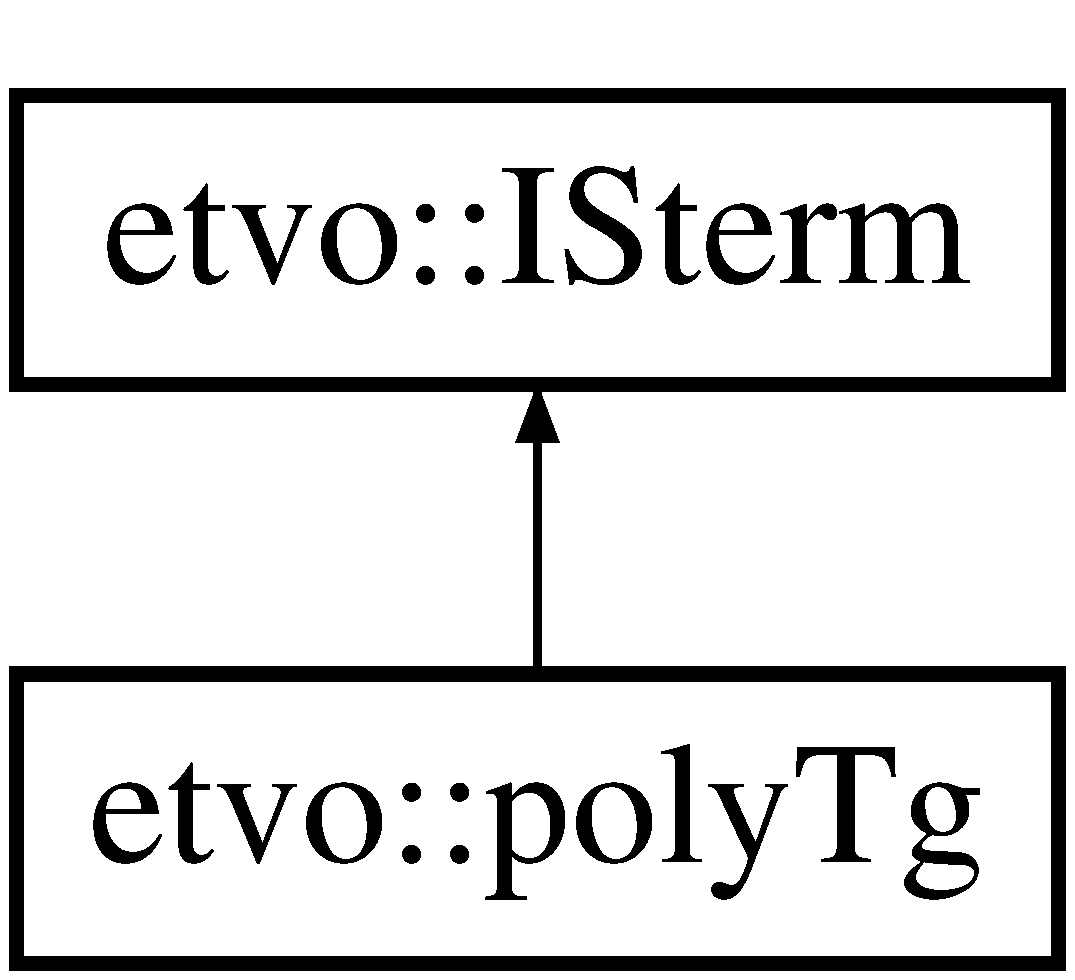
\includegraphics[height=2.000000cm]{classetvo_1_1poly_tg}
\end{center}
\end{figure}
\subsection*{Public Member Functions}
\begin{DoxyCompactItemize}
\item 
\mbox{\label{classetvo_1_1poly_tg_a2a8af2fbcc8c693da0ea6fe607425050}} 
\textbf{ poly\+Tg} ()
\begin{DoxyCompactList}\small\item\em initialised with Epsilon element \end{DoxyCompactList}\item 
\mbox{\label{classetvo_1_1poly_tg_a928e4668cc41d89ec75bed1916126844}} 
\textbf{ poly\+Tg} (const \textbf{ Tg} \&m)
\begin{DoxyCompactList}\small\item\em initialised with one monomial m \end{DoxyCompactList}\item 
\mbox{\label{classetvo_1_1poly_tg_a50e4daeebaee06eab2a85b58f02c33bd}} 
\textbf{ poly\+Tg} (bool Top\+NotE)
\begin{DoxyCompactList}\small\item\em specific initialization \+: poly\+Tg(true) set to Top, poly\+Tg(false) set to E \end{DoxyCompactList}\item 
\textbf{ poly\+Tg} (const std\+::vector$<$ \textbf{ Tg} $>$ \&v)
\item 
\mbox{\label{classetvo_1_1poly_tg_a975989073b41ed58289e26f88384ae1b}} 
\textbf{ poly} {\bfseries to\+Poly} () const
\item 
\mbox{\label{classetvo_1_1poly_tg_ad4832eafe1f24976e7a4af5fe1572f38}} 
\textbf{ poly\+Tg} {\bfseries operator+} (const \textbf{ poly\+Tg} \&p) const
\item 
\mbox{\label{classetvo_1_1poly_tg_aff37a8770f4bba79cf16cbe14960c78f}} 
\textbf{ poly\+Tg} {\bfseries oplus} (const \textbf{ poly\+Tg} \&p) const
\item 
\mbox{\label{classetvo_1_1poly_tg_a2468f9b4b3f77db0c292d4c5b73c0865}} 
\textbf{ poly\+Tg} {\bfseries oplus\+CD} (const \textbf{ poly\+Tg} \&p) const
\item 
\mbox{\label{classetvo_1_1poly_tg_ab378beddfc62f797ebca0fa2f0e689b4}} 
\textbf{ poly\+Tg} {\bfseries operator+} (const \textbf{ Tg} \&m) const
\item 
\mbox{\label{classetvo_1_1poly_tg_a49c66b6e3edd626cf7ceae3b6dd3550a}} 
void {\bfseries add} (const \textbf{ Tg} \&m)
\item 
\mbox{\label{classetvo_1_1poly_tg_ad48e68a8201c1425e354f0ad7e9f336e}} 
\textbf{ poly\+Tg} {\bfseries operator$\ast$} (const \textbf{ poly\+Tg} \&p) const
\item 
\mbox{\label{classetvo_1_1poly_tg_a4d609ff66c4a20ac89e0943706527b7a}} 
\textbf{ poly\+Tg} {\bfseries operator$\ast$} (const \textbf{ Tg} \&m) const
\item 
\mbox{\label{classetvo_1_1poly_tg_ac6b5be82fac1eb5997f663c3d57500b8}} 
\textbf{ poly\+Tg} {\bfseries otimes} (const \textbf{ poly\+Tg} \&p) const
\item 
\mbox{\label{classetvo_1_1poly_tg_aca5e926c252636b24b70774013749495}} 
\textbf{ poly\+Tg} {\bfseries otimes\+CD} (const \textbf{ poly\+Tg} \&p) const
\item 
\mbox{\label{classetvo_1_1poly_tg_a4ca680095a6866f15c87e1a379a9a2c2}} 
\textbf{ poly\+Tg} {\bfseries inf} (const \textbf{ poly\+Tg} \&p) const
\item 
\mbox{\label{classetvo_1_1poly_tg_ae7837fd345fc6c4b1df49eef3089c074}} 
\textbf{ poly\+Tg} {\bfseries inf\+CD} (const \textbf{ poly\+Tg} \&p) const
\item 
\mbox{\label{classetvo_1_1poly_tg_a7ef54630db2fbca4d4bbba2489ebcb5a}} 
\textbf{ poly\+Tg} {\bfseries lfrac} (const \textbf{ poly\+Tg} \&p) const
\item 
\mbox{\label{classetvo_1_1poly_tg_a83e333cef3abfb93e37ba3a4e2776e31}} 
\textbf{ poly\+Tg} {\bfseries lfrac\+CD} (const \textbf{ poly\+Tg} \&p) const
\item 
\mbox{\label{classetvo_1_1poly_tg_afdba8adf6afd9ff57cbfe48f81ff1943}} 
\textbf{ poly\+Tg} {\bfseries lfrac} (const \textbf{ Tg} \&m) const
\item 
\mbox{\label{classetvo_1_1poly_tg_a062da90558d45cee0286705596ab46b3}} 
\textbf{ poly\+Tg} {\bfseries rfrac} (const \textbf{ poly\+Tg} \&p) const
\item 
\mbox{\label{classetvo_1_1poly_tg_ab0a32c65e528f248133277bb84e61c44}} 
\textbf{ poly\+Tg} {\bfseries rfrac\+CD} (const \textbf{ poly\+Tg} \&p) const
\item 
\mbox{\label{classetvo_1_1poly_tg_a3fd2e8652d18796cfc5fb9357b3bee9a}} 
\textbf{ poly\+Tg} {\bfseries rfrac} (const \textbf{ Tg} \&m) const
\item 
\mbox{\label{classetvo_1_1poly_tg_ab9847846eb0e65dc880105b50fc6bbb1}} 
bool {\bfseries operator==} (const \textbf{ poly\+Tg} \&) const
\item 
\mbox{\label{classetvo_1_1poly_tg_ab8905fa00e46a4cff74b2208a289dc3b}} 
bool {\bfseries operator!=} (const \textbf{ poly\+Tg} \&) const
\item 
\mbox{\label{classetvo_1_1poly_tg_a832f566f31b3eb69ac6ada4151dd2918}} 
bool {\bfseries operator$<$=} (const \textbf{ poly\+Tg} \&) const
\item 
\mbox{\label{classetvo_1_1poly_tg_a2afebb6c24e0340274c492aedb2b3891}} 
bool {\bfseries operator$>$=} (const \textbf{ poly\+Tg} \&) const
\item 
\mbox{\label{classetvo_1_1poly_tg_a406bb20f078d0d6bd75681b731cde0e1}} 
\textbf{ poly\+Tg} {\bfseries transient\+Star} (int Tmax) const
\item 
\mbox{\label{classetvo_1_1poly_tg_a4716aa7465d14557e05fdaf9a1cbe3ae}} 
\textbf{ Tg} {\bfseries get\+First\+Dif} (const \textbf{ poly\+Tg} \&p) const
\item 
\mbox{\label{classetvo_1_1poly_tg_af71afc37d9ae1972ac358deae0bf6718}} 
void {\bfseries canon} ()
\item 
\mbox{\label{classetvo_1_1poly_tg_a07e3c591d93a632740f3715163ccd85c}} 
bool {\bfseries is\+Canon} () const
\item 
\mbox{\label{classetvo_1_1poly_tg_ad1e05beb69d77950d949d4cd64f1cce9}} 
\textbf{ Tg} {\bfseries operator[$\,$]} (unsigned idx) const
\item 
\mbox{\label{classetvo_1_1poly_tg_a28fd04bf07b85f6b822851733f2f072b}} 
unsigned int {\bfseries size} () const
\item 
\mbox{\label{classetvo_1_1poly_tg_a35ed69de3267caad83f470e52c96490d}} 
std\+::string {\bfseries to\+String} () const
\item 
\mbox{\label{classetvo_1_1poly_tg_ac603ac9159afb366e665269389b59e19}} 
std\+::string {\bfseries to\+String\+As\+Delta\+Var} () const
\item 
\mbox{\label{classetvo_1_1poly_tg_a29a61a6e25b9456aa8017ca978142085}} 
bool {\bfseries isE} () const
\item 
\mbox{\label{classetvo_1_1poly_tg_a6c94e201777977e2c9c0f93fb28c5fdd}} 
void {\bfseries get\+Max\+Gain} (unsigned int \&mb) const
\item 
\mbox{\label{classetvo_1_1poly_tg_a6177fd39c618c44a0607ad3055f96a0b}} 
void {\bfseries get\+Lcm\+Gain} (unsigned int \&mb) const
\item 
\mbox{\label{classetvo_1_1poly_tg_a8152a998bdd57600bcccdc4e7351a0b4}} 
unsigned int {\bfseries get\+Max\+Gain} () const
\item 
\mbox{\label{classetvo_1_1poly_tg_ab059f45ea77668982b27ea54b2765850}} 
unsigned int {\bfseries get\+Lcm\+Gain} () const
\item 
\mbox{\label{classetvo_1_1poly_tg_ac1113c779b38f055ee7156c6e34b0027}} 
unsigned {\bfseries get\+Periodicity} () const
\item 
\mbox{\label{classetvo_1_1poly_tg_a905bce66900cfdda17113a758bb4e399}} 
std\+::vector$<$ \textbf{ Tg} $>$ {\bfseries get\+Terms} () const
\item 
\mbox{\label{classetvo_1_1poly_tg_a002102c43a58d476beb268dee90ff9c8}} 
void {\bfseries remove\+Term} (unsigned idx)
\item 
\mbox{\label{classetvo_1_1poly_tg_ae132401e1413b749c97321431011fd3b}} 
\textbf{ matrix}$<$ \textbf{ poly} $>$ {\bfseries get\+Core} (unsigned ratio=1) const
\item 
\mbox{\label{classetvo_1_1poly_tg_a5acb9acdf83b131565f7e5d54fd76c5f}} 
\textbf{ matrix}$<$ \textbf{ poly} $>$ {\bfseries get\+Core\+Max} (unsigned ratio=1) const
\item 
\mbox{\label{classetvo_1_1poly_tg_a552150cc8c3ed3660a5dff4479c310fa}} 
void \textbf{ to\+Pov} (\textbf{ graphic\+P\+R\+::\+Pov\+Ray} \&pov, \textbf{ graphic\+P\+R\+::\+Pov\+Ray\+::\+Color} c)
\begin{DoxyCompactList}\small\item\em used in the creation of P\+O\+V-\/\+Ray script for a \doxyref{poly\+Tg}{p.}{classetvo_1_1poly_tg} object \end{DoxyCompactList}\end{DoxyCompactItemize}
\subsection*{Static Public Member Functions}
\begin{DoxyCompactItemize}
\item 
\mbox{\label{classetvo_1_1poly_tg_a5f7395bd2481043ad99fa713b17a52e9}} 
static \textbf{ poly\+Tg} \textbf{ Epsilon} ()
\begin{DoxyCompactList}\small\item\em Epsilon element. \end{DoxyCompactList}\item 
\mbox{\label{classetvo_1_1poly_tg_a5a78cab1afd2e18277c07c55fbca56f0}} 
static \textbf{ poly\+Tg} \textbf{ Top} ()
\begin{DoxyCompactList}\small\item\em Top element. \end{DoxyCompactList}\item 
\mbox{\label{classetvo_1_1poly_tg_ad2491872bc57e5869ab116817bdb94eb}} 
static \textbf{ poly\+Tg} \textbf{ E} ()
\begin{DoxyCompactList}\small\item\em neutral element \end{DoxyCompactList}\item 
\mbox{\label{classetvo_1_1poly_tg_a1b30c521af4534637fb72b25efe05d1a}} 
static \textbf{ poly\+Tg} {\bfseries to\+Poly\+Tg} (const \textbf{ poly} \&p)
\item 
\mbox{\label{classetvo_1_1poly_tg_a11be9a40a80f7d0f27171120e2917016}} 
static \textbf{ poly\+Tg} {\bfseries otimes} (const \textbf{ Tg} \&m, const \textbf{ poly\+Tg} \&p)
\item 
\mbox{\label{classetvo_1_1poly_tg_a75b26d317a10e238b384e70aad3f754f}} 
static \textbf{ etvo\+::matrix}$<$ \textbf{ poly} $>$ {\bfseries get\+MatN} (unsigned size)
\item 
\mbox{\label{classetvo_1_1poly_tg_a44cf96af7fbce586bdf3a9d1d7b384dc}} 
static \textbf{ poly\+Tg} {\bfseries core\+To\+Poly\+Tg} (const \textbf{ matrix}$<$ \textbf{ poly} $>$ \&core)
\item 
\mbox{\label{classetvo_1_1poly_tg_a8cee080792864121009ce47d0c34f1dc}} 
static \textbf{ poly\+Tg} \textbf{ to\+Causal} (const \textbf{ poly\+Tg} \&s)
\begin{DoxyCompactList}\small\item\em returns the projection of p into the set of causal series in T[[g]] (not reliable yet) \end{DoxyCompactList}\end{DoxyCompactItemize}
\subsection*{Additional Inherited Members}


\subsection{Detailed Description}
Class for polynomials in the semiring T[[g]]. 

epsilon and top element exist.

\begin{DoxyAuthor}{Author}
BC LH JT L\+A\+R\+IS 
\end{DoxyAuthor}
\begin{DoxyVersion}{Version}
2.\+0 
\end{DoxyVersion}


\subsection{Constructor \& Destructor Documentation}
\mbox{\label{classetvo_1_1poly_tg_a084bffc1ed74986e413364b3a1a6272b}} 
\index{etvo\+::poly\+Tg@{etvo\+::poly\+Tg}!poly\+Tg@{poly\+Tg}}
\index{poly\+Tg@{poly\+Tg}!etvo\+::poly\+Tg@{etvo\+::poly\+Tg}}
\subsubsection{poly\+Tg()}
{\footnotesize\ttfamily etvo\+::poly\+Tg\+::poly\+Tg (\begin{DoxyParamCaption}\item[{const std\+::vector$<$ \textbf{ Tg} $>$ \&}]{v }\end{DoxyParamCaption})}

initialization to a polynomial created from a collection of \doxyref{Tg}{p.}{classetvo_1_1_tg} terms w.\+g$^\wedge$n. The initialization leads to a canonical form where \doxyref{Tg}{p.}{classetvo_1_1_tg} terms are sorted 

The documentation for this class was generated from the following files\+:\begin{DoxyCompactItemize}
\item 
F\+:/\+U\+A Box/\+Dev\+Soft/etvo\+I\+I\+I/etvo21/etvo/series\+Tg/poly\+Tg.\+h\item 
F\+:/\+U\+A Box/\+Dev\+Soft/etvo\+I\+I\+I/etvo21/etvo/series\+Tg/poly\+Tg.\+cpp\end{DoxyCompactItemize}

\section{graphic\+PR\+:\+:Pov\+Ray Class Reference}
\label{classgraphic_p_r_1_1_pov_ray}\index{graphic\+P\+R\+::\+Pov\+Ray@{graphic\+P\+R\+::\+Pov\+Ray}}


Used to generate P\+O\+V-\/\+Ray scripts to draw 3D descriptions of poly\+Ed and poly\+Tg objects.  




{\ttfamily \#include $<$Pov\+Ray.\+h$>$}

\subsection*{Classes}
\begin{DoxyCompactItemize}
\item 
class \textbf{ Color}
\begin{DoxyCompactList}\small\item\em the script description of a color in P\+O\+V-\/\+Ray \end{DoxyCompactList}\item 
class \textbf{ Point}
\begin{DoxyCompactList}\small\item\em the script description of a point in P\+O\+V-\/\+Ray \end{DoxyCompactList}\end{DoxyCompactItemize}
\subsection*{Public Member Functions}
\begin{DoxyCompactItemize}
\item 
\mbox{\label{classgraphic_p_r_1_1_pov_ray_a7bb3dd07e8c0fffa7c70103d485a8d85}} 
\textbf{ Pov\+Ray} (const std\+::string \&str\+File\+Name)
\begin{DoxyCompactList}\small\item\em For a script description stored into the file named str\+File\+Name. \end{DoxyCompactList}\item 
\mbox{\label{classgraphic_p_r_1_1_pov_ray_ac3c935e83d1846955d7880e8921298b6}} 
void \textbf{ Axis\+Ed} ()
\begin{DoxyCompactList}\small\item\em Script for Axis creation for Ed elements. \end{DoxyCompactList}\item 
\mbox{\label{classgraphic_p_r_1_1_pov_ray_a3ba88d53d0d008ca267e56b6086b2055}} 
void \textbf{ Axis\+Tg} ()
\begin{DoxyCompactList}\small\item\em Script for Axis creation for Tg elements. \end{DoxyCompactList}\item 
\mbox{\label{classgraphic_p_r_1_1_pov_ray_ab14560a1b081a77055ddae70532d2c59}} 
void \textbf{ Pov\+\_\+\+Start\+Ed} ()
\begin{DoxyCompactList}\small\item\em Script header for Ed elements. \end{DoxyCompactList}\item 
\mbox{\label{classgraphic_p_r_1_1_pov_ray_af5b7b58da1303c3a9ddd8acea217ebf4}} 
void \textbf{ Pov\+\_\+\+Start\+Tg} ()
\begin{DoxyCompactList}\small\item\em Script header for Tg elements. \end{DoxyCompactList}\item 
\mbox{\label{classgraphic_p_r_1_1_pov_ray_a35ea6876eade87363f8970d4028b8b06}} 
void \textbf{ Pov\+\_\+\+End} ()
\begin{DoxyCompactList}\small\item\em Script closure. \end{DoxyCompactList}\item 
\mbox{\label{classgraphic_p_r_1_1_pov_ray_ab9be91bf3f5c20d6b22ba52a1613ce85}} 
void \textbf{ Save\+To\+File} ()
\begin{DoxyCompactList}\small\item\em Save the script into the file. \end{DoxyCompactList}\item 
\mbox{\label{classgraphic_p_r_1_1_pov_ray_a3c77578ed0a72b3ee7c37f3a7ad6eabe}} 
void {\bfseries Box} (\textbf{ Point} pA, \textbf{ Point} pB, \textbf{ Color} c)
\item 
\mbox{\label{classgraphic_p_r_1_1_pov_ray_a6bd3bbecca0b15620e76ccd13ddf74f1}} 
void {\bfseries Sphere} (\textbf{ Point} centre, float rayon, \textbf{ Color} c)
\item 
\mbox{\label{classgraphic_p_r_1_1_pov_ray_aaf00c01d3ea2b157ecc84cd442849d2c}} 
void {\bfseries Cylinder} (\textbf{ Point} pA, \textbf{ Point} pB, float rayon, \textbf{ Color} c)
\item 
\mbox{\label{classgraphic_p_r_1_1_pov_ray_a63f9ea3b52142759255e52a86bd26002}} 
void {\bfseries Face\+XY} (\textbf{ Point} pA, \textbf{ Point} pB)
\item 
\mbox{\label{classgraphic_p_r_1_1_pov_ray_ad23cc44a05b58c1999b12d6b89410459}} 
void {\bfseries FaceZ} (\textbf{ Point} pA, \textbf{ Point} pB)
\end{DoxyCompactItemize}
\subsection*{Public Attributes}
\begin{DoxyCompactItemize}
\item 
\mbox{\label{classgraphic_p_r_1_1_pov_ray_a71fca23628a32a631cc56198477450ae}} 
\textbf{ Point} \textbf{ Location\+Camera}
\begin{DoxyCompactList}\small\item\em Camera location in the scene. \end{DoxyCompactList}\item 
\mbox{\label{classgraphic_p_r_1_1_pov_ray_aa635deb7d40ef1b7df025f3f06f8897c}} 
\textbf{ Point} \textbf{ Camera\+Look\+At}
\begin{DoxyCompactList}\small\item\em \doxyref{Point}{p.}{classgraphic_p_r_1_1_pov_ray_1_1_point} observed by the Camera into the scene. \end{DoxyCompactList}\item 
\mbox{\label{classgraphic_p_r_1_1_pov_ray_a896f26b8097b5a550d8382d84286a73b}} 
\textbf{ Color} {\bfseries C\+Surface}
\item 
\mbox{\label{classgraphic_p_r_1_1_pov_ray_a321ea0510260db58196a8c9b7b675ab7}} 
int {\bfseries xmin}
\item 
\mbox{\label{classgraphic_p_r_1_1_pov_ray_a78b6e35f2d3ef5aeda6ba34486561cde}} 
int {\bfseries ymax}
\item 
\mbox{\label{classgraphic_p_r_1_1_pov_ray_a2fd172af17b917c197f3b7c963a423ff}} 
int {\bfseries zmin}
\item 
\mbox{\label{classgraphic_p_r_1_1_pov_ray_aa599a848834234f67d47cf695e42290a}} 
int {\bfseries xmax}
\item 
\mbox{\label{classgraphic_p_r_1_1_pov_ray_ac6210b84744668777aec1053facad7d0}} 
int {\bfseries zmax}
\item 
\mbox{\label{classgraphic_p_r_1_1_pov_ray_ac656bc8673c6b4850c8993a4c290664e}} 
int {\bfseries ymin}
\item 
\mbox{\label{classgraphic_p_r_1_1_pov_ray_a35528c2d9c457b03070e15fd1d31ab6a}} 
std\+::string {\bfseries file\+Name\+Pov\+Ray}
\item 
\mbox{\label{classgraphic_p_r_1_1_pov_ray_ab4d8d117059ee71c728c77de11e56e01}} 
std\+::strstream {\bfseries ss}
\end{DoxyCompactItemize}


\subsection{Detailed Description}
Used to generate P\+O\+V-\/\+Ray scripts to draw 3D descriptions of poly\+Ed and poly\+Tg objects. 

\begin{DoxyAuthor}{Author}
BC LH JT L\+A\+R\+IS 
\end{DoxyAuthor}
\begin{DoxyVersion}{Version}
2.\+0 
\end{DoxyVersion}


The documentation for this class was generated from the following files\+:\begin{DoxyCompactItemize}
\item 
F\+:/\+U\+A Box/\+Dev\+Soft/etvo\+I\+I\+I/etvo21/etvo/grafic/Pov\+Ray.\+h\item 
F\+:/\+U\+A Box/\+Dev\+Soft/etvo\+I\+I\+I/etvo21/etvo/grafic/Pov\+Ray.\+cpp\end{DoxyCompactItemize}

\hypertarget{classmmgd_1_1serie}{}\section{mmgd\+:\+:serie Class Reference}
\label{classmmgd_1_1serie}\index{mmgd\+::serie@{mmgd\+::serie}}
Inheritance diagram for mmgd\+:\+:serie\+:\begin{figure}[H]
\begin{center}
\leavevmode
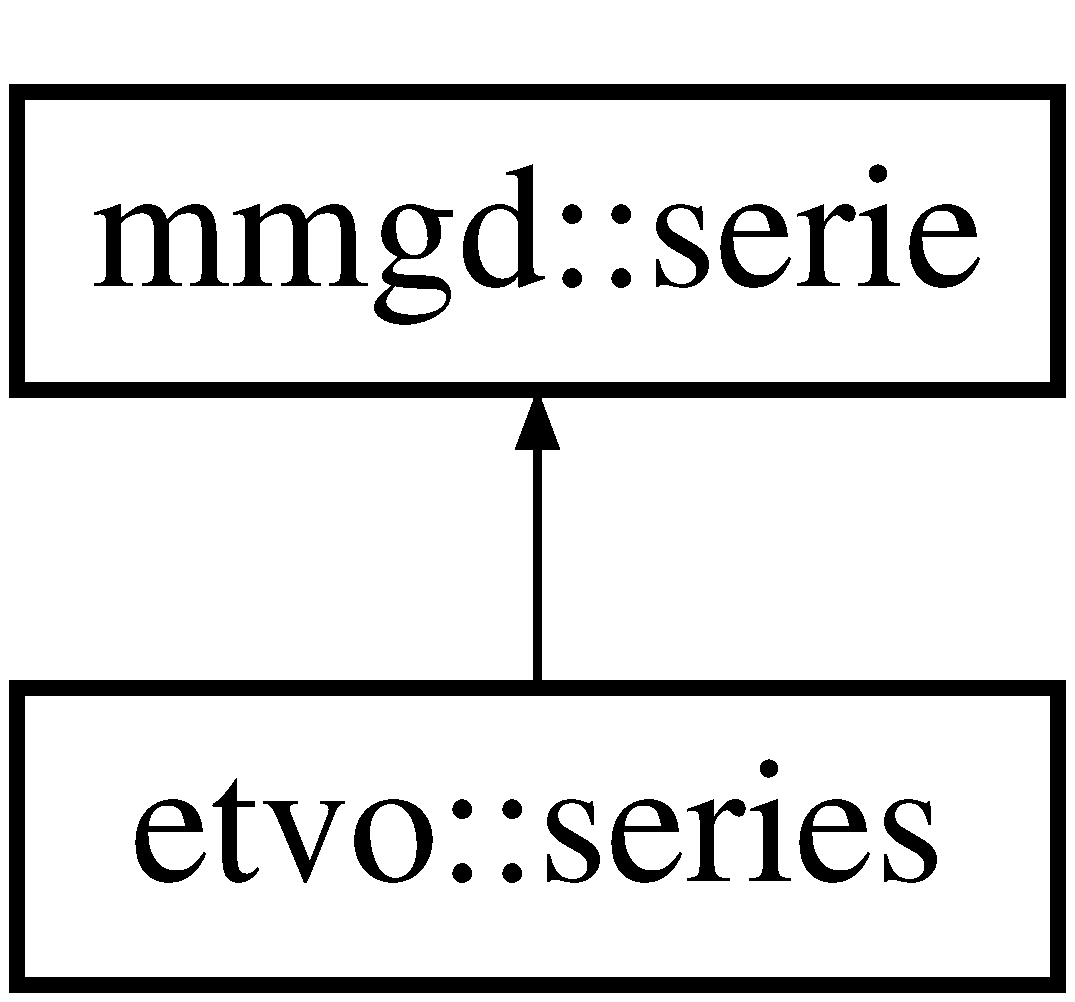
\includegraphics[height=2.000000cm]{classmmgd_1_1serie}
\end{center}
\end{figure}
\subsection*{Public Member Functions}
\begin{DoxyCompactItemize}
\item 
\mbox{\Hypertarget{classmmgd_1_1serie_aaa97a51daa7e06a231be806a84bd6073}\label{classmmgd_1_1serie_aaa97a51daa7e06a231be806a84bd6073}} 
{\bfseries serie} (const \mbox{\hyperlink{classmmgd_1_1serie}{serie}} \&)
\item 
\mbox{\Hypertarget{classmmgd_1_1serie_a2e5e176ba9944ac572e1999018e44886}\label{classmmgd_1_1serie_a2e5e176ba9944ac572e1999018e44886}} 
{\bfseries serie} (const \mbox{\hyperlink{classmmgd_1_1poly}{poly}} \&p1, const \mbox{\hyperlink{classmmgd_1_1poly}{poly}} \&q1, \mbox{\hyperlink{classmmgd_1_1gd}{gd}} \&r1)
\item 
\mbox{\Hypertarget{classmmgd_1_1serie_a4725a58c8ea4de37d2cdd88dd5b4c914}\label{classmmgd_1_1serie_a4725a58c8ea4de37d2cdd88dd5b4c914}} 
{\bfseries serie} (\mbox{\hyperlink{classmmgd_1_1poly}{poly}} \&p)
\item 
\mbox{\Hypertarget{classmmgd_1_1serie_a33e8a0a46077473352724801e10b3cf6}\label{classmmgd_1_1serie_a33e8a0a46077473352724801e10b3cf6}} 
{\bfseries serie} (\mbox{\hyperlink{classmmgd_1_1gd}{gd}} \&gd1)
\item 
\mbox{\Hypertarget{classmmgd_1_1serie_af3813bfd7099de4e1b0493dc310bd3fc}\label{classmmgd_1_1serie_af3813bfd7099de4e1b0493dc310bd3fc}} 
{\bfseries serie} (unsigned int np1, unsigned int nq1, \mbox{\hyperlink{classmmgd_1_1gd}{gd}} $\ast$p1, \mbox{\hyperlink{classmmgd_1_1gd}{gd}} $\ast$q1, \mbox{\hyperlink{classmmgd_1_1gd}{gd}} \&r1)
\item 
\mbox{\Hypertarget{classmmgd_1_1serie_a38fbdc0f684b65730903fcc2a75c2e06}\label{classmmgd_1_1serie_a38fbdc0f684b65730903fcc2a75c2e06}} 
\mbox{\hyperlink{classmmgd_1_1poly}{poly}} \& {\bfseries getp} (void)
\item 
\mbox{\Hypertarget{classmmgd_1_1serie_a67c4d214b2e02022f54ff8ff63e657f9}\label{classmmgd_1_1serie_a67c4d214b2e02022f54ff8ff63e657f9}} 
\mbox{\hyperlink{classmmgd_1_1poly}{poly}} \& {\bfseries getq} (void)
\item 
\mbox{\Hypertarget{classmmgd_1_1serie_a0650364b2ecc501864fa6e684053aa57}\label{classmmgd_1_1serie_a0650364b2ecc501864fa6e684053aa57}} 
\mbox{\hyperlink{classmmgd_1_1gd}{gd}} \& {\bfseries getr} (void)
\item 
\mbox{\Hypertarget{classmmgd_1_1serie_a066f2b3c24ff28b1b771040c7e01166e}\label{classmmgd_1_1serie_a066f2b3c24ff28b1b771040c7e01166e}} 
\mbox{\hyperlink{classmmgd_1_1serie}{serie}} \& {\bfseries operator=} (const \mbox{\hyperlink{classmmgd_1_1serie}{serie}} \&serie1)
\item 
\mbox{\Hypertarget{classmmgd_1_1serie_a2f14a188cfab4354429d9f0f87a82e58}\label{classmmgd_1_1serie_a2f14a188cfab4354429d9f0f87a82e58}} 
\mbox{\hyperlink{classmmgd_1_1serie}{serie}} \& {\bfseries operator=} (const \mbox{\hyperlink{classmmgd_1_1gd}{gd}} \&gd1)
\item 
\mbox{\Hypertarget{classmmgd_1_1serie_a21cca4fee933ae71f605215b13a612ae}\label{classmmgd_1_1serie_a21cca4fee933ae71f605215b13a612ae}} 
\mbox{\hyperlink{classmmgd_1_1serie}{serie}} \& {\bfseries operator=} (const \mbox{\hyperlink{classmmgd_1_1poly}{poly}} \&p1)
\item 
\mbox{\Hypertarget{classmmgd_1_1serie_a3ec7bfdba701b17e56c055e0a9486b6e}\label{classmmgd_1_1serie_a3ec7bfdba701b17e56c055e0a9486b6e}} 
void {\bfseries init} (\mbox{\hyperlink{classmmgd_1_1poly}{poly}} \&p1, \mbox{\hyperlink{classmmgd_1_1poly}{poly}} \&q1, \mbox{\hyperlink{classmmgd_1_1gd}{gd}} \&r1)
\item 
\mbox{\Hypertarget{classmmgd_1_1serie_ac01a3e0aea64486c264500293c6313d6}\label{classmmgd_1_1serie_ac01a3e0aea64486c264500293c6313d6}} 
void {\bfseries init} (unsigned int, unsigned int, \mbox{\hyperlink{classmmgd_1_1gd}{gd}} $\ast$, \mbox{\hyperlink{classmmgd_1_1gd}{gd}} $\ast$, \mbox{\hyperlink{classmmgd_1_1gd}{gd}} \&)
\item 
\mbox{\Hypertarget{classmmgd_1_1serie_a15d0c0636e2cf65ee8af81def95d0242}\label{classmmgd_1_1serie_a15d0c0636e2cf65ee8af81def95d0242}} 
void {\bfseries init} (\mbox{\hyperlink{classmmgd_1_1gd}{gd}} \&pgd1, \mbox{\hyperlink{classmmgd_1_1gd}{gd}} \&qgd1, \mbox{\hyperlink{classmmgd_1_1gd}{gd}} \&r1)
\item 
\mbox{\Hypertarget{classmmgd_1_1serie_a1485f36c62d4a6d3c5861c12219d28e2}\label{classmmgd_1_1serie_a1485f36c62d4a6d3c5861c12219d28e2}} 
void {\bfseries init} (\mbox{\hyperlink{classmmgd_1_1poly}{poly}} \&p1, \mbox{\hyperlink{classmmgd_1_1gd}{gd}} \&qgd1, \mbox{\hyperlink{classmmgd_1_1gd}{gd}} \&r1)
\item 
\mbox{\Hypertarget{classmmgd_1_1serie_a63454c770de7d4ee7f0216c21183574b}\label{classmmgd_1_1serie_a63454c770de7d4ee7f0216c21183574b}} 
void {\bfseries init} (\mbox{\hyperlink{classmmgd_1_1gd}{gd}} \&pgd1, \mbox{\hyperlink{classmmgd_1_1poly}{poly}} \&q1, \mbox{\hyperlink{classmmgd_1_1gd}{gd}} \&r1)
\item 
\mbox{\Hypertarget{classmmgd_1_1serie_a37939ffcb52ec8f82a45c54e34b8d3fe}\label{classmmgd_1_1serie_a37939ffcb52ec8f82a45c54e34b8d3fe}} 
void {\bfseries canon} ()
\item 
\mbox{\Hypertarget{classmmgd_1_1serie_a1d28f3f8c8f4a4f5e7b3cf17102faf25}\label{classmmgd_1_1serie_a1d28f3f8c8f4a4f5e7b3cf17102faf25}} 
int {\bfseries operator==} (\mbox{\hyperlink{classmmgd_1_1serie}{serie}} \&)
\end{DoxyCompactItemize}
\subsection*{Static Public Attributes}
\begin{DoxyCompactItemize}
\item 
\mbox{\Hypertarget{classmmgd_1_1serie_a5b098609ed451a16502695db01e95543}\label{classmmgd_1_1serie_a5b098609ed451a16502695db01e95543}} 
static \mbox{\hyperlink{classmmgd_1_1serie}{serie}} {\bfseries eps}
\end{DoxyCompactItemize}
\subsection*{Friends}
\begin{DoxyCompactItemize}
\item 
\mbox{\Hypertarget{classmmgd_1_1serie_ab5c16b5ec4f47cf21bc40d7a8ed334ba}\label{classmmgd_1_1serie_ab5c16b5ec4f47cf21bc40d7a8ed334ba}} 
std\+::ostream \& {\bfseries operator$<$$<$} (std\+::ostream \&flot, \mbox{\hyperlink{classmmgd_1_1serie}{serie}} \&serie1)
\item 
\mbox{\Hypertarget{classmmgd_1_1serie_aa30553ecd514ac08baab9da517a1634b}\label{classmmgd_1_1serie_aa30553ecd514ac08baab9da517a1634b}} 
std\+::fstream \& {\bfseries operator$<$$<$} (std\+::fstream \&flot, \mbox{\hyperlink{classmmgd_1_1serie}{serie}} \&serie1)
\item 
\mbox{\Hypertarget{classmmgd_1_1serie_a5cdfc5f944baf6a0d58154edf0289bd7}\label{classmmgd_1_1serie_a5cdfc5f944baf6a0d58154edf0289bd7}} 
\mbox{\hyperlink{classmmgd_1_1serie}{serie}} {\bfseries oplus} (\mbox{\hyperlink{classmmgd_1_1serie}{serie}} \&, \mbox{\hyperlink{classmmgd_1_1serie}{serie}} \&)
\item 
\mbox{\Hypertarget{classmmgd_1_1serie_a8cefe99b16b97b3b2259c1a7a41bdec2}\label{classmmgd_1_1serie_a8cefe99b16b97b3b2259c1a7a41bdec2}} 
\mbox{\hyperlink{classmmgd_1_1serie}{serie}} {\bfseries oplus} (\mbox{\hyperlink{classmmgd_1_1poly}{poly}} \&, \mbox{\hyperlink{classmmgd_1_1serie}{serie}} \&)
\item 
\mbox{\Hypertarget{classmmgd_1_1serie_a785a2830a23c8b9df7fbd48a063d3233}\label{classmmgd_1_1serie_a785a2830a23c8b9df7fbd48a063d3233}} 
\mbox{\hyperlink{classmmgd_1_1serie}{serie}} {\bfseries oplus} (\mbox{\hyperlink{classmmgd_1_1serie}{serie}} \&, \mbox{\hyperlink{classmmgd_1_1poly}{poly}} \&)
\item 
\mbox{\Hypertarget{classmmgd_1_1serie_a1e07a6e300fb9cbe0d6852e497b3cf2f}\label{classmmgd_1_1serie_a1e07a6e300fb9cbe0d6852e497b3cf2f}} 
\mbox{\hyperlink{classmmgd_1_1serie}{serie}} {\bfseries oplus} (\mbox{\hyperlink{classmmgd_1_1gd}{gd}} \&, \mbox{\hyperlink{classmmgd_1_1serie}{serie}} \&)
\item 
\mbox{\Hypertarget{classmmgd_1_1serie_ae3797d1df8139dea71783da93a19db37}\label{classmmgd_1_1serie_ae3797d1df8139dea71783da93a19db37}} 
\mbox{\hyperlink{classmmgd_1_1serie}{serie}} {\bfseries oplus} (\mbox{\hyperlink{classmmgd_1_1serie}{serie}} \&, \mbox{\hyperlink{classmmgd_1_1gd}{gd}} \&)
\item 
\mbox{\Hypertarget{classmmgd_1_1serie_aea7881b4435b831b601498506d6f0b81}\label{classmmgd_1_1serie_aea7881b4435b831b601498506d6f0b81}} 
\mbox{\hyperlink{classmmgd_1_1serie}{serie}} {\bfseries otimes} (\mbox{\hyperlink{classmmgd_1_1serie}{serie}} \&, \mbox{\hyperlink{classmmgd_1_1serie}{serie}} \&)
\item 
\mbox{\Hypertarget{classmmgd_1_1serie_ac420e254d3fbdecfa4c845352efceae0}\label{classmmgd_1_1serie_ac420e254d3fbdecfa4c845352efceae0}} 
\mbox{\hyperlink{classmmgd_1_1serie}{serie}} {\bfseries otimes} (\mbox{\hyperlink{classmmgd_1_1poly}{poly}} \&pol1, \mbox{\hyperlink{classmmgd_1_1serie}{serie}} \&s2)
\item 
\mbox{\Hypertarget{classmmgd_1_1serie_a2ce30e8ff131fe98008b9e8846518a64}\label{classmmgd_1_1serie_a2ce30e8ff131fe98008b9e8846518a64}} 
\mbox{\hyperlink{classmmgd_1_1serie}{serie}} {\bfseries otimes} (\mbox{\hyperlink{classmmgd_1_1serie}{serie}} \&s2, \mbox{\hyperlink{classmmgd_1_1poly}{poly}} \&pol1)
\item 
\mbox{\Hypertarget{classmmgd_1_1serie_a64dd80055a1485aa4188d3e51b65f327}\label{classmmgd_1_1serie_a64dd80055a1485aa4188d3e51b65f327}} 
\mbox{\hyperlink{classmmgd_1_1serie}{serie}} {\bfseries otimes} (\mbox{\hyperlink{classmmgd_1_1gd}{gd}} \&gd1, \mbox{\hyperlink{classmmgd_1_1serie}{serie}} \&s2)
\item 
\mbox{\Hypertarget{classmmgd_1_1serie_adae673cecde6bd03cc153ca190902664}\label{classmmgd_1_1serie_adae673cecde6bd03cc153ca190902664}} 
\mbox{\hyperlink{classmmgd_1_1serie}{serie}} {\bfseries otimes} (\mbox{\hyperlink{classmmgd_1_1serie}{serie}} \&s2, \mbox{\hyperlink{classmmgd_1_1gd}{gd}} \&gd1)
\item 
\mbox{\Hypertarget{classmmgd_1_1serie_ab39087f51b76a3f107d9a9470e53a588}\label{classmmgd_1_1serie_ab39087f51b76a3f107d9a9470e53a588}} 
\mbox{\hyperlink{classmmgd_1_1serie}{serie}} {\bfseries star} (\mbox{\hyperlink{classmmgd_1_1poly}{poly}} poly1)
\item 
\mbox{\Hypertarget{classmmgd_1_1serie_a373238aae64f359f9dd07639e18f2450}\label{classmmgd_1_1serie_a373238aae64f359f9dd07639e18f2450}} 
\mbox{\hyperlink{classmmgd_1_1serie}{serie}} {\bfseries star} (\mbox{\hyperlink{classmmgd_1_1gd}{gd}} \&r1)
\item 
\mbox{\Hypertarget{classmmgd_1_1serie_ad896bd7caaabe6801478307c7d792f65}\label{classmmgd_1_1serie_ad896bd7caaabe6801478307c7d792f65}} 
\mbox{\hyperlink{classmmgd_1_1serie}{serie}} {\bfseries star} (\mbox{\hyperlink{classmmgd_1_1serie}{serie}} \&s1)
\item 
\mbox{\Hypertarget{classmmgd_1_1serie_a2d481e6996673bb393e494e9597f9149}\label{classmmgd_1_1serie_a2d481e6996673bb393e494e9597f9149}} 
\mbox{\hyperlink{classmmgd_1_1serie}{serie}} {\bfseries inf} (\mbox{\hyperlink{classmmgd_1_1serie}{serie}} \&s1, \mbox{\hyperlink{classmmgd_1_1serie}{serie}} \&s2)
\item 
\mbox{\hyperlink{classmmgd_1_1serie}{serie}} \mbox{\hyperlink{classmmgd_1_1serie_ae529c9c97ff0829cde0be6b234952d67}{inf}} (\mbox{\hyperlink{classmmgd_1_1serie}{serie}} \&s1, \mbox{\hyperlink{classmmgd_1_1poly}{poly}} \&p2)
\item 
\mbox{\Hypertarget{classmmgd_1_1serie_a6da306502d5cbecbda9e28e464beb459}\label{classmmgd_1_1serie_a6da306502d5cbecbda9e28e464beb459}} 
\mbox{\hyperlink{classmmgd_1_1serie}{serie}} {\bfseries inf} (\mbox{\hyperlink{classmmgd_1_1poly}{poly}} \&p1, \mbox{\hyperlink{classmmgd_1_1serie}{serie}} \&s2)
\item 
\mbox{\Hypertarget{classmmgd_1_1serie_a02bcc7dd146114b8b79a0e6864cc7ad4}\label{classmmgd_1_1serie_a02bcc7dd146114b8b79a0e6864cc7ad4}} 
\mbox{\hyperlink{classmmgd_1_1serie}{serie}} {\bfseries inf} (\mbox{\hyperlink{classmmgd_1_1gd}{gd}} \&, \mbox{\hyperlink{classmmgd_1_1serie}{serie}} \&)
\item 
\mbox{\Hypertarget{classmmgd_1_1serie_ae5191750772678d2a419a573059e4514}\label{classmmgd_1_1serie_ae5191750772678d2a419a573059e4514}} 
\mbox{\hyperlink{classmmgd_1_1serie}{serie}} {\bfseries inf} (\mbox{\hyperlink{classmmgd_1_1serie}{serie}} \&, \mbox{\hyperlink{classmmgd_1_1gd}{gd}} \&)
\item 
\mbox{\Hypertarget{classmmgd_1_1serie_a003b5ee69741b8c166467d26f6574c25}\label{classmmgd_1_1serie_a003b5ee69741b8c166467d26f6574c25}} 
\mbox{\hyperlink{classmmgd_1_1serie}{serie}} {\bfseries frac} (\mbox{\hyperlink{classmmgd_1_1serie}{serie}} \&s1, \mbox{\hyperlink{classmmgd_1_1serie}{serie}} \&s2)
\item 
\mbox{\Hypertarget{classmmgd_1_1serie_a225fb5e2b9dd1f597226271a090a4298}\label{classmmgd_1_1serie_a225fb5e2b9dd1f597226271a090a4298}} 
\mbox{\hyperlink{classmmgd_1_1serie}{serie}} {\bfseries frac} (\mbox{\hyperlink{classmmgd_1_1serie}{serie}} \&s1, \mbox{\hyperlink{classmmgd_1_1gd}{gd}} \&gd2)
\item 
\mbox{\Hypertarget{classmmgd_1_1serie_a1ada807b04afe2bc3299b5e3ffa3f506}\label{classmmgd_1_1serie_a1ada807b04afe2bc3299b5e3ffa3f506}} 
\mbox{\hyperlink{classmmgd_1_1serie}{serie}} {\bfseries frac} (\mbox{\hyperlink{classmmgd_1_1serie}{serie}} \&s1, \mbox{\hyperlink{classmmgd_1_1poly}{poly}} \&poly1)
\item 
\mbox{\Hypertarget{classmmgd_1_1serie_a96a942e6263b0d9e099db5db3a6c0d9b}\label{classmmgd_1_1serie_a96a942e6263b0d9e099db5db3a6c0d9b}} 
\mbox{\hyperlink{classmmgd_1_1serie}{serie}} {\bfseries odot} (\mbox{\hyperlink{classmmgd_1_1serie}{serie}} \&, \mbox{\hyperlink{classmmgd_1_1serie}{serie}} \&)
\item 
\mbox{\Hypertarget{classmmgd_1_1serie_ac5d2d6f470449131209b2ecae26749fa}\label{classmmgd_1_1serie_ac5d2d6f470449131209b2ecae26749fa}} 
\mbox{\hyperlink{classmmgd_1_1serie}{serie}} {\bfseries odot} (\mbox{\hyperlink{classmmgd_1_1serie}{serie}} \&s1, \mbox{\hyperlink{classmmgd_1_1poly}{poly}} \&p2)
\item 
\mbox{\Hypertarget{classmmgd_1_1serie_ae07cb54d85919e3aa78c6ea6a38007b7}\label{classmmgd_1_1serie_ae07cb54d85919e3aa78c6ea6a38007b7}} 
\mbox{\hyperlink{classmmgd_1_1serie}{serie}} {\bfseries odot} (\mbox{\hyperlink{classmmgd_1_1poly}{poly}} \&p1, \mbox{\hyperlink{classmmgd_1_1serie}{serie}} \&s2)
\item 
\mbox{\Hypertarget{classmmgd_1_1serie_ac2ac2502c6f1f27a35fbeeea04fb4c16}\label{classmmgd_1_1serie_ac2ac2502c6f1f27a35fbeeea04fb4c16}} 
\mbox{\hyperlink{classmmgd_1_1serie}{serie}} {\bfseries fracodotsharp} (\mbox{\hyperlink{classmmgd_1_1serie}{serie}} \&, \mbox{\hyperlink{classmmgd_1_1serie}{serie}} \&)
\item 
\mbox{\Hypertarget{classmmgd_1_1serie_abcdcbf3dc5fe1c1257a5c3ff5cbc0945}\label{classmmgd_1_1serie_abcdcbf3dc5fe1c1257a5c3ff5cbc0945}} 
\mbox{\hyperlink{classmmgd_1_1serie}{serie}} {\bfseries fracodotflat} (\mbox{\hyperlink{classmmgd_1_1serie}{serie}} \&, \mbox{\hyperlink{classmmgd_1_1serie}{serie}} \&)
\item 
\mbox{\Hypertarget{classmmgd_1_1serie_a96ec45b632f274cbe3e36ed354c2fb59}\label{classmmgd_1_1serie_a96ec45b632f274cbe3e36ed354c2fb59}} 
\mbox{\hyperlink{classmmgd_1_1serie}{serie}} {\bfseries Dualfrac} (\mbox{\hyperlink{classmmgd_1_1serie}{serie}} \&s1, \mbox{\hyperlink{classmmgd_1_1gd}{gd}} \&gd2)
\item 
\mbox{\Hypertarget{classmmgd_1_1serie_a2c82a0b41c08782a6bfc3412746ee102}\label{classmmgd_1_1serie_a2c82a0b41c08782a6bfc3412746ee102}} 
\mbox{\hyperlink{classmmgd_1_1serie}{serie}} {\bfseries prcaus} (\mbox{\hyperlink{classmmgd_1_1serie}{serie}} \&)
\end{DoxyCompactItemize}


\subsection{Friends And Related Function Documentation}
\mbox{\Hypertarget{classmmgd_1_1serie_ae529c9c97ff0829cde0be6b234952d67}\label{classmmgd_1_1serie_ae529c9c97ff0829cde0be6b234952d67}} 
\index{mmgd\+::serie@{mmgd\+::serie}!inf@{inf}}
\index{inf@{inf}!mmgd\+::serie@{mmgd\+::serie}}
\subsubsection{\texorpdfstring{inf}{inf}}
{\footnotesize\ttfamily \mbox{\hyperlink{classmmgd_1_1serie}{serie}} inf (\begin{DoxyParamCaption}\item[{\mbox{\hyperlink{classmmgd_1_1serie}{serie}} \&}]{s1,  }\item[{\mbox{\hyperlink{classmmgd_1_1poly}{poly}} \&}]{p2 }\end{DoxyParamCaption})\hspace{0.3cm}{\ttfamily [friend]}}

inf d\textquotesingle{}une s�ie et d\textquotesingle{}un polyn�e 

The documentation for this class was generated from the following files\+:\begin{DoxyCompactItemize}
\item 
etvo/minmaxgd/serie.\+h\item 
etvo/minmaxgd/serie.\+cpp\end{DoxyCompactItemize}

\section{etvo\+:\+:series Class Reference}
\label{classetvo_1_1series}\index{etvo\+::series@{etvo\+::series}}


Wrapper class to \doxyref{mmgd\+::serie}{p.}{classmmgd_1_1serie} from Min\+Max\+GD library.  




{\ttfamily \#include $<$series\+Wrapper.\+h$>$}

Inheritance diagram for etvo\+:\+:series\+:\begin{figure}[H]
\begin{center}
\leavevmode
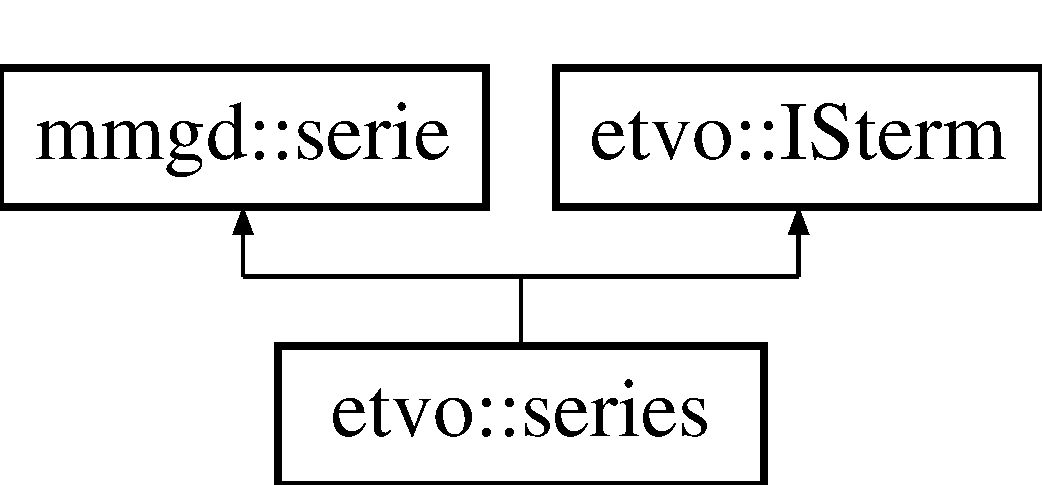
\includegraphics[height=2.000000cm]{classetvo_1_1series}
\end{center}
\end{figure}
\subsection*{Public Member Functions}
\begin{DoxyCompactItemize}
\item 
\mbox{\label{classetvo_1_1series_af9042df4357269780732fd48247eec91}} 
bool {\bfseries isE} () const
\item 
\mbox{\label{classetvo_1_1series_acdf41b448e13bbf522e9de4755153be4}} 
bool {\bfseries is\+Poly} () const
\item 
\mbox{\label{classetvo_1_1series_a3a104d731521a0e9a8f6820baa3e9ae5}} 
bool {\bfseries is\+Degenerate} () const
\item 
\mbox{\label{classetvo_1_1series_a62c43a051c9c9508ef441d50edac9ea5}} 
\textbf{ series} ()
\begin{DoxyCompactList}\small\item\em default constructor \+: epsilon series p=eps q=eps r=g0.\+d0 \end{DoxyCompactList}\item 
\mbox{\label{classetvo_1_1series_a2fb51387e5e2c9033bb64e097dfafd51}} 
\textbf{ series} (const \textbf{ gd} \&)
\begin{DoxyCompactList}\small\item\em constructor \+: set a series from only one monomial (uses the next constructor) \end{DoxyCompactList}\item 
\mbox{\label{classetvo_1_1series_abd4d7be395e14b12bd8f3de30f122539}} 
\textbf{ series} (const \textbf{ poly} \&)
\begin{DoxyCompactList}\small\item\em constructor \+: set a series from a polynomial \end{DoxyCompactList}\item 
\mbox{\label{classetvo_1_1series_a6dcc6b366be40756f3fff156a725f341}} 
\textbf{ series} (const \textbf{ mmgd\+::serie} \&s)
\begin{DoxyCompactList}\small\item\em constructor \+: set a etvo\+I\+I\+::series from a mmgg\+::serie \end{DoxyCompactList}\item 
\mbox{\label{classetvo_1_1series_a02032180329f48133d41e5143d97711a}} 
\textbf{ series} (const \textbf{ poly} \&p, const \textbf{ poly} \&q, const \textbf{ gd} \&r)
\begin{DoxyCompactList}\small\item\em constructor \+: set a etvo\+I\+I\+::series from p+q.r$\ast$ representation \end{DoxyCompactList}\item 
\mbox{\label{classetvo_1_1series_a2fe114ea671d2fa6d60cbb347e36a3bf}} 
\textbf{ poly} \textbf{ getP} () const
\begin{DoxyCompactList}\small\item\em gives polynomial p (as etvo\+I\+I\+::poly) \end{DoxyCompactList}\item 
\mbox{\label{classetvo_1_1series_ac133165b16e18d843fa912ee4997278e}} 
\textbf{ poly} \textbf{ getQ} () const
\begin{DoxyCompactList}\small\item\em gives polynomial q (as etvo\+I\+I\+::poly) \end{DoxyCompactList}\item 
\mbox{\label{classetvo_1_1series_a3c4ad8943e890e1cc2e85ce848467ae0}} 
\textbf{ gd} \textbf{ getR} () const
\begin{DoxyCompactList}\small\item\em gives monomial r (as etvo\+I\+I\+::gd) \end{DoxyCompactList}\item 
\mbox{\label{classetvo_1_1series_ac01af20daccd40a5dada22bf0661125e}} 
bool {\bfseries operator!=} (const \textbf{ series} \&s) const
\item 
\mbox{\label{classetvo_1_1series_a92c26c932f402c8cbe695c5e24bacaf8}} 
bool {\bfseries operator==} (const \textbf{ series} \&s) const
\item 
\mbox{\label{classetvo_1_1series_a361b862af945267e7e9ac1d168f6fd76}} 
bool {\bfseries operator$<$=} (const \textbf{ series} \&s) const
\item 
\mbox{\label{classetvo_1_1series_af86a7a8ad6f68e5e7f87c9001c87803c}} 
bool {\bfseries operator$>$=} (const \textbf{ series} \&s) const
\item 
\mbox{\label{classetvo_1_1series_a8ebfc000ddf2dc797aab8f418ab5c380}} 
\textbf{ series} \textbf{ operator+} (const \textbf{ series} \&s) const
\begin{DoxyCompactList}\small\item\em computes the sum of two series in Min\+Max[[g,d]] \end{DoxyCompactList}\item 
\mbox{\label{classetvo_1_1series_a1cdfbad469208751d81713a688a8cd6b}} 
\textbf{ series} \textbf{ operator$\ast$} (const \textbf{ series} \&s) const
\begin{DoxyCompactList}\small\item\em computes the product of two series in Min\+Max[[g,d]] \end{DoxyCompactList}\item 
\mbox{\label{classetvo_1_1series_a18a89048a319f4decaa9537932a348a0}} 
\textbf{ series} \textbf{ inf} (const \textbf{ series} \&s) const
\begin{DoxyCompactList}\small\item\em computes the infimum of two series in Min\+Max[[g,d]] \end{DoxyCompactList}\item 
\mbox{\label{classetvo_1_1series_a50e448835f9b642a9afcfa4bd794aaf0}} 
\textbf{ series} \textbf{ star} () const
\begin{DoxyCompactList}\small\item\em computes the Kleene star of a series in Min\+Max[[g,d]] \end{DoxyCompactList}\item 
\mbox{\label{classetvo_1_1series_a76da40b12dc11c9a9cdb1fe20a072609}} 
\textbf{ series} \textbf{ lfrac} (const \textbf{ series} \&s) const
\begin{DoxyCompactList}\small\item\em equiv. frac because the product is commutative \end{DoxyCompactList}\item 
\mbox{\label{classetvo_1_1series_aad8c2ee6cba5028a2f3ae5e33b7a69e7}} 
\textbf{ series} \textbf{ rfrac} (const \textbf{ series} \&s) const
\begin{DoxyCompactList}\small\item\em equiv. frac because the product is commutative \end{DoxyCompactList}\item 
\mbox{\label{classetvo_1_1series_adc565ed1e17f23aa96b8d2137580f115}} 
\textbf{ series} \textbf{ frac} (const \textbf{ series} \&s) const
\begin{DoxyCompactList}\small\item\em s1.\+frac(s2) is the greatest series x s.\+t. s2.\+x $<$= s1 \end{DoxyCompactList}\item 
\mbox{\label{classetvo_1_1series_a68e52557163917584687f4e104d69cc1}} 
\textbf{ series} \textbf{ frac} (const \textbf{ gd} \&m) const
\begin{DoxyCompactList}\small\item\em s1.\+frac(g2.\+dt) is the greatest series x s.\+t. gn.\+dt.\+x $<$= s1 \end{DoxyCompactList}\item 
\mbox{\label{classetvo_1_1series_a37d4dd0629adbf8320cd6e83fe535bd2}} 
\textbf{ series} \textbf{ frac} (const \textbf{ poly} \&p) const
\begin{DoxyCompactList}\small\item\em s1.\+frac(p) is the greatest series x s.\+t. p.\+x $<$= s1 \end{DoxyCompactList}\item 
\mbox{\label{classetvo_1_1series_aea1e95f83e8612f4bac27cdc25d59071}} 
\textbf{ series} \textbf{ prcaus} () const
\begin{DoxyCompactList}\small\item\em gives the causal projection of the current series. \end{DoxyCompactList}\item 
\mbox{\label{classetvo_1_1series_a178950f62416cbf31292c4d35238467f}} 
std\+::string \textbf{ To\+String} () const
\begin{DoxyCompactList}\small\item\em gives a string giving the description of a series in a format g1.\+d2+g2.d3+(g4.\+d5+g6.d7).[g3.\+d3]$\ast$ \end{DoxyCompactList}\end{DoxyCompactItemize}
\subsection*{Static Public Member Functions}
\begin{DoxyCompactItemize}
\item 
\mbox{\label{classetvo_1_1series_aedddfac41864e41c1fe87b099b8b96b3}} 
static \textbf{ series} \textbf{ Epsilon} ()
\begin{DoxyCompactList}\small\item\em gives the epsilon series \end{DoxyCompactList}\item 
\mbox{\label{classetvo_1_1series_a5d51766db365fdeb43bcb5491c3dd315}} 
static \textbf{ series} \textbf{ E} ()
\begin{DoxyCompactList}\small\item\em gives the series e=g0.\+d0 \end{DoxyCompactList}\item 
\mbox{\label{classetvo_1_1series_ab7b66bb192070a7e3b49ea85ac876c94}} 
static \textbf{ series} \textbf{ Top} ()
\begin{DoxyCompactList}\small\item\em gives the top series T \end{DoxyCompactList}\end{DoxyCompactItemize}
\subsection*{Additional Inherited Members}


\subsection{Detailed Description}
Wrapper class to \doxyref{mmgd\+::serie}{p.}{classmmgd_1_1serie} from Min\+Max\+GD library. 

Class for ultimately periodic series s=p + q [g$^\wedge$n.d$^\wedge$t]$\ast$ in Min\+Max[[g,d]], where p and q are polynomials

An epsilon and a top series exists

\begin{DoxyAuthor}{Author}
BC LH JT L\+A\+R\+IS 
\end{DoxyAuthor}
\begin{DoxyVersion}{Version}
2.\+0 
\end{DoxyVersion}


The documentation for this class was generated from the following files\+:\begin{DoxyCompactItemize}
\item 
F\+:/\+U\+A Box/\+Dev\+Soft/etvo\+I\+I\+I/etvo21/etvo/wrapper\+M\+M\+G\+D/\textbf{ series\+Wrapper.\+h}\item 
F\+:/\+U\+A Box/\+Dev\+Soft/etvo\+I\+I\+I/etvo21/etvo/wrapper\+M\+M\+G\+D/series\+Wrapper.\+cpp\end{DoxyCompactItemize}

\section{etvo\+:\+:series\+Ed Class Reference}
\label{classetvo_1_1series_ed}\index{etvo\+::series\+Ed@{etvo\+::series\+Ed}}


Class for ultimately-\/periodic series in the semiring E[[d]]. In a general way, the series are described by two standard (canonical) forms s=p+q.r$\ast$=p\textquotesingle{}+r\textquotesingle{}$\ast$.q\textquotesingle{} where p,p\textquotesingle{},q,q\textquotesingle{} are polynomials in E[[d]] and r/r\textquotesingle{} are \doxyref{etvo\+::gd}{p.}{classetvo_1_1gd} terms (in Min\+Max[[g,d]]).  




{\ttfamily \#include $<$series\+Ed.\+h$>$}

Inheritance diagram for etvo\+:\+:series\+Ed\+:\begin{figure}[H]
\begin{center}
\leavevmode
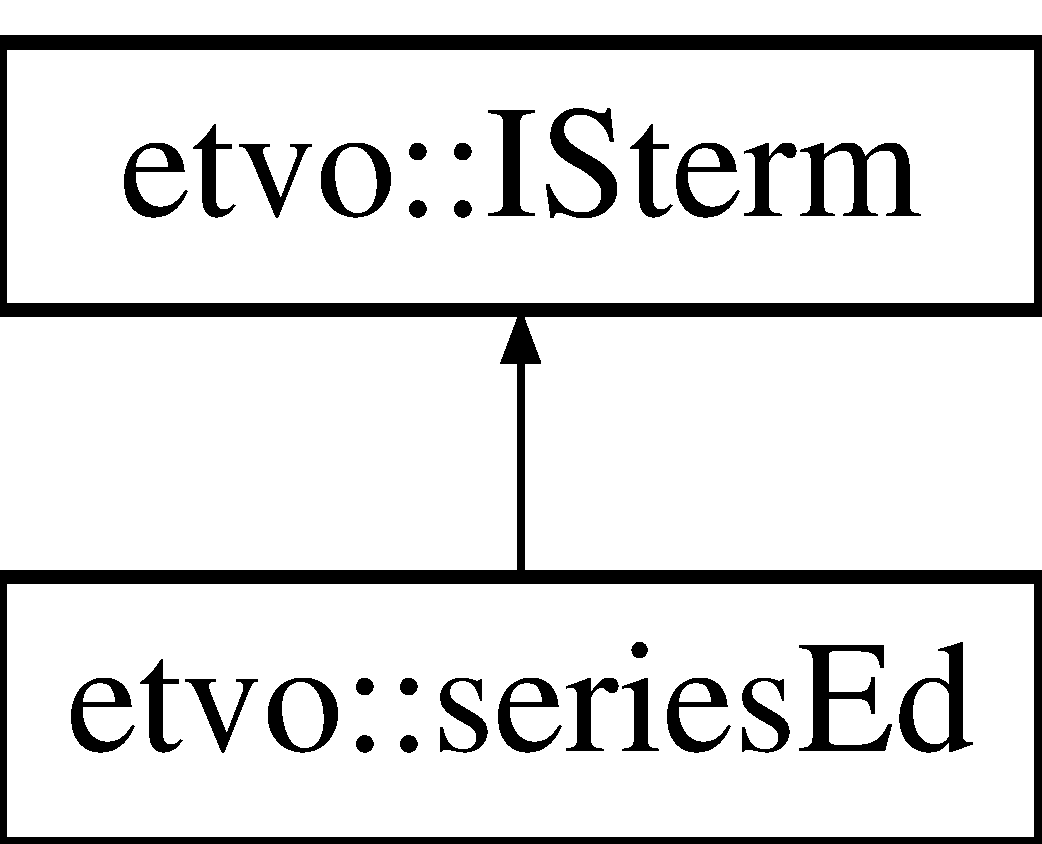
\includegraphics[height=2.000000cm]{classetvo_1_1series_ed}
\end{center}
\end{figure}
\subsection*{Public Member Functions}
\begin{DoxyCompactItemize}
\item 
\mbox{\label{classetvo_1_1series_ed_a31dadcdb993fdf20b003b48688062394}} 
\textbf{ series\+Ed} ()
\begin{DoxyCompactList}\small\item\em Default initialization \+: epsilon (p=eps q=eps r=g1.\+d0) \end{DoxyCompactList}\item 
\textbf{ series\+Ed} (bool Top\+NotE)
\item 
\mbox{\label{classetvo_1_1series_ed_a3e9489a6a6ee291a72c20f4c7f5ee3af}} 
\textbf{ series\+Ed} (const \textbf{ Ed} \&m)
\begin{DoxyCompactList}\small\item\em Initialization of a \doxyref{series\+Ed}{p.}{classetvo_1_1series_ed} from \doxyref{Ed}{p.}{classetvo_1_1_ed} term m (p=eps q=m r=g1.\+d0) \end{DoxyCompactList}\item 
\mbox{\label{classetvo_1_1series_ed_a260d739e1ee23af4ec99ac8d3b30381b}} 
\textbf{ series\+Ed} (const \textbf{ poly\+Ed} \&q)
\begin{DoxyCompactList}\small\item\em Initialization of a \doxyref{series\+Ed}{p.}{classetvo_1_1series_ed} from \doxyref{poly\+Ed}{p.}{classetvo_1_1poly_ed} term q (p=eps q=q r=g1.\+d0) \end{DoxyCompactList}\item 
\textbf{ series\+Ed} (const \textbf{ poly\+Ed} \&p, const \textbf{ poly\+Ed} \&q, long n, long t, bool right=true)
\item 
\textbf{ series\+Ed} (const \textbf{ poly\+Ed} \&p, const \textbf{ poly\+Ed} \&q, const \textbf{ gd} \&r, bool right=1)
\item 
\mbox{\label{classetvo_1_1series_ed_a0f4b0324f57dd434d0590c070f72b8b1}} 
bool \textbf{ is\+Right\+Form} () const
\begin{DoxyCompactList}\small\item\em check if the current series in Right form \end{DoxyCompactList}\item 
\mbox{\label{classetvo_1_1series_ed_a81818d9e8c36b69a246fa537b6933d14}} 
bool \textbf{ is\+Left\+Form} () const
\begin{DoxyCompactList}\small\item\em check if the current series in Left form \end{DoxyCompactList}\item 
\mbox{\label{classetvo_1_1series_ed_a7be58a01e1bec68d9c42e3bb6c10b01f}} 
bool \textbf{ is\+Polynomial} () const
\begin{DoxyCompactList}\small\item\em check if it is a polynomial \end{DoxyCompactList}\item 
\mbox{\label{classetvo_1_1series_ed_a61e6624c51d6fa3e513538bb6762363e}} 
bool \textbf{ is\+Proper} () const
\begin{DoxyCompactList}\small\item\em check if it is in proper form \end{DoxyCompactList}\item 
\mbox{\label{classetvo_1_1series_ed_a4536bd7bc11d56bd3509618b2a8090bf}} 
bool \textbf{ isE} () const
\begin{DoxyCompactList}\small\item\em check if it is a neutral \doxyref{series\+Ed}{p.}{classetvo_1_1series_ed} \end{DoxyCompactList}\item 
\mbox{\label{classetvo_1_1series_ed_a565be244fa8e0a6721c3d470c762ac1f}} 
void \textbf{ canon} ()
\begin{DoxyCompactList}\small\item\em leads to the canonical left or right form (the simplest proper form) \end{DoxyCompactList}\item 
\mbox{\label{classetvo_1_1series_ed_a3f52bb9e67d00acbdac6487a106b8d27}} 
void \textbf{ to\+Right} ()
\begin{DoxyCompactList}\small\item\em to Right form \end{DoxyCompactList}\item 
\mbox{\label{classetvo_1_1series_ed_a5d30fbb5746801ad323267ce719618d9}} 
void \textbf{ to\+Left} ()
\begin{DoxyCompactList}\small\item\em to Left form \end{DoxyCompactList}\item 
\mbox{\label{classetvo_1_1series_ed_abceaaec1fc51bde4c3cd5c0fced618c9}} 
\textbf{ poly\+Ed} \textbf{ getP} () const
\begin{DoxyCompactList}\small\item\em getter returning p \end{DoxyCompactList}\item 
\mbox{\label{classetvo_1_1series_ed_a656ac64645516ce9aa8c4c8d0355494c}} 
\textbf{ poly\+Ed} \textbf{ getQ} () const
\begin{DoxyCompactList}\small\item\em getter returning q \end{DoxyCompactList}\item 
\mbox{\label{classetvo_1_1series_ed_ac7b0a765a311b8f2811f71b2cb488cd1}} 
\textbf{ gd} \textbf{ getR} () const
\begin{DoxyCompactList}\small\item\em getter returning r \end{DoxyCompactList}\item 
\mbox{\label{classetvo_1_1series_ed_aa8b226dc9f12575519c930c82348ea0b}} 
std\+::vector$<$ \textbf{ series} $>$ \textbf{ to\+Impulse\+Response} () const
\begin{DoxyCompactList}\small\item\em returns the response to I,g1.\+I,g2.\+I ... \end{DoxyCompactList}\item 
\mbox{\label{classetvo_1_1series_ed_a8599585229b3439b53209026f8d6dd0a}} 
void \textbf{ get\+Lcm\+Gain} (unsigned int \&mu, unsigned int \&beta) const
\begin{DoxyCompactList}\small\item\em returns the Least Common multiple of gains in the terms of the current series \end{DoxyCompactList}\item 
\mbox{\label{classetvo_1_1series_ed_a2f3b7652201664e2697977f8d32000ac}} 
void \textbf{ get\+Max\+Gain} (unsigned int \&mu, unsigned int \&beta) const
\begin{DoxyCompactList}\small\item\em returns the Maximum of gains in the terms of the current series \end{DoxyCompactList}\item 
\mbox{\label{classetvo_1_1series_ed_a5d1d9392ef366b70764b64f1ee030213}} 
std\+::pair$<$ unsigned int, unsigned int $>$ \textbf{ get\+Max\+Gain} () const
\begin{DoxyCompactList}\small\item\em returns the gain as a pair (mu,beta) \end{DoxyCompactList}\item 
std\+::string \textbf{ to\+String} () const
\item 
std\+::string \textbf{ to\+String\+As\+Mu\+Var} () const
\item 
\mbox{\label{classetvo_1_1series_ed_a5da9d84a7e8c946f44711e3b93032029}} 
bool \textbf{ operator==} (const \textbf{ series\+Ed} \&s) const
\begin{DoxyCompactList}\small\item\em check equality \end{DoxyCompactList}\item 
\mbox{\label{classetvo_1_1series_ed_aedc60a13b5c648c97811758fedbb8a4e}} 
bool \textbf{ operator!=} (const \textbf{ series\+Ed} \&) const
\begin{DoxyCompactList}\small\item\em check difference \end{DoxyCompactList}\item 
\mbox{\label{classetvo_1_1series_ed_ac582288fd69a135ce9c2f60e5009763a}} 
bool \textbf{ operator$<$=} (const \textbf{ series\+Ed} \&) const
\begin{DoxyCompactList}\small\item\em check order on series \end{DoxyCompactList}\item 
\mbox{\label{classetvo_1_1series_ed_a81cc27bb6771eaceecfbb93e4168a29b}} 
bool \textbf{ operator$>$=} (const \textbf{ series\+Ed} \&) const
\begin{DoxyCompactList}\small\item\em check order on series \end{DoxyCompactList}\item 
\textbf{ series\+Ed} \textbf{ oplus} (const \textbf{ series\+Ed} \&s) const
\item 
\textbf{ series\+Ed} \textbf{ oplus} (const \textbf{ poly\+Ed} \&p) const
\item 
\mbox{\label{classetvo_1_1series_ed_ab5d476354cd91596397b3f9d70c60f50}} 
\textbf{ series\+Ed} \textbf{ otimes} (const \textbf{ series\+Ed} \&s) const
\begin{DoxyCompactList}\small\item\em product of series in E[[d]] \+: s1.\+otimes(s2) \end{DoxyCompactList}\item 
\mbox{\label{classetvo_1_1series_ed_a6a007f4b494b01191ffc761aec335643}} 
\textbf{ series\+Ed} \textbf{ otimes} (const \textbf{ Ed} \&m) const
\begin{DoxyCompactList}\small\item\em product of a series by a monomial in E[[d]] \+: s1.\+otimes(m) \end{DoxyCompactList}\item 
\mbox{\label{classetvo_1_1series_ed_a05db75c11aeb6d2d994afe56d1045f92}} 
\textbf{ series\+Ed} \textbf{ otimes} (const \textbf{ poly\+Ed} \&p) const
\begin{DoxyCompactList}\small\item\em product of a series by a polynomial in E[[d]] \+: s1.\+otimes(p) \end{DoxyCompactList}\item 
\textbf{ series\+Ed} \textbf{ operator+} (const \textbf{ series\+Ed} \&s) const
\item 
\mbox{\label{classetvo_1_1series_ed_ad64863495d5a30dad13c2c8973fead9c}} 
\textbf{ series\+Ed} \textbf{ operator$\ast$} (const \textbf{ series\+Ed} \&s) const
\begin{DoxyCompactList}\small\item\em product of series in E[[d]] \+: s1$\ast$s2 \end{DoxyCompactList}\item 
\mbox{\label{classetvo_1_1series_ed_a62d172ed81e7d07c70cac1495c695522}} 
\textbf{ series\+Ed} \textbf{ operator$\ast$} (const \textbf{ Ed} \&m) const
\begin{DoxyCompactList}\small\item\em product of a series by a monomial in E[[d]] \+: s1$\ast$m \end{DoxyCompactList}\item 
\mbox{\label{classetvo_1_1series_ed_a5dbcc25d70327828d9559317358cc51a}} 
\textbf{ series\+Ed} \textbf{ operator$\ast$} (const \textbf{ poly\+Ed} \&p) const
\begin{DoxyCompactList}\small\item\em product of a series by a polynomial in E[[d]] \+: s1$\ast$p \end{DoxyCompactList}\item 
\textbf{ series\+Ed} \textbf{ star} () const
\item 
\textbf{ series\+Ed} \textbf{ star\+Alternate} () const
\item 
\textbf{ series\+Ed} \textbf{ star\+CD} () const
\item 
\textbf{ series\+Ed} \textbf{ star\+Poly\+Based} () const
\item 
\mbox{\label{classetvo_1_1series_ed_a8e4eb3a3e75d5a463c49f1d2d2fad38d}} 
\textbf{ series\+Ed} \textbf{ lfrac} (const \textbf{ series\+Ed} \&s) const
\begin{DoxyCompactList}\small\item\em left-\/product residuation \+: s1.\+lfrac(s2) = s2 \end{DoxyCompactList}\item 
\mbox{\label{classetvo_1_1series_ed_a484dddde4ca257f9bf3b3dee3e248379}} 
\textbf{ series\+Ed} \textbf{ rfrac} (const \textbf{ series\+Ed} \&s) const
\begin{DoxyCompactList}\small\item\em right-\/product residuation \+: s1.\+rfrac(s2) = s1/s2 \end{DoxyCompactList}\item 
\mbox{\label{classetvo_1_1series_ed_a75f0bac54cfa5015a99216324abfd6db}} 
\textbf{ series\+Ed} \textbf{ otimes\+CD} (const \textbf{ series\+Ed} \&s) const
\begin{DoxyCompactList}\small\item\em operations via Core Decomposition \+: otimes \end{DoxyCompactList}\item 
\mbox{\label{classetvo_1_1series_ed_a3816015344d1867643b3f7d0cdd12a07}} 
\textbf{ series\+Ed} \textbf{ oplus\+CD} (const \textbf{ series\+Ed} \&s) const
\begin{DoxyCompactList}\small\item\em operations via Core Decomposition \+: oplus \end{DoxyCompactList}\item 
\mbox{\label{classetvo_1_1series_ed_a57d0e33121221bf50893abbd3acf6aa1}} 
\textbf{ series\+Ed} \textbf{ inf\+CD} (const \textbf{ series\+Ed} \&s) const
\begin{DoxyCompactList}\small\item\em operations via Core Decomposition \+: inf \end{DoxyCompactList}\item 
\mbox{\label{classetvo_1_1series_ed_a8b03290b1be40a5c781b17438f67de5f}} 
\textbf{ series\+Ed} \textbf{ inf} (const \textbf{ series\+Ed} \&s) const
\begin{DoxyCompactList}\small\item\em inf of series \end{DoxyCompactList}\item 
\mbox{\label{classetvo_1_1series_ed_aa1ac6321ef6deebe319fb182ce0c9f4b}} 
\textbf{ series\+Ed} \textbf{ lfrac\+CD} (const \textbf{ series\+Ed} \&s) const
\begin{DoxyCompactList}\small\item\em operations via Core Decomposition \+: lfrac \end{DoxyCompactList}\item 
\mbox{\label{classetvo_1_1series_ed_aacfb0365cbd310698b34c10bb4423550}} 
\textbf{ series\+Ed} \textbf{ rfrac\+CD} (const \textbf{ series\+Ed} \&s) const
\begin{DoxyCompactList}\small\item\em operations via Core Decomposition \+: rfrac \end{DoxyCompactList}\item 
\mbox{\label{classetvo_1_1series_ed_a8090d4177bb1226db0758f1fb28ec830}} 
\textbf{ poly\+Ed} \textbf{ get\+Poly\+Up\+To} (int deltaT) const
\begin{DoxyCompactList}\small\item\em method to develop the first terms of p+q.[r]$\ast$ or p+[r]$\ast$.q up to a given deltaT time value \end{DoxyCompactList}\item 
\mbox{\label{classetvo_1_1series_ed_ac70dfad0bac3da2eafe8bb0f3c03f587}} 
\textbf{ series} \textbf{ to\+Series} () const
\begin{DoxyCompactList}\small\item\em projection series\+Ed-\/$>$series (zero slice) \end{DoxyCompactList}\item 
\textbf{ etvo\+::matrix}$<$ \textbf{ series} $>$ \textbf{ get\+Core} (unsigned ratio=1) const
\item 
\textbf{ etvo\+::matrix}$<$ \textbf{ series} $>$ \textbf{ get\+Core\+Max} (unsigned ratio=1) const
\end{DoxyCompactItemize}
\subsection*{Static Public Member Functions}
\begin{DoxyCompactItemize}
\item 
\mbox{\label{classetvo_1_1series_ed_a8bd80bdb4362544182ab2ec0e5383c06}} 
static \textbf{ series\+Ed} \textbf{ Epsilon} ()
\begin{DoxyCompactList}\small\item\em The epsilon description of \doxyref{series\+Ed}{p.}{classetvo_1_1series_ed}. \end{DoxyCompactList}\item 
\mbox{\label{classetvo_1_1series_ed_afcd4ef0a9eea590c747997df8f42bdb5}} 
static \textbf{ series\+Ed} \textbf{ Top} ()
\begin{DoxyCompactList}\small\item\em The Top description of \doxyref{series\+Ed}{p.}{classetvo_1_1series_ed}. \end{DoxyCompactList}\item 
\mbox{\label{classetvo_1_1series_ed_af8b3bca68462681140d7773d998a1d8f}} 
static \textbf{ series\+Ed} \textbf{ E} ()
\begin{DoxyCompactList}\small\item\em The description of g0.\+d0 as \doxyref{series\+Ed}{p.}{classetvo_1_1series_ed}. \end{DoxyCompactList}\item 
static \textbf{ series\+Ed} \textbf{ oplus} (const \textbf{ poly\+Ed} \&p, const \textbf{ series\+Ed} \&s)
\item 
\mbox{\label{classetvo_1_1series_ed_a213461c266789eb06d16fd6e08dece01}} 
static \textbf{ series\+Ed} \textbf{ otimes} (const \textbf{ Ed} \&m, const \textbf{ series\+Ed} \&s)
\begin{DoxyCompactList}\small\item\em [S\+T\+A\+T\+IC] product of a monomial and a series in E[[d]] \+: series\+Ed\+::otimes(m,s) \end{DoxyCompactList}\item 
\mbox{\label{classetvo_1_1series_ed_a4ee9bee83fe0a4d06aeafbcb74e02a71}} 
static \textbf{ series\+Ed} \textbf{ otimes} (const \textbf{ poly\+Ed} \&m, const \textbf{ series\+Ed} \&s)
\begin{DoxyCompactList}\small\item\em [S\+T\+A\+T\+IC] product of a polynomial and a series in E[[d]] \+: series\+Ed\+::otimes(p,s) \end{DoxyCompactList}\item 
\mbox{\label{classetvo_1_1series_ed_a2c87c1ea77a6d55f2d18aeb07451c0f2}} 
static \textbf{ poly\+Ed} \textbf{ get\+Poly\+Up\+To} (int deltaT, const \textbf{ poly\+Ed} \&p, const \textbf{ poly\+Ed} \&q, const \textbf{ gd} \&r, bool droite=true)
\begin{DoxyCompactList}\small\item\em static function to develop the first terms of p+q.[r]$\ast$ or p+[r]$\ast$.q up to a given deltaT time value \end{DoxyCompactList}\item 
\mbox{\label{classetvo_1_1series_ed_af4e5410dd8c3bd2f3e0cb78e693f21a1}} 
static \textbf{ series\+Ed} \textbf{ to\+Causal} (const \textbf{ series\+Ed} \&s)
\begin{DoxyCompactList}\small\item\em returns the projection of s into the set of causal series in E[[d]] (not reliable yet) \end{DoxyCompactList}\item 
\mbox{\label{classetvo_1_1series_ed_a6f2beb8d017b557fc7ef03b869e2b1d3}} 
static \textbf{ series\+Ed} \textbf{ to\+Series\+Ed} (const \textbf{ series} \&s)
\begin{DoxyCompactList}\small\item\em injection series(mmgd)-\/$>$\doxyref{series\+Ed}{p.}{classetvo_1_1series_ed} \end{DoxyCompactList}\item 
\mbox{\label{classetvo_1_1series_ed_a74a7dd6beb2ab2b83722e6379119c2a9}} 
static \textbf{ series\+Ed} \textbf{ core\+To\+Series\+Ed} (const \textbf{ matrix}$<$ \textbf{ series} $>$ \&C)
\begin{DoxyCompactList}\small\item\em conversion C\+O\+RE decomposition -\/$>$ \doxyref{series\+Ed}{p.}{classetvo_1_1series_ed} \end{DoxyCompactList}\item 
\mbox{\label{classetvo_1_1series_ed_a53cc50f520ed8f63ecc7f4ed269d9047}} 
static \textbf{ etvo\+::matrix}$<$ \textbf{ series} $>$ {\bfseries get\+MatN} (unsigned size)
\end{DoxyCompactItemize}
\subsection*{Additional Inherited Members}


\subsection{Detailed Description}
Class for ultimately-\/periodic series in the semiring E[[d]]. In a general way, the series are described by two standard (canonical) forms s=p+q.r$\ast$=p\textquotesingle{}+r\textquotesingle{}$\ast$.q\textquotesingle{} where p,p\textquotesingle{},q,q\textquotesingle{} are polynomials in E[[d]] and r/r\textquotesingle{} are \doxyref{etvo\+::gd}{p.}{classetvo_1_1gd} terms (in Min\+Max[[g,d]]). 

s=p+q.r$\ast$ is called the right-\/form (because the periodic pattern is expressed with a right multiplication by r$\ast$)

s=p\textquotesingle{}+r\textquotesingle{}$\ast$.q\textquotesingle{} is called the left-\/form (because the periodic pattern is expressed with a left multiplication by r\textquotesingle{}$\ast$)

This class provides the main operations on ultimately-\/periodic series in E[[d]] such as \+:sum,product, Kleene star (when it is possible to compute the Kleene star), left/right product residuation. Some operations are possible thanks to a Core Decomposition introduced by J.\+Trunk.

The library contains also some usefull functions to swap left/right form, to obtain a projection into Min\+Max[[g,d]] (zero-\/slice projection). By using the boost library, it is also possible to express series in a string format for which a parser is given. Epsilon and Top element exist

\begin{DoxyAuthor}{Author}
BC LH JT L\+A\+R\+IS 
\end{DoxyAuthor}
\begin{DoxyVersion}{Version}
2.\+0 
\end{DoxyVersion}


\subsection{Constructor \& Destructor Documentation}
\mbox{\label{classetvo_1_1series_ed_a7c983cfef4089a4874a689dac8cababa}} 
\index{etvo\+::series\+Ed@{etvo\+::series\+Ed}!series\+Ed@{series\+Ed}}
\index{series\+Ed@{series\+Ed}!etvo\+::series\+Ed@{etvo\+::series\+Ed}}
\subsubsection{series\+Ed()\hspace{0.1cm}{\footnotesize\ttfamily [1/3]}}
{\footnotesize\ttfamily etvo\+::series\+Ed\+::series\+Ed (\begin{DoxyParamCaption}\item[{bool}]{Top\+NotE }\end{DoxyParamCaption})}

Initialization as Top (true) OR E(false) Top (p=T q=T r=g1.\+d0) E (p=eps q=g0.\+d0 r=g1.\+d0) \mbox{\label{classetvo_1_1series_ed_ac39505bea956ec81fdc4c24648b3c3bc}} 
\index{etvo\+::series\+Ed@{etvo\+::series\+Ed}!series\+Ed@{series\+Ed}}
\index{series\+Ed@{series\+Ed}!etvo\+::series\+Ed@{etvo\+::series\+Ed}}
\subsubsection{series\+Ed()\hspace{0.1cm}{\footnotesize\ttfamily [2/3]}}
{\footnotesize\ttfamily etvo\+::series\+Ed\+::series\+Ed (\begin{DoxyParamCaption}\item[{const \textbf{ poly\+Ed} \&}]{p,  }\item[{const \textbf{ poly\+Ed} \&}]{q,  }\item[{long}]{n,  }\item[{long}]{t,  }\item[{bool}]{right = {\ttfamily true} }\end{DoxyParamCaption})}

Initialization of a \doxyref{series\+Ed}{p.}{classetvo_1_1series_ed} from periodic p,q,r (right/left) form if right=true -\/$>$ s=p+q.[gn.\+dt]$\ast$ otherwise -\/$>$ s=p+[gn.\+dt]$\ast$.q \mbox{\label{classetvo_1_1series_ed_adcc3d10416984ac1adc24ddabf3c3285}} 
\index{etvo\+::series\+Ed@{etvo\+::series\+Ed}!series\+Ed@{series\+Ed}}
\index{series\+Ed@{series\+Ed}!etvo\+::series\+Ed@{etvo\+::series\+Ed}}
\subsubsection{series\+Ed()\hspace{0.1cm}{\footnotesize\ttfamily [3/3]}}
{\footnotesize\ttfamily etvo\+::series\+Ed\+::series\+Ed (\begin{DoxyParamCaption}\item[{const \textbf{ poly\+Ed} \&}]{p,  }\item[{const \textbf{ poly\+Ed} \&}]{q,  }\item[{const \textbf{ gd} \&}]{r,  }\item[{bool}]{right = {\ttfamily 1} }\end{DoxyParamCaption})}

Initialization of a \doxyref{series\+Ed}{p.}{classetvo_1_1series_ed} from periodic p,q,r (right/left) form if right=true -\/$>$ s=p+q.[r]$\ast$ otherwise -\/$>$ s=p+[r]$\ast$.q 

\subsection{Member Function Documentation}
\mbox{\label{classetvo_1_1series_ed_a65b0978f4f727b29708a5156c39cdf62}} 
\index{etvo\+::series\+Ed@{etvo\+::series\+Ed}!get\+Core@{get\+Core}}
\index{get\+Core@{get\+Core}!etvo\+::series\+Ed@{etvo\+::series\+Ed}}
\subsubsection{get\+Core()}
{\footnotesize\ttfamily \textbf{ etvo\+::matrix}$<$ \textbf{ series} $>$ etvo\+::series\+Ed\+::get\+Core (\begin{DoxyParamCaption}\item[{unsigned}]{ratio = {\ttfamily 1} }\end{DoxyParamCaption}) const}

returns the Core matrix of the current series. A ratio!=1 allows us to expand the matrix to a multiple of the basic gain. \mbox{\label{classetvo_1_1series_ed_a84034472ea37cadc7b834ccdb3646d44}} 
\index{etvo\+::series\+Ed@{etvo\+::series\+Ed}!get\+Core\+Max@{get\+Core\+Max}}
\index{get\+Core\+Max@{get\+Core\+Max}!etvo\+::series\+Ed@{etvo\+::series\+Ed}}
\subsubsection{get\+Core\+Max()}
{\footnotesize\ttfamily \textbf{ etvo\+::matrix}$<$ \textbf{ series} $>$ etvo\+::series\+Ed\+::get\+Core\+Max (\begin{DoxyParamCaption}\item[{unsigned}]{ratio = {\ttfamily 1} }\end{DoxyParamCaption}) const}

returns the maximal Core matrix of the current series. A ratio!=1 allows us to expand the matrix to a multiple of the basic gain. \mbox{\label{classetvo_1_1series_ed_a57ea848dda2da3c37fdf8625c79b0216}} 
\index{etvo\+::series\+Ed@{etvo\+::series\+Ed}!operator+@{operator+}}
\index{operator+@{operator+}!etvo\+::series\+Ed@{etvo\+::series\+Ed}}
\subsubsection{operator+()}
{\footnotesize\ttfamily \textbf{ series\+Ed} etvo\+::series\+Ed\+::operator+ (\begin{DoxyParamCaption}\item[{const \textbf{ series\+Ed} \&}]{s }\end{DoxyParamCaption}) const}

sum of series in E[[d]] \+: s1+s2 (calls oplus) Throws an exception if s1 and s2 unbalanced (different gains) \mbox{\label{classetvo_1_1series_ed_ab23342944a3abf0fa0214b4a65dbae4a}} 
\index{etvo\+::series\+Ed@{etvo\+::series\+Ed}!oplus@{oplus}}
\index{oplus@{oplus}!etvo\+::series\+Ed@{etvo\+::series\+Ed}}
\subsubsection{oplus()\hspace{0.1cm}{\footnotesize\ttfamily [1/3]}}
{\footnotesize\ttfamily \textbf{ series\+Ed} etvo\+::series\+Ed\+::oplus (\begin{DoxyParamCaption}\item[{const \textbf{ series\+Ed} \&}]{s }\end{DoxyParamCaption}) const}

sum of series in E[[d]] \+: s1.\+oplus(s2) Throws an exception if s1 and s2 unbalanced (different gains) \mbox{\label{classetvo_1_1series_ed_a794f004e9984a1942f324f7399605d47}} 
\index{etvo\+::series\+Ed@{etvo\+::series\+Ed}!oplus@{oplus}}
\index{oplus@{oplus}!etvo\+::series\+Ed@{etvo\+::series\+Ed}}
\subsubsection{oplus()\hspace{0.1cm}{\footnotesize\ttfamily [2/3]}}
{\footnotesize\ttfamily \textbf{ series\+Ed} etvo\+::series\+Ed\+::oplus (\begin{DoxyParamCaption}\item[{const \textbf{ poly\+Ed} \&}]{p }\end{DoxyParamCaption}) const}

sum of series and polynomial in E[[d]] \+: s1.\+oplus(p1) Throws an exception if s1 and p1 unbalanced (different gains) \mbox{\label{classetvo_1_1series_ed_af670d9b01ef23e6f33175d4818a98585}} 
\index{etvo\+::series\+Ed@{etvo\+::series\+Ed}!oplus@{oplus}}
\index{oplus@{oplus}!etvo\+::series\+Ed@{etvo\+::series\+Ed}}
\subsubsection{oplus()\hspace{0.1cm}{\footnotesize\ttfamily [3/3]}}
{\footnotesize\ttfamily \textbf{ series\+Ed} etvo\+::series\+Ed\+::oplus (\begin{DoxyParamCaption}\item[{const \textbf{ poly\+Ed} \&}]{p,  }\item[{const \textbf{ series\+Ed} \&}]{s }\end{DoxyParamCaption})\hspace{0.3cm}{\ttfamily [static]}}

[S\+T\+A\+T\+IC] sum of a polynomial and a series in E[[d]] \+: series\+Ed\+::oplus(p,s) Throws an exception if p and s unbalanced (different gains) \mbox{\label{classetvo_1_1series_ed_aa718fd479898554f28599f888c5c4c8b}} 
\index{etvo\+::series\+Ed@{etvo\+::series\+Ed}!star@{star}}
\index{star@{star}!etvo\+::series\+Ed@{etvo\+::series\+Ed}}
\subsubsection{star()}
{\footnotesize\ttfamily \textbf{ series\+Ed} etvo\+::series\+Ed\+::star (\begin{DoxyParamCaption}{ }\end{DoxyParamCaption}) const}

returns the Kleene star of a series in E[[d]]. Operates via a Core Decomposition of the series (see J.\+Trunk thesis) Throws an exception if the computation is not handled yet (degenerate case) \mbox{\label{classetvo_1_1series_ed_aa4ade804b79c00b6edc8b0d75be1c4da}} 
\index{etvo\+::series\+Ed@{etvo\+::series\+Ed}!star\+Alternate@{star\+Alternate}}
\index{star\+Alternate@{star\+Alternate}!etvo\+::series\+Ed@{etvo\+::series\+Ed}}
\subsubsection{star\+Alternate()}
{\footnotesize\ttfamily \textbf{ series\+Ed} etvo\+::series\+Ed\+::star\+Alternate (\begin{DoxyParamCaption}{ }\end{DoxyParamCaption}) const}

returns the Kleene star of a series in E[[d]]. A different algorithm is used (without Core Decomposition) to obtain the result. Throws an exception if the computation is not handled yet (degenerate case) \mbox{\label{classetvo_1_1series_ed_a314fe8c7f02cdcddc941dabfa8e5bb62}} 
\index{etvo\+::series\+Ed@{etvo\+::series\+Ed}!star\+CD@{star\+CD}}
\index{star\+CD@{star\+CD}!etvo\+::series\+Ed@{etvo\+::series\+Ed}}
\subsubsection{star\+C\+D()}
{\footnotesize\ttfamily \textbf{ series\+Ed} etvo\+::series\+Ed\+::star\+CD (\begin{DoxyParamCaption}{ }\end{DoxyParamCaption}) const}

returns the Kleene star of a series in E[[d]]. Operates via a Core Decomposition of the series (see J.\+Trunk thesis) \mbox{\label{classetvo_1_1series_ed_a018fa16e76e0ba91e9d1dac552103d70}} 
\index{etvo\+::series\+Ed@{etvo\+::series\+Ed}!star\+Poly\+Based@{star\+Poly\+Based}}
\index{star\+Poly\+Based@{star\+Poly\+Based}!etvo\+::series\+Ed@{etvo\+::series\+Ed}}
\subsubsection{star\+Poly\+Based()}
{\footnotesize\ttfamily \textbf{ series\+Ed} etvo\+::series\+Ed\+::star\+Poly\+Based (\begin{DoxyParamCaption}{ }\end{DoxyParamCaption}) const}

returns the star of a series by using the star of a polynomial as function. \mbox{\label{classetvo_1_1series_ed_a8ddf3e9c9d80205467eb2872709b1f13}} 
\index{etvo\+::series\+Ed@{etvo\+::series\+Ed}!to\+String@{to\+String}}
\index{to\+String@{to\+String}!etvo\+::series\+Ed@{etvo\+::series\+Ed}}
\subsubsection{to\+String()}
{\footnotesize\ttfamily std\+::string etvo\+::series\+Ed\+::to\+String (\begin{DoxyParamCaption}{ }\end{DoxyParamCaption}) const}

returns the string description of a series in E[[d]]. This format is compatible with the parser of \doxyref{series\+Ed}{p.}{classetvo_1_1series_ed} (needs boost installation) \mbox{\label{classetvo_1_1series_ed_a03b6f65ab4c82c9f4626f689918585ed}} 
\index{etvo\+::series\+Ed@{etvo\+::series\+Ed}!to\+String\+As\+Mu\+Var@{to\+String\+As\+Mu\+Var}}
\index{to\+String\+As\+Mu\+Var@{to\+String\+As\+Mu\+Var}!etvo\+::series\+Ed@{etvo\+::series\+Ed}}
\subsubsection{to\+String\+As\+Mu\+Var()}
{\footnotesize\ttfamily std\+::string etvo\+::series\+Ed\+::to\+String\+As\+Mu\+Var (\begin{DoxyParamCaption}{ }\end{DoxyParamCaption}) const}

returns the string description of a series in E[[d]] with mu$<$seq$>$ operators. This format is compatible with the parser of \doxyref{series\+Ed}{p.}{classetvo_1_1series_ed} (needs boost installation) 

The documentation for this class was generated from the following files\+:\begin{DoxyCompactItemize}
\item 
F\+:/\+U\+A Box/\+Dev\+Soft/etvo\+I\+I\+I/etvo21/etvo/series\+Ed/\textbf{ series\+Ed.\+h}\item 
F\+:/\+U\+A Box/\+Dev\+Soft/etvo\+I\+I\+I/etvo21/etvo/series\+Ed/series\+Ed.\+cpp\end{DoxyCompactItemize}

\section{etvo\+:\+:series\+Tg Class Reference}
\label{classetvo_1_1series_tg}\index{etvo\+::series\+Tg@{etvo\+::series\+Tg}}


Class for ultimately-\/periodic series in the semiring T[[g]].  




{\ttfamily \#include $<$series\+Tg.\+h$>$}

Inheritance diagram for etvo\+:\+:series\+Tg\+:\begin{figure}[H]
\begin{center}
\leavevmode
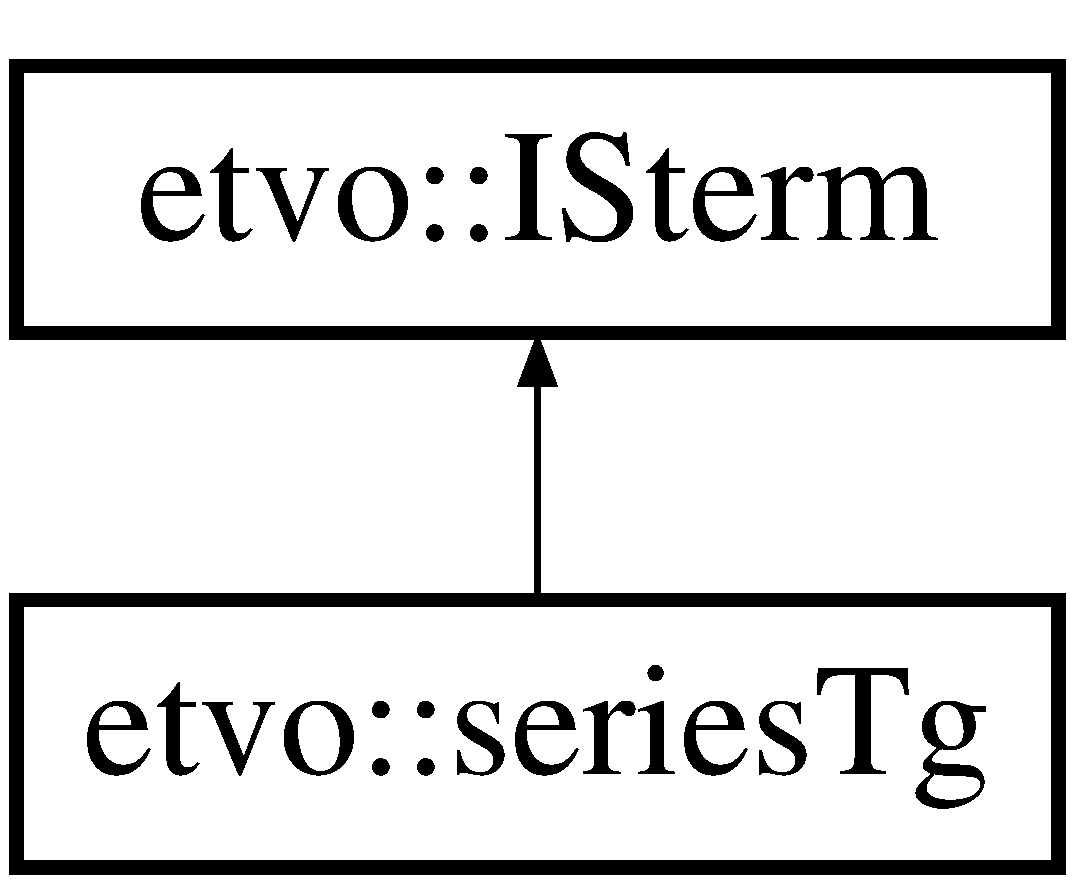
\includegraphics[height=2.000000cm]{classetvo_1_1series_tg}
\end{center}
\end{figure}
\subsection*{Public Member Functions}
\begin{DoxyCompactItemize}
\item 
\mbox{\label{classetvo_1_1series_tg_a67fe7c33eabed38affaa6c2e867481aa}} 
\textbf{ series\+Tg} ()
\begin{DoxyCompactList}\small\item\em Default initialization \+: epsilon (p=eps q=eps r=g1.\+d0) \end{DoxyCompactList}\item 
\textbf{ series\+Tg} (bool Top\+NotE)
\item 
\mbox{\label{classetvo_1_1series_tg_abfa4a629d40905e3f0c4fdc2a6ac4cc3}} 
\textbf{ series\+Tg} (const \textbf{ Tg} \&m)
\begin{DoxyCompactList}\small\item\em Initialization of a \doxyref{series\+Tg}{p.}{classetvo_1_1series_tg} from \doxyref{Tg}{p.}{classetvo_1_1_tg} term m (p=eps q=m r=g1.\+d0) \end{DoxyCompactList}\item 
\mbox{\label{classetvo_1_1series_tg_a043fffc8582e8e994fbdbf869d83c215}} 
\textbf{ series\+Tg} (const \textbf{ poly\+Tg} \&q)
\begin{DoxyCompactList}\small\item\em Initialization of a \doxyref{series\+Tg}{p.}{classetvo_1_1series_tg} from \doxyref{poly\+Tg}{p.}{classetvo_1_1poly_tg} term q (p=eps q=q r=g1.\+d0) \end{DoxyCompactList}\item 
\textbf{ series\+Tg} (const \textbf{ poly\+Tg} \&p, const \textbf{ poly\+Tg} \&q, long n, long t, bool right=true)
\item 
\textbf{ series\+Tg} (const \textbf{ poly\+Tg} \&p, const \textbf{ poly\+Tg} \&q, const \textbf{ gd} \&r, bool right=1)
\item 
\mbox{\label{classetvo_1_1series_tg_a659b0be1fef0e15a5fd1081618948572}} 
bool \textbf{ is\+Right\+Form} () const
\begin{DoxyCompactList}\small\item\em check if the current series in Right form \end{DoxyCompactList}\item 
\mbox{\label{classetvo_1_1series_tg_acce711196a87d6c2f91129fa5a96a52f}} 
bool \textbf{ is\+Left\+Form} () const
\begin{DoxyCompactList}\small\item\em check if the current series in Left form \end{DoxyCompactList}\item 
\mbox{\label{classetvo_1_1series_tg_a0918e7ac2cfa6b753b5f900a01d7dea3}} 
bool \textbf{ is\+Polynomial} () const
\begin{DoxyCompactList}\small\item\em check if it is a polynomial \end{DoxyCompactList}\item 
\mbox{\label{classetvo_1_1series_tg_aa5d7c63fa4638c094466b08c7ed968d7}} 
bool \textbf{ is\+Proper} () const
\begin{DoxyCompactList}\small\item\em check if it is in proper form \end{DoxyCompactList}\item 
\mbox{\label{classetvo_1_1series_tg_a9d36e2b96a54eabf992bc5a4bcdd44a4}} 
bool \textbf{ isE} () const
\begin{DoxyCompactList}\small\item\em check if it is a neutral \doxyref{series\+Ed}{p.}{classetvo_1_1series_ed} \end{DoxyCompactList}\item 
\mbox{\label{classetvo_1_1series_tg_a7ec38ae9488e42e8d2194bdc1b4da099}} 
void \textbf{ canon} ()
\begin{DoxyCompactList}\small\item\em leads to the canonical left or right form (the simplest proper form) \end{DoxyCompactList}\item 
\mbox{\label{classetvo_1_1series_tg_ac19fc716d7b15ee79596e36bd6aef953}} 
void \textbf{ to\+Right} ()
\begin{DoxyCompactList}\small\item\em to Right form \end{DoxyCompactList}\item 
\mbox{\label{classetvo_1_1series_tg_a410eccda4ca76790cbe1d9287c446d8b}} 
void \textbf{ to\+Left} ()
\begin{DoxyCompactList}\small\item\em to Left form \end{DoxyCompactList}\item 
\mbox{\label{classetvo_1_1series_tg_ae0dd01558c462797ff3061b52bfe2209}} 
\textbf{ poly\+Tg} \textbf{ getP} () const
\begin{DoxyCompactList}\small\item\em getter returning p \end{DoxyCompactList}\item 
\mbox{\label{classetvo_1_1series_tg_a699280593079d0da351897c82133882c}} 
\textbf{ poly\+Tg} \textbf{ getQ} () const
\begin{DoxyCompactList}\small\item\em getter returning q \end{DoxyCompactList}\item 
\mbox{\label{classetvo_1_1series_tg_ae9045a8ce85b050e251c4aa33cc589f5}} 
\textbf{ gd} \textbf{ getR} () const
\begin{DoxyCompactList}\small\item\em getter returning r \end{DoxyCompactList}\item 
std\+::string \textbf{ to\+String} () const
\item 
std\+::string \textbf{ to\+String\+As\+Delta\+Var} () const
\item 
\mbox{\label{classetvo_1_1series_tg_a0bb998d53a232f986b6e86a6f53d5f64}} 
bool \textbf{ operator==} (const \textbf{ series\+Tg} \&s) const
\begin{DoxyCompactList}\small\item\em check equality \end{DoxyCompactList}\item 
\mbox{\label{classetvo_1_1series_tg_a742dbd6958f97fae1ef3523b82c8055d}} 
bool \textbf{ operator!=} (const \textbf{ series\+Tg} \&) const
\begin{DoxyCompactList}\small\item\em check difference \end{DoxyCompactList}\item 
\mbox{\label{classetvo_1_1series_tg_abf1ae3de08db0ecb452ca26d529e2e9d}} 
unsigned int \textbf{ get\+Lcm\+Gain} () const
\begin{DoxyCompactList}\small\item\em returns the Least Common multiple of gains in the terms of the current series \end{DoxyCompactList}\item 
\mbox{\label{classetvo_1_1series_tg_a11602ebfc3499361688994dfa6948371}} 
unsigned int \textbf{ get\+Max\+Gain} () const
\begin{DoxyCompactList}\small\item\em returns the Maximum of gains in the terms of the current series \end{DoxyCompactList}\item 
\mbox{\label{classetvo_1_1series_tg_ae1e081acc7adf99648fe4eb17ab4de86}} 
\textbf{ series\+Tg} \textbf{ operator+} (const \textbf{ series\+Tg} \&s) const
\begin{DoxyCompactList}\small\item\em sum of series in T[[g]] \+: s1+s2 (calls oplus) \end{DoxyCompactList}\item 
\mbox{\label{classetvo_1_1series_tg_a375d602bf397304021ef36beeab2e81f}} 
\textbf{ series\+Tg} \textbf{ oplus} (const \textbf{ series\+Tg} \&s) const
\begin{DoxyCompactList}\small\item\em sum of series in T[[g]] \+: s1.\+oplus(s2) \end{DoxyCompactList}\item 
\mbox{\label{classetvo_1_1series_tg_a0434a15dc3a3321cfec832d31b53bcf2}} 
\textbf{ series\+Tg} \textbf{ oplus} (const \textbf{ poly\+Tg} \&p) const
\begin{DoxyCompactList}\small\item\em sum of series and polynomial in T[[g]] \+: s1.\+oplus(p1) \end{DoxyCompactList}\item 
\mbox{\label{classetvo_1_1series_tg_aea18a75207cc4ce7e5ca6a919fe8757e}} 
\textbf{ series\+Tg} \textbf{ otimes} (const \textbf{ series\+Tg} \&s) const
\begin{DoxyCompactList}\small\item\em product of series in T[[g]] \+: s1.\+otimes(s2) \end{DoxyCompactList}\item 
\mbox{\label{classetvo_1_1series_tg_a3aff196b6a6d805f7c51cf8fc06523d2}} 
\textbf{ series\+Tg} \textbf{ operator$\ast$} (const \textbf{ series\+Tg} \&s) const
\begin{DoxyCompactList}\small\item\em product of series in T[[g]] \+: s1$\ast$s2 \end{DoxyCompactList}\item 
\mbox{\label{classetvo_1_1series_tg_a240affc56b44ab23665f2d954fd43228}} 
\textbf{ series\+Tg} \textbf{ operator$\ast$} (const \textbf{ Tg} \&m) const
\begin{DoxyCompactList}\small\item\em product of a series by a monomial in T[[g]] \+: s1$\ast$m \end{DoxyCompactList}\item 
\mbox{\label{classetvo_1_1series_tg_aa1e8aff324bbb272273e81ad267031a9}} 
\textbf{ series\+Tg} \textbf{ operator$\ast$} (const \textbf{ poly\+Tg} \&p) const
\begin{DoxyCompactList}\small\item\em product of a series by a polynomial in T[[g]] \+: s1$\ast$p \end{DoxyCompactList}\item 
\mbox{\label{classetvo_1_1series_tg_a4da61432b94c06947546b8c0e2aa6b61}} 
\textbf{ series\+Tg} \textbf{ otimes} (const \textbf{ Tg} \&m) const
\begin{DoxyCompactList}\small\item\em product of a series by a monomial in T[[g]] \+: s1.\+otimes(m) \end{DoxyCompactList}\item 
\mbox{\label{classetvo_1_1series_tg_a26303cd6db63097612355357d1b2dece}} 
\textbf{ series\+Tg} \textbf{ otimes} (const \textbf{ poly\+Tg} \&p) const
\begin{DoxyCompactList}\small\item\em product of a series by a polynomial in T[[g]] \+: s1.\+otimes(p) \end{DoxyCompactList}\item 
\textbf{ etvo\+::matrix}$<$ \textbf{ series} $>$ \textbf{ get\+Core} (unsigned ratio=1) const
\item 
\textbf{ etvo\+::matrix}$<$ \textbf{ series} $>$ \textbf{ get\+Core\+Max} (unsigned ratio=1) const
\item 
\textbf{ series\+Tg} \textbf{ star\+CD} () const
\item 
\textbf{ series\+Tg} \textbf{ star} () const
\item 
\mbox{\label{classetvo_1_1series_tg_a5f5ce18be1c6149e8186264ce39f545f}} 
\textbf{ series\+Tg} \textbf{ otimes\+CD} (const \textbf{ series\+Tg} \&s) const
\begin{DoxyCompactList}\small\item\em operations via Core Decomposition \+: otimes \end{DoxyCompactList}\item 
\mbox{\label{classetvo_1_1series_tg_a3aff8241ea448b44e0c1e894f470a441}} 
\textbf{ series\+Tg} \textbf{ oplus\+CD} (const \textbf{ series\+Tg} \&s) const
\begin{DoxyCompactList}\small\item\em operations via Core Decomposition \+: oplus \end{DoxyCompactList}\item 
\mbox{\label{classetvo_1_1series_tg_ab1080b2ce00c9bf40742fcfdf9fd65fb}} 
\textbf{ series\+Tg} \textbf{ inf\+CD} (const \textbf{ series\+Tg} \&s) const
\begin{DoxyCompactList}\small\item\em operations via Core Decomposition \+: inf \end{DoxyCompactList}\item 
\mbox{\label{classetvo_1_1series_tg_aa42e9049523c0e504c11a6c8cc918ca0}} 
\textbf{ series\+Tg} \textbf{ inf} (const \textbf{ series\+Tg} \&s) const
\begin{DoxyCompactList}\small\item\em inf of series \end{DoxyCompactList}\item 
\mbox{\label{classetvo_1_1series_tg_af0f9192f5dfe73e74b6240c018c742de}} 
\textbf{ series\+Tg} \textbf{ lfrac\+CD} (const \textbf{ series\+Tg} \&s) const
\begin{DoxyCompactList}\small\item\em operations via Core Decomposition \+: lfrac \end{DoxyCompactList}\item 
\mbox{\label{classetvo_1_1series_tg_a4b5781e45dab757e5b9b6701cb5d601f}} 
\textbf{ series\+Tg} \textbf{ rfrac\+CD} (const \textbf{ series\+Tg} \&s) const
\begin{DoxyCompactList}\small\item\em operations via Core Decomposition \+: rfrac \end{DoxyCompactList}\item 
\mbox{\label{classetvo_1_1series_tg_a25968e60dcd941a7b7e021298721660f}} 
\textbf{ series\+Tg} \textbf{ lfrac} (const \textbf{ series\+Tg} \&s) const
\begin{DoxyCompactList}\small\item\em left-\/product residuation \+: s1.\+lfrac(s2) = s2 \end{DoxyCompactList}\item 
\mbox{\label{classetvo_1_1series_tg_a4b80df09e4a43572863f2601bf959879}} 
\textbf{ series\+Tg} \textbf{ rfrac} (const \textbf{ series\+Tg} \&s) const
\begin{DoxyCompactList}\small\item\em right-\/product residuation \+: s1.\+rfrac(s2) = s1/s2 \end{DoxyCompactList}\item 
\mbox{\label{classetvo_1_1series_tg_aff3f310b32f9142c5d85ed8be769a0bc}} 
\textbf{ poly\+Tg} \textbf{ get\+Poly\+Up\+To} (int gammaN) const
\begin{DoxyCompactList}\small\item\em method to develop the first terms of p+q.[r]$\ast$ or p+[r]$\ast$.q up to a given gammaN event value \end{DoxyCompactList}\item 
\mbox{\label{classetvo_1_1series_tg_a7d5f27311dee09785371ae20e2ee8326}} 
std\+::vector$<$ \textbf{ series} $>$ \textbf{ to\+Impulse\+Response} () const
\begin{DoxyCompactList}\small\item\em returns the response to I,g1.\+I,g2.\+I ... \end{DoxyCompactList}\item 
\mbox{\label{classetvo_1_1series_tg_a8ae30a0a0579f39c9afa5e74a02f8e15}} 
\textbf{ series} \textbf{ to\+Series} () const
\begin{DoxyCompactList}\small\item\em projection series\+Tg-\/$>$series (zero slice) \end{DoxyCompactList}\end{DoxyCompactItemize}
\subsection*{Static Public Member Functions}
\begin{DoxyCompactItemize}
\item 
\mbox{\label{classetvo_1_1series_tg_a76affb8cb56ccac0c5172da6e1b60731}} 
static \textbf{ series\+Tg} \textbf{ Epsilon} ()
\begin{DoxyCompactList}\small\item\em The epsilon description of \doxyref{series\+Tg}{p.}{classetvo_1_1series_tg}. \end{DoxyCompactList}\item 
\mbox{\label{classetvo_1_1series_tg_a2b8500e7ffb4ae47ec0ecac730614611}} 
static \textbf{ series\+Tg} \textbf{ Top} ()
\begin{DoxyCompactList}\small\item\em The Top description of \doxyref{series\+Tg}{p.}{classetvo_1_1series_tg}. \end{DoxyCompactList}\item 
\mbox{\label{classetvo_1_1series_tg_ac0d5618301c3ad0b38c56f4f587450e2}} 
static \textbf{ series\+Tg} \textbf{ E} ()
\begin{DoxyCompactList}\small\item\em The description of g0.\+d0 as \doxyref{series\+Tg}{p.}{classetvo_1_1series_tg}. \end{DoxyCompactList}\item 
\mbox{\label{classetvo_1_1series_tg_aac5b9338c77349b6f20ae75f0b50fb4a}} 
static \textbf{ poly\+Tg} \textbf{ get\+Poly\+Up\+To} (int gammaN, const \textbf{ poly\+Tg} \&p, const \textbf{ poly\+Tg} \&q, const \textbf{ gd} \&r, bool droite=true)
\begin{DoxyCompactList}\small\item\em static function to develop the first terms of p+q.[r]$\ast$ or p+[r]$\ast$.q up to a given gammaN value \end{DoxyCompactList}\item 
\mbox{\label{classetvo_1_1series_tg_ae82bdb0335fe3d9e18056dc7170385e7}} 
static \textbf{ series\+Tg} \textbf{ otimes} (const \textbf{ Tg} \&m, const \textbf{ series\+Tg} \&s)
\begin{DoxyCompactList}\small\item\em [S\+T\+A\+T\+IC] product of a monomial and a series in T[[g]] \+: series\+Tg\+::otimes(m,s) \end{DoxyCompactList}\item 
\mbox{\label{classetvo_1_1series_tg_ae7b076ce68d0873cc9169ee4d638ca12}} 
static \textbf{ series\+Tg} \textbf{ otimes} (const \textbf{ poly\+Tg} \&m, const \textbf{ series\+Tg} \&s)
\begin{DoxyCompactList}\small\item\em [S\+T\+A\+T\+IC] product of a polynomial and a series in T[[g]] \+: series\+Tg\+::otimes(p,s) \end{DoxyCompactList}\item 
\mbox{\label{classetvo_1_1series_tg_a7c56c094d344c14a95783e4230c9a478}} 
static \textbf{ series\+Tg} \textbf{ oplus} (const \textbf{ poly\+Tg} \&p, const \textbf{ series\+Tg} \&s)
\begin{DoxyCompactList}\small\item\em [S\+T\+A\+T\+IC] sum of a polynomial and a series in T[[g]] \+: series\+Tg\+::oplus(p,s) \end{DoxyCompactList}\item 
\mbox{\label{classetvo_1_1series_tg_a595ec36048f85a2c6ac004eb42acbcf2}} 
static \textbf{ series\+Tg} \textbf{ to\+Series\+Tg} (const \textbf{ series} \&s)
\begin{DoxyCompactList}\small\item\em injection series(mmgd)-\/$>$\doxyref{series\+Ed}{p.}{classetvo_1_1series_ed} \end{DoxyCompactList}\item 
\mbox{\label{classetvo_1_1series_tg_a7c9d248da62bdcf8cb9662b52b19aff5}} 
static \textbf{ etvo\+::matrix}$<$ \textbf{ series} $>$ {\bfseries get\+MatN} (unsigned size)
\item 
\mbox{\label{classetvo_1_1series_tg_ac9d45cd62e2bd037efdccc454f6f10ce}} 
static \textbf{ series\+Tg} \textbf{ core\+To\+Series\+Tg} (const \textbf{ matrix}$<$ \textbf{ series} $>$ \&C)
\begin{DoxyCompactList}\small\item\em [static] conversion C\+O\+RE decomposition -\/$>$ \doxyref{series\+Ed}{p.}{classetvo_1_1series_ed} \end{DoxyCompactList}\item 
\mbox{\label{classetvo_1_1series_tg_a686ff65b6fca4565831c042321bb0dd8}} 
static \textbf{ series\+Tg} \textbf{ to\+Causal} (const \textbf{ series\+Tg} \&s)
\begin{DoxyCompactList}\small\item\em returns the projection of s into the set of causal series in T[[g]] (not reliable yet) \end{DoxyCompactList}\end{DoxyCompactItemize}
\subsection*{Additional Inherited Members}


\subsection{Detailed Description}
Class for ultimately-\/periodic series in the semiring T[[g]]. 

\begin{DoxyAuthor}{Author}
BC LH JT L\+A\+R\+IS 
\end{DoxyAuthor}
\begin{DoxyVersion}{Version}
2.\+0 
\end{DoxyVersion}


\subsection{Constructor \& Destructor Documentation}
\mbox{\label{classetvo_1_1series_tg_ac145bcd6c7f4e3d5d7c4d9e3d9875958}} 
\index{etvo\+::series\+Tg@{etvo\+::series\+Tg}!series\+Tg@{series\+Tg}}
\index{series\+Tg@{series\+Tg}!etvo\+::series\+Tg@{etvo\+::series\+Tg}}
\subsubsection{series\+Tg()\hspace{0.1cm}{\footnotesize\ttfamily [1/3]}}
{\footnotesize\ttfamily etvo\+::series\+Tg\+::series\+Tg (\begin{DoxyParamCaption}\item[{bool}]{Top\+NotE }\end{DoxyParamCaption})}

Initialization as Top (true) OR E(false) Top (p=T q=T r=g1.\+d0) E (p=eps q=g0.\+d0 r=g1.\+d0) \mbox{\label{classetvo_1_1series_tg_a849d21d79f2f62b01a45ea6fae1894bb}} 
\index{etvo\+::series\+Tg@{etvo\+::series\+Tg}!series\+Tg@{series\+Tg}}
\index{series\+Tg@{series\+Tg}!etvo\+::series\+Tg@{etvo\+::series\+Tg}}
\subsubsection{series\+Tg()\hspace{0.1cm}{\footnotesize\ttfamily [2/3]}}
{\footnotesize\ttfamily etvo\+::series\+Tg\+::series\+Tg (\begin{DoxyParamCaption}\item[{const \textbf{ poly\+Tg} \&}]{p,  }\item[{const \textbf{ poly\+Tg} \&}]{q,  }\item[{long}]{n,  }\item[{long}]{t,  }\item[{bool}]{right = {\ttfamily true} }\end{DoxyParamCaption})}

Initialization of a \doxyref{series\+Tg}{p.}{classetvo_1_1series_tg} from periodic p,q,r (right/left) form if right=true -\/$>$ s=p+q.[gn.\+dt]$\ast$ otherwise -\/$>$ s=p+[gn.\+dt]$\ast$.q \mbox{\label{classetvo_1_1series_tg_abd05ff5a2dbdbeee0bebab4ca7023db1}} 
\index{etvo\+::series\+Tg@{etvo\+::series\+Tg}!series\+Tg@{series\+Tg}}
\index{series\+Tg@{series\+Tg}!etvo\+::series\+Tg@{etvo\+::series\+Tg}}
\subsubsection{series\+Tg()\hspace{0.1cm}{\footnotesize\ttfamily [3/3]}}
{\footnotesize\ttfamily etvo\+::series\+Tg\+::series\+Tg (\begin{DoxyParamCaption}\item[{const \textbf{ poly\+Tg} \&}]{p,  }\item[{const \textbf{ poly\+Tg} \&}]{q,  }\item[{const \textbf{ gd} \&}]{r,  }\item[{bool}]{right = {\ttfamily 1} }\end{DoxyParamCaption})}

Initialization of a \doxyref{series\+Tg}{p.}{classetvo_1_1series_tg} from periodic p,q,r (right/left) form if right=true -\/$>$ s=p+q.[r]$\ast$ otherwise -\/$>$ s=p+[r]$\ast$.q 

\subsection{Member Function Documentation}
\mbox{\label{classetvo_1_1series_tg_a8955eb67dd9ec719e96e7b232380e98e}} 
\index{etvo\+::series\+Tg@{etvo\+::series\+Tg}!get\+Core@{get\+Core}}
\index{get\+Core@{get\+Core}!etvo\+::series\+Tg@{etvo\+::series\+Tg}}
\subsubsection{get\+Core()}
{\footnotesize\ttfamily \textbf{ etvo\+::matrix}$<$ \textbf{ series} $>$ etvo\+::series\+Tg\+::get\+Core (\begin{DoxyParamCaption}\item[{unsigned}]{ratio = {\ttfamily 1} }\end{DoxyParamCaption}) const}

returns the Core matrix of the current series. A ratio!=1 allows us to expand the matrix to a multiple of the basic gain. \mbox{\label{classetvo_1_1series_tg_af3b505055e92d01a18f623fa9f60483c}} 
\index{etvo\+::series\+Tg@{etvo\+::series\+Tg}!get\+Core\+Max@{get\+Core\+Max}}
\index{get\+Core\+Max@{get\+Core\+Max}!etvo\+::series\+Tg@{etvo\+::series\+Tg}}
\subsubsection{get\+Core\+Max()}
{\footnotesize\ttfamily \textbf{ etvo\+::matrix}$<$ \textbf{ series} $>$ etvo\+::series\+Tg\+::get\+Core\+Max (\begin{DoxyParamCaption}\item[{unsigned}]{ratio = {\ttfamily 1} }\end{DoxyParamCaption}) const}

returns the maximal Core matrix of the current series. A ratio!=1 allows us to expand the matrix to a multiple of the basic gain. \mbox{\label{classetvo_1_1series_tg_a58cac44fe0b1ce19c81aba7df94d52e6}} 
\index{etvo\+::series\+Tg@{etvo\+::series\+Tg}!star@{star}}
\index{star@{star}!etvo\+::series\+Tg@{etvo\+::series\+Tg}}
\subsubsection{star()}
{\footnotesize\ttfamily \textbf{ series\+Tg} etvo\+::series\+Tg\+::star (\begin{DoxyParamCaption}{ }\end{DoxyParamCaption}) const}

returns the Kleene star of a series in T[[g]]. Operates via a Core Decomposition of the series (see J.\+Trunk thesis) Throws an exception if the computation is not handled yet (degenerate case) \mbox{\label{classetvo_1_1series_tg_aa2e7fea770a54be8050b936f655fde35}} 
\index{etvo\+::series\+Tg@{etvo\+::series\+Tg}!star\+CD@{star\+CD}}
\index{star\+CD@{star\+CD}!etvo\+::series\+Tg@{etvo\+::series\+Tg}}
\subsubsection{star\+C\+D()}
{\footnotesize\ttfamily \textbf{ series\+Tg} etvo\+::series\+Tg\+::star\+CD (\begin{DoxyParamCaption}{ }\end{DoxyParamCaption}) const}

returns the Kleene star of a series in T[[g]]. Operates via a Core Decomposition of the series (see J.\+Trunk thesis) \mbox{\label{classetvo_1_1series_tg_a5701ea2bbc28879f222748cb9678389a}} 
\index{etvo\+::series\+Tg@{etvo\+::series\+Tg}!to\+String@{to\+String}}
\index{to\+String@{to\+String}!etvo\+::series\+Tg@{etvo\+::series\+Tg}}
\subsubsection{to\+String()}
{\footnotesize\ttfamily std\+::string etvo\+::series\+Tg\+::to\+String (\begin{DoxyParamCaption}{ }\end{DoxyParamCaption}) const}

returns the string description of a series in E[[d]]. This format is compatible with the parser of \doxyref{series\+Ed}{p.}{classetvo_1_1series_ed} (needs boost installation) \mbox{\label{classetvo_1_1series_tg_a715f210578264d453d4cc53116f0be1c}} 
\index{etvo\+::series\+Tg@{etvo\+::series\+Tg}!to\+String\+As\+Delta\+Var@{to\+String\+As\+Delta\+Var}}
\index{to\+String\+As\+Delta\+Var@{to\+String\+As\+Delta\+Var}!etvo\+::series\+Tg@{etvo\+::series\+Tg}}
\subsubsection{to\+String\+As\+Delta\+Var()}
{\footnotesize\ttfamily std\+::string etvo\+::series\+Tg\+::to\+String\+As\+Delta\+Var (\begin{DoxyParamCaption}{ }\end{DoxyParamCaption}) const}

returns the string description of a series in E[[d]] with mu$<$seq$>$ operators. This format is compatible with the parser of \doxyref{series\+Ed}{p.}{classetvo_1_1series_ed} (needs boost installation) 

The documentation for this class was generated from the following files\+:\begin{DoxyCompactItemize}
\item 
F\+:/\+U\+A Box/\+Dev\+Soft/etvo\+I\+I\+I/etvo21/etvo/series\+Tg/series\+Tg.\+h\item 
F\+:/\+U\+A Box/\+Dev\+Soft/etvo\+I\+I\+I/etvo21/etvo/series\+Tg/series\+Tg.\+cpp\end{DoxyCompactItemize}

\section{etvo\+:\+:T\+\_\+op Class Reference}
\label{classetvo_1_1_t__op}\index{etvo\+::\+T\+\_\+op@{etvo\+::\+T\+\_\+op}}


Class to describe T-\/operators which are coefficients of terms in T[[g]].  




{\ttfamily \#include $<$T\+\_\+op.\+h$>$}

\subsection*{Public Member Functions}
\begin{DoxyCompactItemize}
\item 
\textbf{ T\+\_\+op} ()
\begin{DoxyCompactList}\small\item\em neutral \doxyref{T\+\_\+op}{p.}{classetvo_1_1_t__op} \end{DoxyCompactList}\item 
\mbox{\label{classetvo_1_1_t__op_ab4198f32c47d1b72621112f11f5231c7}} 
\textbf{ T\+\_\+op} (const \textbf{ d\+Dd} \&term)
\begin{DoxyCompactList}\small\item\em \doxyref{T\+\_\+op}{p.}{classetvo_1_1_t__op} initialized with a \doxyref{d\+Dd}{p.}{classetvo_1_1d_dd} object. \end{DoxyCompactList}\item 
\mbox{\label{classetvo_1_1_t__op_af81cb64f53f64bfe09decc6aaae76310}} 
void {\bfseries add} (const \textbf{ d\+Dd} \&term)
\item 
\mbox{\label{classetvo_1_1_t__op_ae756480cd3b7f4ac534618289b2de9cf}} 
void {\bfseries add} (const \textbf{ T\+\_\+op} \&op)
\item 
\mbox{\label{classetvo_1_1_t__op_abc6328f69cc2294b20b01fa6e87b8a36}} 
std\+::pair$<$ unsigned, unsigned $>$ \textbf{ get\+Periodicity} () const
\begin{DoxyCompactList}\small\item\em returns periodicity \end{DoxyCompactList}\item 
\mbox{\label{classetvo_1_1_t__op_a4530728befc44304e1d3afda9098380f}} 
std\+::vector$<$ \textbf{ d\+Dd} $>$ \textbf{ get\+Terms} () const
\begin{DoxyCompactList}\small\item\em returns the collection of \doxyref{d\+Dd}{p.}{classetvo_1_1d_dd} terms \end{DoxyCompactList}\item 
\mbox{\label{classetvo_1_1_t__op_a715c16a8a4138d57ee66dd05d41e019d}} 
unsigned \textbf{ get\+MB} () const
\begin{DoxyCompactList}\small\item\em returns periodicity \end{DoxyCompactList}\item 
\mbox{\label{classetvo_1_1_t__op_afa28dce40f13ad4e9a622fe82ed68a9d}} 
\textbf{ T\+\_\+op} {\bfseries extend\+By} (unsigned mul) const
\item 
\mbox{\label{classetvo_1_1_t__op_a8e9b18330499d30c724cfa56c4fbe416}} 
void {\bfseries reduce} ()
\item 
\mbox{\label{classetvo_1_1_t__op_a72d5d0afa95b11ab0db374d1ca068f3e}} 
std\+::string \textbf{ to\+String} () const
\begin{DoxyCompactList}\small\item\em returns a string description \end{DoxyCompactList}\item 
\mbox{\label{classetvo_1_1_t__op_a0566a6922058c2357d720ab4577c77e4}} 
std\+::string \textbf{ to\+String\+As\+Delta\+Var} () const
\begin{DoxyCompactList}\small\item\em returns a string description as d$<$seq$>$ coefficients \end{DoxyCompactList}\item 
\mbox{\label{classetvo_1_1_t__op_a5e39b3f50dd8e18c679e84b566b72673}} 
int \textbf{ Rw} (int ki) const
\begin{DoxyCompactList}\small\item\em Release time evaluation. \end{DoxyCompactList}\item 
\mbox{\label{classetvo_1_1_t__op_a9f37c80430c23f8dcf20d1eee6dece9f}} 
\textbf{ Fmaxp} \textbf{ get\+Rw} () const
\begin{DoxyCompactList}\small\item\em Returns the release-\/time function. \end{DoxyCompactList}\item 
\mbox{\label{classetvo_1_1_t__op_abea5f1339aa2c3542f8ea8e5bdd813b9}} 
void \textbf{ set\+From\+Rw} (const \textbf{ Fmaxp} \&)
\begin{DoxyCompactList}\small\item\em Sets from a release-\/time function. \end{DoxyCompactList}\item 
\mbox{\label{classetvo_1_1_t__op_aa1ec0d8cf81e35f50cdcf2e32574adcc}} 
\textbf{ T\+\_\+op} \textbf{ operator+} (const \textbf{ T\+\_\+op} \&f) const
\begin{DoxyCompactList}\small\item\em Returns the sum (max) of T\+\_\+ops. \end{DoxyCompactList}\item 
\mbox{\label{classetvo_1_1_t__op_a5609a264ab58be76b60a6032ec60cdd1}} 
\textbf{ T\+\_\+op} \textbf{ oplus} (const \textbf{ T\+\_\+op} \&f) const
\begin{DoxyCompactList}\small\item\em Returns the sum (max) of T\+\_\+ops. \end{DoxyCompactList}\item 
\mbox{\label{classetvo_1_1_t__op_a761f8543b6befe9829c52cc52f2f1eb3}} 
\textbf{ T\+\_\+op} \textbf{ inf} (const \textbf{ T\+\_\+op} \&f) const
\begin{DoxyCompactList}\small\item\em Returns the min of T\+\_\+ops. \end{DoxyCompactList}\item 
\mbox{\label{classetvo_1_1_t__op_a3f042c60c1f1cb720c790e454755f8fd}} 
\textbf{ T\+\_\+op} \textbf{ operator$\ast$} (const \textbf{ T\+\_\+op} \&f) const
\begin{DoxyCompactList}\small\item\em Returns the composition of T\+\_\+ops. \end{DoxyCompactList}\item 
\mbox{\label{classetvo_1_1_t__op_a5d30b79b5348780ae0bcf2f6c55b1447}} 
\textbf{ T\+\_\+op} \textbf{ otimes} (const \textbf{ T\+\_\+op} \&f) const
\begin{DoxyCompactList}\small\item\em Returns the composition of T\+\_\+ops. \end{DoxyCompactList}\item 
\mbox{\label{classetvo_1_1_t__op_a06ca151b4ad1b0093927edd3970e7bcb}} 
\textbf{ T\+\_\+op} \textbf{ lfrac} (const \textbf{ T\+\_\+op} \&f) const
\begin{DoxyCompactList}\small\item\em Returns the residuation of left composition of T\+\_\+ops. \end{DoxyCompactList}\item 
\mbox{\label{classetvo_1_1_t__op_a8dda8c548a8a6a63464d5e8a2d3ba363}} 
\textbf{ T\+\_\+op} \textbf{ rfrac} (const \textbf{ T\+\_\+op} \&f) const
\begin{DoxyCompactList}\small\item\em Returns the residuation of right composition of T\+\_\+ops. \end{DoxyCompactList}\item 
\mbox{\label{classetvo_1_1_t__op_a1a102c21422de81a94a7d274ec3279c7}} 
bool \textbf{ operator==} (const \textbf{ T\+\_\+op} \&w) const
\begin{DoxyCompactList}\small\item\em checks equality \end{DoxyCompactList}\item 
\mbox{\label{classetvo_1_1_t__op_af2f8aea00f741becc2807e70cc3ec279}} 
bool \textbf{ operator!=} (const \textbf{ T\+\_\+op} \&w) const
\begin{DoxyCompactList}\small\item\em checks inequality \end{DoxyCompactList}\item 
\mbox{\label{classetvo_1_1_t__op_abec7c6cd6c6e1e4406ab0f05b9bad5c6}} 
bool {\bfseries operator$<$=} (const \textbf{ T\+\_\+op} \&w) const
\item 
\mbox{\label{classetvo_1_1_t__op_ab1762cd830866319d151fadc66cc8541}} 
bool {\bfseries operator$>$=} (const \textbf{ T\+\_\+op} \&w) const
\item 
\mbox{\label{classetvo_1_1_t__op_a621e55a984e522d5a3e33f754045af8e}} 
bool {\bfseries operator$>$} (const \textbf{ T\+\_\+op} \&w) const
\item 
\mbox{\label{classetvo_1_1_t__op_a4adeb7015050610fd435c664cae52c62}} 
bool {\bfseries operator$<$} (const \textbf{ T\+\_\+op} \&w) const
\end{DoxyCompactItemize}
\subsection*{Static Public Member Functions}
\begin{DoxyCompactItemize}
\item 
\mbox{\label{classetvo_1_1_t__op_a1aa3f87271d6ff8b623bf7a223fd30a5}} 
static \textbf{ T\+\_\+op} \textbf{ E} ()
\begin{DoxyCompactList}\small\item\em neutral \doxyref{T\+\_\+op}{p.}{classetvo_1_1_t__op} \end{DoxyCompactList}\item 
\mbox{\label{classetvo_1_1_t__op_a2a2e5ced28587b19ab055d2a9dde4977}} 
static \textbf{ T\+\_\+op} \textbf{ Delta} (unsigned mb)
\begin{DoxyCompactList}\small\item\em Delta\+\_\+mb. \end{DoxyCompactList}\item 
\mbox{\label{classetvo_1_1_t__op_a49713b682b30291374b5bd72f1b1c211}} 
static \textbf{ T\+\_\+op} \textbf{ delta} (int t)
\begin{DoxyCompactList}\small\item\em delta$^\wedge$t \end{DoxyCompactList}\item 
\mbox{\label{classetvo_1_1_t__op_a787aa6d2b375891e62a79e10a1c75e32}} 
static \textbf{ T\+\_\+op} \textbf{ delta\+Var} (const std\+::vector$<$ int $>$ \&delays)
\begin{DoxyCompactList}\small\item\em delta$^\wedge$$<$t1,t2..$>$ \end{DoxyCompactList}\end{DoxyCompactItemize}
\subsection*{Protected Attributes}
\begin{DoxyCompactItemize}
\item 
\mbox{\label{classetvo_1_1_t__op_a07b8286a1fcc655b912a47a66e9991c3}} 
\textbf{ Fmaxp} {\bfseries \+\_\+fper}
\end{DoxyCompactItemize}


\subsection{Detailed Description}
Class to describe T-\/operators which are coefficients of terms in T[[g]]. 

\begin{DoxyAuthor}{Author}
BC LH JT L\+A\+R\+IS 
\end{DoxyAuthor}
\begin{DoxyVersion}{Version}
2.\+0 
\end{DoxyVersion}


\subsection{Constructor \& Destructor Documentation}
\mbox{\label{classetvo_1_1_t__op_a3b280b42567784d76824c211405a48f9}} 
\index{etvo\+::\+T\+\_\+op@{etvo\+::\+T\+\_\+op}!T\+\_\+op@{T\+\_\+op}}
\index{T\+\_\+op@{T\+\_\+op}!etvo\+::\+T\+\_\+op@{etvo\+::\+T\+\_\+op}}
\subsubsection{T\+\_\+op()}
{\footnotesize\ttfamily etvo\+::\+T\+\_\+op\+::\+T\+\_\+op (\begin{DoxyParamCaption}{ }\end{DoxyParamCaption})}



neutral \doxyref{T\+\_\+op}{p.}{classetvo_1_1_t__op} 

Neutral \doxyref{T\+\_\+op}{p.}{classetvo_1_1_t__op}. 

The documentation for this class was generated from the following files\+:\begin{DoxyCompactItemize}
\item 
F\+:/\+U\+A Box/\+Dev\+Soft/etvo\+I\+I\+I/etvo21/etvo/etop/T\+\_\+op.\+h\item 
F\+:/\+U\+A Box/\+Dev\+Soft/etvo\+I\+I\+I/etvo21/etvo/etop/T\+\_\+op.\+cpp\end{DoxyCompactItemize}

\section{mmgd\+:\+:taille\+\_\+incorrecte Class Reference}
\label{classmmgd_1_1taille__incorrecte}\index{mmgd\+::taille\+\_\+incorrecte@{mmgd\+::taille\+\_\+incorrecte}}
\subsection*{Public Member Functions}
\begin{DoxyCompactItemize}
\item 
\mbox{\label{classmmgd_1_1taille__incorrecte_a386ba698f1fbf5c24a7d5dae2bd82cf9}} 
{\bfseries taille\+\_\+incorrecte} (int i)
\end{DoxyCompactItemize}
\subsection*{Public Attributes}
\begin{DoxyCompactItemize}
\item 
\mbox{\label{classmmgd_1_1taille__incorrecte_a7e7428f326edd8e504a84cd90ff931eb}} 
int {\bfseries erreur}
\end{DoxyCompactItemize}


The documentation for this class was generated from the following file\+:\begin{DoxyCompactItemize}
\item 
F\+:/\+U\+A Box/\+Dev\+Soft/etvo\+I\+I\+I/etvo21/etvo/libminmaxgd/include/gd.\+h\end{DoxyCompactItemize}

\section{mmgd\+:\+:mmgd\+:\+:taille\+\_\+incorrecte Class Reference}
\label{classmmgd_1_1mmgd_1_1taille__incorrecte}\index{mmgd\+::mmgd\+::taille\+\_\+incorrecte@{mmgd\+::mmgd\+::taille\+\_\+incorrecte}}
\subsection*{Public Member Functions}
\begin{DoxyCompactItemize}
\item 
\mbox{\label{classmmgd_1_1mmgd_1_1taille__incorrecte_a509574ad9277c7311108e3649b66c7b2}} 
{\bfseries taille\+\_\+incorrecte} (int i)
\end{DoxyCompactItemize}
\subsection*{Public Attributes}
\begin{DoxyCompactItemize}
\item 
\mbox{\label{classmmgd_1_1mmgd_1_1taille__incorrecte_a894c126fc36f8c033b26b7bfe106fd28}} 
int {\bfseries erreur}
\end{DoxyCompactItemize}


The documentation for this class was generated from the following file\+:\begin{DoxyCompactItemize}
\item 
F\+:/\+U\+A Box/\+Dev\+Soft/etvo\+I\+I\+I/etvo21/etvo/libminmaxgd/src/poly.\+cpp\end{DoxyCompactItemize}

\section{etvo\+:\+:Tg Class Reference}
\label{classetvo_1_1_tg}\index{etvo\+::\+Tg@{etvo\+::\+Tg}}


Class for monomials in the semiring T[[g]].  




{\ttfamily \#include $<$Tg.\+h$>$}

\subsection*{Public Member Functions}
\begin{DoxyCompactItemize}
\item 
\mbox{\label{classetvo_1_1_tg_aee77fe25306be7f1e2978b30790f2081}} 
\textbf{ Tg} ()
\begin{DoxyCompactList}\small\item\em init as neutral opertor (d0.\+g0) \end{DoxyCompactList}\item 
\mbox{\label{classetvo_1_1_tg_ad66e29aa61614eecb78350e9c1f33a03}} 
\textbf{ Tg} (int t, int n)
\begin{DoxyCompactList}\small\item\em init as dt.\+gn operator \end{DoxyCompactList}\item 
\mbox{\label{classetvo_1_1_tg_a76f7b2e49692bc4d6cdfa56afdf208b5}} 
\textbf{ Tg} (int t, unsigned \textbf{ D}, int tp, int n)
\begin{DoxyCompactList}\small\item\em init as dt.\+D\+\_\+\+D.\+dtp.\+gn operator \end{DoxyCompactList}\item 
\mbox{\label{classetvo_1_1_tg_a19abafbb55c2b9c351cd4cf8748462ad}} 
\textbf{ Tg} (const \textbf{ T\+\_\+op} \&w, int \textbf{ g})
\begin{DoxyCompactList}\small\item\em init as w.\+gn operator where w is a T-\/operator \end{DoxyCompactList}\item 
\mbox{\label{classetvo_1_1_tg_ab4836ed5cbc8ceb8c10238b172147364}} 
\textbf{ T\+\_\+op} \textbf{ get\+T\+\_\+op} () const
\begin{DoxyCompactList}\small\item\em returns w, the T-\/operator of the current term \end{DoxyCompactList}\item 
\mbox{\label{classetvo_1_1_tg_afa5ba7f3834956d9c41ebdb95924e4e5}} 
void \textbf{ set\+T\+\_\+op} (const \textbf{ T\+\_\+op} \&)
\begin{DoxyCompactList}\small\item\em sets the T-\/operator \end{DoxyCompactList}\item 
\mbox{\label{classetvo_1_1_tg_a195760a35e844fb05e1c7ff95941d381}} 
int \textbf{ getG} () const
\begin{DoxyCompactList}\small\item\em returns the exponent n of the current term w.\+gn \end{DoxyCompactList}\item 
\mbox{\label{classetvo_1_1_tg_a6f67e82f1cfb6bc7258feb19c6bafb28}} 
void \textbf{ setG} (int n)
\begin{DoxyCompactList}\small\item\em sets the exponent n of w.\+gn \end{DoxyCompactList}\item 
\mbox{\label{classetvo_1_1_tg_a2b40eb2d6c86c5dbc8c5e90e96317663}} 
void \textbf{ get\+Gain} (unsigned int \&mb) const
\begin{DoxyCompactList}\small\item\em gives the gain of the T-\/operator w of w.\+g$^\wedge$n \end{DoxyCompactList}\item 
\mbox{\label{classetvo_1_1_tg_a4ad809bfa7cdd01091cd61638581da2a}} 
\textbf{ Tg} \textbf{ operator$\ast$} (const \textbf{ Tg} \&) const
\begin{DoxyCompactList}\small\item\em returns the product of two \doxyref{Tg}{p.}{classetvo_1_1_tg} terms \end{DoxyCompactList}\item 
\mbox{\label{classetvo_1_1_tg_a5a8c71bb82014209eef3c0957ca57123}} 
\textbf{ Tg} \textbf{ otimes} (const \textbf{ Tg} \&) const
\begin{DoxyCompactList}\small\item\em returns the product of two \doxyref{Tg}{p.}{classetvo_1_1_tg} terms \end{DoxyCompactList}\item 
\mbox{\label{classetvo_1_1_tg_aa92a1646ed8730cd4ce0b622e73104f7}} 
\textbf{ poly\+Tg} \textbf{ operator$\ast$} (const \textbf{ poly\+Tg} \&) const
\begin{DoxyCompactList}\small\item\em returns the product of the current \doxyref{Tg}{p.}{classetvo_1_1_tg} term by a \doxyref{poly\+Tg}{p.}{classetvo_1_1poly_tg} polynomial \end{DoxyCompactList}\item 
\mbox{\label{classetvo_1_1_tg_a8a8379e5c00f2efa772b8b2d63131a72}} 
\textbf{ poly\+Tg} \textbf{ otimes} (const \textbf{ poly\+Tg} \&) const
\begin{DoxyCompactList}\small\item\em returns the product of the current \doxyref{Tg}{p.}{classetvo_1_1_tg} term by a \doxyref{poly\+Tg}{p.}{classetvo_1_1poly_tg} polynomial \end{DoxyCompactList}\item 
\mbox{\label{classetvo_1_1_tg_aae965431ea10d458031c992c381cd772}} 
\textbf{ poly\+Tg} \textbf{ operator+} (const \textbf{ Tg} \&) const
\begin{DoxyCompactList}\small\item\em returns the sum of the current \doxyref{Tg}{p.}{classetvo_1_1_tg} term with \doxyref{Tg}{p.}{classetvo_1_1_tg} term. It is a polynomial \end{DoxyCompactList}\item 
\mbox{\label{classetvo_1_1_tg_a8a55d07aa35a2184f326bfcc4f806194}} 
\textbf{ poly\+Tg} \textbf{ oplus} (const \textbf{ Tg} \&) const
\begin{DoxyCompactList}\small\item\em returns the sum of the current \doxyref{Tg}{p.}{classetvo_1_1_tg} term with \doxyref{Tg}{p.}{classetvo_1_1_tg} term. It is a polynomial \end{DoxyCompactList}\item 
\mbox{\label{classetvo_1_1_tg_a27ee0e8b01474bf33eb30a2181878a5a}} 
\textbf{ poly\+Tg} \textbf{ operator+} (const \textbf{ poly\+Tg} \&) const
\begin{DoxyCompactList}\small\item\em returns the sum of the current \doxyref{Tg}{p.}{classetvo_1_1_tg} term with a \doxyref{poly\+Tg}{p.}{classetvo_1_1poly_tg} polynomial \end{DoxyCompactList}\item 
\mbox{\label{classetvo_1_1_tg_a2abae9cbeef3aa5d18da3320c5f3bd2b}} 
\textbf{ poly\+Tg} \textbf{ oplus} (const \textbf{ poly\+Tg} \&) const
\begin{DoxyCompactList}\small\item\em returns the sum of the current \doxyref{Tg}{p.}{classetvo_1_1_tg} term with a \doxyref{poly\+Tg}{p.}{classetvo_1_1poly_tg} polynomial \end{DoxyCompactList}\item 
\mbox{\label{classetvo_1_1_tg_ad67ca06ef5027351930bedef041bc54a}} 
\textbf{ Tg} \textbf{ inf} (const \textbf{ Tg} \&) const
\begin{DoxyCompactList}\small\item\em returns the infimum of two \doxyref{Tg}{p.}{classetvo_1_1_tg} terms \end{DoxyCompactList}\item 
\mbox{\label{classetvo_1_1_tg_a405d638e62f80c7d4e50b50e54dca5d2}} 
\textbf{ Tg} {\bfseries lfrac} (const \textbf{ Tg} \&) const
\item 
\mbox{\label{classetvo_1_1_tg_aecf99a2b18eaf73a407d95dc2f7f9ba7}} 
\textbf{ Tg} {\bfseries rfrac} (const \textbf{ Tg} \&) const
\item 
\mbox{\label{classetvo_1_1_tg_ab65635aa8ae0afce8f78524d18fd7e55}} 
std\+::string \textbf{ to\+String} () const
\begin{DoxyCompactList}\small\item\em returns a string which describes the current \doxyref{Tg}{p.}{classetvo_1_1_tg} term \end{DoxyCompactList}\item 
\mbox{\label{classetvo_1_1_tg_a209b00c100149b908fc2d1211f27290a}} 
std\+::string \textbf{ to\+String\+As\+Delta\+Var} () const
\begin{DoxyCompactList}\small\item\em returns a string which describes the current \doxyref{Tg}{p.}{classetvo_1_1_tg} term as a variable delta operator \end{DoxyCompactList}\item 
\mbox{\label{classetvo_1_1_tg_aa51baf361369ffc5b8408dfac2a6798f}} 
void \textbf{ canon} ()
\begin{DoxyCompactList}\small\item\em puts the current term into a canonical form \end{DoxyCompactList}\item 
\mbox{\label{classetvo_1_1_tg_aba73c3a2b0dcaf6361a19724f0ddb589}} 
bool \textbf{ operator==} (const \textbf{ Tg} \&) const
\begin{DoxyCompactList}\small\item\em checks terms equality \end{DoxyCompactList}\item 
\mbox{\label{classetvo_1_1_tg_a8377ca734615de2fee60e052b63dcf7e}} 
bool {\bfseries operator!=} (const \textbf{ Tg} \&) const
\item 
\mbox{\label{classetvo_1_1_tg_aa4ba5a08d26468728131ebc3de0c73ce}} 
bool {\bfseries operator$<$=} (const \textbf{ Tg} \&) const
\item 
\mbox{\label{classetvo_1_1_tg_a802596f9e50523e09ea981a555bf014c}} 
bool {\bfseries operator$>$=} (const \textbf{ Tg} \&) const
\item 
\mbox{\label{classetvo_1_1_tg_ab92f281e61d80967e10aba8b1efa1c2d}} 
void \textbf{ to\+Pov} (\textbf{ graphic\+P\+R\+::\+Pov\+Ray} \&pov, \textbf{ graphic\+P\+R\+::\+Pov\+Ray\+::\+Color} c, \textbf{ Tg} $\ast$prec, \textbf{ Tg} $\ast$next)
\begin{DoxyCompactList}\small\item\em used to create Pov\+Ray graphical output \end{DoxyCompactList}\end{DoxyCompactItemize}
\subsection*{Static Public Member Functions}
\begin{DoxyCompactItemize}
\item 
\mbox{\label{classetvo_1_1_tg_a7cb19c3c1d88c1b73e2af868839f0968}} 
static \textbf{ Tg} \textbf{ E} ()
\begin{DoxyCompactList}\small\item\em neutral operator as \doxyref{Tg}{p.}{classetvo_1_1_tg} element (d0.\+g0) \end{DoxyCompactList}\item 
\mbox{\label{classetvo_1_1_tg_a17f678001f4e287b124a13804470138b}} 
static \textbf{ Tg} \textbf{ g} (int n)
\begin{DoxyCompactList}\small\item\em basic gamma operator as \doxyref{Tg}{p.}{classetvo_1_1_tg} element\+: Tg\+::g(n)= d0.\+gn \end{DoxyCompactList}\item 
\mbox{\label{classetvo_1_1_tg_a001e4cb85834ade4cd53af7316e25bbf}} 
static \textbf{ Tg} \textbf{ D} (unsigned mb)
\begin{DoxyCompactList}\small\item\em basic Delta\+\_\+mb operator as \doxyref{Tg}{p.}{classetvo_1_1_tg} element\+: Tg\+::\+D(mb)= D\+\_\+mb.\+g0 \end{DoxyCompactList}\item 
\mbox{\label{classetvo_1_1_tg_a5f60e89588f5353d18ab94cd626ee5aa}} 
static \textbf{ Tg} \textbf{ d} (int t)
\begin{DoxyCompactList}\small\item\em basic delta operator as \doxyref{Tg}{p.}{classetvo_1_1_tg} element\+: Tg\+::d(t)= dt.\+g0 \end{DoxyCompactList}\end{DoxyCompactItemize}


\subsection{Detailed Description}
Class for monomials in the semiring T[[g]]. 

No epsilon, no top element

\begin{DoxyAuthor}{Author}
BC LH JT L\+A\+R\+IS 
\end{DoxyAuthor}
\begin{DoxyVersion}{Version}
2.\+0 
\end{DoxyVersion}


The documentation for this class was generated from the following files\+:\begin{DoxyCompactItemize}
\item 
F\+:/\+U\+A Box/\+Dev\+Soft/etvo\+I\+I\+I/etvo21/etvo/series\+Tg/Tg.\+h\item 
F\+:/\+U\+A Box/\+Dev\+Soft/etvo\+I\+I\+I/etvo21/etvo/series\+Tg/Tg.\+cpp\end{DoxyCompactItemize}

\section{etvo\+:\+:Tools Class Reference}
\label{classetvo_1_1_tools}\index{etvo\+::\+Tools@{etvo\+::\+Tools}}
\subsection*{Static Public Member Functions}
\begin{DoxyCompactItemize}
\item 
\mbox{\label{classetvo_1_1_tools_a007eae069bc279d200220cd46108dde8}} 
static int {\bfseries lcm} (int, int)
\item 
\mbox{\label{classetvo_1_1_tools_ac11c7af27f157cc44e54be67060b599c}} 
static int {\bfseries gcd} (int, int)
\item 
\mbox{\label{classetvo_1_1_tools_a6327a4b93e833c88d0d4ae418b604911}} 
static unsigned int {\bfseries lcm} (unsigned int, unsigned int)
\item 
\mbox{\label{classetvo_1_1_tools_af21fd3ae93437bbe379e7e595b39a611}} 
static unsigned int {\bfseries gcd} (unsigned int, unsigned int)
\item 
\mbox{\label{classetvo_1_1_tools_accd66db351a991625493a5c6855dae7b}} 
static long {\bfseries lcm} (long, long)
\item 
\mbox{\label{classetvo_1_1_tools_af800b53688965079d488c282f2bd3b2c}} 
static long {\bfseries gcd} (long, long)
\item 
\mbox{\label{classetvo_1_1_tools_ac00251b841cb606ca9dad9df961f5dec}} 
static int {\bfseries Min} (int, int)
\item 
\mbox{\label{classetvo_1_1_tools_ad3587e014b1ca17bfdf90574f30f9496}} 
static int {\bfseries Max} (int, int)
\item 
\mbox{\label{classetvo_1_1_tools_a965ef2a48fa3fca1aaf0e358f4f836d7}} 
static long {\bfseries Min} (long, long)
\item 
\mbox{\label{classetvo_1_1_tools_a58ab0eeed0376545cb6ac98e5e4ba421}} 
static long {\bfseries Max} (long, long)
\item 
\mbox{\label{classetvo_1_1_tools_a16bfa8a611a294e3974a78e494ae948e}} 
static int {\bfseries Max\+Infinity} ()
\item 
\mbox{\label{classetvo_1_1_tools_a62e55350bff19dc41aba535be5d1b41d}} 
static int {\bfseries Min\+Infinity} ()
\end{DoxyCompactItemize}


The documentation for this class was generated from the following files\+:\begin{DoxyCompactItemize}
\item 
F\+:/\+U\+A Box/\+Dev\+Soft/etvo\+I\+I\+I/etvo21/etvo/common/Etvo\+Tools.\+h\item 
F\+:/\+U\+A Box/\+Dev\+Soft/etvo\+I\+I\+I/etvo21/etvo/common/Etvo\+Tools.\+cpp\end{DoxyCompactItemize}

\chapter{File Documentation}
\section{F\+:/\+UA Box/\+Dev\+Soft/etvo\+I\+I\+I/etvo21/etvo/common/etvo\+Exception.h File Reference}
\label{etvo_exception_8h}\index{F\+:/\+U\+A Box/\+Dev\+Soft/etvo\+I\+I\+I/etvo21/etvo/common/etvo\+Exception.\+h@{F\+:/\+U\+A Box/\+Dev\+Soft/etvo\+I\+I\+I/etvo21/etvo/common/etvo\+Exception.\+h}}
{\ttfamily \#include $<$string$>$}\newline
{\ttfamily \#include $<$exception$>$}\newline
\subsection*{Classes}
\begin{DoxyCompactItemize}
\item 
class \textbf{ etvo\+::etvo\+Exception}
\begin{DoxyCompactList}\small\item\em Class to describe exceptions in etvo. \end{DoxyCompactList}\end{DoxyCompactItemize}
\subsection*{Namespaces}
\begin{DoxyCompactItemize}
\item 
 \textbf{ etvo}
\end{DoxyCompactItemize}

\section{F\+:/\+UA Box/\+Dev\+Soft/etvo\+I\+I\+I/etvo21/etvo/common/\+I\+Sterm.h File Reference}
\label{_i_sterm_8h}\index{F\+:/\+U\+A Box/\+Dev\+Soft/etvo\+I\+I\+I/etvo21/etvo/common/\+I\+Sterm.\+h@{F\+:/\+U\+A Box/\+Dev\+Soft/etvo\+I\+I\+I/etvo21/etvo/common/\+I\+Sterm.\+h}}
\subsection*{Classes}
\begin{DoxyCompactItemize}
\item 
class \textbf{ etvo\+::\+I\+Sterm}
\begin{DoxyCompactList}\small\item\em Abstract base class to handle Idempotent Semiring terms. \end{DoxyCompactList}\end{DoxyCompactItemize}
\subsection*{Namespaces}
\begin{DoxyCompactItemize}
\item 
 \textbf{ etvo}
\end{DoxyCompactItemize}


\subsection{Detailed Description}
/

/$\ast$! 
\section{F\+:/\+UA Box/\+Dev\+Soft/etvo\+I\+I\+I/etvo21/etvo/etop/d\+Dd.h File Reference}
\label{d_dd_8h}\index{F\+:/\+U\+A Box/\+Dev\+Soft/etvo\+I\+I\+I/etvo21/etvo/etop/d\+Dd.\+h@{F\+:/\+U\+A Box/\+Dev\+Soft/etvo\+I\+I\+I/etvo21/etvo/etop/d\+Dd.\+h}}
{\ttfamily \#include $<$string$>$}\newline
{\ttfamily \#include $<$utility$>$}\newline
{\ttfamily \#include $<$iostream$>$}\newline
{\ttfamily \#include \char`\"{}../\+Fper/\+Fmaxp.\+h\char`\"{}}\newline
\subsection*{Classes}
\begin{DoxyCompactItemize}
\item 
class \textbf{ etvo\+::d\+Dd}
\begin{DoxyCompactList}\small\item\em terms like d$^\wedge$tl T\+M\+\_\+m d$^\wedge$tc T\+B\+\_\+b d$^\wedge$tr \end{DoxyCompactList}\end{DoxyCompactItemize}
\subsection*{Namespaces}
\begin{DoxyCompactItemize}
\item 
 \textbf{ etvo}
\end{DoxyCompactItemize}
\subsection*{Functions}
\begin{DoxyCompactItemize}
\item 
std\+::ostream \& \textbf{ etvo\+::operator$<$$<$} (std\+::ostream \&f, const d\+Dd \&m)
\end{DoxyCompactItemize}

\section{F\+:/\+UA Box/\+Dev\+Soft/etvo\+I\+I\+I/etvo21/etvo/etop/g\+Ng.h File Reference}
\label{g_ng_8h}\index{F\+:/\+U\+A Box/\+Dev\+Soft/etvo\+I\+I\+I/etvo21/etvo/etop/g\+Ng.\+h@{F\+:/\+U\+A Box/\+Dev\+Soft/etvo\+I\+I\+I/etvo21/etvo/etop/g\+Ng.\+h}}
{\ttfamily \#include $<$string$>$}\newline
{\ttfamily \#include $<$utility$>$}\newline
{\ttfamily \#include $<$iostream$>$}\newline
{\ttfamily \#include \char`\"{}../\+Fper/\+Fminp.\+h\char`\"{}}\newline
\subsection*{Classes}
\begin{DoxyCompactItemize}
\item 
class \textbf{ etvo\+::g\+Ng}
\begin{DoxyCompactList}\small\item\em Class to describe terms in E[[d]] written g$^\wedge$n.Nabla\+\_\+(m$\vert$b).g$^\wedge$n\textquotesingle{} = g$^\wedge$nl.M\+\_\+m.\+B\+\_\+b.\+g$^\wedge$nr. \end{DoxyCompactList}\end{DoxyCompactItemize}
\subsection*{Namespaces}
\begin{DoxyCompactItemize}
\item 
 \textbf{ etvo}
\end{DoxyCompactItemize}
\subsection*{Functions}
\begin{DoxyCompactItemize}
\item 
std\+::ostream \& \textbf{ etvo\+::operator$<$$<$} (std\+::ostream \&f, const g\+Ng \&m)
\end{DoxyCompactItemize}

\section{F\+:/\+UA Box/\+Dev\+Soft/etvo\+I\+I\+I/etvo21/etvo/\+Fper/\+Fmaxp.h File Reference}
\label{_fmaxp_8h}\index{F\+:/\+U\+A Box/\+Dev\+Soft/etvo\+I\+I\+I/etvo21/etvo/\+Fper/\+Fmaxp.\+h@{F\+:/\+U\+A Box/\+Dev\+Soft/etvo\+I\+I\+I/etvo21/etvo/\+Fper/\+Fmaxp.\+h}}
{\ttfamily \#include \char`\"{}Fper.\+h\char`\"{}}\newline
\subsection*{Classes}
\begin{DoxyCompactItemize}
\item 
class \textbf{ etvo\+::\+Fmaxp}
\begin{DoxyCompactList}\small\item\em Class for pseudo -\/ periodic functions with oplus=max and otimes=composition. \end{DoxyCompactList}\end{DoxyCompactItemize}
\subsection*{Namespaces}
\begin{DoxyCompactItemize}
\item 
 \textbf{ etvo}
\end{DoxyCompactItemize}

\section{F\+:/\+UA Box/\+Dev\+Soft/etvo\+I\+I\+I/etvo21/etvo/\+Fper/\+Fminp.h File Reference}
\label{_fminp_8h}\index{F\+:/\+U\+A Box/\+Dev\+Soft/etvo\+I\+I\+I/etvo21/etvo/\+Fper/\+Fminp.\+h@{F\+:/\+U\+A Box/\+Dev\+Soft/etvo\+I\+I\+I/etvo21/etvo/\+Fper/\+Fminp.\+h}}
{\ttfamily \#include \char`\"{}Fper.\+h\char`\"{}}\newline
\subsection*{Classes}
\begin{DoxyCompactItemize}
\item 
class \textbf{ etvo\+::\+Fminp}
\begin{DoxyCompactList}\small\item\em Class for pseudo -\/ periodic functions with oplus=min and otimes=composition. \end{DoxyCompactList}\end{DoxyCompactItemize}
\subsection*{Namespaces}
\begin{DoxyCompactItemize}
\item 
 \textbf{ etvo}
\end{DoxyCompactItemize}

\hypertarget{_fper_8cpp}{}\section{etvo/\+Fper/\+Fper.cpp File Reference}
\label{_fper_8cpp}\index{etvo/\+Fper/\+Fper.\+cpp@{etvo/\+Fper/\+Fper.\+cpp}}
{\ttfamily \#include \char`\"{}Fper.\+h\char`\"{}}\newline
{\ttfamily \#include $<$sstream$>$}\newline
{\ttfamily \#include $<$cmath$>$}\newline
{\ttfamily \#include $<$iostream$>$}\newline
{\ttfamily \#include $<$algorithm$>$}\newline
{\ttfamily \#include \char`\"{}..\textbackslash{}common\textbackslash{}\+Tools.\+h\char`\"{}}\newline
\subsection*{Namespaces}
\begin{DoxyCompactItemize}
\item 
 \mbox{\hyperlink{namespaceetvo_i_i}{etvo\+II}}
\end{DoxyCompactItemize}
\subsection*{Functions}
\begin{DoxyCompactItemize}
\item 
std\+::ostream \& \mbox{\hyperlink{namespaceetvo_i_i_a462212bcba4cc820676526d88ddbfb87}{etvo\+I\+I\+::operator$<$$<$}} (std\+::ostream \&f, const Fper \&)
\begin{DoxyCompactList}\small\item\em operator to print \mbox{\hyperlink{classetvo_i_i_1_1_fper}{Fper}} elements into the standard ostream \end{DoxyCompactList}\end{DoxyCompactItemize}


\subsection{Detailed Description}
\begin{DoxyAuthor}{Author}
BC L\+A\+R\+IS 
\end{DoxyAuthor}
\begin{DoxyVersion}{Version}
2.\+0 
\end{DoxyVersion}

\section{F\+:/\+UA Box/\+Dev\+Soft/etvo\+I\+I\+I/etvo21/etvo/\+Fper/\+Fper.h File Reference}
\label{_fper_8h}\index{F\+:/\+U\+A Box/\+Dev\+Soft/etvo\+I\+I\+I/etvo21/etvo/\+Fper/\+Fper.\+h@{F\+:/\+U\+A Box/\+Dev\+Soft/etvo\+I\+I\+I/etvo21/etvo/\+Fper/\+Fper.\+h}}
{\ttfamily \#include $<$utility$>$}\newline
{\ttfamily \#include $<$vector$>$}\newline
{\ttfamily \#include $<$string$>$}\newline
\subsection*{Classes}
\begin{DoxyCompactItemize}
\item 
class \textbf{ etvo\+::\+Fper}
\begin{DoxyCompactList}\small\item\em Base class for pseudo -\/ periodic functions Z-\/$>$Z where f(x + dP) = codP + f(x) \end{DoxyCompactList}\end{DoxyCompactItemize}
\subsection*{Namespaces}
\begin{DoxyCompactItemize}
\item 
 \textbf{ etvo}
\end{DoxyCompactItemize}
\subsection*{Functions}
\begin{DoxyCompactItemize}
\item 
std\+::ostream \& \textbf{ etvo\+::operator$<$$<$} (std\+::ostream \&f, const Fper \&)
\begin{DoxyCompactList}\small\item\em operator to print \doxyref{Fper}{p.}{classetvo_1_1_fper} elements into the standard ostream \end{DoxyCompactList}\end{DoxyCompactItemize}

\section{F\+:/\+UA Box/\+Dev\+Soft/etvo\+I\+I\+I/etvo21/etvo/series\+Ed/poly\+Ed.h File Reference}
\label{poly_ed_8h}\index{F\+:/\+U\+A Box/\+Dev\+Soft/etvo\+I\+I\+I/etvo21/etvo/series\+Ed/poly\+Ed.\+h@{F\+:/\+U\+A Box/\+Dev\+Soft/etvo\+I\+I\+I/etvo21/etvo/series\+Ed/poly\+Ed.\+h}}
{\ttfamily \#include \char`\"{}Ed.\+h\char`\"{}}\newline
{\ttfamily \#include \char`\"{}../wrapper\+M\+M\+G\+D/matrix\+Wrapper.\+h\char`\"{}}\newline
{\ttfamily \#include \char`\"{}../wrapper\+M\+M\+G\+D/series\+Wrapper.\+h\char`\"{}}\newline
{\ttfamily \#include \char`\"{}../common/\+I\+Sterm.\+h\char`\"{}}\newline
{\ttfamily \#include \char`\"{}../wrapper\+M\+M\+G\+D/poly\+Wrapper.\+h\char`\"{}}\newline
\subsection*{Classes}
\begin{DoxyCompactItemize}
\item 
class \textbf{ etvo\+::poly\+Ed}
\begin{DoxyCompactList}\small\item\em Class for polynomials in the semiring E[[d]]. \end{DoxyCompactList}\end{DoxyCompactItemize}
\subsection*{Namespaces}
\begin{DoxyCompactItemize}
\item 
 \textbf{ etvo}
\end{DoxyCompactItemize}
\subsection*{Functions}
\begin{DoxyCompactItemize}
\item 
\mbox{\label{namespaceetvo_a415e12b531f5e08e1ec14e5f37eb3065}} 
std\+::ostream \& {\bfseries etvo\+::operator$<$$<$} (std\+::ostream \&st, const poly\+Ed \&p)
\end{DoxyCompactItemize}

\section{F\+:/\+UA Box/\+Dev\+Soft/etvo\+I\+I\+I/etvo21/etvo/series\+Ed/series\+Ed.h File Reference}
\label{series_ed_8h}\index{F\+:/\+U\+A Box/\+Dev\+Soft/etvo\+I\+I\+I/etvo21/etvo/series\+Ed/series\+Ed.\+h@{F\+:/\+U\+A Box/\+Dev\+Soft/etvo\+I\+I\+I/etvo21/etvo/series\+Ed/series\+Ed.\+h}}
{\ttfamily \#include \char`\"{}poly\+Ed.\+h\char`\"{}}\newline
{\ttfamily \#include \char`\"{}../wrapper\+M\+M\+G\+D/series\+Wrapper.\+h\char`\"{}}\newline
{\ttfamily \#include \char`\"{}../wrapper\+M\+M\+G\+D/matrix\+Wrapper.\+h\char`\"{}}\newline
{\ttfamily \#include $<$iostream$>$}\newline
{\ttfamily \#include \char`\"{}../common/\+I\+Sterm.\+h\char`\"{}}\newline
\subsection*{Classes}
\begin{DoxyCompactItemize}
\item 
class \textbf{ etvo\+::series\+Ed}
\begin{DoxyCompactList}\small\item\em Class for ultimately-\/periodic series in the semiring E[[d]]. In a general way, the series are described by two standard (canonical) forms s=p+q.r$\ast$=p\textquotesingle{}+r\textquotesingle{}$\ast$.q\textquotesingle{} where p,p\textquotesingle{},q,q\textquotesingle{} are polynomials in E[[d]] and r/r\textquotesingle{} are \doxyref{etvo\+::gd}{p.}{classetvo_1_1gd} terms (in Min\+Max[[g,d]]). \end{DoxyCompactList}\end{DoxyCompactItemize}
\subsection*{Namespaces}
\begin{DoxyCompactItemize}
\item 
 \textbf{ etvo}
\end{DoxyCompactItemize}
\subsection*{Functions}
\begin{DoxyCompactItemize}
\item 
\mbox{\label{namespaceetvo_ac1bf05b7dfac541360ebe15311f1ed7c}} 
std\+::ostream \& {\bfseries etvo\+::operator$<$$<$} (std\+::ostream \&f, const series\+Ed \&s)
\item 
\mbox{\label{namespaceetvo_adf0a9cba846ea35850586848075edf2e}} 
series\+Ed {\bfseries etvo\+::star} (const series\+Ed \&s)
\item 
\mbox{\label{namespaceetvo_aabb335b616044075040379ebfd7a57c3}} 
series\+Ed {\bfseries etvo\+::oplus} (const series\+Ed \&s1, const series\+Ed \&s2)
\item 
\mbox{\label{namespaceetvo_ad0d3d851b631a39250b8c728cd1280d9}} 
series\+Ed {\bfseries etvo\+::inf} (const series\+Ed \&s1, const series\+Ed \&s2)
\item 
\mbox{\label{namespaceetvo_a14295bcce6404d2599fbc7ef38941df3}} 
series\+Ed {\bfseries etvo\+::otimes} (const series\+Ed \&s1, const series\+Ed \&s2)
\item 
\mbox{\label{namespaceetvo_a8c37ed6dc8bde2dd5990591606bd5bdd}} 
series\+Ed {\bfseries etvo\+::lfrac} (const series\+Ed \&s1, const series\+Ed \&s2)
\item 
\mbox{\label{namespaceetvo_aaeff32b3ae96ced075558902039d2fe5}} 
series\+Ed {\bfseries etvo\+::rfrac} (const series\+Ed \&s1, const series\+Ed \&s2)
\item 
\mbox{\label{namespaceetvo_add28ebe9bfb2cd6d24c887d5c52c9c72}} 
series\+Ed \textbf{ etvo\+::eg} (int n)
\begin{DoxyCompactList}\small\item\em element g$^\wedge$n in E[[d]] \end{DoxyCompactList}\item 
\mbox{\label{namespaceetvo_aae877a0fcfdb04630cd3281d71123ed7}} 
series\+Ed \textbf{ etvo\+::ed} (int t)
\begin{DoxyCompactList}\small\item\em element d$^\wedge$t in E[[d]] \end{DoxyCompactList}\item 
\mbox{\label{namespaceetvo_a97d6b1103d4a7d594b4f463527dc18be}} 
series\+Ed \textbf{ etvo\+::em} (unsigned m)
\begin{DoxyCompactList}\small\item\em element mu\+\_\+m in E[[d]] \end{DoxyCompactList}\item 
\mbox{\label{namespaceetvo_a520663673fc842319ee4ba99e54f93f8}} 
series\+Ed \textbf{ etvo\+::eb} (unsigned b)
\begin{DoxyCompactList}\small\item\em element beta\+\_\+b in E[[d]] \end{DoxyCompactList}\item 
\mbox{\label{namespaceetvo_af6b38ec220549b6ba8de69f1bccdb1d8}} 
series\+Ed \textbf{ etvo\+::en} (unsigned n)
\begin{DoxyCompactList}\small\item\em element Nabla\+\_\+n=mu\+\_\+n.\+beta\+\_\+n in E[[d]] \end{DoxyCompactList}\item 
\mbox{\label{namespaceetvo_a2cb35d4044b3f958a088f7f41856fedb}} 
series\+Ed \textbf{ etvo\+::em} (const std\+::vector$<$ unsigned $>$ \&seq)
\begin{DoxyCompactList}\small\item\em element mu var mu\+\_\+$<$seq$>$ in E[[d]] where the sequence is given by a vector \end{DoxyCompactList}\item 
\mbox{\label{namespaceetvo_a67130d07c6d624a01910bcd3509d5457}} 
series\+Ed \textbf{ etvo\+::eb} (const std\+::vector$<$ unsigned $>$ \&seq)
\begin{DoxyCompactList}\small\item\em element beta var beta\+\_\+$<$seq$>$ in E[[d]] where the sequence is given by a vector \end{DoxyCompactList}\end{DoxyCompactItemize}

\section{F\+:/\+UA Box/\+Dev\+Soft/etvo\+I\+I\+I/etvo21/etvo/wrapper\+M\+M\+G\+D/gd\+Wrapper.h File Reference}
\label{gd_wrapper_8h}\index{F\+:/\+U\+A Box/\+Dev\+Soft/etvo\+I\+I\+I/etvo21/etvo/wrapper\+M\+M\+G\+D/gd\+Wrapper.\+h@{F\+:/\+U\+A Box/\+Dev\+Soft/etvo\+I\+I\+I/etvo21/etvo/wrapper\+M\+M\+G\+D/gd\+Wrapper.\+h}}
{\ttfamily \#include \char`\"{}../libminmaxgd/include/gd.\+h\char`\"{}}\newline
{\ttfamily \#include \char`\"{}../common/global.\+h\char`\"{}}\newline
\subsection*{Classes}
\begin{DoxyCompactItemize}
\item 
class \textbf{ etvo\+::gd}
\begin{DoxyCompactList}\small\item\em Wrapper class to \doxyref{mmgd\+::gd}{p.}{classmmgd_1_1gd} from Min\+Max\+GD library. \end{DoxyCompactList}\end{DoxyCompactItemize}
\subsection*{Namespaces}
\begin{DoxyCompactItemize}
\item 
 \textbf{ etvo}
\end{DoxyCompactItemize}
\subsection*{Functions}
\begin{DoxyCompactItemize}
\item 
\mbox{\label{namespaceetvo_afd139072388ecabcbd2ceab31fdded62}} 
std\+::ostream \& {\bfseries etvo\+::operator$<$$<$} (std\+::ostream \&f, const gd \&m)
\end{DoxyCompactItemize}


\subsection{Detailed Description}
/

/$\ast$! 
\section{F\+:/\+UA Box/\+Dev\+Soft/etvo\+I\+I\+I/etvo21/etvo/wrapper\+M\+M\+G\+D/matrix\+Wrapper.h File Reference}
\label{matrix_wrapper_8h}\index{F\+:/\+U\+A Box/\+Dev\+Soft/etvo\+I\+I\+I/etvo21/etvo/wrapper\+M\+M\+G\+D/matrix\+Wrapper.\+h@{F\+:/\+U\+A Box/\+Dev\+Soft/etvo\+I\+I\+I/etvo21/etvo/wrapper\+M\+M\+G\+D/matrix\+Wrapper.\+h}}
{\ttfamily \#include $<$iostream$>$}\newline
{\ttfamily \#include $<$deque$>$}\newline
{\ttfamily \#include \char`\"{}../common/etvo\+Exception.\+h\char`\"{}}\newline
\subsection*{Classes}
\begin{DoxyCompactItemize}
\item 
class \textbf{ etvo\+::matrix$<$ T $>$}
\end{DoxyCompactItemize}
\subsection*{Namespaces}
\begin{DoxyCompactItemize}
\item 
 \textbf{ etvo}
\end{DoxyCompactItemize}
\subsection*{Functions}
\begin{DoxyCompactItemize}
\item 
\mbox{\label{namespaceetvo_a652b5b2a2bff7bfced47a6d5d95f9324}} 
{\footnotesize template$<$class T $>$ }\\std\+::ostream \& {\bfseries etvo\+::operator$<$$<$} (std\+::ostream \&flot, const matrix$<$ T $>$ \&m)
\item 
\mbox{\label{namespaceetvo_a6b3f17c3a6d936020efc550bbdd8f35c}} 
{\footnotesize template$<$class T $>$ }\\matrix$<$ T $>$ {\bfseries etvo\+::oplus\+Global} (const matrix$<$ T $>$ \&m1, const matrix$<$ T $>$ \&m2)
\item 
\mbox{\label{namespaceetvo_a540b8250edb57ded2174ed86b4cfdb2e}} 
{\footnotesize template$<$class T $>$ }\\matrix$<$ T $>$ {\bfseries etvo\+::inf\+Global} (const matrix$<$ T $>$ \&m1, const matrix$<$ T $>$ \&m2)
\item 
\mbox{\label{namespaceetvo_ad65c997f8f8bf5106ea3cf036839cbaf}} 
{\footnotesize template$<$class T $>$ }\\matrix$<$ T $>$ {\bfseries etvo\+::otimes\+Global} (const matrix$<$ T $>$ \&m1, const matrix$<$ T $>$ \&m2)
\item 
\mbox{\label{namespaceetvo_a72ebd2f077452e3b78985a1ec069d8ce}} 
{\footnotesize template$<$class T $>$ }\\matrix$<$ T $>$ {\bfseries etvo\+::star\+Global} (const matrix$<$ T $>$ \&ak\+\_\+1)
\item 
\mbox{\label{namespaceetvo_a4de06e817da273fead42394d2ed574f4}} 
{\footnotesize template$<$class T $>$ }\\matrix$<$ T $>$ {\bfseries etvo\+::lfrac\+Global} (const matrix$<$ T $>$ \&m1, const matrix$<$ T $>$ \&m2)
\item 
\mbox{\label{namespaceetvo_a67515592050e570dcb8464891675a24d}} 
{\footnotesize template$<$class T $>$ }\\matrix$<$ T $>$ {\bfseries etvo\+::rfrac\+Global} (const matrix$<$ T $>$ \&m1, const matrix$<$ T $>$ \&m2)
\end{DoxyCompactItemize}


\subsection{Detailed Description}
/

/$\ast$! 
\section{F\+:/\+UA Box/\+Dev\+Soft/etvo\+I\+I\+I/etvo21/etvo/wrapper\+M\+M\+G\+D/poly\+Wrapper.h File Reference}
\label{poly_wrapper_8h}\index{F\+:/\+U\+A Box/\+Dev\+Soft/etvo\+I\+I\+I/etvo21/etvo/wrapper\+M\+M\+G\+D/poly\+Wrapper.\+h@{F\+:/\+U\+A Box/\+Dev\+Soft/etvo\+I\+I\+I/etvo21/etvo/wrapper\+M\+M\+G\+D/poly\+Wrapper.\+h}}
{\ttfamily \#include \char`\"{}../libminmaxgd/include/poly.\+h\char`\"{}}\newline
{\ttfamily \#include \char`\"{}gd\+Wrapper.\+h\char`\"{}}\newline
{\ttfamily \#include $<$vector$>$}\newline
{\ttfamily \#include \char`\"{}../common/\+I\+Sterm.\+h\char`\"{}}\newline
\subsection*{Classes}
\begin{DoxyCompactItemize}
\item 
class \textbf{ etvo\+::poly}
\begin{DoxyCompactList}\small\item\em Wrapper class to \doxyref{mmgd\+::poly}{p.}{classmmgd_1_1poly} from from Min\+Max\+GD library. \end{DoxyCompactList}\end{DoxyCompactItemize}
\subsection*{Namespaces}
\begin{DoxyCompactItemize}
\item 
 \textbf{ etvo}
\end{DoxyCompactItemize}
\subsection*{Functions}
\begin{DoxyCompactItemize}
\item 
\mbox{\label{namespaceetvo_a5ae0367b0065c9d102005c43aa5abfe1}} 
std\+::ostream \& \textbf{ etvo\+::operator$<$$<$} (std\+::ostream \&, const poly \&)
\begin{DoxyCompactList}\small\item\em to insert a polynomial into the standard ostream \end{DoxyCompactList}\item 
\mbox{\label{namespaceetvo_acebbaed05d9de5223f14ecde29830b16}} 
poly \textbf{ etvo\+::oplus} (const poly \&, const poly \&)
\begin{DoxyCompactList}\small\item\em global function \end{DoxyCompactList}\item 
\mbox{\label{namespaceetvo_a9fae753bfb5b80693bde6d5e7f5e9a5b}} 
poly \textbf{ etvo\+::otimes} (const poly \&, const poly \&)
\begin{DoxyCompactList}\small\item\em global function \end{DoxyCompactList}\item 
\mbox{\label{namespaceetvo_aeb0a8b1c1b4cc341d7e9ad5c7c5d22f3}} 
poly \textbf{ etvo\+::inf} (const poly \&, const poly \&)
\begin{DoxyCompactList}\small\item\em global function \end{DoxyCompactList}\item 
\mbox{\label{namespaceetvo_aec5d5b3f4cceed8a4e76da31f0db5511}} 
poly \textbf{ etvo\+::lfrac} (const poly \&, const poly \&)
\begin{DoxyCompactList}\small\item\em global function \end{DoxyCompactList}\item 
\mbox{\label{namespaceetvo_a929677a7253441ca34e5a06d06d01380}} 
poly \textbf{ etvo\+::rfrac} (const poly \&, const poly \&)
\begin{DoxyCompactList}\small\item\em global function \end{DoxyCompactList}\end{DoxyCompactItemize}


\subsection{Detailed Description}
/

/$\ast$! 
\section{F\+:/\+UA Box/\+Dev\+Soft/etvo\+I\+I\+I/etvo21/etvo/wrapper\+M\+M\+G\+D/series\+Wrapper.h File Reference}
\label{series_wrapper_8h}\index{F\+:/\+U\+A Box/\+Dev\+Soft/etvo\+I\+I\+I/etvo21/etvo/wrapper\+M\+M\+G\+D/series\+Wrapper.\+h@{F\+:/\+U\+A Box/\+Dev\+Soft/etvo\+I\+I\+I/etvo21/etvo/wrapper\+M\+M\+G\+D/series\+Wrapper.\+h}}
{\ttfamily \#include \char`\"{}../libminmaxgd/include/serie.\+h\char`\"{}}\newline
{\ttfamily \#include \char`\"{}poly\+Wrapper.\+h\char`\"{}}\newline
{\ttfamily \#include $<$string$>$}\newline
{\ttfamily \#include \char`\"{}../common/\+I\+Sterm.\+h\char`\"{}}\newline
\subsection*{Classes}
\begin{DoxyCompactItemize}
\item 
class \textbf{ etvo\+::series}
\begin{DoxyCompactList}\small\item\em Wrapper class to \doxyref{mmgd\+::serie}{p.}{classmmgd_1_1serie} from Min\+Max\+GD library. \end{DoxyCompactList}\end{DoxyCompactItemize}
\subsection*{Namespaces}
\begin{DoxyCompactItemize}
\item 
 \textbf{ etvo}
\end{DoxyCompactItemize}
\subsection*{Functions}
\begin{DoxyCompactItemize}
\item 
\mbox{\label{namespaceetvo_a36fd7075d3f861eee27ff0e71aace8bb}} 
std\+::ostream \& \textbf{ etvo\+::operator$<$$<$} (std\+::ostream \&flot, const series \&serie1)
\begin{DoxyCompactList}\small\item\em global function to print a series in the standard ostream \end{DoxyCompactList}\item 
\mbox{\label{namespaceetvo_aa279caf766c2820a6778c3f169ee9146}} 
series \textbf{ etvo\+::star} (const series \&s)
\begin{DoxyCompactList}\small\item\em global functions \end{DoxyCompactList}\item 
\mbox{\label{namespaceetvo_a3baa2c0ec7aca91b776482f4764503cf}} 
series {\bfseries etvo\+::oplus} (const series \&s1, const series \&s2)
\item 
\mbox{\label{namespaceetvo_a373cee82fc1c7a63ccd7559591c9d985}} 
series {\bfseries etvo\+::inf} (const series \&s1, const series \&s2)
\item 
\mbox{\label{namespaceetvo_afa380355ba133c5ef58acfc7cd0c6c86}} 
series {\bfseries etvo\+::otimes} (const series \&s1, const series \&s2)
\item 
\mbox{\label{namespaceetvo_a60824323ab93fd8f6f6040d717bc9b24}} 
series {\bfseries etvo\+::lfrac} (const series \&s1, const series \&s2)
\item 
\mbox{\label{namespaceetvo_aeaa76d68178b15d77e80304362daaa69}} 
series {\bfseries etvo\+::rfrac} (const series \&s1, const series \&s2)
\end{DoxyCompactItemize}


\subsection{Detailed Description}
/

/$\ast$! 
%--- End generated contents ---

% Index
\backmatter
\newpage
\phantomsection
\clearemptydoublepage
\addcontentsline{toc}{chapter}{Index}
\printindex

\end{document}
